% Customizable fields and text areas start with % >> below.
% Lines starting with the comment character (%) are normally removed before release outside the collaboration, but not those comments ending lines

% svn info. These are modified by svn at checkout time.
% The last version of these macros found before the maketitle will be the one on the front page,
% so only the main file is tracked.
% Do not edit by hand!
\RCS$Revision: 206425 $
\RCS$HeadURL: svn+ssh://svn.cern.ch/reps/tdr2/notes/AN-13-123/trunk/AN-13-123.tex $
\RCS$Id: AN-13-123.tex 206425 2013-09-10 04:22:32Z weizou $
\def\Fileversion$#1: #2 ${\gdef\fileversion{#2}}
\def\Filedate$#1: #2-#3-#4 #5 ${\gdef\filedate{#2/#3/#4}}
\Fileversion$Revision: 227897 $
\Filedate$Date: 2014-02-16 08:24:34 -0600 (Sun, 16 Feb 2014) $
%%%%%%%%%%%%%%%%%%%%%%%%%%%%%%%%%%%%%%%%%%%%%%%%%%%%%%%%%%%%%%%%%%%%
%
%  CMS Common definitions style file
%
%  N.B. use of \newcommand rather than \newcommand means
%       that a definition is ignored if already specified
%
%                                              L. Taylor 18 Feb 2005
%%%%%%%%%%%%%%%%%%%%%%%%%%%%%%%%%%%%%%%%%%%%%%%%%%%%%%%%%%%%%%%%%%%%
\NeedsTeXFormat{LaTeX2e}
\ProvidesPackage{ptdr-definitions}[\filedate\space CMS Additional Macro Definitions (\fileversion)]
\RequirePackage{xspace}
\RequirePackage{amsmath}

% Some shorthand
% turn off italics
\newcommand {\etal}{\mbox{et al.}\xspace} %et al. - no preceding comma
\newcommand {\ie}{\mbox{i.e.}\xspace}     %i.e.
\newcommand {\eg}{\mbox{e.g.}\xspace}     %e.g.
\newcommand {\etc}{\mbox{etc.}\xspace}     %etc.
\newcommand {\vs}{\mbox{\sl vs.}\xspace}      %vs.
\newcommand {\mdash}{\ensuremath{\mathrm{-}}} % for use within formulas

% some terms whose definition we may change
\newcommand {\Lone}{Level-1\xspace} % Level-1 or L1 ?
\newcommand {\Ltwo}{Level-2\xspace}
\newcommand {\Lthree}{Level-3\xspace}

% Some software programs (alphabetized)
\newcommand{\ACERMC} {\textsc{AcerMC}\xspace}
\newcommand{\ALPGEN} {{\textsc{alpgen}}\xspace}
\newcommand{\CALCHEP} {{\textsc{CalcHEP}}\xspace}
\newcommand{\CHARYBDIS} {{\textsc{charybdis}}\xspace}
\newcommand{\CMKIN} {\textsc{cmkin}\xspace}
\newcommand{\CMSIM} {{\textsc{cmsim}}\xspace}
\newcommand{\CMSSW} {{\textsc{cmssw}}\xspace}
\newcommand{\COBRA} {{\textsc{cobra}}\xspace}
\newcommand{\COCOA} {{\textsc{cocoa}}\xspace}
\newcommand{\COMPHEP} {\textsc{CompHEP}\xspace}
\newcommand{\EVTGEN} {{\textsc{evtgen}}\xspace}
\newcommand{\FAMOS} {{\textsc{famos}}\xspace}
\newcommand{\GARCON} {\textsc{garcon}\xspace}
\newcommand{\GARFIELD} {{\textsc{garfield}}\xspace}
\newcommand{\GEANE} {{\textsc{geane}}\xspace}
\newcommand{\GEANTfour} {{\textsc{Geant4}}\xspace}
\newcommand{\GEANTthree} {{\textsc{geant3}}\xspace}
\newcommand{\GEANT} {{\textsc{geant}}\xspace}
\newcommand{\HDECAY} {\textsc{hdecay}\xspace}
\newcommand{\HERWIG} {{\textsc{herwig}}\xspace}
\newcommand{\HERWIGpp} {{\textsc{herwig++}}\xspace}
\newcommand{\POWHEG} {{\textsc{powheg}}\xspace}
\newcommand{\HIGLU} {{\textsc{higlu}}\xspace}
\newcommand{\HIJING} {{\textsc{hijing}}\xspace}
\newcommand{\IGUANA} {\textsc{iguana}\xspace}
\newcommand{\ISAJET} {{\textsc{isajet}}\xspace}
\newcommand{\ISAPYTHIA} {{\textsc{isapythia}}\xspace}
\newcommand{\ISASUGRA} {{\textsc{isasugra}}\xspace}
\newcommand{\ISASUSY} {{\textsc{isasusy}}\xspace}
\newcommand{\ISAWIG} {{\textsc{isawig}}\xspace}
\newcommand{\MADGRAPH} {\textsc{MadGraph}\xspace}
\newcommand{\MCATNLO} {\textsc{mc@nlo}\xspace}
\newcommand{\MCFM} {\textsc{mcfm}\xspace}
\newcommand{\MILLEPEDE} {{\textsc{millepede}}\xspace}
\newcommand{\ORCA} {{\textsc{orca}}\xspace}
\newcommand{\OSCAR} {{\textsc{oscar}}\xspace}
\newcommand{\PHOTOS} {\textsc{photos}\xspace}
\newcommand{\PROSPINO} {\textsc{prospino}\xspace}
\newcommand{\PYTHIA} {{\textsc{pythia}}\xspace}
\newcommand{\SHERPA} {{\textsc{sherpa}}\xspace}
\newcommand{\TAUOLA} {\textsc{tauola}\xspace}
\newcommand{\TOPREX} {\textsc{TopReX}\xspace}
\newcommand{\XDAQ} {{\textsc{xdaq}}\xspace}


%  Experiments
\newcommand {\DZERO}{D0\xspace}     %etc.


% Measurements and units...

\newcommand{\de}{\ensuremath{^\circ}}
\newcommand{\ten}[1]{\ensuremath{\times \text{10}^\text{#1}}}
\newcommand{\unit}[1]{\ensuremath{\text{\,#1}}\xspace}
\newcommand{\mum}{\ensuremath{\,\mu\text{m}}\xspace}
\newcommand{\micron}{\ensuremath{\,\mu\text{m}}\xspace}
\newcommand{\cm}{\ensuremath{\,\text{cm}}\xspace}
\newcommand{\mm}{\ensuremath{\,\text{mm}}\xspace}
\newcommand{\mus}{\ensuremath{\,\mu\text{s}}\xspace}
\newcommand{\keV}{\ensuremath{\,\text{ke\hspace{-.08em}V}}\xspace}
\newcommand{\MeV}{\ensuremath{\,\text{Me\hspace{-.08em}V}}\xspace}
\newcommand{\MeVns}{\ensuremath{\text{Me\hspace{-.08em}V}}\xspace} % no leading thinspace
\newcommand{\GeV}{\ensuremath{\,\text{Ge\hspace{-.08em}V}}\xspace}
\newcommand{\GeVns}{\ensuremath{\text{Ge\hspace{-.08em}V}}\xspace} % no leading thinspace
\newcommand{\gev}{\GeV}
\newcommand{\TeV}{\ensuremath{\,\text{Te\hspace{-.08em}V}}\xspace}
\newcommand{\TeVns}{\ensuremath{\text{Te\hspace{-.08em}V}}\xspace} % no leading thinspace
\newcommand{\PeV}{\ensuremath{\,\text{Pe\hspace{-.08em}V}}\xspace}
\newcommand{\keVc}{\ensuremath{{\,\text{ke\hspace{-.08em}V\hspace{-0.16em}/\hspace{-0.08em}}c}}\xspace}
\newcommand{\MeVc}{\ensuremath{{\,\text{Me\hspace{-.08em}V\hspace{-0.16em}/\hspace{-0.08em}}c}}\xspace}
\newcommand{\GeVc}{\ensuremath{{\,\text{Ge\hspace{-.08em}V\hspace{-0.16em}/\hspace{-0.08em}}c}}\xspace}
\newcommand{\GeVcns}{\ensuremath{{\text{Ge\hspace{-.08em}V\hspace{-0.16em}/\hspace{-0.08em}}c}}\xspace} % no leading thinspace
\newcommand{\TeVc}{\ensuremath{{\,\text{Te\hspace{-.08em}V\hspace{-0.16em}/\hspace{-0.08em}}c}}\xspace}
\newcommand{\keVcc}{\ensuremath{{\,\text{ke\hspace{-.08em}V\hspace{-0.16em}/\hspace{-0.08em}}c^\text{2}}}\xspace}
\newcommand{\MeVcc}{\ensuremath{{\,\text{Me\hspace{-.08em}V\hspace{-0.16em}/\hspace{-0.08em}}c^\text{2}}}\xspace}
\newcommand{\GeVcc}{\ensuremath{{\,\text{Ge\hspace{-.08em}V\hspace{-0.16em}/\hspace{-0.08em}}c^\text{2}}}\xspace}
\newcommand{\GeVccns}{\ensuremath{{\text{Ge\hspace{-.08em}V\hspace{-0.16em}/\hspace{-0.08em}}c^\text{2}}}\xspace} % no leading thinspace
\newcommand{\TeVcc}{\ensuremath{{\,\text{Te\hspace{-.08em}V\hspace{-0.16em}/\hspace{-0.08em}}c^\text{2}}}\xspace}

\newcommand{\pbinv} {\mbox{\ensuremath{\,\text{pb}^\text{$-$1}}}\xspace}
\newcommand{\fbinv} {\mbox{\ensuremath{\,\text{fb}^\text{$-$1}}}\xspace}
\newcommand{\nbinv} {\mbox{\ensuremath{\,\text{nb}^\text{$-$1}}}\xspace}
\newcommand{\mubinv} {\ensuremath{\,\mu\mathrm{b}^{-1}}\xspace}
\newcommand{\percms}{\ensuremath{\,\text{cm}^\text{$-$2}\,\text{s}^\text{$-$1}}\xspace}
\newcommand{\lumi}{\ensuremath{\mathcal{L}}\xspace}
\newcommand{\Lumi}{\ensuremath{\mathcal{L}}\xspace}%both upper and lower
%
% Need a convention here:
\newcommand{\LvLow}  {\ensuremath{\mathcal{L}=\text{10}^\text{32}\,\text{cm}^\text{$-$2}\,\text{s}^\text{$-$1}}\xspace}
\newcommand{\LLow}   {\ensuremath{\mathcal{L}=\text{10}^\text{33}\,\text{cm}^\text{$-$2}\,\text{s}^\text{$-$1}}\xspace}
\newcommand{\lowlumi}{\ensuremath{\mathcal{L}=\text{2}\times \text{10}^\text{33}\,\text{cm}^\text{$-$2}\,\text{s}^\text{$-$1}}\xspace}
\newcommand{\LMed}   {\ensuremath{\mathcal{L}=\text{2}\times \text{10}^\text{33}\,\text{cm}^\text{$-$2}\,\text{s}^\text{$-$1}}\xspace}
\newcommand{\LHigh}  {\ensuremath{\mathcal{L}=\text{10}^\text{34}\,\text{cm}^\text{$-$2}\,\text{s}^\text{$-$1}}\xspace}
\newcommand{\hilumi} {\ensuremath{\mathcal{L}=\text{10}^\text{34}\,\text{cm}^\text{$-$2}\,\text{s}^\text{$-$1}}\xspace}

% Physics symbols ...

\newcommand{\PT}{\ensuremath{p_{\mathrm{T}}}\xspace}
\newcommand{\pt}{\ensuremath{p_{\mathrm{T}}}\xspace}
\newcommand{\ET}{\ensuremath{E_{\mathrm{T}}}\xspace}
\newcommand{\HT}{\ensuremath{H_{\mathrm{T}}}\xspace}
\newcommand{\et}{\ensuremath{E_{\mathrm{T}}}\xspace}
\newcommand{\Em}{\ensuremath{E\hspace{-0.6em}/}\xspace}
\newcommand{\Pm}{\ensuremath{p\hspace{-0.5em}/}\xspace}
\newcommand{\PTm}{\ensuremath{{p}_\mathrm{T}\hspace{-1.02em}/\kern 0.5em}\xspace}
\newcommand{\PTslash}{\PTm}
\newcommand{\ETm}{\ensuremath{E_{\mathrm{T}}^{\text{miss}}}\xspace}
\newcommand{\MET}{\ETm}
\newcommand{\ETmiss}{\ETm}
\newcommand{\ETslash}{\ensuremath{E_{\mathrm{T}}\hspace{-1.1em}/\kern0.45em}\xspace}
\newcommand{\VEtmiss}{\ensuremath{{\vec E}_{\mathrm{T}}^{\text{miss}}}\xspace}
\newcommand{\ptvec}{\ensuremath{{\vec p}_{\mathrm{T}}}\xspace}

% roman face derivative
\newcommand{\dd}[2]{\ensuremath{\frac{\cmsSymbolFace{d} #1}{\cmsSymbolFace{d} #2}}}
\newcommand{\ddinline}[2]{\ensuremath{\cmsSymbolFace{d} #1/\cmsSymbolFace{d} #2}}
\newcommand{\rd}{\ensuremath{\cmsSymbolFace{d}}}
\newcommand{\re}{\ensuremath{\cmsSymbolFace{e}}}
% absolute value
\newcommand{\abs}[1]{\ensuremath{\lvert #1 \rvert}}



\ifthenelse{\boolean{cms@italic}}{\newcommand{\cmsSymbolFace}{\relax}}{\newcommand{\cmsSymbolFace}{\mathrm}}

% Particle names which track the italic/non-italic face convention
\newcommand{\zp}{\ensuremath{\cmsSymbolFace{Z}^\prime}\xspace} % plain Z'
\newcommand{\JPsi}{\ensuremath{\cmsSymbolFace{J}\hspace{-.08em}/\hspace{-.14em}\psi}\xspace} % J/Psi (no mass)
\newcommand{\Z}{\ensuremath{\cmsSymbolFace{Z}}\xspace} % plain Z (no superscript 0)
\newcommand{\ttbar}{\ensuremath{\cmsSymbolFace{t}\overline{\cmsSymbolFace{t}}}\xspace} % t-tbar

% Extensions for missing names in PENNAMES % note no xspace, to match syntax in PENNAMES
\newcommand{\cPgn}{\ensuremath{\nu}} % generic neutrino
\providecommand{\Pgn}{\ensuremath{\nu}} % generic neutrino
\newcommand{\cPagn}{\ensuremath{\overline{\nu}}} % generic neutrino
\providecommand{\Pagn}{\ensuremath{\overline{\nu}}} % generic neutrino
\newcommand{\cPgg}{\ensuremath{\gamma}} % gamma
\newcommand{\cPJgy}{\ensuremath{\cmsSymbolFace{J}\hspace{-.08em}/\hspace{-.14em}\psi}} % J/Psi (no mass)
\newcommand{\cPZ}{\ensuremath{\cmsSymbolFace{Z}}} % plain Z (no superscript 0)
\newcommand{\cPZpr}{\ensuremath{\cmsSymbolFace{Z}^\prime}} % plain Z'
\newcommand{\cPqt}{\ensuremath{\cmsSymbolFace{t}}} % t for t quark
\newcommand{\cPqb}{\ensuremath{\cmsSymbolFace{b}}} % b for b quark
\newcommand{\cPqc}{\ensuremath{\cmsSymbolFace{c}}} % c for c quark
\newcommand{\cPqs}{\ensuremath{\cmsSymbolFace{s}}} % s for s quark
\newcommand{\cPqu}{\ensuremath{\cmsSymbolFace{u}}} % u for u quark
\newcommand{\cPqd}{\ensuremath{\cmsSymbolFace{d}}} % d for d quark
\newcommand{\cPq}{\ensuremath{\cmsSymbolFace{q}}} % generic quark
\newcommand{\cPg}{\ensuremath{\cmsSymbolFace{g}}} % generic gluon
\newcommand{\cPG}{\ensuremath{\cmsSymbolFace{G}}} % Graviton
\newcommand{\cPaqt}{\ensuremath{\overline{\cmsSymbolFace{t}}}} % t for t anti-quark
\newcommand{\cPaqb}{\ensuremath{\overline{\cmsSymbolFace{b}}}} % b for b anti-quark
\newcommand{\cPaqc}{\ensuremath{\overline{\cmsSymbolFace{c}}}} % c for c anti-quark
\newcommand{\cPaqs}{\ensuremath{\overline{\cmsSymbolFace{s}}}} % s for s anti-quark
\newcommand{\cPaqu}{\ensuremath{\overline{\cmsSymbolFace{u}}}} % u for u anti-quark
\newcommand{\cPaqd}{\ensuremath{\overline{\cmsSymbolFace{d}}}} % d for d anti-quark
\newcommand{\cPaq}{\ensuremath{\overline{\cmsSymbolFace{q}}}} % generic anti-quark
\newcommand{\cPKstz}{\ensuremath{\cmsSymbolFace{K}^{\ast0}}\xspace} %note has xspace
% future symbols from heppennames2
\providecommand{\PH}{\ensuremath{\cmsSymbolFace{H}}\xspace} % plain Higgs
\providecommand{\PJGy}{\ensuremath{\cmsSymbolFace{J}\hspace{-.08em}/\hspace{-.14em}\psi}\xspace} % J/Psi (no mass)
\providecommand{\PBzs}{\ensuremath{\cmsSymbolFace{B}^0_\cmsSymbolFace{s}}\xspace} % B^0_s
\providecommand{\Pg}{\ensuremath{\cmsSymbolFace{g}}\xspace} % generic gluon
\providecommand{\PSg}{\ensuremath{\widetilde{\cmsSymbolFace{g}}}\xspace} % gluino
\providecommand{\PSQ}{\ensuremath{\widetilde{\cmsSymbolFace{q}}}\xspace} % squark
\providecommand{\PXXG}{\ensuremath{\cmsSymbolFace{G}}\xspace} % graviton
\providecommand{\PXXSG}{\ensuremath{\widetilde{\PXXG}}\xspace} % gravitino
\providecommand{\PSGcp}{\ensuremath{\widetilde{\chi}^+}\xspace}
\providecommand{\PSGc}{\ensuremath{\widetilde{\chi}}\xspace} % neutralino
\providecommand{\PSGcz}{\ensuremath{\widetilde{\chi}^0}\xspace} % neutralino with superscript 0
\providecommand{\PSGczDo}{\ensuremath{\widetilde{\chi}^{0}_{1}}\xspace} % neutralino
\providecommand{\PSGczDt}{\ensuremath{\widetilde{\chi}^{0}_{2}}\xspace} % neutralino
\providecommand{\PSGcpm}{\ensuremath{\widetilde{\chi}^\pm}\xspace} % neutralino
\providecommand{\Pl}{\ensuremath{\cmsSymbolFace{l}}\xspace} % non-ell lepton
\providecommand{\PAl}{\ensuremath{\overline{\cmsSymbolFace{l}}}\xspace} % non-ell anti-lepton
\providecommand{\PGnl}{\ensuremath{\nu_\cmsSymbolFace{l}}\xspace} % lepton neutrino
\providecommand{\PAGnl}{\ensuremath{\overline{\nu}_\cmsSymbolFace{l}}\xspace} % anti-lepton neutrino
\providecommand{\PQtpr}{\ensuremath{\cmsSymbolFace{t}^{\prime}}\xspace} % t'
\providecommand{\PAQtpr}{\ensuremath{\bar{\cmsSymbolFace{t}}^\prime}\xspace} % t'-bar; needs to be converted to overline-requires rework a la heppennames
\providecommand{\PQbpr}{\ensuremath{\cmsSymbolFace{b}^{\prime}}\xspace} % b'
\providecommand{\PAQbpr}{\ensuremath{\bar{\cmsSymbolFace{b}}^\prime}\xspace} % b'-bar; needs same as anti-t'
\providecommand{\PGg}{\ensuremath{\gamma}\xspace} % gamma
\providecommand{\PKzS}{\ensuremath{\cmsSymbolFace{K}^0_\cmsSymbolFace{S}}\xspace} % K short
\providecommand{\PBs}{\ensuremath{\cmsSymbolFace{B}_\cmsSymbolFace{s}}\xspace} % B sub s
\providecommand{\PSQt}{\ensuremath{\widetilde{\cmsSymbolFace{t}}}\xspace} % stop
\providecommand{\PZpr}{\ensuremath{\cmsSymbolFace{Z}^\prime}\xspace} % plain Z'
\providecommand{\PWpr}{\ensuremath{\cmsSymbolFace{W}^\prime}\xspace} % plain W'
\providecommand{\PGn}{\ensuremath{\nu}\xspace} % generic neutrino
\providecommand{\PAGn}{\ensuremath{\overline{\nu}}\xspace} % generic neutrino


% for APS style tables
\ifthenelse{\boolean{cms@external}}{%
\newenvironment{scotch}[1]{\protect\centering\ruledtabular\tabular{#1}}{\endtabular\endruledtabular}
}{
\newenvironment{scotch}[1]{\protect\centering\tabular{#1}\hline\hline}{\hline\endtabular}
}

% SM (still to be classified)

\newcommand{\AFB}{\ensuremath{A_\text{FB}}\xspace}
\newcommand{\wangle}{\ensuremath{\sin^{2}\theta_{\text{eff}}^\text{lept}(M^2_{\Z})}\xspace}
\newcommand{\stat}{\ensuremath{\,\text{(stat.)}}\xspace}
\newcommand{\syst}{\ensuremath{\,\text{(syst.)}}\xspace}
\newcommand{\lum}{\ensuremath{\,\text{(lum.)}}\xspace}
\newcommand{\kt}{\ensuremath{k_{\mathrm{T}}}\xspace}

\newcommand{\BC}{\ensuremath{\cmsSymbolFace{B_{c}}}\xspace}
\newcommand{\bbarc}{\ensuremath{\cPqb\cPaqc}\xspace}
\newcommand{\bbbar}{\ensuremath{\cPqb\cPaqb}\xspace}
\newcommand{\ccbar}{\ensuremath{\cPqc\cPaqc}\xspace}
\newcommand{\bspsiphi}{\ensuremath{\cmsSymbolFace{B_s} \to \JPsi\, \phi}\xspace}
\newcommand{\EE}{\ensuremath{\Pep\Pem}\xspace}
\newcommand{\MM}{\ensuremath{\Pgmp\Pgmm}\xspace}
\newcommand{\TT}{\ensuremath{\Pgt^{+}\Pgt^{-}}\xspace}

%%%  E-gamma definitions
\newcommand{\HGG}{\ensuremath{\cmsSymbolFace{H}\to\gamma\gamma}}
\newcommand{\GAMJET}{\ensuremath{\gamma + \text{jet}}}
\newcommand{\PPTOJETS}{\ensuremath{\Pp\Pp\to\text{jets}}}
\newcommand{\PPTOGG}{\ensuremath{\Pp\Pp\to\gamma\gamma}}
\newcommand{\PPTOGAMJET}{\ensuremath{\Pp\Pp\to\gamma + \mathrm{jet}}}
\newcommand{\MH}{\ensuremath{M_{\PH}}}
\newcommand{\RNINE}{\ensuremath{R_\mathrm{9}}}
\newcommand{\DR}{\ensuremath{\Delta R}}





%%%%%%
% From Albert
%

\newcommand{\ga}{\ensuremath{\gtrsim}}
\newcommand{\la}{\ensuremath{\lesssim}}
%
\newcommand{\swsq}{\ensuremath{\sin^2\theta_\cmsSymbolFace{W}}\xspace}
\newcommand{\cwsq}{\ensuremath{\cos^2\theta_\cmsSymbolFace{W}}\xspace}
\newcommand{\tanb}{\ensuremath{\tan\beta}\xspace}
\newcommand{\tanbsq}{\ensuremath{\tan^{2}\beta}\xspace}
\newcommand{\sidb}{\ensuremath{\sin 2\beta}\xspace}
\newcommand{\alpS}{\ensuremath{\alpha_S}\xspace}
\newcommand{\alpt}{\ensuremath{\tilde{\alpha}}\xspace}

\newcommand{\QL}{\ensuremath{\cmsSymbolFace{Q}_\cmsSymbolFace{L}}\xspace}
\newcommand{\sQ}{\ensuremath{\widetilde{\cmsSymbolFace{Q}}}\xspace}
\newcommand{\sQL}{\ensuremath{\widetilde{\cmsSymbolFace{Q}}_\cmsSymbolFace{L}}\xspace}
\newcommand{\ULC}{\ensuremath{\cmsSymbolFace{U}_\cmsSymbolFace{L}^\cmsSymbolFace{C}}\xspace}
\newcommand{\sUC}{\ensuremath{\widetilde{\cmsSymbolFace{U}}^\cmsSymbolFace{C}}\xspace}
\newcommand{\sULC}{\ensuremath{\widetilde{\cmsSymbolFace{U}}_\cmsSymbolFace{L}^\cmsSymbolFace{C}}\xspace}
\newcommand{\DLC}{\ensuremath{\cmsSymbolFace{D}_\cmsSymbolFace{L}^\cmsSymbolFace{C}}\xspace}
\newcommand{\sDC}{\ensuremath{\widetilde{\cmsSymbolFace{D}}^\cmsSymbolFace{C}}\xspace}
\newcommand{\sDLC}{\ensuremath{\widetilde{\cmsSymbolFace{D}}_\cmsSymbolFace{L}^\cmsSymbolFace{C}}\xspace}
\newcommand{\LL}{\ensuremath{\cmsSymbolFace{L}_\cmsSymbolFace{L}}\xspace}
\newcommand{\sL}{\ensuremath{\widetilde{\cmsSymbolFace{L}}}\xspace}
\newcommand{\sLL}{\ensuremath{\widetilde{\cmsSymbolFace{L}}_\cmsSymbolFace{L}}\xspace}
\newcommand{\ELC}{\ensuremath{\cmsSymbolFace{E}_\cmsSymbolFace{L}^\cmsSymbolFace{C}}\xspace}
\newcommand{\sEC}{\ensuremath{\widetilde{\cmsSymbolFace{E}}^\cmsSymbolFace{C}}\xspace}
\newcommand{\sELC}{\ensuremath{\widetilde{\cmsSymbolFace{E}}_\cmsSymbolFace{L}^\cmsSymbolFace{C}}\xspace}
\newcommand{\sEL}{\ensuremath{\widetilde{\cmsSymbolFace{E}}_\cmsSymbolFace{L}}\xspace}
\newcommand{\sER}{\ensuremath{\widetilde{\cmsSymbolFace{E}}_\cmsSymbolFace{R}}\xspace}
\newcommand{\sFer}{\ensuremath{\widetilde{\cmsSymbolFace{f}}}\xspace}
\newcommand{\sQua}{\ensuremath{\widetilde{\cmsSymbolFace{q}}}\xspace}
\newcommand{\sUp}{\ensuremath{\widetilde{\cmsSymbolFace{u}}}\xspace}
\newcommand{\suL}{\ensuremath{\widetilde{\cmsSymbolFace{u}}_\cmsSymbolFace{L}}\xspace}
\newcommand{\suR}{\ensuremath{\widetilde{\cmsSymbolFace{u}}_\cmsSymbolFace{R}}\xspace}
\newcommand{\sDw}{\ensuremath{\widetilde{\cmsSymbolFace{d}}}\xspace}
\newcommand{\sdL}{\ensuremath{\widetilde{\cmsSymbolFace{d}}_\cmsSymbolFace{L}}\xspace}
\newcommand{\sdR}{\ensuremath{\widetilde{\cmsSymbolFace{d}}_\cmsSymbolFace{R}}\xspace}
\newcommand{\sTop}{\ensuremath{\widetilde{\cmsSymbolFace{t}}}\xspace}
\newcommand{\stL}{\ensuremath{\widetilde{\cmsSymbolFace{t}}_\cmsSymbolFace{L}}\xspace}
\newcommand{\stR}{\ensuremath{\widetilde{\cmsSymbolFace{t}}_\cmsSymbolFace{R}}\xspace}
\newcommand{\stone}{\ensuremath{\widetilde{\cmsSymbolFace{t}}_1}\xspace}
\newcommand{\sttwo}{\ensuremath{\widetilde{\cmsSymbolFace{t}}_2}\xspace}
\newcommand{\sBot}{\ensuremath{\widetilde{\cmsSymbolFace{b}}}\xspace}
\newcommand{\sbL}{\ensuremath{\widetilde{\cmsSymbolFace{b}}_\cmsSymbolFace{L}}\xspace}
\newcommand{\sbR}{\ensuremath{\widetilde{\cmsSymbolFace{b}}_\cmsSymbolFace{R}}\xspace}
\newcommand{\sbone}{\ensuremath{\widetilde{\cmsSymbolFace{b}}_1}\xspace}
\newcommand{\sbtwo}{\ensuremath{\widetilde{\cmsSymbolFace{b}}_2}\xspace}
\newcommand{\sLep}{\ensuremath{\widetilde{\cmsSymbolFace{l}}}\xspace}
\newcommand{\sLepC}{\ensuremath{\widetilde{\cmsSymbolFace{l}}^\cmsSymbolFace{C}}\xspace}
\newcommand{\sEl}{\ensuremath{\widetilde{\cmsSymbolFace{e}}}\xspace}
\newcommand{\sElC}{\ensuremath{\widetilde{\cmsSymbolFace{e}}^\cmsSymbolFace{C}}\xspace}
\newcommand{\seL}{\ensuremath{\widetilde{\cmsSymbolFace{e}}_\cmsSymbolFace{L}}\xspace}
\newcommand{\seR}{\ensuremath{\widetilde{\cmsSymbolFace{e}}_\cmsSymbolFace{R}}\xspace}
\newcommand{\snL}{\ensuremath{\widetilde{\nu}_L}\xspace}
\newcommand{\sMu}{\ensuremath{\widetilde{\mu}}\xspace}
\newcommand{\sNu}{\ensuremath{\widetilde{\nu}}\xspace}
\newcommand{\sTau}{\ensuremath{\widetilde{\tau}}\xspace}
\newcommand{\Glu}{\ensuremath{\cmsSymbolFace{g}}\xspace}
\newcommand{\sGlu}{\ensuremath{\widetilde{\cmsSymbolFace{g}}}\xspace}
\newcommand{\Wpm}{\ensuremath{\cmsSymbolFace{W}^{\pm}}\xspace}
\newcommand{\sWpm}{\ensuremath{\widetilde{\cmsSymbolFace{W}}^{\pm}}\xspace}
\newcommand{\Wz}{\ensuremath{\cmsSymbolFace{W}^{0}}\xspace}
\newcommand{\sWz}{\ensuremath{\widetilde{\cmsSymbolFace{W}}^{0}}\xspace}
\newcommand{\sWino}{\ensuremath{\widetilde{\cmsSymbolFace{W}}}\xspace}
\newcommand{\Bz}{\ensuremath{\cmsSymbolFace{B}^{0}}\xspace}
\newcommand{\sBz}{\ensuremath{\widetilde{\cmsSymbolFace{B}}^{0}}\xspace}
\newcommand{\sBino}{\ensuremath{\widetilde{\cmsSymbolFace{B}}}\xspace}
\newcommand{\Zz}{\ensuremath{\cmsSymbolFace{Z}^{0}}\xspace}
\newcommand{\sZino}{\ensuremath{\widetilde{\cmsSymbolFace{Z}}^{0}}\xspace}
\newcommand{\sGam}{\ensuremath{\widetilde{\gamma}}\xspace}
\newcommand{\chiz}{\ensuremath{\widetilde{\chi}^{0}}\xspace}
\newcommand{\chip}{\ensuremath{\widetilde{\chi}^{+}}\xspace}
\newcommand{\chim}{\ensuremath{\widetilde{\chi}^{-}}\xspace}
\newcommand{\chipm}{\ensuremath{\widetilde{\chi}^{\pm}}\xspace}
\newcommand{\Hone}{\ensuremath{\cmsSymbolFace{H}_\cmsSymbolFace{d}}\xspace}
\newcommand{\sHone}{\ensuremath{\widetilde{\cmsSymbolFace{H}}_\cmsSymbolFace{d}}\xspace}
\newcommand{\Htwo}{\ensuremath{\cmsSymbolFace{H}_\cmsSymbolFace{u}}\xspace}
\newcommand{\sHtwo}{\ensuremath{\widetilde{\cmsSymbolFace{H}}_\cmsSymbolFace{u}}\xspace}
\newcommand{\sHig}{\ensuremath{\widetilde{\cmsSymbolFace{H}}}\xspace}
\newcommand{\sHa}{\ensuremath{\widetilde{\cmsSymbolFace{H}}_\cmsSymbolFace{a}}\xspace}
\newcommand{\sHb}{\ensuremath{\widetilde{\cmsSymbolFace{H}}_\cmsSymbolFace{b}}\xspace}
\newcommand{\sHpm}{\ensuremath{\widetilde{\cmsSymbolFace{H}}^{\pm}}\xspace}
\newcommand{\hz}{\ensuremath{\cmsSymbolFace{h}^{0}}\xspace}
\newcommand{\Hz}{\ensuremath{\cmsSymbolFace{H}^{0}}\xspace}
\newcommand{\Az}{\ensuremath{\cmsSymbolFace{A}^{0}}\xspace}
\newcommand{\Hpm}{\ensuremath{\cmsSymbolFace{H}^{\pm}}\xspace}
\newcommand{\sGra}{\ensuremath{\widetilde{\cmsSymbolFace{G}}}\xspace}
%
\newcommand{\mtil}{\ensuremath{\widetilde{m}}\xspace}
%
\newcommand{\rpv}{\ensuremath{\rlap{\kern.2em/}R}\xspace}
\newcommand{\LLE}{\ensuremath{LL\bar{E}}\xspace}
\newcommand{\LQD}{\ensuremath{LQ\bar{D}}\xspace}
\newcommand{\UDD}{\ensuremath{\overline{UDD}}\xspace}
\newcommand{\Lam}{\ensuremath{\lambda}\xspace}
\newcommand{\Lamp}{\ensuremath{\lambda'}\xspace}
\newcommand{\Lampp}{\ensuremath{\lambda''}\xspace}
%
\newcommand{\spinbd}[2]{\ensuremath{\bar{#1}_{\dot{#2}}}\xspace}

\newcommand{\MD}{\ensuremath{{M_\mathrm{D}}}\xspace}% ED mass
\newcommand{\Mpl}{\ensuremath{{M_\mathrm{Pl}}}\xspace}% Planck mass
\newcommand{\Rinv} {\ensuremath{{R}^{-1}}\xspace}
\endinput

\newcommand{\comment}[1]{}
\newcommand{\pb}{\ensuremath{\mathrm{pb}}}%
\newcommand{\pp}{\ensuremath{\mathrm{pp}}}%
\newcommand{\Wo}{\ensuremath{\mathrm{W}}}%
\newcommand{\Wp}{\ensuremath{\mathrm{W^+}}}%
\newcommand{\Wm}{\ensuremath{\mathrm{W^-}}}%
\newcommand{\Zo}{\ensuremath{\mathrm{Z}}}%
\newcommand{\rts}{\ensuremath{\sqrt{s}}}%
\newcommand{\ra}{\ensuremath{\rightarrow}}%
\newcommand{\MN}{\ensuremath{\mu\nu}}%
\renewcommand{\EE}{\ensuremath{\mathrm{e}^+\mathrm{e}^-}}%
\newcommand{\EN}{\ensuremath{\mathrm{e}\nu}}%
\newcommand{\LN}{\ensuremath{\ell\nu}}%
\newcommand{\MW}{\ensuremath{\mathrm{m}_\Wo}}%
\newcommand{\MZ}{\ensuremath{\mathrm{m}_\Zo}}%
\newcommand{\MT}{\ensuremath{\mathrm{M}_T}}%
\newcommand{\MLL}{\ensuremath{\mathrm{M}_{\ell\ell}}}%
\newcommand{\met}{\ensuremath{{E\!\!\!/}_{\mathrm{T}}}\xspace}
\renewcommand{\ttbar}{\ensuremath{\mathrm{t}\bar{\mathrm{t}}}}%
\newcommand{\Wmn}{\ensuremath{\Wo \ra \MN}}%
\newcommand{\Wpmn}{\ensuremath{\Wp \ra \mu^+\nu}}%
\newcommand{\Wmmn}{\ensuremath{\Wm \ra \mu^-\overline{\nu}}}%
\newcommand{\Zmm}{\ensuremath{\Zo \ra \MM}}%
\newcommand{\Wtn}{\ensuremath{\Wo \ra \tau\nu}}%
\newcommand{\Ztt}{\ensuremath{\Zo \ra \tau^+\tau^-}}%
\newcommand{\ppZmm}{\pp \ra \Zo(\gamma^*) + X \ra \MM + X}%
\newcommand{\ppWmn}{\pp \ra \Wo + X \ra \MN + X}%
\newcommand{\ppWpmn}{\pp \ra \Wp + X \ra \mu^+\nu + X}%
\newcommand{\ppWmmn}{\pp \ra \Wm + X \ra \mu^-\overline{\nu} + X}%
\newcommand{\Wen}{\ensuremath{\Wo \ra \EN}}%
\newcommand{\Wpen}{\ensuremath{\Wp \ra \mathrm{e}^+\nu}}%
\newcommand{\Wmen}{\ensuremath{\Wm \ra \mathrm{e}^-\overline{\nu}}}%
\newcommand{\Zee}{\ensuremath{\Zo \ra \EE}}%
\newcommand{\ppZee}{\pp \ra \Zo(\gamma^*) + X \ra \EE + X}%
\newcommand{\ppWen}{\pp \ra \Wo + X \ra \EN + X}%
\newcommand{\ppWpen}{\pp \ra \Wp + X \ra \mathrm{e}^+\nu  + X}%
\newcommand{\ppWmen}{\pp \ra \Wm + X \ra \mathrm{e}^-\overline{\nu} + X}%

\newcommand{\Wln}{\ensuremath{\Wo \ra \LN}}%
\newcommand{\Wpln}{\ensuremath{\Wp \ra \ell^+\nu}}%
\newcommand{\Wmln}{\ensuremath{\Wm \ra \ell^-\overline{\nu}}}%
\newcommand{\Zll}{\ensuremath{\Zo \ra \ell^+ \ell^-}}%
\newcommand{\ppZll}{\pp \ra \Zo(\gamma^*) + X \ra \ell^+ \ell^- + X}%
\newcommand{\ppWln}{\pp \ra \Wo + X \ra \LN + X}%
\newcommand{\ppWpln}{\pp \ra \Wp + X \ra \ell^+\nu  + X}%
\newcommand{\ppWmln}{\pp \ra \Wm + X \ra \ell^-\overline{\nu} + X}%

\newcommand{\Wptn}{\ensuremath{\Wp \ra \tau^+\nu_\tau}}%
\newcommand{\Wmtn}{\ensuremath{\Wm \ra \tau^-\overline{\nu}}}%

\newcommand{\Wev}{\Wen}
\newcommand{\Wmv}{\Wmn}
\newcommand{\Ztautau}{\Ztt}
\renewcommand{\MET}{\met}
\newcommand{\gammaZ}{\ensuremath{\gamma^{*}\Zo}}
\newcommand{\gammaZmm}{\mbox{$ \gamma^{*}/\Zo\rightarrow \MM$}}
\newcommand{\gammaZee}{\mbox{$ \gamma^{*}\Zo\rightarrow e^{+}  e^{-}$}}
\newcommand{\gammaZtt}{\mbox{$ \gamma^{*}\Zo\rightarrow \tau^{+}  \tau^{-}$}}
\newcommand{\gammaZll}{\mbox{$ \gamma^{*}\Zo\rightarrow \ell^{+}  \ell^{-}$}}
\newcommand{\invpb}{\mbox{$\textrm{pb}^{-1}$}}
\newcommand{\invnb}{\mbox{$\textrm{nb}^{-1}$}}
\newcommand{\mz}{\mbox{$ m_{Z}$}}
\newcommand{\hta}{\mbox{$ \eta$}}
\newcommand{\fh}{\mbox{$ \phi$}}
\newcommand{\etot}{\mbox{$ \epsilon_{tot}$}}
\newcommand{\eclustering}{\mbox{$ \epsilon_{clustering}$}}
\newcommand{\etracking}{\mbox{$ \epsilon_{tracking}$}}
\newcommand{\egsfele}{\mbox{$ \epsilon_{gsfele}$}}
\newcommand{\epreselection}{\mbox{$ \epsilon_{preselection}$}}
\newcommand{\eisolation}{\mbox{$ \epsilon_{isolation}$}}
\newcommand{\eclassification}{\mbox{$ \epsilon_{classification}$}}
\newcommand{\eelID}{\mbox{$ \epsilon_{elID}$}}
\newcommand{\etrigger}{\mbox{$ \epsilon_{trigger}$}}

\newcommand{\DE}{$\Delta\eta_{in}$}
\newcommand{\DP}{$\Delta\phi_{in}$}
\newcommand{\SEE}{$\sigma_{\eta\eta}$~}
\newcommand{\SEP}{$\sigma_{\eta\phi}$}
\newcommand{\SPP}{$\sigma_{\phi\phi}$}
\newcommand{\SXY}{$\sigma_{XY}$}
\newcommand{\pth}{\hat{p}_{\perp}}
\newcommand{\Pt}{p_{T}}
\newcommand{\Et}{E_{T}}
\newcommand{\Lint}{\ensuremath{{\cal L}_{\mathrm{int}}}}
\newcommand{\IRelComb} {I^{\textrm{rel}}_{\textrm{comb}}}%
\newcommand{\ITRK}     {I_{\textrm{trk}}}%
\newcommand{\IECAL}    {I_{\textrm{ECAL}}}%
\newcommand{\IHCAL}    {I_{\textrm{HCAL}}}%
\newcommand{\Nbg}{N_{\mathrm{bg}}}%

\newcommand{\mumu}{\mu\mu}
\newcommand{\Zmumu}{Z_{\mumu}}
\newcommand{\Zmus}{Z_{\mu s}}
\newcommand{\Zmut}{Z_{\mu t}}
\newcommand{\nonIso}{\mathrm{non\,iso}}
\newcommand{\ZmumuNonIso}{\Zmumu^\nonIso}
\newcommand{\ZmumuTwoHlt}{\Zmumu^{2\mathrm{HLT}}}
\newcommand{\ZmumuOneHlt}{\Zmumu^{1\mathrm{HLT}}}

\newcommand{\NZtomumu}{N_{\Zmm}}

\newcommand{\Nmumu}{N_{\mumu}}
\newcommand{\Nmus}{N_{\mu s}}
\newcommand{\Nmut}{N_{\mu t}}
\newcommand{\NmumuNonIso}{\Nmumu^\nonIso}
\newcommand{\NmumuTwoHlt}{\Nmumu^{2\mathrm{HLT}}}
\newcommand{\NmumuOneHlt}{\Nmumu^{1\mathrm{HLT}}}
\newcommand{\effHlt}{\epsilon_\mathrm{HLT}}
\newcommand{\effIso}{\epsilon_\mathrm{iso}}
\newcommand{\effTrk}{\epsilon_\mathrm{trk}}
\newcommand{\effSa}{\epsilon_\mathrm{sa}}

%%%%%%%%%%%%% local definitions %%%%%%%%%%%%%%%%%%%%%
% This allows for switching between one column and two column (cms@external) layouts
% The widths should  be modified for your particular figures. You'll need additional copies if you have more than one standard figure size.
%%%%%%%%%%%%%%%  Title page %%%%%%%%%%%%%%%%%%%%%%%%
\cmsNoteHeader{AN-13-123} % This is over-written in the CMS environment: useful as preprint no. for export versions
% >> Title: please make sure that the non-TeX equivalent is in PDFTitle below
\title{Measurement of the electroweak production cross section of a W boson with two jets in pp collisions at $\sqrt{s}$ = 8 TeV}

% >> Authors
%Author is always "The CMS Collaboration" for PAS and papers, so author, etc, below will be ignored in those cases
%For multiple affiliations, create an address entry for the combination
%To mark authors as primary, use the \author* form
\address[ttu]{Texas Tech University, Lubbock, Texas, USA}
\address[fnal]{Fermi National Accelerator Laboratory, Batavia, Illinois, USA}
\address[mib]{Milano-Bicocca University and INFN, Milan, Italy}
\address[uva]{University of Virginia, Charlottesville, Virginia, USA}
\address[wsu]{Wayne State University, Detroit, Michigan, USA}
\address[tamu]{Texas A\&M University, College Station, Texas, USA}
\address[del]{Delhi University, Delhi, India} 
\address[nebr]{University of Nebraska at Lincoln, Nebraska, USA}
\address[und]{University of Notre Dame, Notre Dame, Indiana, USA}
\address[uerj]{Universidade do Estado do Rio de Janeiro (UERJ), Brazil}
\address[pku]{Peking University, China}
\address[cern]{CERN}
\address[princ]{Princeton Unversity, New Jersey, USA}
\address[tifr]{Tata Institute of Fundamental Research, Mumbai, India}

\author[ttu]{Nural~Akchurin}
\author[fnal]{Jake~Anderson}
\author[pku]{Chayanit~Asawatangtrakuldee} 
\author[tifr]{Tariq Aziz}
\author[mib]{Andrea~Benaglia}
\author[fnal]{Andrew Beretvas}
\author[fnal]{Jeffrey~Berryhill} 
\author[fnal]{Pushpa~Bhat} 
\author[uva]{Sarah~Boutle}
\author[wsu]{Chris~Clarke} 
\author[mib]{Fabio~Colombo}
\author[uerj]{Analu~Custodio}
\author[ttu]{Jordan~Damgov}
\author[mib]{Leonardo~Di~Matteo}
\author[ttu]{Phil~Dudero}
\author[tamu]{Ricardo~Eusebi}
\author[mib]{Pietro~Govoni}
\author[fnal]{Dan~Green}
\author[uva]{Joey~Goodell}
\author[wsu]{Robert~Harr}
\author[princ]{Pratima~Jindal}
\author[del]{Ajay Kumar}
\author[wsu]{Kristina~Krylova}
\author[und]{Kevin~Lannon}
\author[ttu]{Sung-Won~Lee}
\author[pku]{Qiang~Li}
\author[pku]{Shuai~Liu}
\author[und]{Wuming~Luo}
\author[pku]{Yajun~Mao}
\author[wsu]{Kellen~McGee}
\author[fnal]{Kalanand~Mishra}
\author[tifr]{Gagan~Mohanty}
\author[del]{Md.~Naimuddin}
\author[uva]{Chris~Neu}
\author[tamu]{Ilya~Osipenkov}
\author[tifr]{Bibhuti~Parida}
\author[tamu]{Alexx~Perloff}
\author[del]{Kirti~Ranjan}
\author[wsu]{Sasha~Sakharov}
\author[del]{Ram K Shivpuri}
\author[wsu]{Kevin~Siehl}
\author[uerj]{Andre~Sznajder}
\author[fnal]{Nhan~V.~Tran}
\author[pku]{Zijun~Xu}
\author[fnal]{Weimin Wu}
\author[uva]{John~Wood}
\author[fnal]{Fan~Yang}
\author[fnal]{Francisco~Yumiceva}
\author[pku]{Wei~Zou}

% >> Date
% The date is in yyyy/mm/dd format. Today has been
% redefined to match, but if the date needs to be fixed, please write it in this fashion.
% For papers and PAS, \today is taken as the date the head file (this one) was last modified according to svn: see the RCS Id string above.
% For the final version it is best to "touch" the head file to make sure it has the latest date.
\date{\today}

% >> Abstract
% Abstract processing:
% 1. **DO NOT use \include or \input** to include the abstract: our abstract extractor will not search through other files than this one.
% 2. **DO NOT use %**                  to comment out sections of the abstract: the extractor will still grab those lines (and they won't be comments any longer!).
% 3. **DO NOT use tex macros**         in the abstract: External TeX parsers used on the abstract don't understand them.
\abstract{
We present a measurement of the electroweak production 
of W+2jets events in pp collisions at $\sqrt{s} = 8$~TeV. 
The analyzed dataset corresponds to an integrated luminosity 
of 19.3~fb${}^{-1}$ collected by the CMS detector at the Large Hadron Collider(LHC).
With the kinematic requirements imposed in the analysis, we  
observe 1400$\pm$90(stat.)$\pm$218(syst.)$\pm$61(lumi.) events in muon channel and 1036$\pm$66(stat.)$\pm$183(syst.)$\pm$45(lumi.) events in electron channel for electroweak W+2jets(W$\to\ell\nu$, $\ell=e,\mu$) process, 
in agreement with the Standard Model expectation.
The measured value of electroweak production of W+2jets(W$\to\ell\nu$, $\ell=e,\mu$) cross section is  
$5.733\pm 0.256\text{(stat.)}\pm 0.949\text{(syst.)}\pm 0.250\text{(lumi.)}$~pb, consistent 
with the Standard Model prediction.
%Limits on anomalous triple gauge couplings, extracted using 
%the transverse momentum of the dijet system, 
%show no significant deviation with respect to the SM prediction.
}


% >> PDF Metadata
% Do not comment out the following hypersetup lines (metadata). They will disappear in NODRAFT mode and are needed by CDS.
% Also: make sure that the values of the metadata items are sensible and are in plain text:
% (1) no TeX! -- for \sqrt{s} use sqrt(s) -- this will show with extra quote marks in the draft version but is okay).
% (2) no %.
% (3) No curly braces {}.
\hypersetup{%
pdfauthor={Wei Zou, Fan Yang, Qiang Li},%
pdftitle={Measurement of the electroweak production cross section of a W boson with two jets in pp collisions at sqrt(s) = 8TeV},
pdfsubject={CMS},%
pdfkeywords={CMS, physics, software, computing}}

\maketitle %maketitle comes after all the front information has been supplied
% >> Text

%%%%%%%%%%%%%%%%%%%%%%%%%%%%%%%%  Begin text %%%%%%%%%%%%%%%%%%%%%%%%%%%%%
%% **DO NOT REMOVE THE BIBLIOGRAPHY** which is located before the appendix.
%% You can take the text between here and the bibiliography as an example which you should replace with the actual text of your document.
%% If you include other TeX files, be sure to use "\input{filename}" rather than "\input filename".
%% The latter works for you, but our parser looks for the braces and will break when uploading the document.
%%%%%%%%%%%%%%%

\tableofcontents
\newpage
\chapter{Abbreviations used in this note}
%%%%%%%%%%%
\begin{table}[htb]
  \begin{center}
  \begin{tabular}{l l}
  \hline
    Abbreviation &  Explanation \\
  \hline
  BS, Bsp & Beam spot \\
  ECAL   &  Electromagnetic calorimeter \\
  HCAL   &  Hadronic calorimeter \\
  Iso    &  Lepton isolation \\
  JES    &  Jet energy scale \\
  JER    &  Jet energy resolution \\
  LHE    &  Les Houches Event \\
  LO     &  Leading order theory calculation in $\alpha_S$ \\
  MVA    &  Output of a multivariate analysis \\
  ME     &  Matrix element calculation \\
  NLO    &  Next-to-leading order calculation in $\alpha_S$ \\
  PF, pf &  Particle flow \\
  PS     &  Parton shower \\
  PU     &  Pileup \\
  PV     &  Primary vertex \\
  SC     &  ECAL super cluster \\
  TC     & Technicolor \\
  WP     &  Working points for electron ID \\
  nDiboson & Number of electroweak diboson (WW,WZ) events \\
  nQCD     & Number of QCD multi-jet events \\
  nSingleTop & Number of single top events \\
  nTTbar    & Number of $t\bar{t}$ events \\
  nWjets    & Number of W+jets events \\
  nZjets    & Number of Z+jets events, where Z$\to\ell\ell$ and $\ell=e,\mu,\tau$\\
  CB     & CrystalBall shape \\
  \hline
  \end{tabular}
  \end{center}
  \caption*{}
  \nonumber
\end{table}%
%%%%%%%%%%%

\newpage

In the present iteration of the analysis our goal is to 
reconstruct either a linear discriminant or likelihood of 
minimum number of uncorrelated variables necessary to 
describe the event topology. 
This is because the individual cuts are highly 
inefficient. 
To keep the analysis as simple as possible we have intentionally 
not focused on exploiting the full potential of the 
multivariate analysis because this would involve 
inclusion of additional correlated variables.



\subsection{Training and validation method}
The Toolkit for Multivariate Data Analysis with ROOT 
(TMVA)~\cite{tmva}
is a toolkit to be implemented using ROOT that allows the user 
to carry out a significant number of multivariate analysis 
techniques such as boosted decision trees, neural networks, 
projected likelihood estimators and linear discriminants.

Using TMVA to implement the majority of these techniques 
consists of two phases: the Training Phase and the Testing Phase. 
To begin the Training Phase, the user must have samples where 
it is known which events are to be classified as signal and which 
are to be classified as background. 
Using this information, TMVA is trained to separate these classes 
as efficiently as possible. 
Next, the Testing Phase simply stands to implement the trained 
method of separation on a dataset where it is unknown which 
events are to be classified as signal or background. 

In the present analysis we try three classifiers to separate 
Higgs signal from the background: linear discriminant (LD),
likelihood, and boosted decision tree (BDT).
We have tried to use a complete set of minimum number of 
input variables necessary to describe the whole event topology, 
as will be described in detail in the next section.


The TMVA has some knobs to optimize the
performance of various classifiers, but we didn't tune these knobs. 
In the region of interest to us (90--95\% background
rejection points) the likelihood and BDT classifiers have almost 
identical performance. 
This is expected because the input variables are mostly uncorrelated, 
and there are no large correlations to be exploited.

We have also seen in the previous iterations of training that
with inclusion of additional (correlated) variables the BDT
performs better than likelihood. However, some of these
variables were correlated with the 4-body mass ($m_{WW} = m_{\ell\nu jj}$), 
so we decided to trim down to the minimum possible complete
set comprising of 10 variables. 


\subsection{Training and validation samples}
We perform a two-component multivariate analysis (MVA) to 
separate the Higgs signal from the dominant W+jets background.
We used the Fall11 MC samples for both Higgs signal and the 
W+jets background, as listed in Table~\ref{tab:MCsamples}.
%%%%%%%%%%%%%%%%%%%%%%%%%%
\begin{table}[htb]
  \begin{center}
    \begin{tabular}{l|l} 
      \hline
       Category & Sample name\\
      \hline
      Background & {\footnotesize /WJetsToLNu\_TuneZ2\_7TeV-madgraph-tauola/Fall11-PU\_S6\_START42\_V14B-v1/AODSIM}  \\
      \hline
      Signal &  {\footnotesize /GluGluToHToWWToLNuQQ\_M-*\_7TeV-powheg-pythia6/Fall11-PU\_S6\_START42\_}\\
       &  {\footnotesize V14B-v1/AODSIM} (with Higgs mass from 170 to 600~GeV) \\
      \hline
    \end{tabular}
  \end{center}
  \caption{Summary of Monte Carlo training and testing samples used in the analysis. 
    We use 50\% of the events in each category for training and the other 50\% for testing/validation.}
  \label{tab:MCsamples}
\end{table}
%%%%%%%%%%%%%%%%%%%%%%%%%%

\subsection{Training method}
We train the MVA separately for the following 12 Higgs mass 
points: 170, 180, 190, 200, 250, 300, 350, 400, 450, 500, 550, and 600~GeV.
Exactly 50\% of the events in each category are used for training 
the classifier and the other 50\% are used for testing/validation.
We train separately the events with two jets 
and three jets in the final state, because the background composition 
and kinematics are different for the two categories.
We also train separately for the two lepton species, \textit{i.e.}, 
muons and electrons.
In the following sections we will show the plots for muon channel 
only because the corresponding plots for the electron channel are 
very similar.


\subsection{Selection cuts}
Selection cuts are identical to the pre-selection described in 
CMS AN-2011/110. These include requirements on lepton ID, loose 
jet ID, second lepton veto in the event, and minimum missing transverse 
energy (25 GeV for muon and 35 GeV for electron events). 


%%%%%%%%%%%%%%%%%%%%%%%%%%%%%%%%%%%%%%%%%%%%%%%%%%%%%%%%%%%%%%%%%%%%%%%%%%
%%%%%%%%%%%%%%%%%%%%%%%%%%%%%%%%%%%%%%%%%%%%%%%%%%%%%%%%%%%%%%%%%%%%%%%%%%
\clearpage{}
\section{Signal and background expectations from CMS simulation}
\label{sec:MCexpectations}
% ---- ---- ---- ---- ---- ---- ---- ---- ---- ---- --
%\subsection {The signal}
%Table~\ref{tab:signals} lists the production cross-section for offcial electronweak W2jets signals. 
%%In this note, electroweak(EWK) W2jets is used to stand for the signal process, while W+jets is always used for the background process.
%%%%%%%%%%%%%%%%%%%%%%%%%%%%%%
%\begin{table}[bthp]
%\begin{center}
%{\footnotesize
%\begin{tabular}{l|c}
%\hline
%\hline
%        Official signal processes                     &  W$ \rightarrow $$l$+$ \nu$, $l=e,\mu$\\
%\hline	
%$\sigma_{EWK~W^{+}2jets}$(\unit{pb})         & $4.32$ \\
%$\sigma_{EWK~W^{-}2jets}$(\unit{pb})         & $2.72$  \\
%$\sigma_{EWK~W+2jets}$(\unit{pb})      & $7.05$  \\
%%	$\mathcal{A}\varepsilon$        & $1.64\times 10^{-3}$           & $1.44\times 10^{-3}$         & $1.33\times 10^{-4}$         & $1.14\times 10^{-4}$         & $2.02\times 10^{-4}$        & $1.76\times 10^{-4}$       \\
%\hline
%\hline
%\end{tabular}
%}
%\end{center}
%\caption{The cross section for electroweak production of official W2jets signals which includes the W leptonic branching fraction(W$ \rightarrow $$l$+$ \nu$, $l=e,\mu$).}
%\label{tab:signals}
%\end{table}

The signal EWK W+2jets sample is generated by using Madgraph with the following selections at the parton level: lepton(muon or elecrtron), $p_{T}^{j} > $ 10GeV, $|\eta^{j}| < $  7.0, $m_{jj} > $ 120GeV. The cross section is listed in Table~\ref{tab:priavtesignals}.}
\begin{table}[bthp]
\begin{center}
{\footnotesize
\begin{tabular}{l|c}
\hline
\hline
        Signal process &  W$\to\ell\nu$, $\ell=e,\mu$\\
\hline	
$\sigma_{EWK~W+2jets}$(\unit{pb})         & $5.873$ \\
\hline
\hline
\end{tabular}
}
\end{center}
\caption{The cross section for electroweak production of W+2jets signals which includes the W leptonic branching fraction(W$\to\ell\nu$, $\ell=e,\mu$).}
\label{tab:priavtesignals}
\end{table}

In this note, EWK W+2jets is used to stand for the signal process, while W+jets is always used for the background process.
%and the W/Z hadronic branching fraction, for the ``at-least-one b-jet'' and ``no b-jet'' final states. The 
%acceptance and selection cuts are described in section~\ref{sec:reco} of this note. 
%The systematic uncertainty 
%for each $A\times\varepsilon$ is about 4\% and is described in section~\ref{sec:syst}.}
%%%%%%%%%%%%%%%%%%%%%%%%%%%%%
%%%%%%%%%%%
\subsection {The backgrounds}
%%%%%%%%%%%
All processes yielding one lepton, two or more jets, 
and missing transverse energy are possible sources 
of background. The most relevant ones are:
%%%%%%%%%%%
\begin{itemize}
  \item W+jets: this is the production of a single W vector boson 
        in association with quarks or gluons that mimic the final state 
        signature. 
        Because of its large cross section, it is by far the most important 
	background to the analysis.
  \item Drell-Yan Z/$\gamma^{*}$+jets: this is the production of 
        a single Z/$\gamma^{*}$ boson in association with quarks or gluons, 
	where one lepton escapes undetected because of acceptance or 
        inefficiency effects, and the hadronic activity mimics the final 
	 state signature.
  \item WW/WZ: this is the production of di-boson process which W vector boson decay leptonically and the other vector boson decay hadronically to 2jets. This will  mimic the final state signature. 
  \item ZZ: in case one Z decays hadronically, and one lepton is not identified by the detector,
             this sample contributes to the backgrounds.
  \item $t\bar{t}$: top quarks pairs are produced at LHC via the gluon fusion process
              $gg\to{}t\bar{t}$ or via QCD quark annihilation $q\bar{q}\to{}t\bar{t}$.
              The semi-leptonic component, in which one W decays hadronically, will mimic the final state signature.
              %is reduced by requiring exactly 2 or 3 jets,
              The fully leptonic decay mode is reduced by requiring only 
	      one good lepton in the event.
              However, because of acceptance and inefficiencies, 
              this background still contaminates the signal.
  \item Single top production: it proceeds through three separate channels:
       \begin{enumerate}
         \item t-channel: top is produced after a quark-gluon interaction 
               with the exchange of a virtual W.
         \item s-channel: top is produced in association with an anti-bottom, 
               after the annihilation of a pair of quarks in a weak vertex.
         \item tW-channel: top is produced in association with a charged vector boson in a weak process, 
               from a gluon-bottom pair in the initial state.
       \end{enumerate}
%       The first two can be distinguished from signal thanks to a selection on the energy of b-quarks, 
%       which are quite different from signal tag quarks, while tW-channel has got a missing jet.
  \item QCD multi-jet events generate a background 
       because of the non-negligible probability of jets to be reconstructed as leptons.
\end{itemize}
%%%%%%%%%%%%%%%%%%%%%%
The cross section for the backgrounds, multiplied by the branching ratio when meaningful, 
are reported in Table~\ref{tab:bkg_XS}. 
%%%%%%%%%%%
\begin{table}[htbp!]
  \begin{center}
  \begin{tabular}{c|c}
  \hline  \hline
  Background processes & Cross-section (pb) \\
  \hline
  W+jets                        & $37509$ \\
  Z+jets                        & $3503.7$ \\
  WW                         & $54.8$ \\
  WZ                         & $33.2$ \\
  ZZ                         & $8.3$\\
  t$\bar{\textnormal{t}}$+jets  & $225.2$ \\
  t+jets ($s$-channel)          & $5.55$ \\
  t+jets ($t$-channel)          & $87.1$\\
  t+jets ($t$W-channel)         & $22.2$ \\
%%  QCD (ele enriched)            & $6740000 \pm 100\%$\\
%  QCD (mu enriched)             & $134680$\\
  \hline  \hline
  \end{tabular}
  \end{center}
  \caption{The cross sections for the backgrounds, multiplied by the branching ratio when meaningful.}
  \label{tab:bkg_XS}
\end{table}%
%%%%%%%%%%%
%%%%%%%%%%%%%%%%%%%%%%%%%%%%%%%%%%%%%%%%%%%%
\section{Datasets}
\label{sec:technicalities}
% ---- ---- ---- ---- ---- ---- ---- ---- ---- ---- ---- ---- --
\subsection{Data samples}
The data samples used in this analysis were recorded by the CMS experiment in 2012.
Only certified runs and luminosity sections are considered, which means that a good functioning
of all CMS sub-detectors is required. The total statistics analyzed correspond to an integrated
luminosity of about $19.3~\fbinv$.
% The analysis relies on centrally-produced Primary Datasets (PDs), each of which consists of a collection
% of High Level Trigger (HLT) paths. As explained in Section~\ref{sec:trigger}, single-lepton triggers
% are used to select the events interesting for this analysis in both
% the $e$ and $\mu$ channels, up to an instantaneous luminosity $L \sim 1\cdot10^{33}\percms$. At higher
% luminosities, we move to cross electron+di-jet triggers for the $e$ channel to cope with the
% unsustainable single-electron HLT rate. Therefore, the analysis relies on the so-called ``SingleElectron''
% and ``SingleMu'' PDs for the first data-taking period, and on the ``ElectronHad'' and ``SingleMu'' ones 
% for the most runs. 
The datasets used for the analysis and the corresponding run ranges are listed in Table~\ref{tab:datasets}.
All data samples were reconstructed using a \texttt{CMSSW\_5\_3\_X} release version.
%%%%%%%%%%%
\begin{table}[htbp!]
  \begin{center}
  \begin{tabular}{r|r}
  \hline  \hline
  Dataset name & Run range \\
  \hline
  /SingleMu/Run2012A-13Jul2012-v1/AOD         & 190456-193621  \\
  /SingleElectron/Run2012A-13Jul2012-v1/AOD   &            \\
  \hline
  /SingleMu/Run2012A-recover-06Aug2012-v1/AOD        &  190782-190949  \\
  /SingleElectron/Run2012A-recover-06Aug2012-v1/AOD  &     \\
  \hline
  /SingleMu/Run2012B-13Jul2012-v1/AOD         &  193833-196531  \\
  /SingleElectron/Run2012B-13Jul2012-v1/AOD   &         \\
  \hline
  /SingleMu/Run2012C-24Aug2012-v1/AOD       & 198022-198913 \\
  /SingleElectron/Run2012C-24Aug2012-v1/AOD & \\
  \hline
  /SingleMu/Run2012C-PromptReco-v2/AOD       & 198934-203746 \\
  /SingleElectron/Run2012C-PromptReco-v2/AOD & \\
  \hline
  /SingleMu/Run2012D-PromptReco-v1/AOD       & 203894-208686 \\
  /SingleElectron/Run2012D-PromptReco-v1/AOD & \\
  \hline  \hline
  \end{tabular}
  \end{center}
  \caption{Summary of the data samples used and the run ranges of applicability.}
  \label{tab:datasets}
\end{table}%
%%%%%%%%%%%
%%%%%%%%%%%%%%%%%%%%%%%%%%%%%%%%%%%%%%%%%%%%
\subsection{Monte Carlo samples}
Samples for a large variety of electroweak and QCD-induced background sources, 
as well as for the electroweak W+2jets signal 
have been generated and showered using different Monte Carlo generators.
To better reproduce the actual data-taking conditions, where there is a significant probability
that more than two protons interact in the same bunch crossing, pile-up (PU) events are
added on top of the hard scattering. Particle interactions with the detector were reproduced through
a detailed description of CMS.


The electroweak W+2jets events were produced with MadGraph \cite{MADGRAPH}.
The background and signal samples used for the studies are listed in Table~\ref{tab:MCsamples},
together with the equivalent luminosity available for the study.
All background MC samples considered in this analysis come from 
the official ``Summer12'' production. Events were
reconstructed making use of a \texttt{CMSSW\_5\_3\_X} release version. 
% The pile-up scenario used for
% these samples consists of a flat distribution of PU events up to ten additional interactions on top
% of the hard scattering plus a poissonian tail with a mean of ten interactions; only pile-up occurring 
% in the same bunch crossing of the main event (in time PU) was considered.
%%%%%%%%%%%%%%%%%%%%%%%%%%%%%%%%%
\begin{table}[htb]
  \begin{center}
  \scriptsize
    \begin{tabular}{l c} 
      \hline\hline
      sample & $\approx$ \lumi (\fbinv)\\
      \hline
      /W1JetsToLNu\_TuneZ2Star\_8TeV-madgraph/Summer12\_DR53X-PU\_S10\_START53\_V7A-v1/AODSIM & 5.5 \\
      /W2JetsToLNu\_TuneZ2Star\_8TeV-madgraph/Summer12\_DR53X-PU\_S10\_START53\_V7A-v1/AODSIM & 20\\
      /W3JetsToLNu\_TuneZ2Star\_8TeV-madgraph/Summer12\_DR53X-PU\_S10\_START53\_V7A-v1/AODSIM & 30\\
      /W4JetsToLNu\_TuneZ2Star\_8TeV-madgraph/Summer12\_DR53X-PU\_S10\_START53\_V7A-v1/AODSIM & 60\\
%      /WJetsToLNu\_matchingdown\_8TeV-madgraph-tauola/Summer12\_DR53X-PU\_S10\_START53\_V7A-v1/AODSIM & 1\\
%      /WJetsToLNu\_matchingup\_8TeV-madgraph-tauola/Summer12\_DR53X-PU\_S10\_START53\_V7A-v1/AODSIM & 1\\
%      /WJetsToLNu\_scaledown\_8TeV-madgraph-tauola/Summer12\_DR53X-PU\_S10\_START53\_V7A-v1/AODSIM & 1\\
%      /WJetsToLNu\_scaleup\_8TeV-madgraph-tauola/Summer12\_DR53X-PU\_S10\_START53\_V7A-v2/AODSIM & 1\\ 
%      /WJetsToLNu\_PtW-100\_TuneZ2star\_8TeV-madgraph/Summer12\_DR53X-PU\_S10\_START53\_V7A-v1/AODSIM & 33\\
      /WJetsToLNu\_TuneZ2Star\_8TeV-madgraph-tarball/Summer12\_DR53X-PU\_S10\_START53\_V7A-v1/AODSIM        & 2.5\\
      /TTJets\_MassiveBinDECAY\_TuneZ2star\_8TeV-madgraph-tauola/Summer12\_DR53X-PU\_S10\_START53\_V7A-v1/AODSIM            & 23\\
      /TT\_8TeV-mcatnlo/Summer12\_DR53X-PU\_S10\_START53\_V7A-v1/AODSIM & 145 \\
      /TT\_CT10\_TuneZ2star\_8TeV-powheg-tauola/Summer12\_DR53X-PU\_S10\_START53\_V7A-v1/AODSIM & 107\\                              
      /DYJetsToLL\_M-50\_TuneZ2Star\_8TeV-madgraph-tarball/Summer12\_DR53X-PU\_S10\_START53\_V7A-v1/AODSIM  & 11\\
      /Tbar\_s-channel\_TuneZ2star\_8TeV-powheg-tauola/Summer12\_DR53X-PU\_S10\_START53\_V7A-v1/AODSIM     & 82\\
      /Tbar\_t-channel\_TuneZ2star\_8TeV-powheg-tauola/Summer12\_DR53X-PU\_S10\_START53\_V7A-v1/AODSIM     & 83\\
      /Tbar\_tW-channel-DR\_TuneZ2star\_8TeV-powheg-tauola/Summer12\_DR53X-PU\_S10\_START53\_V7A-v1/AODSIM & 41\\
      /T\_s-channel\_TuneZ2star\_8TeV-powheg-tauola/Summer12\_DR53X-PU\_S10\_START53\_V7A-v1/AODSIM        & 81\\
      /T\_t-channel\_TuneZ2star\_8TeV-powheg-tauola/Summer12\_DR53X-PU\_S10\_START53\_V7A-v1/AODSIM        & 93\\
      /T\_tW-channel-DR\_TuneZ2star\_8TeV-powheg-tauola/Summer12\_DR53X-PU\_S10\_START53\_V7A-v1/AODSIM    & 103\\
      /WW\_TuneZ2star\_8TeV\_pythia6\_tauola/Summer12\_DR53X-PU\_S10\_START53\_V7A-v1/AODSIM  & 92  \\
      /WZ\_TuneZ2star\_8TeV\_pythia6\_tauola/Summer12\_DR53X-PU\_S10\_START53\_V7A-v1/AODSIM  & 224  \\
      /ZZ\_TuneZ2star\_8TeV\_pythia6\_tauola/Summer12\_DR53X-PU\_S10\_START53\_V7A-v1/AODSIM & 1216 \\
      \hline
      /LplusNuVBF\_Mqq-120\_8TeV-madgraph/Summer12\_DR53X-PU\_S10\_START53\_V19-v1/AODSIM & 1388 \\
      /LminusNubarVBF\_Mqq-120\_8TeV-madgraph/Summer12\_DR53X-PU\_S10\_START53\_V19-v1/AODSIM & 1465 \\
      \hline\hline
    \end{tabular}
  \end{center}
  \caption{Summary of Monte Carlo samples used in the analysis for background and signal modeling and for systematic studies.}
  \label{tab:datasets:mcstat}
  %FIXME add the corresponding cross-sections
  \label{tab:MCsamples}
\end{table}
%%%%%%%%%%%%%%%%%%%%%%%%%%%%%%%%%
\clearpage
%%%%%%%%%%%%%%%%%%%%%%%%%%%%%%%%%%%%%%%%%%%%%%%%%%

\section{Analysis overview}
\label{sec:overview}

The broad framework of the analysis is shown in Fig.~\ref{fig:dfdlevel0}.
The figure is intended to depict the flow of major data elements and
how they are combined and transformed by analysis processes into the
final outputs, which are limit plots. The physics object reconstruction
and selection are broadly grouped into a phase of the analysis labeled
pre-selection, the output of which is a set of ntuples for iterative analysis.
A parallel path is followed by the QCD preselection, since the QCD
background estimates are data-driven and utilize a different set of
selections (Section~\ref{sec:qcd}).

The analysis ``proper'' includes the event selection followed by a
detailed study of the 2-body invariant mass of the major backgrounds,
which is covered in more detail in Sections~\ref{sec:wjetsShape}
and~\ref{sec:mjj_fit}. Once these shapes have been optimally determined
they are fed into the Limit Setting procedure (Section~\ref{sec:limits}).

%%%%%%%%%%%%%%%%%%%
\begin{figure}[bthp]
\begin{center}
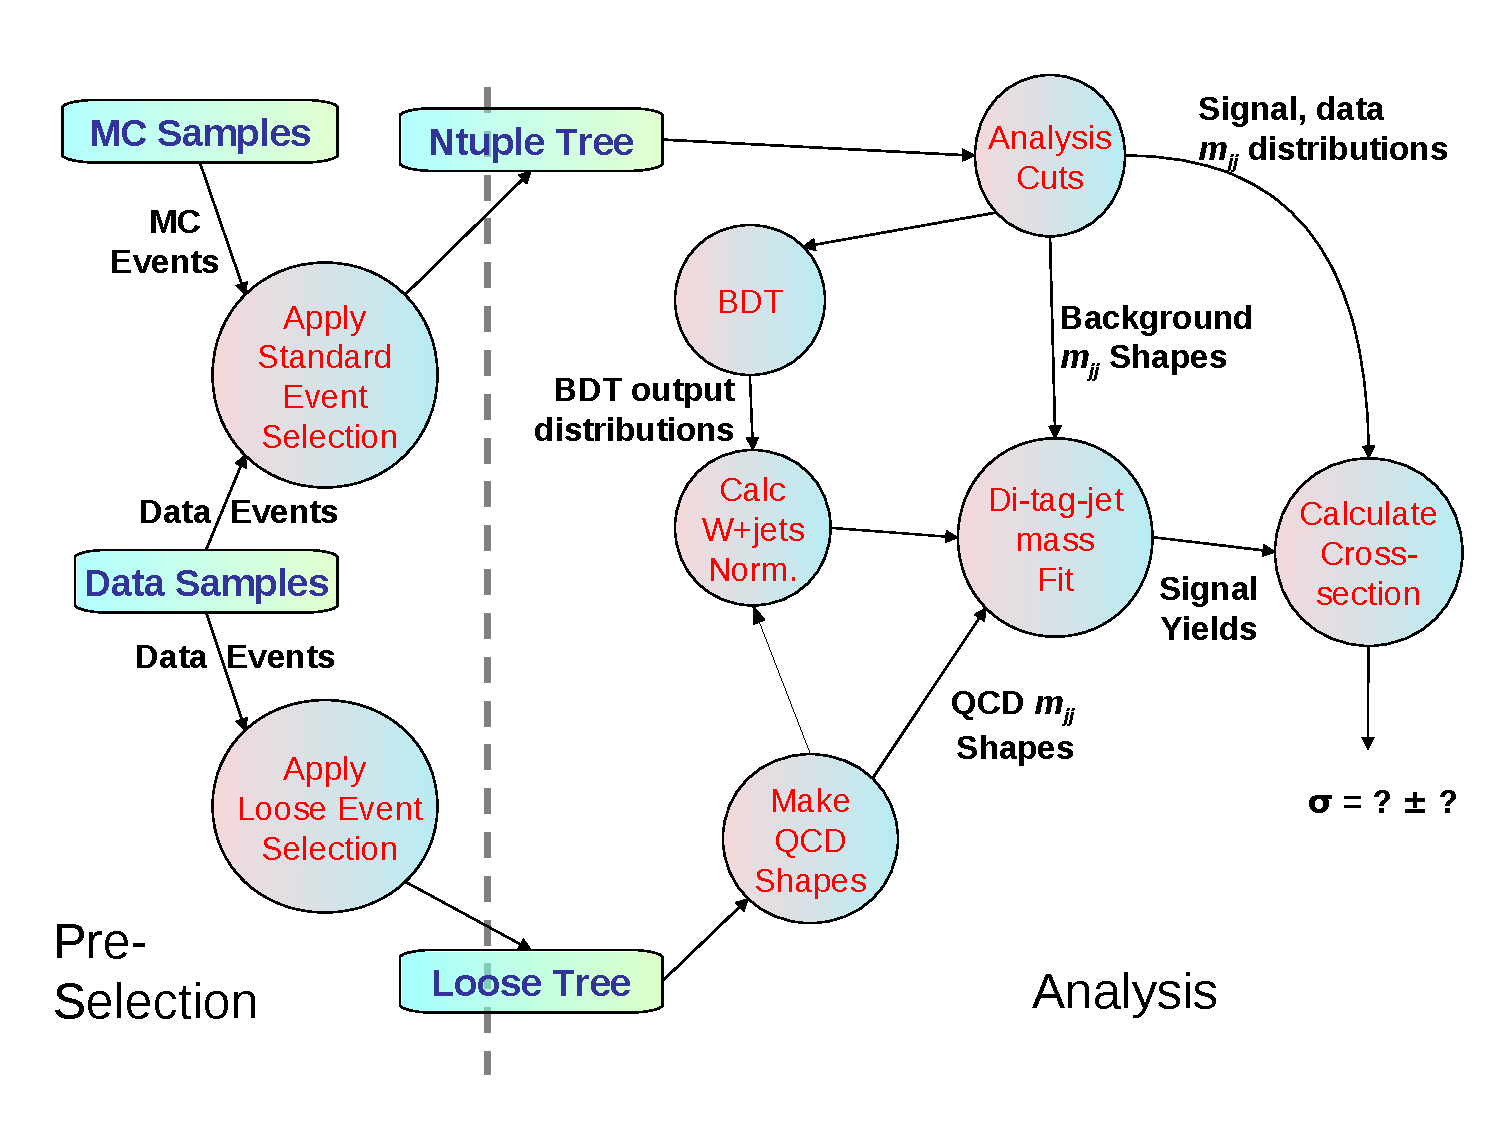
\includegraphics[width=\textwidth]{figs/mjjdfd0.pdf}
\caption{\label{fig:dfdlevel0}A schematic of the major elements of
the analysis in terms of data flows and transforms.}
\end{center}
\end{figure}
%%%%%%%%%%%%%%%%%%%

%%%%%%%%%%%%%%%%%%%%%%%%%%%%%%%%%%%%%%%%%%%%%%%%%%%%%%%%%%%%%%%%%%%%%%%%%%
%%%%%%%%%%%%%%%%%%%%%%%%%%%%%%%%%%%%%%%%%%%%%%%%%%%%%%%%%%%%%%%%%%%%%%%%%%
\clearpage{}
\section{Physics objects reconstruction}
\label{sec:reco}
\label{sec:firstStep}
% ---- ---- ---- ---- ---- ---- ---- ---- ---- ---- ---- ---- ---- ---- ----
The study of the $WV\gamma$ final state involves reconstruction of variety of physics object - electrons, muons missing transverse energy, jets and photons. 
In this section we describe in details the all physics objects involved in the analysis. 


The analysis relies on the standard reconstruction algorithms
produced by the CMS community. Event data is reconstructed using the 
particle-flow (PF) reconstruction technique~\cite{pflow}. Particle flow 
attempts to reconstruct all stable particles in an event by combining 
information from all sub-detectors. The algorithm categorizes all particles 
into the following five types: muons, electrons, photons, charged and 
neutral hadrons. The list of reconstructed particles is used as the set of
inputs for a jet clustering algorithm to create particle-flow jets.
%%%%%%%%%%%%%%%%%%%%%%%%%%%%
\subsection{Electron selection}
\label{sec:electron_cuts}

Electrons are reconstructed using a gaussian-sum filter (GSF)
algorithm \cite{CMS-PAS-EGM-10-004}, and are required to pass electron
ID cuts according to a multi-variate identification
technique~\cite{cite:elemva}.  We also require that selected
electron candidates are isolated. Particle flow-based relative
isolation is defined as
%%%
\begin{equation*}
\mathrm{RelIso_{\mathrm{PF}}} = \frac{I_{\mathrm{CH}}+max(0,I_{\mathrm{NH}}+I_{\mathrm{PHOTON}}-(\mathrm{EA}\cdot\rho))}{E_\mathrm{T}},
\end{equation*}
%%%
where $I_{\mathrm{CH}}$, $I_{\mathrm{NH}}$ and $I_{\mathrm{PHOTON}}$
are the charged hadron, neutral hadron and photon isolation variables
(using an isolation cone of 0.3). The $I_{\mathrm{CH}}$ variable is calculated from charged hadrons, associated to the primary vertex.
The neutral hadron and photon isolation variables are corrected for
contributions from pile-up using the effective area correction \cite{EAcorrElectrons},
$(\mathrm{EA}\cdot\rho)$, where $\mathrm{EA}$ is the cone effective area
and $\rho$ is the average neutral particle density of the event.

The ID and isolation cuts used are shown in Table~\ref{tab:EleID} and
have been tuned by Egamma POG to give the same efficiency bin-by-bin with respect to
the working point (WP) used for 2011 analysis.

Additionally, we require
%%%%%%%%%%%%%%%%%%%
\begin{itemize}
\item Electron $E_\mathrm{T} > 30\,\mathrm{GeV}$.
\item Pseudorapidity $|\eta| < 2.5$. There is an exclusion range due
        to the ECAL barrel-endcap transition region, defined by
        $1.4442 < |\eta_{\mathrm{sc}}| < 1.566$, where
        $\eta_{\mathrm{sc}}$ is the pseudorapidity of the ECAL
        supercluster.
%\item Impact parameter: We cut on the absolute value of the impact
%       parameter calculated with respect to the average primary vertex (PV). We
%       require: $d_0(\mathrm{PV}) < 0.02\,\mathrm{cm}.$

%\item In order to make sure that the selected electron and the selected
%jets come from the same hard interaction and not from pile up events,
%we require that the $z$ coordinate of the PV of the event and the $z$
%coordinate of the electron's vertex lie within a distance of
%less than $0.1~\mathrm{cm}$.


\item
In order to reject events in which the electron candidate actually
originates from a conversion of a photon into an $e^{+}e^{-}$ pair, we
use an approach using the vertex fit probability of fully
reconstructed conversions combined with the requirement that the
number of missed inner tracker layers of the electron track must be
exactly zero (i.e. there are no missed layers before the first hit of
the electron track from the beam line).
\end{itemize}

\begin{table}[bthp]
\begin{center}
{\footnotesize
\begin{tabular}{|c|c|c|c|}
\hline
Lepton $\eta$ & $|\eta| < 0.8$ & $0.8 < |\eta| < 1.479$ & $1.479 < |\eta| < 2.5$  \\
\hline
ID MVA cut value (tight lepton) & 0.913 & 0.964 & 0.899 \\
Isolation cut value (tight lepton) & 0.105 & 0.178 & 0.150 \\
ID MVA cut value (loose lepton) & 0.877 & 0.811 & 0.707 \\
Isolation cut value (loose lepton) & 0.426 & 0.481 & 0.390 \\
\hline
\end{tabular}
\caption[.]{\label{tab:EleID} Cut values for electron identification
MVA output and for isolation which are tuned to give the same
efficiency as VBTF Working Point (WP) 80, as used for the tight
electron selection, and VBTF Working Point (WP) 90, as used in the
loose electron selection.}}
\end{center}
\end{table}


%%%%%%%%%%%%%%%%%%%
%%%%%%%%%%%%%%%%%%%%%%%%%%%%%%%%%%%%%%%%%%%%%%%%%%%%%%%%%%%%%%%%%%%%%%%%%%%%
%%%%%%%%%%%%%%%%%%%%%%%%%%%%%%%%%%%%%%%%%%%%%%%%%%%%%%%%%%%%%%%%%%%%%%%%%%%%
\subsection{Muon selection}
\label{sec:muon_cuts}

Muon candidates are identified by two different
algorithms~\cite{MUONPAS}: one proceeds from the inner tracker outwards,
the other one starts from tracks measured in the muon chambers and matches
and combines them with tracks reconstructed in the inner tracker.
These selection criteria\cite{muonIDtwiki} are summarized below:
%%%%%%%%%%%%%%%%%%%
\begin{itemize}
\item The muon candidate is reconstructed both as a global muon and
as a tracker muon.
\item Number of pixel hits of the Tracker track $\ge 1$;
\item Number of muon system hits of the Global track $\ge 1$;
\item Normalized $\chi^{2}$ of the Global track $< 10.0$.
\item Muon $p_{\mathrm{T}} > 25\,\mathrm{GeV}$.
\item Pseudorapidity $|\eta| < 2.1$.
\item Impact parameter: We cut on the absolute value of the impact
parameter calculated with respect to the primary vertex. We require:
$d_0(\mathrm{PV}) < 0.02\,\mathrm{cm}.$
\item In order to make sure that the selected muon and the selected
jets come from the same hard interaction and not from pile up events,
we require that the $z$ coordinate of the PV of the event and the $z$
coordinate of the muon's inner track vertex lie within a distance of
less than 0.5~cm.
\item The number of tracker layers with hits from the muon track has to be
$N_{\mathrm{layers}} > 5$.
\end{itemize}

The selected muon candidates also have to be isolated. Particle
flow-based relative isolation for muons is defined as
\begin{equation*}
\mathrm{RelIso_{\mathrm{PF}}} = \frac{I_{\mathrm{CH}}+max(0,I_{\mathrm{NH}}+I_{\mathrm{PHOTON}}-(0.5~{p}_{T}^\mathrm{sumPU}))}{p_\mathrm{T}},
\end{equation*}

where $I_{\mathrm{CH}}$, $I_{\mathrm{NH}}$ and $I_{\mathrm{PHOTON}}$
are the charged hadron, neutral hadron and photon isolation variables
(using an isolation cone of 0.4). The charged hadron isolation variable uses tracks from the primary vertices only. 
The neutral hadron and photon isolation variables are corrected for
contributions from pile-up using the DeltaBeta correction, $(0.5
p_T^\mathrm{sumPU})$. We require the muon to have
$\mathrm{RelIso_{\mathrm{PF}}} < 0.12$ in order to be considered
isolated.


\subsubsection{Loose Electron}
For the purposes of rejecting events with more than one lepton we
define a loose electron, which has looser cuts. We consider electrons
which have $p_{\mathrm{T}} > 20\,\mathrm{GeV}/c$, $|\eta| < 2.5$,
and which satisfy electron $\mathrm{RelIso_{\mathrm{PF}}}$ and MVA ID
cuts. The cut values for the electron ID and isolation used in the
analysis can be found in Table~\ref{tab:EleID}.
%As in the case of the
%tight electrons, we also require $d_0(\mathrm{PV}) <
%0.02\,\mathrm{cm}$ and that the $z$ coordinate of the PV of the event
%and the $z$ coordinate of the electron's vertex lie within a distance
%of less than $0.1~\mathrm{cm}$.

\subsubsection{Loose Muon}
Additionally, to reject events with more than one lepton, we define a
loose muon, which has looser cuts. We consider all global muons which
have $p_{\mathrm{T}} > 10\,\mathrm{GeV}/c$, $|\eta| < 2.5$, and
$\mathrm{RelIso_{\mathrm{PF}}} < 0.2$ to be loose muons.

%%%%%%%%%%%%%%%%%%%%%%%%%%%%%%%%%%%%%%%%%%%%%%%%%%%%%%%%%%%%%%%%%%%%%%%%%%%%
%%%%%%%%%%%%%%%%%%%%%%%%%%%%%%%%%%%%%%%%%%%%%%%%%%%%%%%%%%%%%%%%%%%%%%%%%%%%
%%%%%%%%%%%%%%%%%%%%%%%%%%%%%%%%%%%%%%%%%%%%%%%%%%%%%%%%%%%%%%%%%%%%%%%%%%%%
%%%%%%%%%%%%%%%%%%%%%%%%%%%%%%%%%%%%%%%%%%%%%%%%%%%%%%%%%%%%%%%%%%%%%%%%%%%%
\subsection{Jet selection}
\label{sec:firstStep_jets}
Jets are reconstructed with the anti-KT algorithm \cite{cacciari},
starting from the set of objects reconstructed by the particle
flow \cite{pflow,CMS-PAS-JME-10-003,CMS-PAS-PFT-10-002}.
Jets are corrected such that the measured energy of the jet
correctly reproduces the energy of the initial particle.
The CMS standard L2 (relative) correction makes the jet response flat in $\eta$.
The standard L3 (absolute) correction brings the jet closer to the $\PT$ of
a matched generated jet created using generator level input and a similar
jet clustering algorithm.
The L2 and L3 corrections are calculated using Monte Carlo, and thus a
L2L3 residual correction is applied that fixes the discrepancies between
Monte Carlo and data~\cite{newjes-cms}.
In this analysis we use jets with measured (corrected) $\PT$
greater than 30~$\gev$.
We require $|\eta| < 2.4$ so that the jets fall within the
tracker acceptance.  Jets from pile-up are identified and removed with PileupJetID tool ~\cite{cite:PileupJetID}.

Jets are required to pass a set of loose identification
criteria; this requirement eliminates jets originating from or being seeded by
noisy channels in the calorimeter~\cite{Chatrchyan:2009hy}:

%%%%%%%%%%%%%%
\begin{itemize}
\item Fraction of energy due to neutral hadrons $<$ 0.99.
\item Fraction of energy due to neutral EM deposits $<$ 0.99.
\item Number of constituents $>$ 1.
\item Number of charged hadrons candidates $>$ 0.
\item Fraction of energy due to charged hadrons candidates $>$ 0.
\item Fraction of energy due to charged EM deposits $<$ 0.99.
\end{itemize}
%%%%%%%%%%
All energy fractions are calculated from uncorrected jets.

\par
In order to account for electron and muon objects that
have been reconstructed as jets, we remove from the jet
collection any jet that falls within a
cone of radius $R= 0.3$ of a loose electron or a loose muon.
This ``cleaning'' procedure is applied in order to ensure that the same
particle is not double counted as two different physics objects.

%%%%%%%%%%%%%%%%%%%%%%%%%%%%%%%%%%%%%%%%%%%%%%%%%%%%%%
%%%%%%%%%%%%%%%%%%%%%%%%%%%%%%%%%%%%%%%%%%%%%%%%%%%%%%
\subsection{Missing Transverse Energy (\MET)}
\label{sec:MET}
An accurate \MET measurement is essential for distinguishing
the $\Wo$ signal from QCD backgrounds.
We use the \MET estimate provided by the Particle Flow algorithm.
PF \MET showed the best performance
among several \MET algorithms~\cite{PFMET}.
The \MET is computed as the vector sum of all PF objects.
It has energy scale correction (type 1) and also "shift" correction, which account for small misalignment of various sub-detector systems.
A good agreement is found between the \MET
distributions of $\Wln$ events in data and simulation~\cite{metPAS}.
The resolution for inclusive multi-jet samples and for
$\Wln$ events is also well reproduced by the simulation.
A relative broadening of a few percent is observed in the data compared to MC,
and has a negligible impact on the
extraction of the W yields~\cite{WZCMS:2010}.
We reject events with small opening angle between \MET and any of the two leading jest ($\Delat\phi(\MET,j)<0.4$). 
This cut rejects events with fake \MET due to a mismeasured jet $p_T$.  

%%%%%%%%%%%%%%%%%%%%%%%
\section{Event selection}
\label{sec:evtSel}


The event should have a good primary vertex (PV). This means selecting
the primary vertex with the highest sum of $p_{T}^2$ of the tracks
associated with it and requiring it to have a number of degrees of
freedom (ndof) $\ge 4$, where ndof corresponds to the weighted sum of
the number of tracks used for the construction of the PV. In addition,
the PV must lie in the central detector region of $|z| \le 24$~cm
and $\rho \le 2$~cm around the nominal interaction point.

\par
In the electron channel, we select events that contain exactly one
tight electron candidate fulfilling the criteria described in
Section~\ref{sec:electron_cuts} and reject events that contain a
loose electron or a loose muon in addition to the tight electron.
In the muon channel, we select events that contain exactly one
tight muon candidate whose criteria are described in
Section~\ref{sec:muon_cuts} and reject events that contain an
additional loose lepton.
In both channels we require an event to have missing transverse energy
\MET in excess of 35~GeV and to have transverse mass greater than
30~GeV.  These cuts are designed to reduce the background
from QCD multijet production.

Further we require two central jets in the event with di-jet invariant mass 70<$m_{jj}$<100 GeV which corresponds to the hadronic decay of the W or Z in the signal process 
and $\Delat\eta(j,j)<1.4$ which further suppresses the $W\gamma+jets$ background. Additionally we require both jets to fail the CSV-medium b-tag requirement, which suppresses 
the $t\overline{t}\gamma$ and single top backgrounds. In the electron channel we require $|M_{e\gamma}-M_{Z}|>10$ GeV, which efficiently rejects the 
$Z+jets$ background, when one of the leptons in $e^+e^-$ pair is misreconstructed as photon. 


%We further require exactly two jets passing the cuts
%described in Section~\ref{sec:firstStep_jets}.


\section{Lepton reconstruction, selection and trigger efficiencies}\label{sec:Eff}

Since the lepton reconstruction, selection, and trigger efficiencies can be slightly different between data and simulation,
correction factors have to be applied to the MC to account for these differences. The efficiencies are calculated using a Tag and Probe
technique exploiting Z boson decays to a pair of electrons or muons, respectively. One of the leptons is used as tag and has to pass a
tight selection, while the second one is used as probe if the tag-probe pair combines to the Z boson mass. The total lepton efficiency
can be factorized into three components:

\begin{equation}
\epsilon_{\textnormal{total}}=\epsilon_{\textnormal{Reco}}\cdot\epsilon_{\textnormal{Id}}\cdot\epsilon_{\textnormal{HLT}}
\end{equation}

The tag and probe method is nearly the same compared to the one already used in the 2011 data analysis for this Higgs search
(\cite{CMS-AN-12-029},\cite{CMS-AN-2012-021}). Therefore, only the most important information will be discussed.

\subsection{Electron efficiencies}\label{subsec:EffEle}
In the electron case, the reconstruction efficiency $\epsilon_{\textnormal{Reco}}$ characterizes the transition from a supercluster in the
electromagnetic calorimeter to a reconstructed Particle Flow electron. The ability of a reconstructed electron to pass the offline
selection, consisting of several isolation and identification criteria, is given by the identification efficiency $\epsilon_{\textnormal{Id}}$.
Finally, the selected electron has a certain probability to fire the high level trigger and the efficiency to fulfill the HLT requirements
is parametrized as $\epsilon_{\textnormal{HLT}}$. In data, a single electron trigger is used at HLT level, while in MC the HLT requirements are dropped. \\
Since the HLT efficiency is MC is equal to $100\%$, the HLT efficiency measured on data is applied directly in the analysis of MC samples,
while the other two efficiency components are calculated both for data and MC, so that a data/MC scale factor is applied in the other cases. \\
In general, since the efficiency depends both on $\pt$ and $\eta$ of the electron, the measurement is binned in $\pt$ as (30, 35, 40, 45, 50, 200)\GeVc
and in $\eta$ as (-2.5, -1.5, 0.0, 1.5, 2.5) of the probe electron. The resulting efficiencies and scale factors are summarized in Table~\ref{tab:eleEff} and
shown in Figure~\ref{fig:eleEff}.

\begin{table}[htb]
\centering
\scalebox{0.70}{
  \begin{tabular}{|c|c|c|c|c|c|c|}
  \hline
  $p_{\textnormal{T,min}}$ & $p_{\textnormal{T,max}}$ & $\eta_{\textnormal{min}}$ & $\eta_{\textnormal{max}}$ & $\epsilon_{\textnormal{Reco,data}}$/$\epsilon_{\textnormal{Reco,mc}}$ & $\epsilon_{\textnormal{ID,data}}$/$\epsilon_{\textnormal{ID,mc}}$ & $\epsilon_{\textnormal{HLT,data}}$ \\
  $[\GeVc]$         & $[\GeVc]$         &                     &                     &                              &                           &                               \\
  \hline
  \hline
  30 & 35 & -2.5 & -1.5 & 1.000 $\pm$ 0.002 & 0.973 $\pm$ 0.004 & 0.639 $\pm$ 0.003 \\
  30 & 35 & -1.5 & 0 & 0.996 $\pm$ 0.001 & 0.981 $\pm$ 0.003 & 0.874 $\pm$ 0.001 \\
  30 & 35 & 0 & 1.5 & 0.996 $\pm$ 0.001 & 0.980 $\pm$ 0.003 & 0.874 $\pm$ 0.001 \\
  30 & 35 & 1.5 & 2.5 & 1.002 $\pm$ 0.001 & 0.999 $\pm$ 0.004 & 0.650 $\pm$ 0.003 \\
  35 & 40 & -2.5 & -1.5 & 1.001 $\pm$ 0.001 & 1.005 $\pm$ 0.003 & 0.686 $\pm$ 0.002 \\
  35 & 40 & -1.5 & 0 & 0.999 $\pm$ 0.001 & 0.978 $\pm$ 0.002 & 0.896 $\pm$ 0.001 \\
  35 & 40 & 0 & 1.5 & 0.998 $\pm$ 0.001 & 0.978 $\pm$ 0.002 & 0.891 $\pm$ 0.002 \\
  35 & 40 & 1.5 & 2.5 & 1.001 $\pm$ 0.001 & 1.003 $\pm$ 0.085 & 0.690 $\pm$ 0.002 \\
  40 & 45 & -2.5 & -1.5 & 1.001 $\pm$ 0.001 & 1.005 $\pm$ 0.003 & 0.708 $\pm$ 0.002 \\
  40 & 45 & -1.5 & 0 & 0.999 $\pm$ 0.001 & 0.985 $\pm$ 0.001 & 0.909 $\pm$ 0.001 \\
  40 & 45 & 0 & 1.5 & 0.999 $\pm$ 0.001 & 0.983 $\pm$ 0.001 & 0.906 $\pm$ 0.001 \\
  40 & 45 & 1.5 & 2.5 & 1.000 $\pm$ 0.001 & 1.014 $\pm$ 0.003 & 0.720 $\pm$ 0.002 \\
  45 & 50 & -2.5 & -1.5 & 1.001 $\pm$ 0.001 & 1.017 $\pm$ 0.003 & 0.724 $\pm$ 0.002 \\
  45 & 50 & -1.5 & 0 & 1.000 $\pm$ 0.001 & 0.984 $\pm$ 0.002 & 0.917 $\pm$ 0.001 \\
  45 & 50 & 0 & 1.5 & 0.999 $\pm$ 0.001 & 0.985 $\pm$ 0.002 & 0.911 $\pm$ 0.001 \\
  45 & 50 & 1.5 & 2.5 & 1.001 $\pm$ 0.001 & 1.021 $\pm$ 0.003 & 0.733 $\pm$ 0.002 \\
  50 & 200 & -2.5 & -1.5 & 0.999 $\pm$ 0.001 & 1.023 $\pm$ 0.003 & 0.733 $\pm$ 0.003 \\
  50 & 200 & -1.5 & 0 & 0.999 $\pm$ 0.001 & 0.990 $\pm$ 0.002 & 0.925 $\pm$ 0.001 \\
  50 & 200 & 0 & 1.5 & 0.999 $\pm$ 0.001 & 0.991 $\pm$ 0.003 & 0.920 $\pm$ 0.001 \\
  50 & 200 & 1.5 & 2.5 & 1.000 $\pm$ 0.001 & 1.019 $\pm$ 0.003 & 0.745 $\pm$ 0.003 \\
  \hline
  \end{tabular}}
\caption{Electron efficiency and data/MC scale factors for super-cluster to reconstructed electrons ($\epsilon_{\textnormal{Reco}}$),
    reconstructed to selected electrons ($\epsilon_{\textnormal{ID}}$) and selected to HLT electrons ($\epsilon_{\textnormal{HLT}}$).
    The errors are statistical only.}
\label{tab:eleEff}
\end{table}

\begin{figure}[b]
  \begin{center}
    \subfigure[]{
    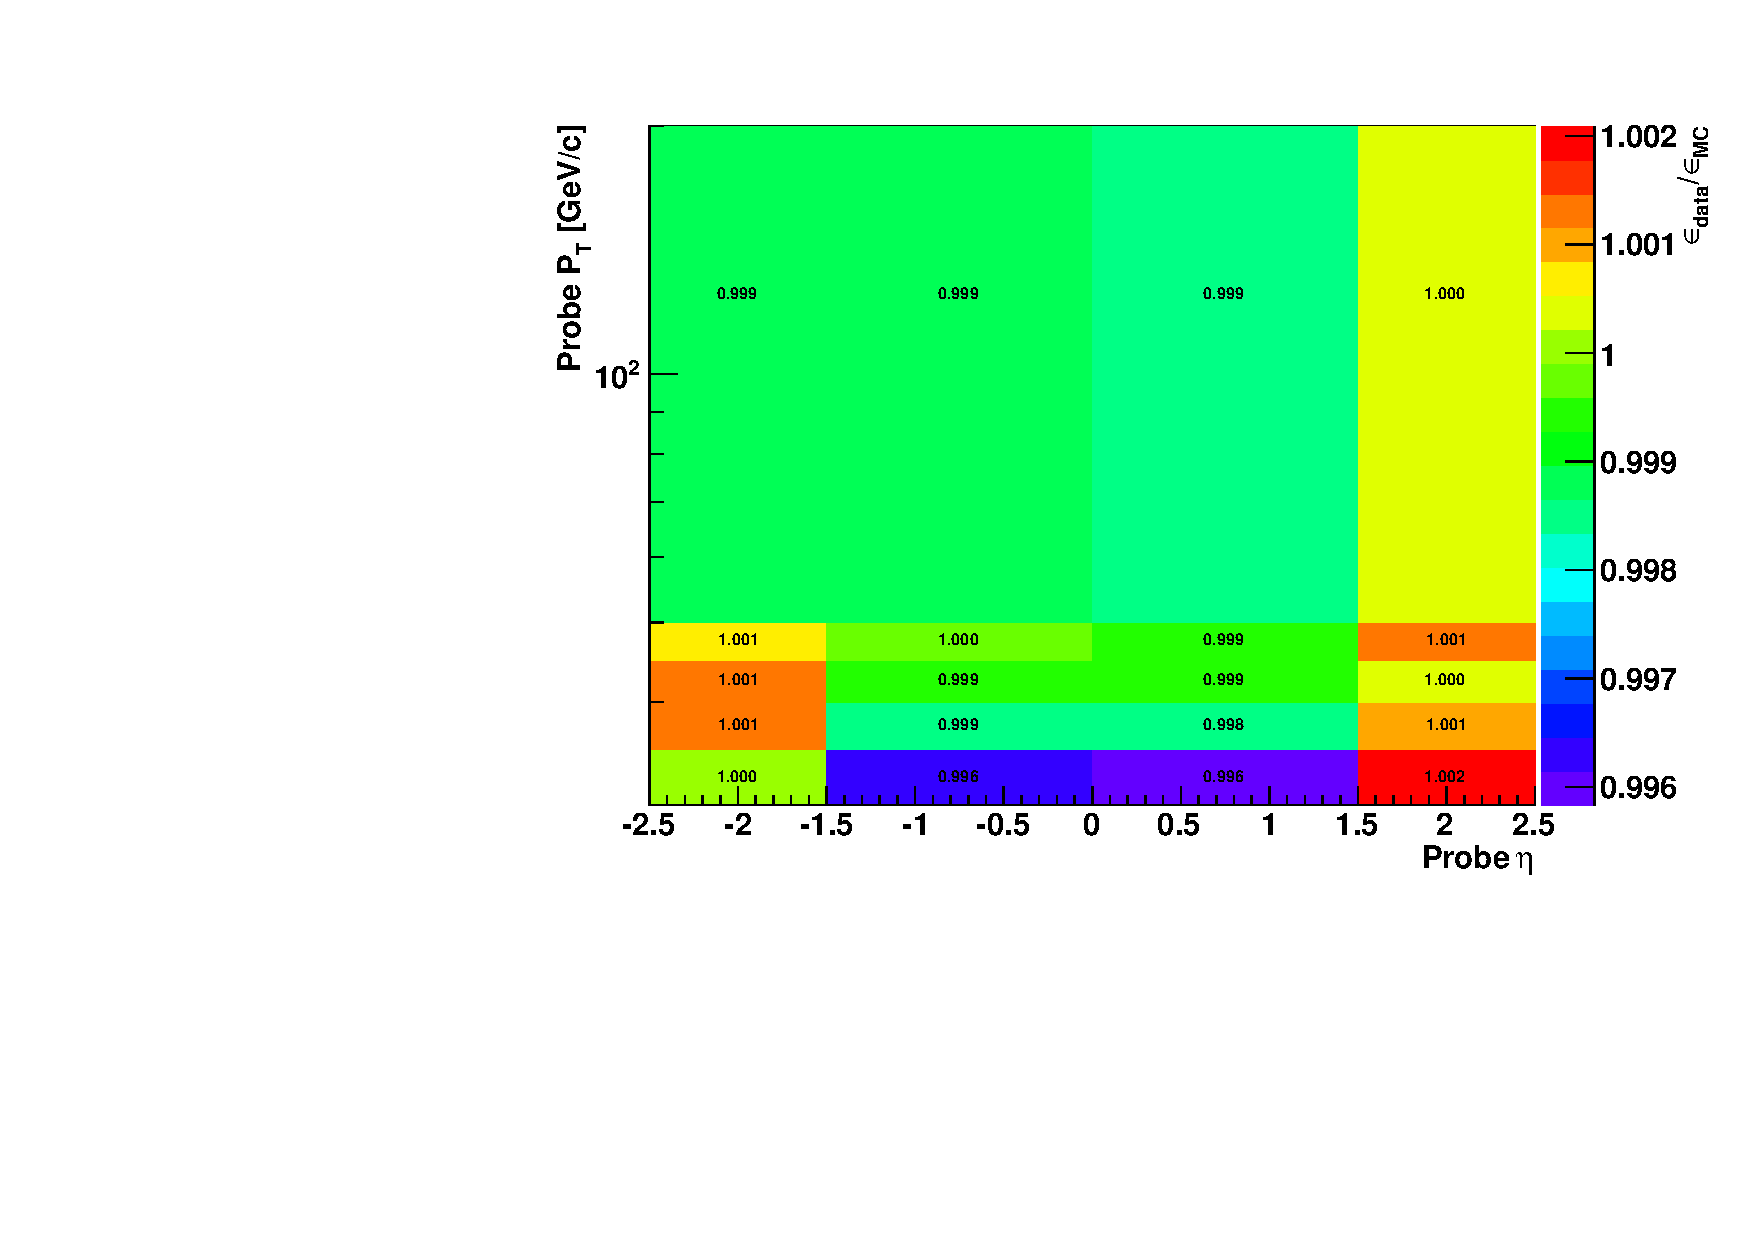
\includegraphics[width=0.32\textwidth]{figs/scaleFactor-Run2012ABC-SCToElectron.pdf}
  }
    \subfigure[]{
    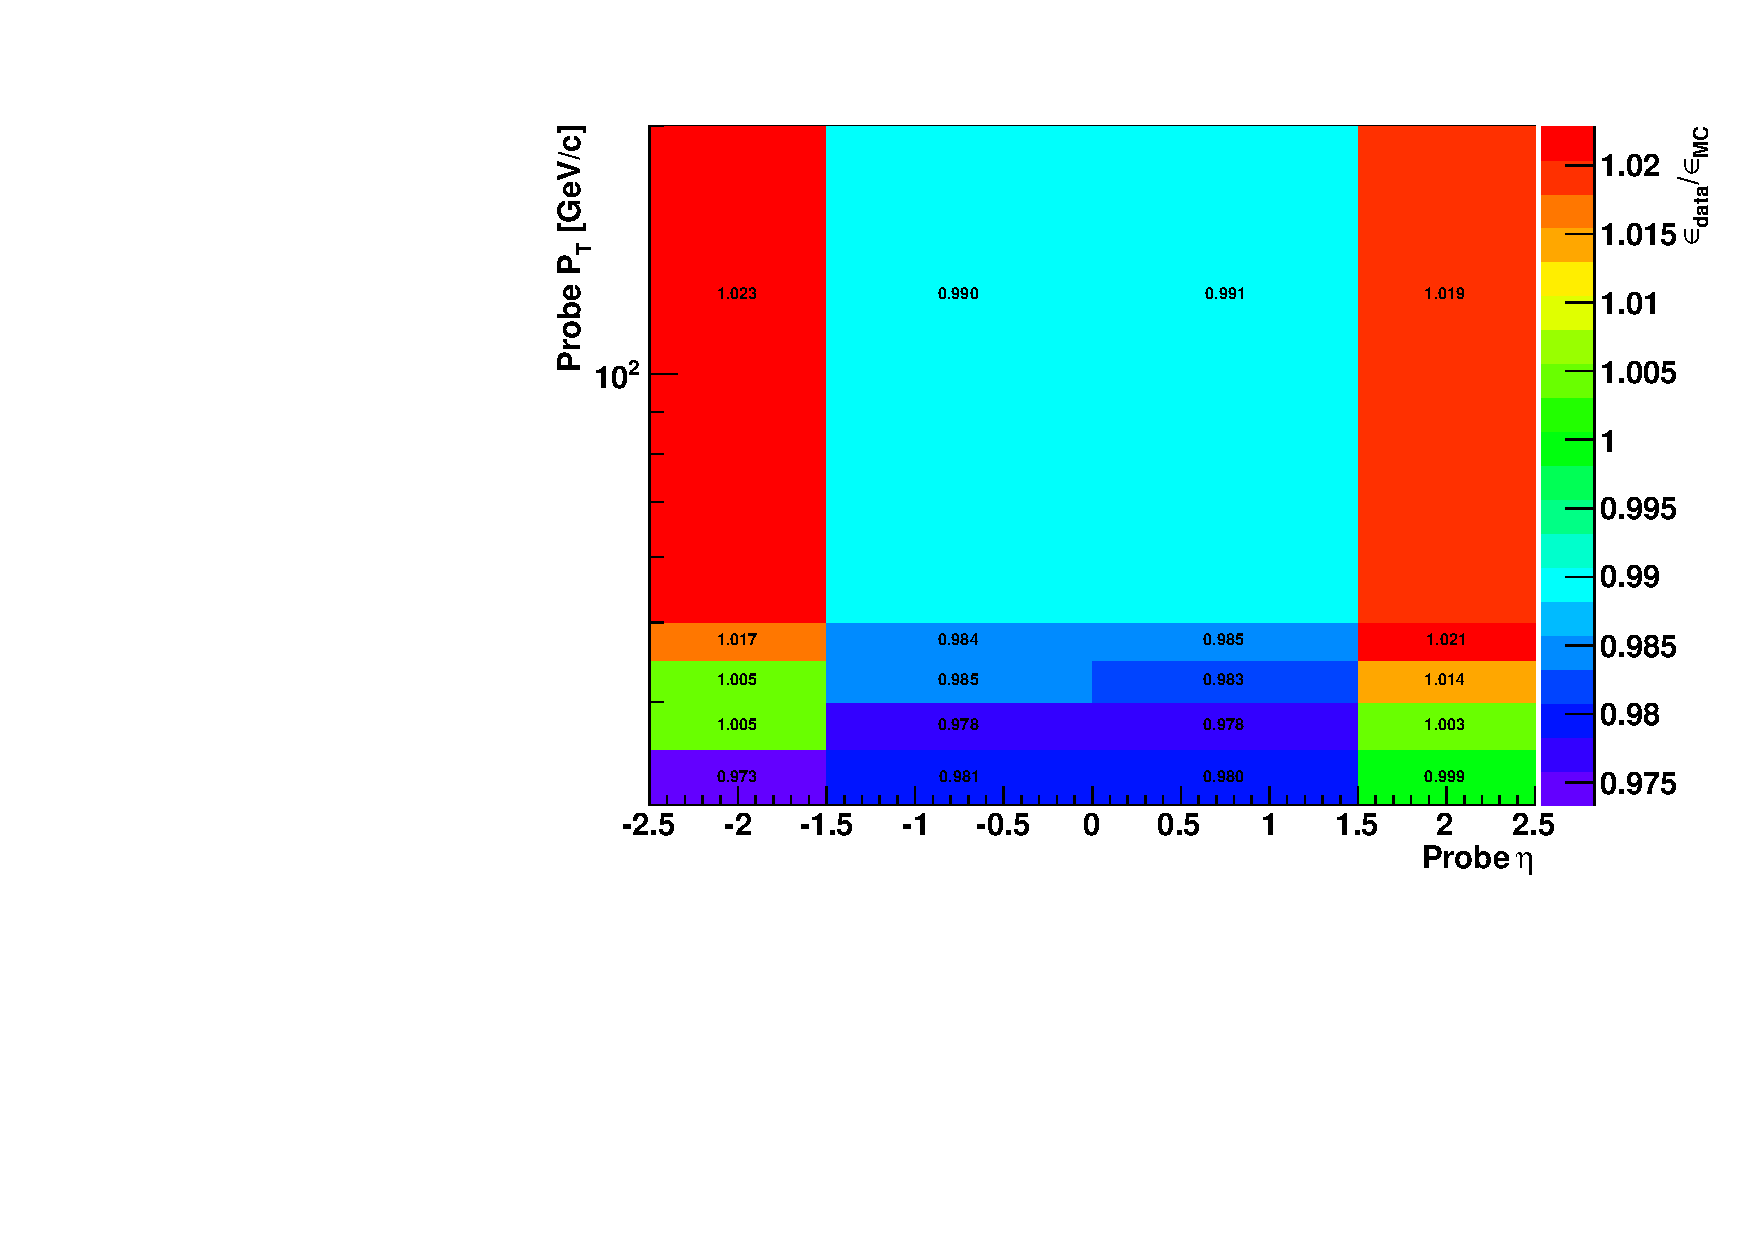
\includegraphics[width=0.32\textwidth]{figs/scaleFactor-Run2012ABC-GsfElectronToId.pdf}
  }
  \subfigure[]{
    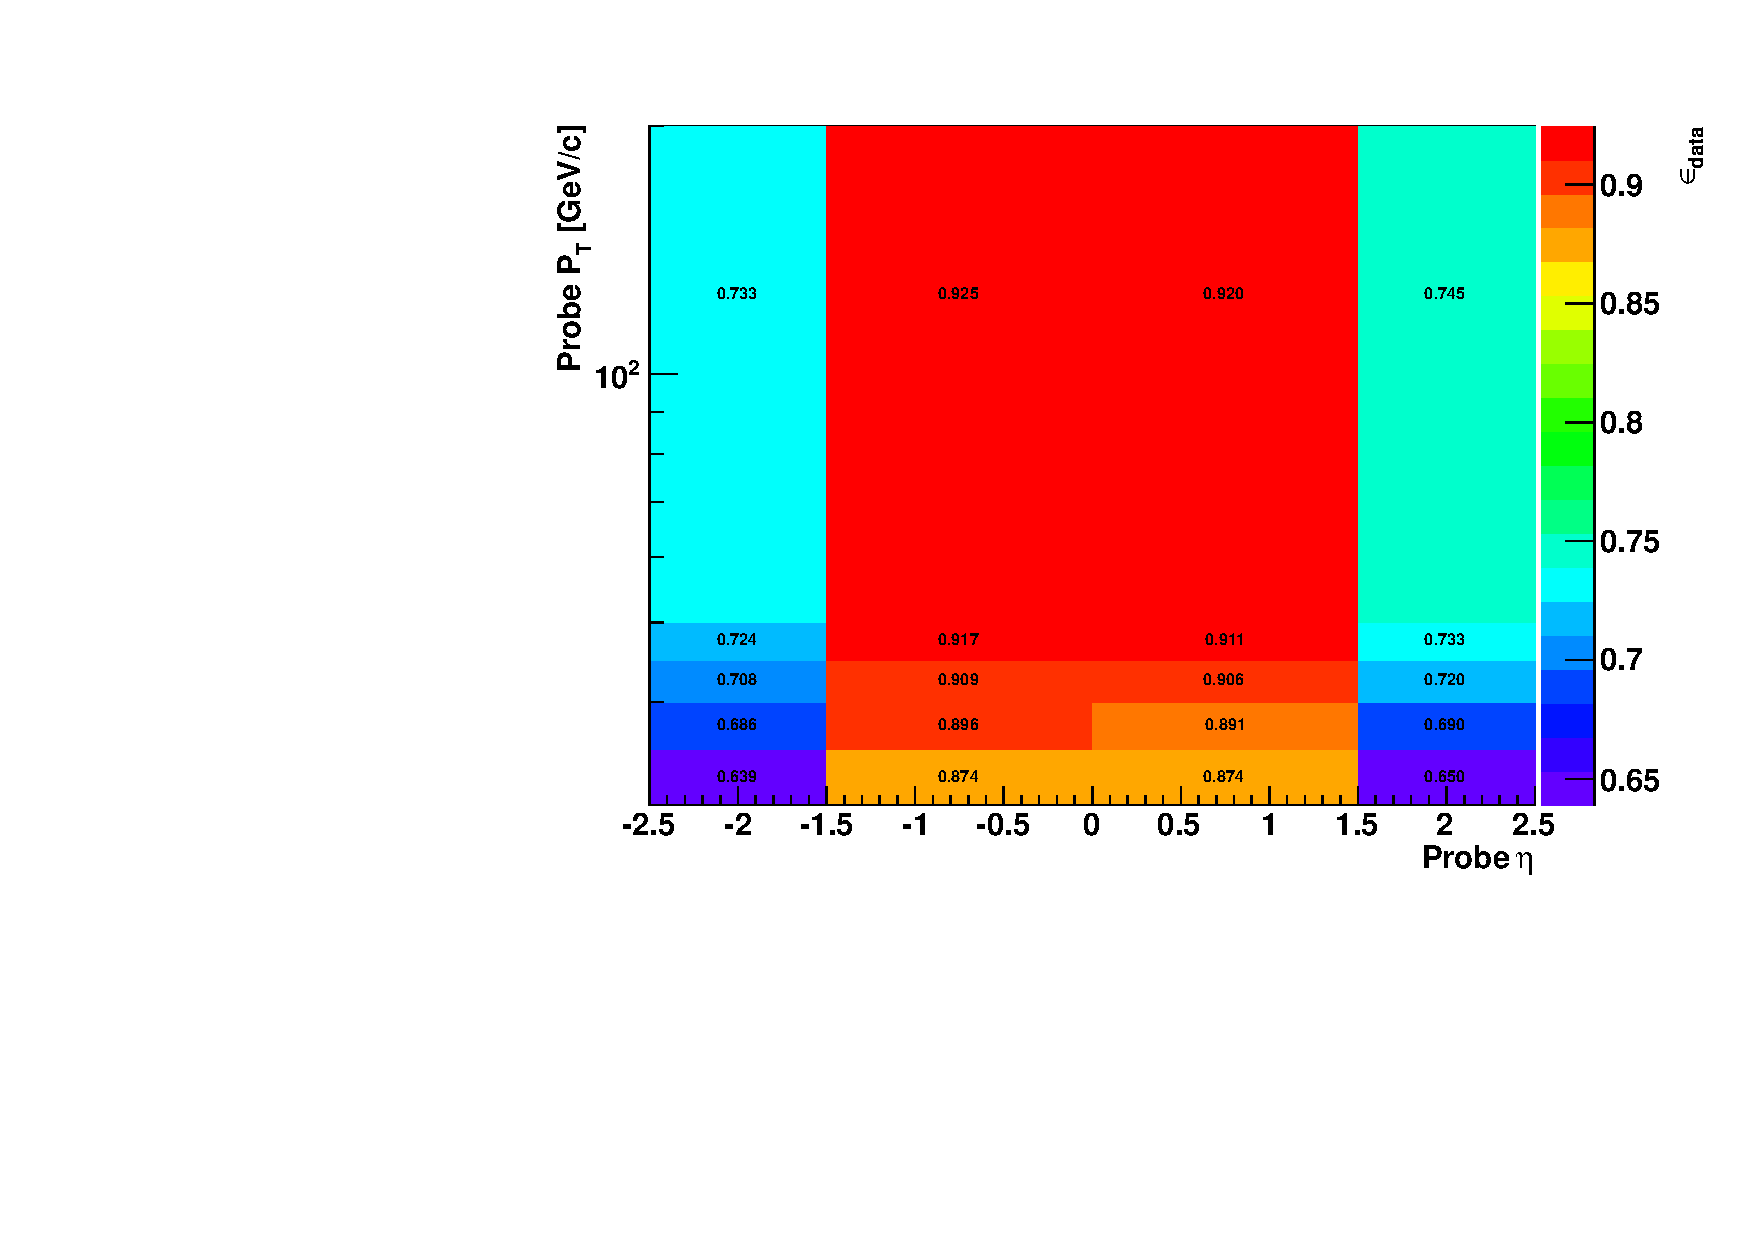
\includegraphics[width=0.32\textwidth]{figs/efficiency-Run2012ABC-WP80ToHLTEle.pdf}
  }
    \caption{Electron efficiency and data/MC scale factors for super-cluster to reconstructed electrons $\epsilon_{\textnormal{Reco}}$ (a),
    reconstructed to selected electrons $\epsilon_{\textnormal{Id}}$ (b) and selected to HLT electrons
      $\epsilon_{\textnormal{HLT}}$ (c).}
    \label{fig:eleEff}
  \end{center}
\end{figure}

\subsection{Muon efficiencies}\label{subsec:EffMu}

In the muon case, the reconstruction efficiency $\epsilon_{\textnormal{Reco}}$ describes the ability to reconstruct a Particle Flow muon starting with
a particle track and can be assumed to be one \cite{MUONPAS}. The identification efficiency $\epsilon_{\textnormal{Id}}$ gives an estimate for a
reconstructed muon to pass the offline selection criteria. It can be computed for both data and simulation and thus a scale factor,
the ratio of the two efficiencies, is derived. \\
The trigger efficiency $\epsilon_{\textnormal{HLT}}$  is the fraction of selected muons fulfilling the HLT requirements, and, since the HLT
requirement is dropped on the MC analysis, the efficiency computed on data is used directly to correct the MC event expectation.\\
The efficiency measurement is binned both in $\pt$ and $\eta$ of the probe muon covering the
relevant intervals (25, 30, 35, 40, 45, 50, 200)\GeVc in $\pt$ and (-2.1, -1.5, -1.0, -0.5, 0.0, 0.5, 1.0, 1.5, 2.1) in $\eta$. The resulting selection
and trigger efficiencies and scale factors are summarized in Table~\ref{tab:muonEff} and Figure~\ref{fig:muonEff}.

\begin{table}[htb]
\centering
\scalebox{0.70}{
  \begin{tabular}{|c|c|c|c|c|c|}
  \hline
  $p_{\textnormal{T,min}}$ & $p_{\textnormal{T,max}}$ & $\eta_{\textnormal{min}}$ & $\eta_{\textnormal{max}}$ & $\epsilon_{\textnormal{ID,data}}$/$\epsilon_{\textnormal{ID,mc}}$ & $\epsilon_{\textnormal{HLT,data}}$ \\
  $[\GeVc]$         & $[\GeVc]$         &                     &                     &                             &                               \\
  \hline
  \hline
  25 & 30 & -2.1 & -1.5 & 0.992 $\pm$ 0.003 & 0.766 $\pm$ 0.003 \\
  25 & 30 & -1.5 & -1 & 0.987 $\pm$ 0.003 & 0.822 $\pm$ 0.003 \\
  25 & 30 & -1 & -0.5 & 0.990 $\pm$ 0.003 & 0.914 $\pm$ 0.002 \\
  25 & 30 & -0.5 & 0 & 0.984 $\pm$ 0.003 & 0.920 $\pm$ 0.002 \\
  25 & 30 & 0 & 0.5 & 0.985 $\pm$ 0.003 & 0.924 $\pm$ 0.002 \\
  25 & 30 & 0.5 & 1 & 0.992 $\pm$ 0.003 & 0.913 $\pm$ 0.002 \\
  25 & 30 & 1 & 1.5 & 0.991 $\pm$ 0.003 & 0.802 $\pm$ 0.003 \\
  25 & 30 & 1.5 & 2.1 & 0.995 $\pm$ 0.002 & 0.814 $\pm$ 0.003 \\
  30 & 35 & -2.1 & -1.5 & 0.991 $\pm$ 0.002 & 0.785 $\pm$ 0.002 \\
  30 & 35 & -1.5 & -1 & 0.988 $\pm$ 0.002 & 0.829 $\pm$ 0.002 \\
  30 & 35 & -1 & -0.5 & 0.988 $\pm$ 0.002 & 0.921 $\pm$ 0.002 \\
  30 & 35 & -0.5 & 0 & 0.984 $\pm$ 0.002 & 0.930 $\pm$ 0.001 \\
  30 & 35 & 0 & 0.5 & 0.985 $\pm$ 0.002 & 0.935 $\pm$ 0.001 \\
  30 & 35 & 0.5 & 1 & 0.990 $\pm$ 0.002 & 0.922 $\pm$ 0.002 \\
  30 & 35 & 1 & 1.5 & 0.987 $\pm$ 0.002 & 0.807 $\pm$ 0.002 \\
  30 & 35 & 1.5 & 2.1 & 0.995 $\pm$ 0.002 & 0.833 $\pm$ 0.002 \\
  35 & 40 & -2.1 & -1.5 & 0.992 $\pm$ 0.002 & 0.793 $\pm$ 0.002 \\
  35 & 40 & -1.5 & -1 & 0.987 $\pm$ 0.002 & 0.832 $\pm$ 0.002 \\
  35 & 40 & -1 & -0.5 & 0.991 $\pm$ 0.002 & 0.926 $\pm$ 0.001 \\
  35 & 40 & -0.5 & 0 & 0.986 $\pm$ 0.002 & 0.935 $\pm$ 0.001 \\
  35 & 40 & 0 & 0.5 & 0.986 $\pm$ 0.002 & 0.940 $\pm$ 0.001 \\
  35 & 40 & 0.5 & 1 & 0.991 $\pm$ 0.002 & 0.925 $\pm$ 0.001 \\
  35 & 40 & 1 & 1.5 & 0.989 $\pm$ 0.002 & 0.812 $\pm$ 0.002 \\
  35 & 40 & 1.5 & 2.1 & 0.994 $\pm$ 0.002 & 0.837 $\pm$ 0.002 \\
  40 & 45 & -2.1 & -1.5 & 0.994 $\pm$ 0.002 & 0.800 $\pm$ 0.002 \\
  40 & 45 & -1.5 & -1 & 0.987 $\pm$ 0.001 & 0.837 $\pm$ 0.002 \\
  40 & 45 & -1 & -0.5 & 0.992 $\pm$ 0.001 & 0.927 $\pm$ 0.001 \\
  40 & 45 & -0.5 & 0 & 0.986 $\pm$ 0.001 & 0.940 $\pm$ 0.001 \\
  40 & 45 & 0 & 0.5 & 0.987 $\pm$ 0.001 & 0.944 $\pm$ 0.001 \\
  40 & 45 & 0.5 & 1 & 0.991 $\pm$ 0.001 & 0.928 $\pm$ 0.001 \\
  40 & 45 & 1 & 1.5 & 0.991 $\pm$ 0.001 & 0.817 $\pm$ 0.002 \\
  40 & 45 & 1.5 & 2.1 & 0.996 $\pm$ 0.001 & 0.844 $\pm$ 0.002 \\
  45 & 50 & -2.1 & -1.5 & 0.993 $\pm$ 0.002 & 0.807 $\pm$ 0.002 \\
  45 & 50 & -1.5 & -1 & 0.987 $\pm$ 0.002 & 0.840 $\pm$ 0.002 \\
  45 & 50 & -1 & -0.5 & 0.990 $\pm$ 0.001 & 0.931 $\pm$ 0.001 \\
  45 & 50 & -0.5 & 0 & 0.988 $\pm$ 0.002 & 0.941 $\pm$ 0.001 \\
  45 & 50 & 0 & 0.5 & 0.987 $\pm$ 0.002 & 0.947 $\pm$ 0.001 \\
  45 & 50 & 0.5 & 1 & 0.992 $\pm$ 0.001 & 0.930 $\pm$ 0.001 \\
  45 & 50 & 1 & 1.5 & 0.991 $\pm$ 0.002 & 0.821 $\pm$ 0.002 \\
  45 & 50 & 1.5 & 2.1 & 0.995 $\pm$ 0.002 & 0.851 $\pm$ 0.002 \\
  50 & 200 & -2.1 & -1.5 & 0.991 $\pm$ 0.002 & 0.809 $\pm$ 0.002 \\
  50 & 200 & -1.5 & -1 & 0.987 $\pm$ 0.002 & 0.842 $\pm$ 0.002 \\
  50 & 200 & -1 & -0.5 & 0.992 $\pm$ 0.002 & 0.931 $\pm$ 0.001 \\
  50 & 200 & -0.5 & 0 & 0.987 $\pm$ 0.002 & 0.944 $\pm$ 0.001 \\
  50 & 200 & 0 & 0.5 & 0.989 $\pm$ 0.002 & 0.946 $\pm$ 0.001 \\
  50 & 200 & 0.5 & 1 & 0.992 $\pm$ 0.002 & 0.932 $\pm$ 0.001 \\
  50 & 200 & 1 & 1.5 & 0.993 $\pm$ 0.002 & 0.824 $\pm$ 0.002 \\
  50 & 200 & 1.5 & 2.1 & 0.996 $\pm$ 0.002 & 0.854 $\pm$ 0.002 \\
  \hline
  \end{tabular}}
\caption{Muon selection scale factors and HLT efficiencies. The errors are statistical only.}
\label{tab:muonEff}
\end{table}


\begin{figure}[t]
  \begin{center}
    \subfigure[]{
    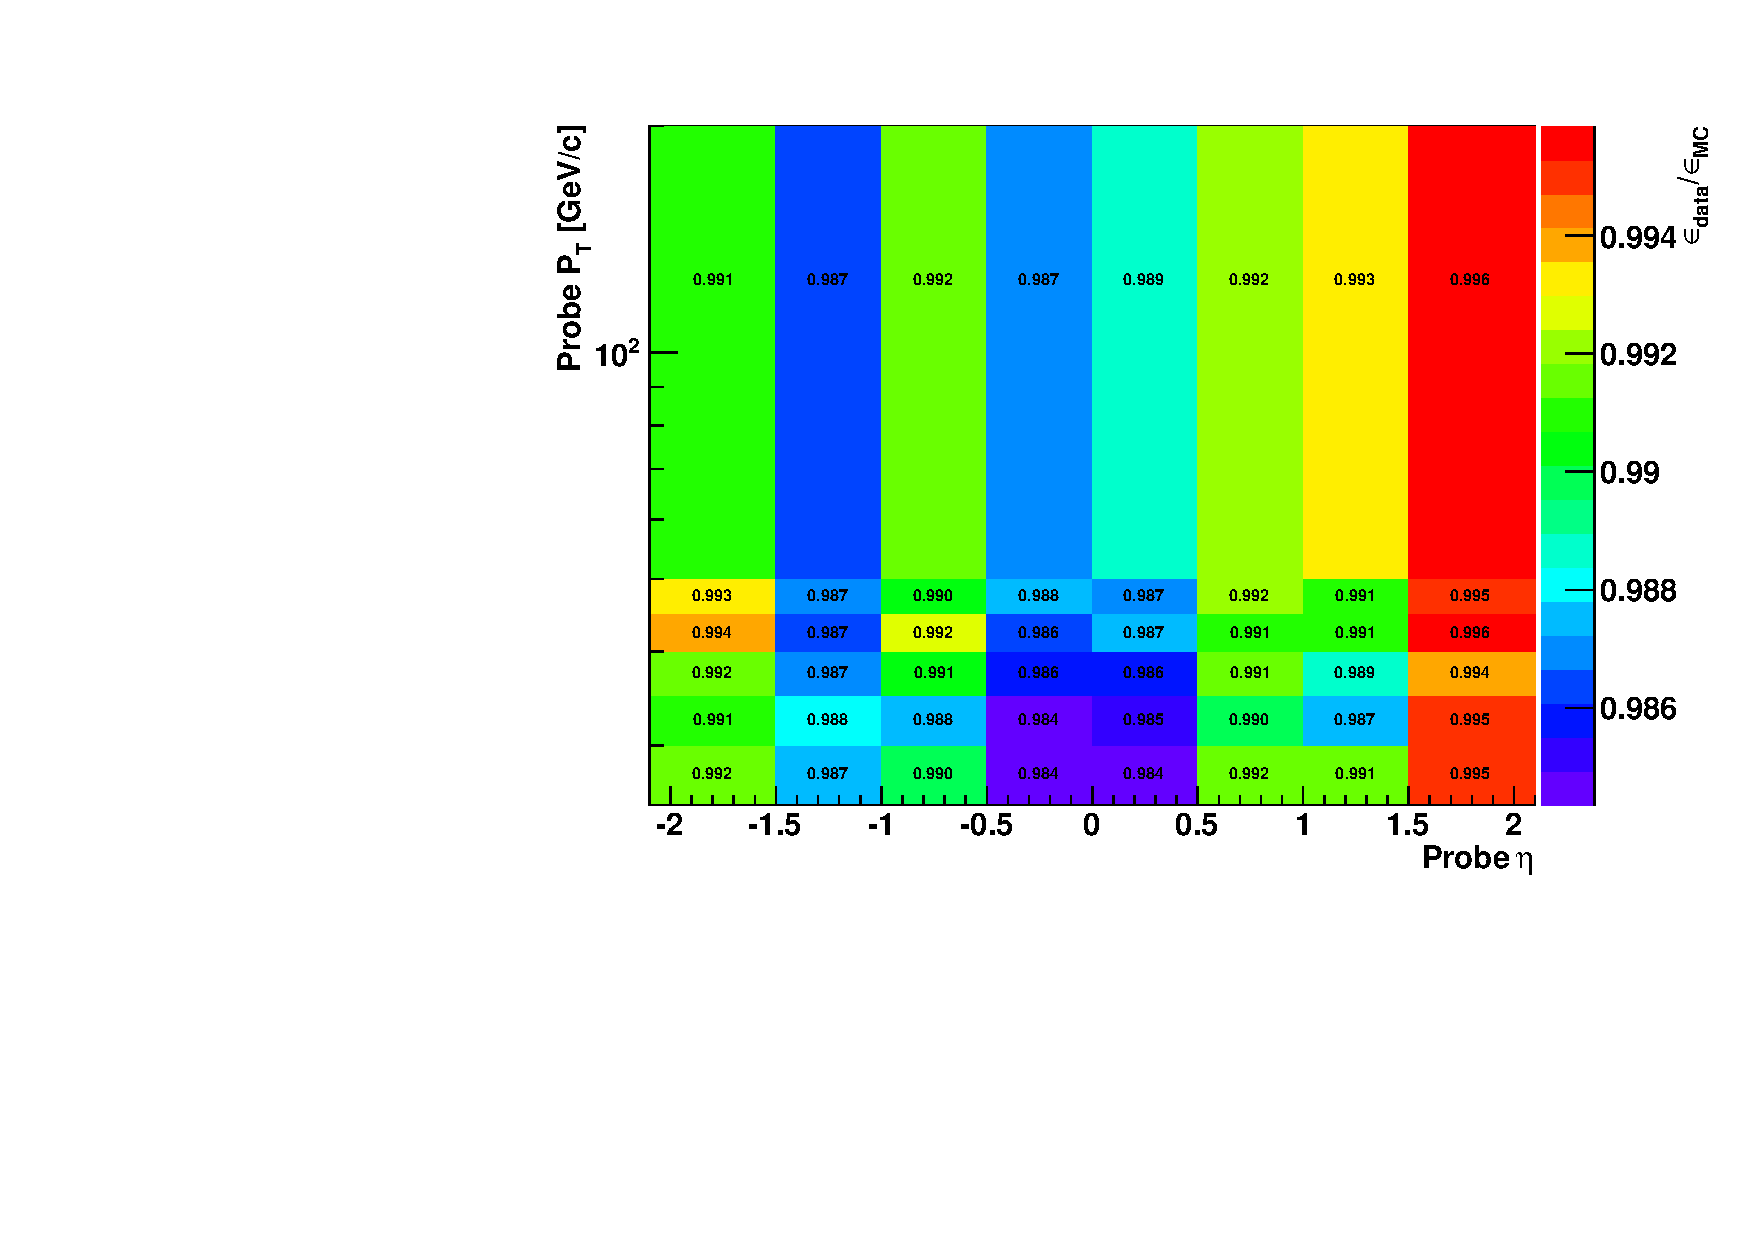
\includegraphics[width=0.47\textwidth]{figs/scaleFactor-Run2012ABC-RecoToIso.pdf}
  }
  \subfigure[]{
    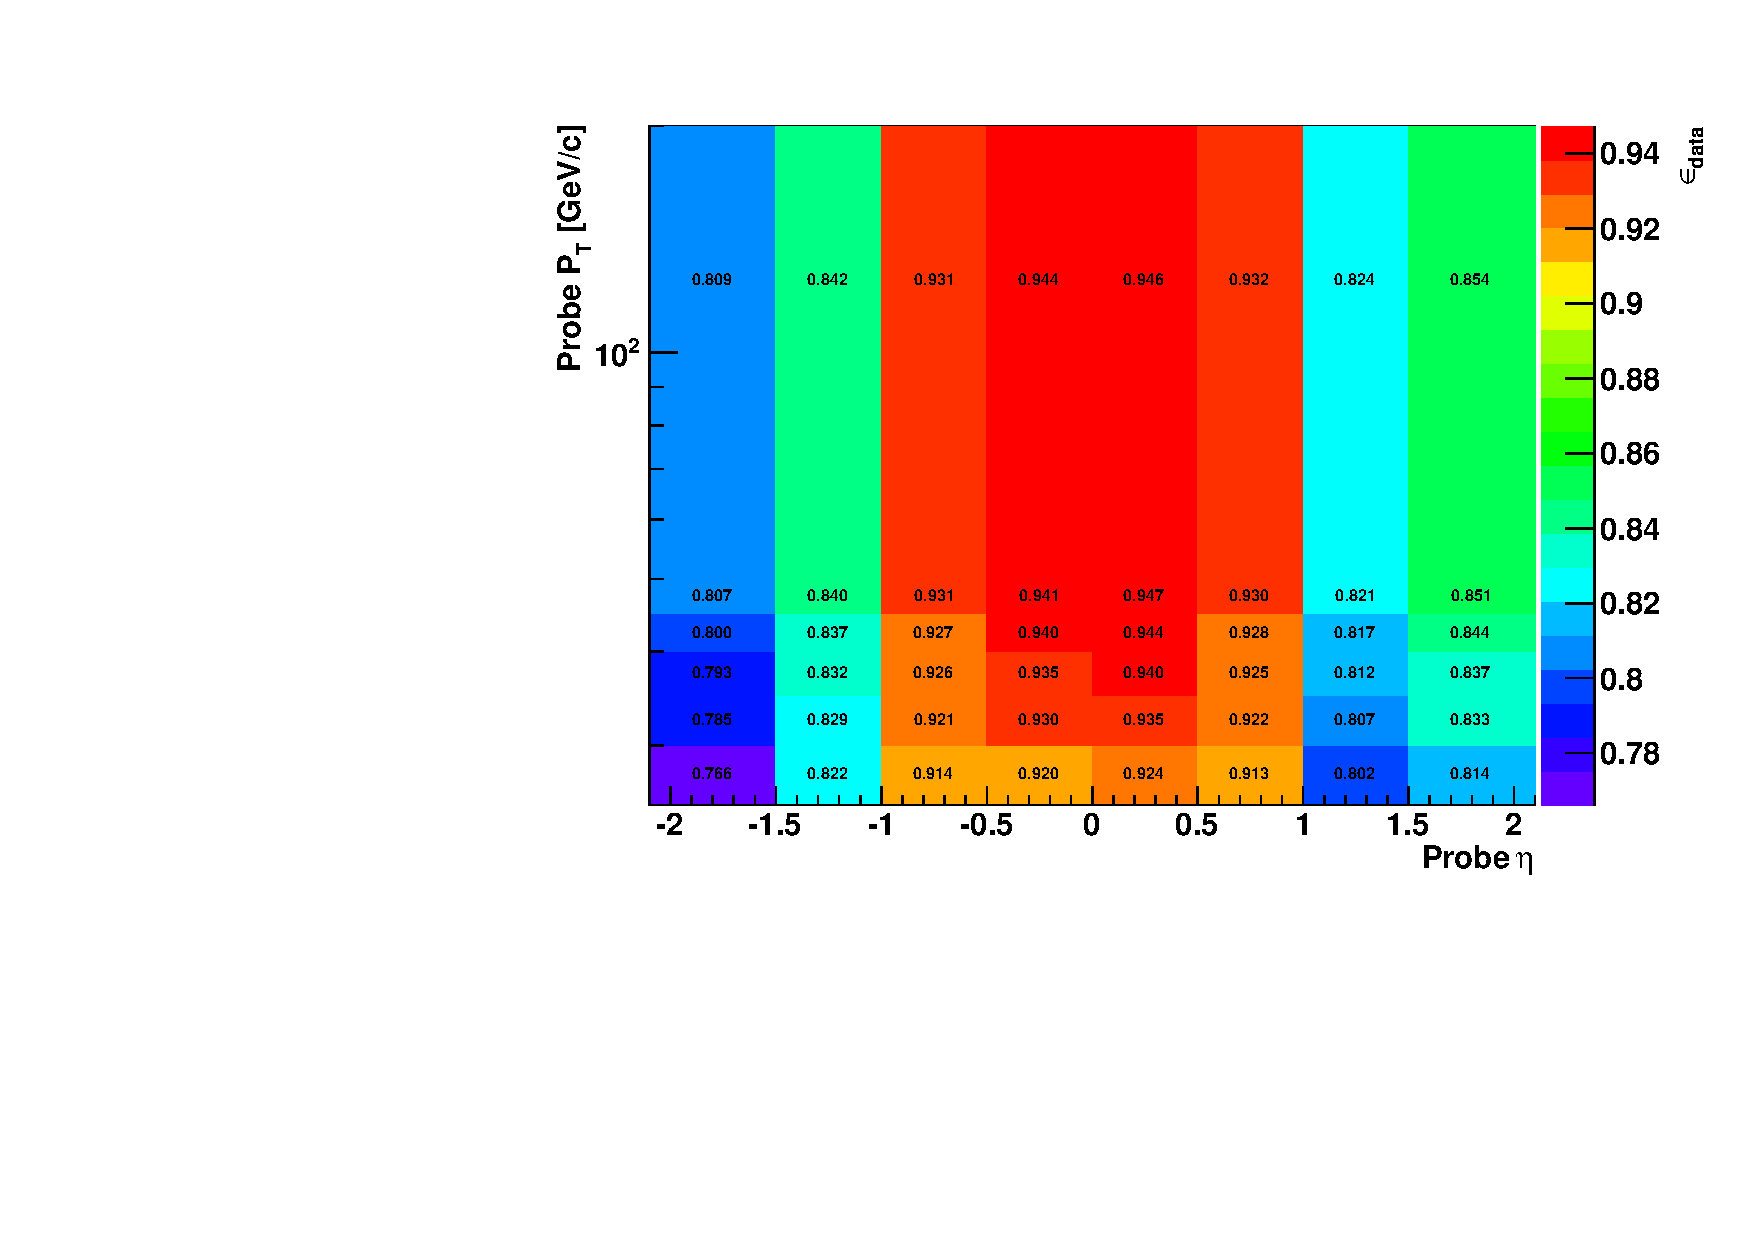
\includegraphics[width=0.47\textwidth]{figs/efficiency-Run2012ABC-IsoToIsoMuHLT.pdf}
  }
    \caption{Muon scale factors for reconstructed to selected muons $\epsilon_{\textnormal{ID,data}}$/$\epsilon_{\textnormal{ID,mc}}$ (a) and
    efficiency for selected to HLT muons $\epsilon_{\textnormal{HLT,data}}$ (b).}
    \label{fig:muonEff}
  \end{center}
\end{figure}



%%%%%%%%%%%%%%%%%%%%%%%%%%%%%%%%%%%%%%%%%%%%%%%%%%%%%%%%%%%%%%%%%%%%%%%%%%
%%%%%%%%%%%%%%%%%%%%%%%%%%%%%%%%%%%%%%%%%%%%%%%%%%%%%%%%%%%%%%%%%%%%%%%%%%
%%\clearpage{}
\subsection{Comparison of Data and Monte Carlo simulation}
To assess the quality of the modeling provided by the MC simulation we 
make comparisons between the MC shape normalized to the total
prediction for the background compared to the overall data
yield after applying the event selection criteria (except for b-tag requirement in the dijet case). 
For the resolved case we show the distributions of various kinematic
variables after applying all the selection cuts in 
Figures ~\ref{fig:mu_jet_pt}-\ref{fig:mu_dijet}
for the muon+jets sample and in 
Figures ~\ref{fig:elec_jet_pt}-\ref{fig:elec_dijet} for
the electron+jets sample. The $E_T,\eta$ as well as $W_{mT}$ distributions show some discrepancy between data and MC due to inadequate recoil modeling in W+Jets Monte Carlo, with the effect becoming more prevalent in higher jet bins. It is also more pronounced for electrons due to the fact that they are calorimeter objects and exhibit a higher degree of correlation with the jets.
Overall, there is reasonable agreement between data and simulation 
after analysis-level selection.
Although there are some notable differences in few places 
(\textit{e. g.}, in the jet $p_T$ spectra of Fig.~\ref{fig:mu_jet_pt} 
and Fig.~\ref{fig:elec_jet_pt} at high $p_T$ values),  
a part of the difference in each case 
is likely caused by the small size ($\approx 0.5 \times$ data)
of W+jets simulation sample. 
Seeing reasonable agreement gives us confidence in
the qualitative aspects of the MC modeling.

Likewise, we make comparisons of the data and MC for various kinematic observables for the merged selection. 
The distributions for the muon channel can be seen in Fig.~\ref{fig:control_boosted_mu}.
The distributions for the electron channel can be seen in Fig.~\ref{fig:control_boosted_el}.
In both the muon and electron cases, we find good agreement for the basic kinematic observables. It can also been seen that the dominant background contribution comes from the W+jets process with sub-leading contributions from 
the $t\bar{t}$ SM process and even smaller contributions from $WW/WZ$ and single $t$-quark processes. Control plots for the pruned jet mass and jet pT are provided in Fig.~\ref{fig:control_boosted_jet}. As can be seen, for the jet mass the data and MC distributions do not agree very well. This is known that the Pythia parton shower model does not do a good job of modeling the jet mass.  
It is known that the Herwig++ model does a slightly better job~\cite{SMPJS} though not with perfect agreement.  Thus, the resolution for the gaussian near the W and Z masses is corrected based on $t\bar{t}$ control sample studies (Section~\ref{sec:ttbar_merged}). Furthermore, we model the background shapes with parametric functions, with the parameters for the the dominant W+jets background (as well as the top falloff parameter) selected based on the data, and are able to model the data for the boosted topology (Section~\ref{sec:mjj_fit}).



%%%%%%%%%%%%%%%%%%%%%%%%%%%%
\begin{figure}[h!t]
  {\centering
    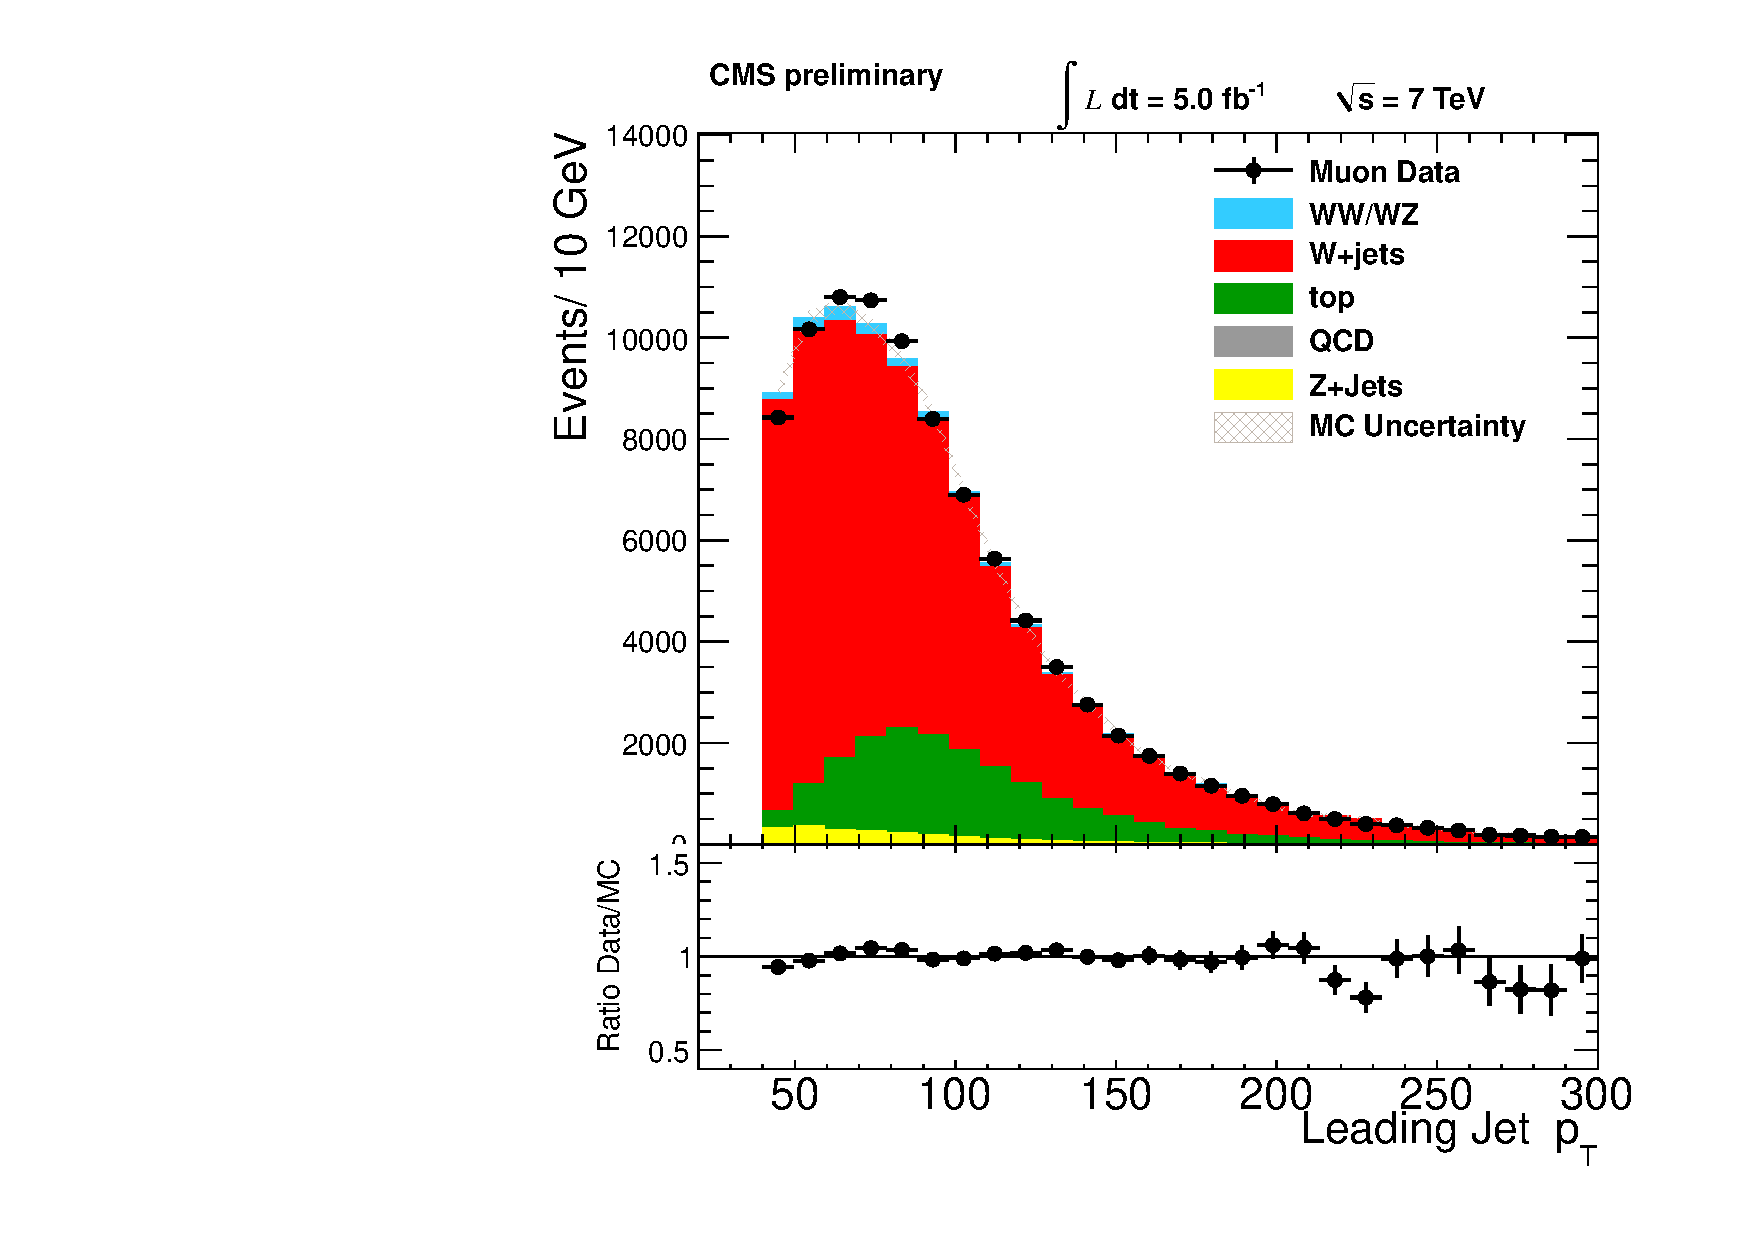
\includegraphics[width=0.49\textwidth]{figs/n-1_plots_mu/mu_jetld_pt.pdf}
    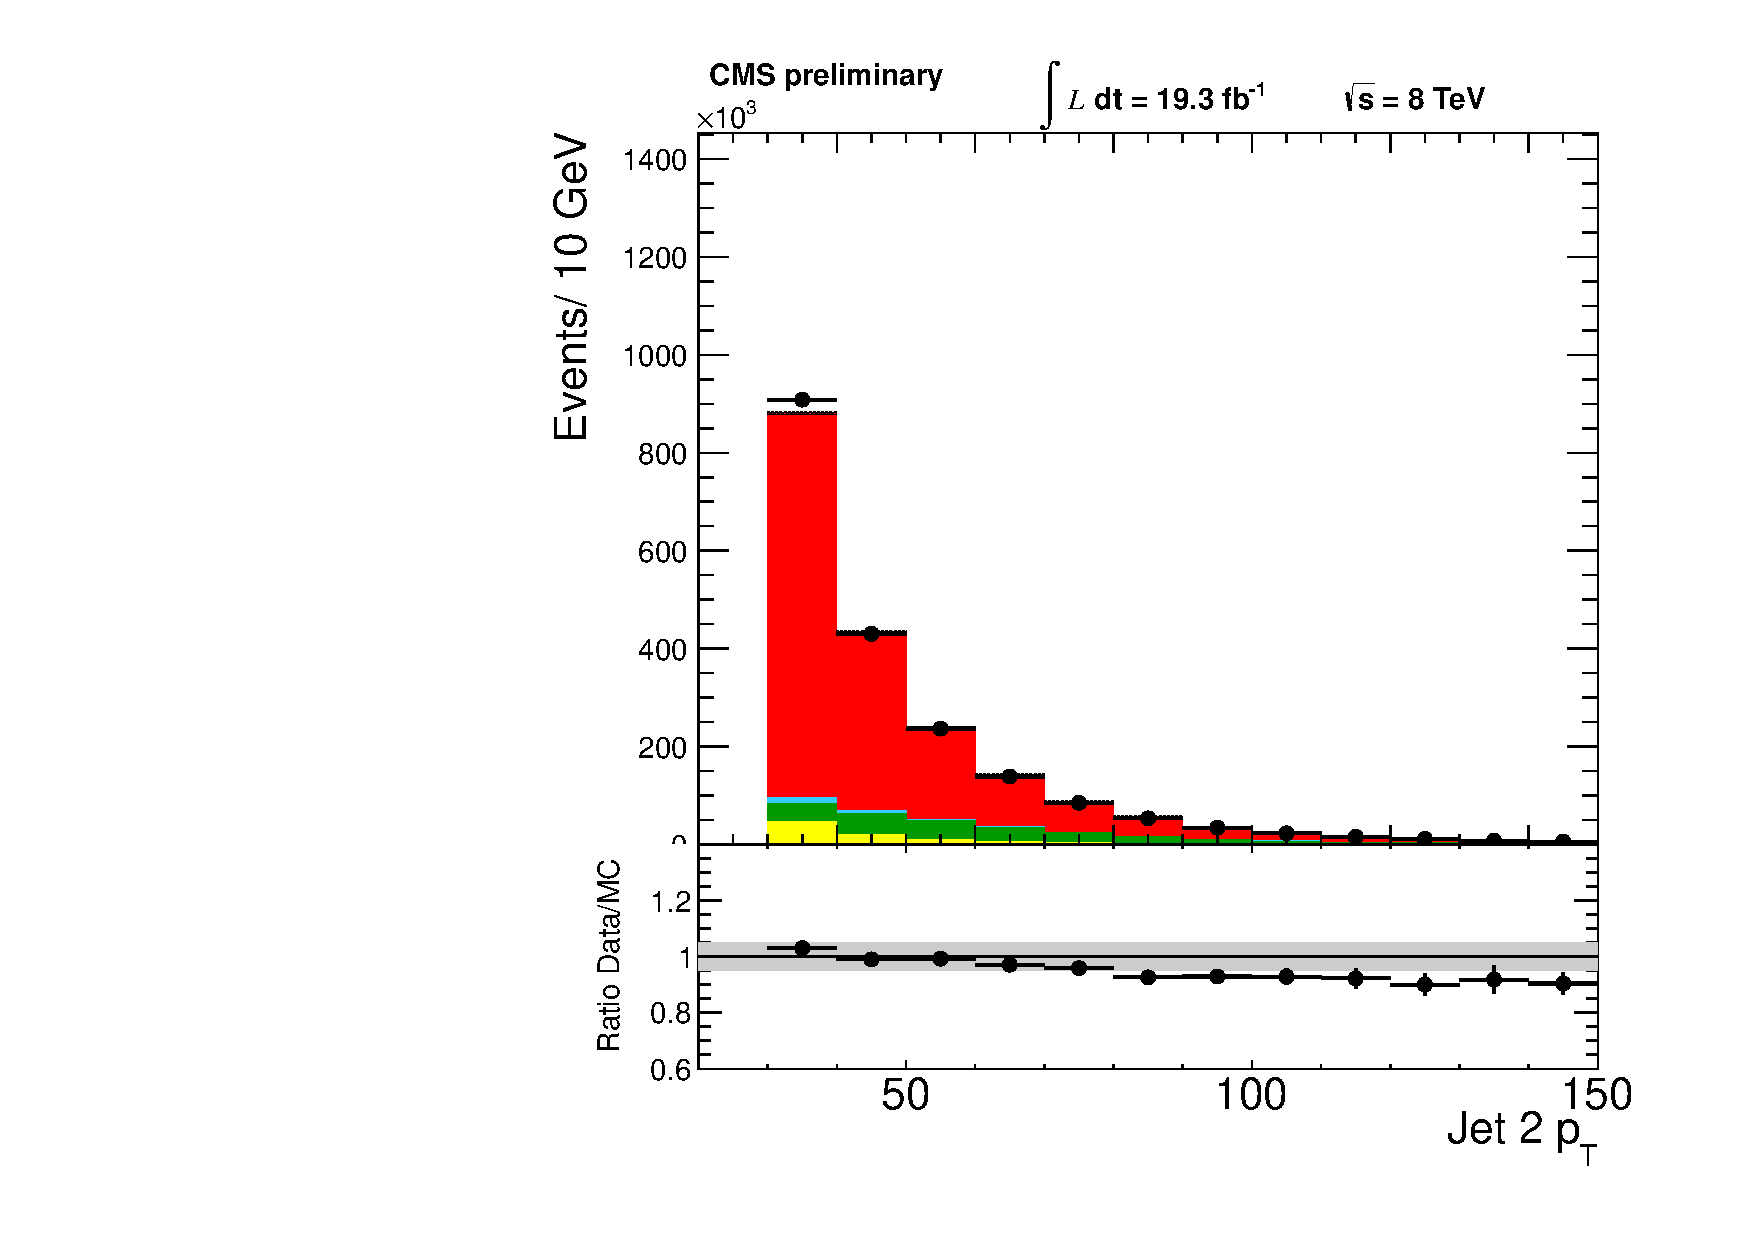
\includegraphics[width=0.49\textwidth]{figs/n-1_plots_mu/mu_jetnt_pt.pdf}
    \caption{Comparison of the leading jet (left) and 
      the second jet (right) $p_{T}$ distributions from data and MC for the muon+jets
      selection.}
    \label{fig:mu_jet_pt}}
\end{figure}
%%%%%%%%%%%%%%%%%%%%%%%%%%%%
\begin{figure}[h!t]
  {\centering
    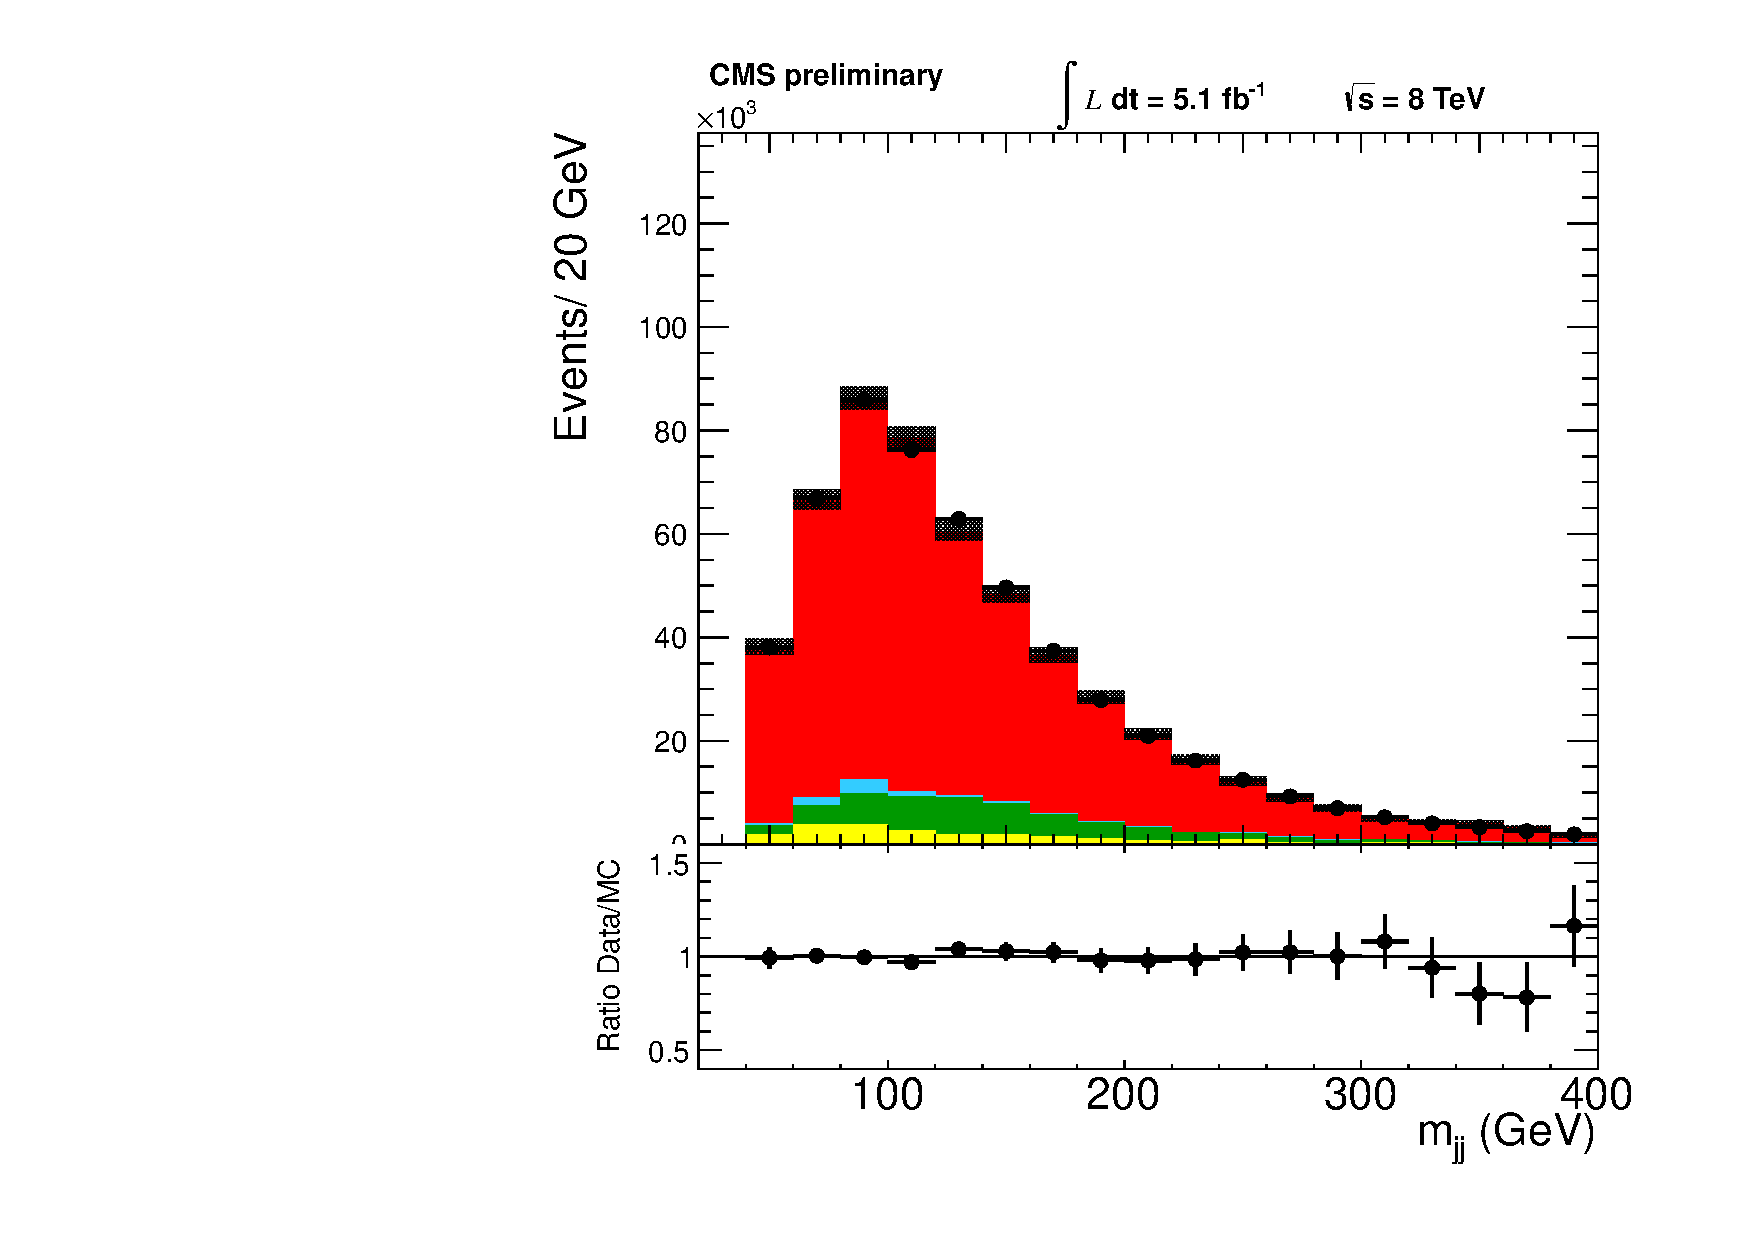
\includegraphics[width=0.49\textwidth]{figs/n-1_plots_mu/mu_mjj.pdf}
    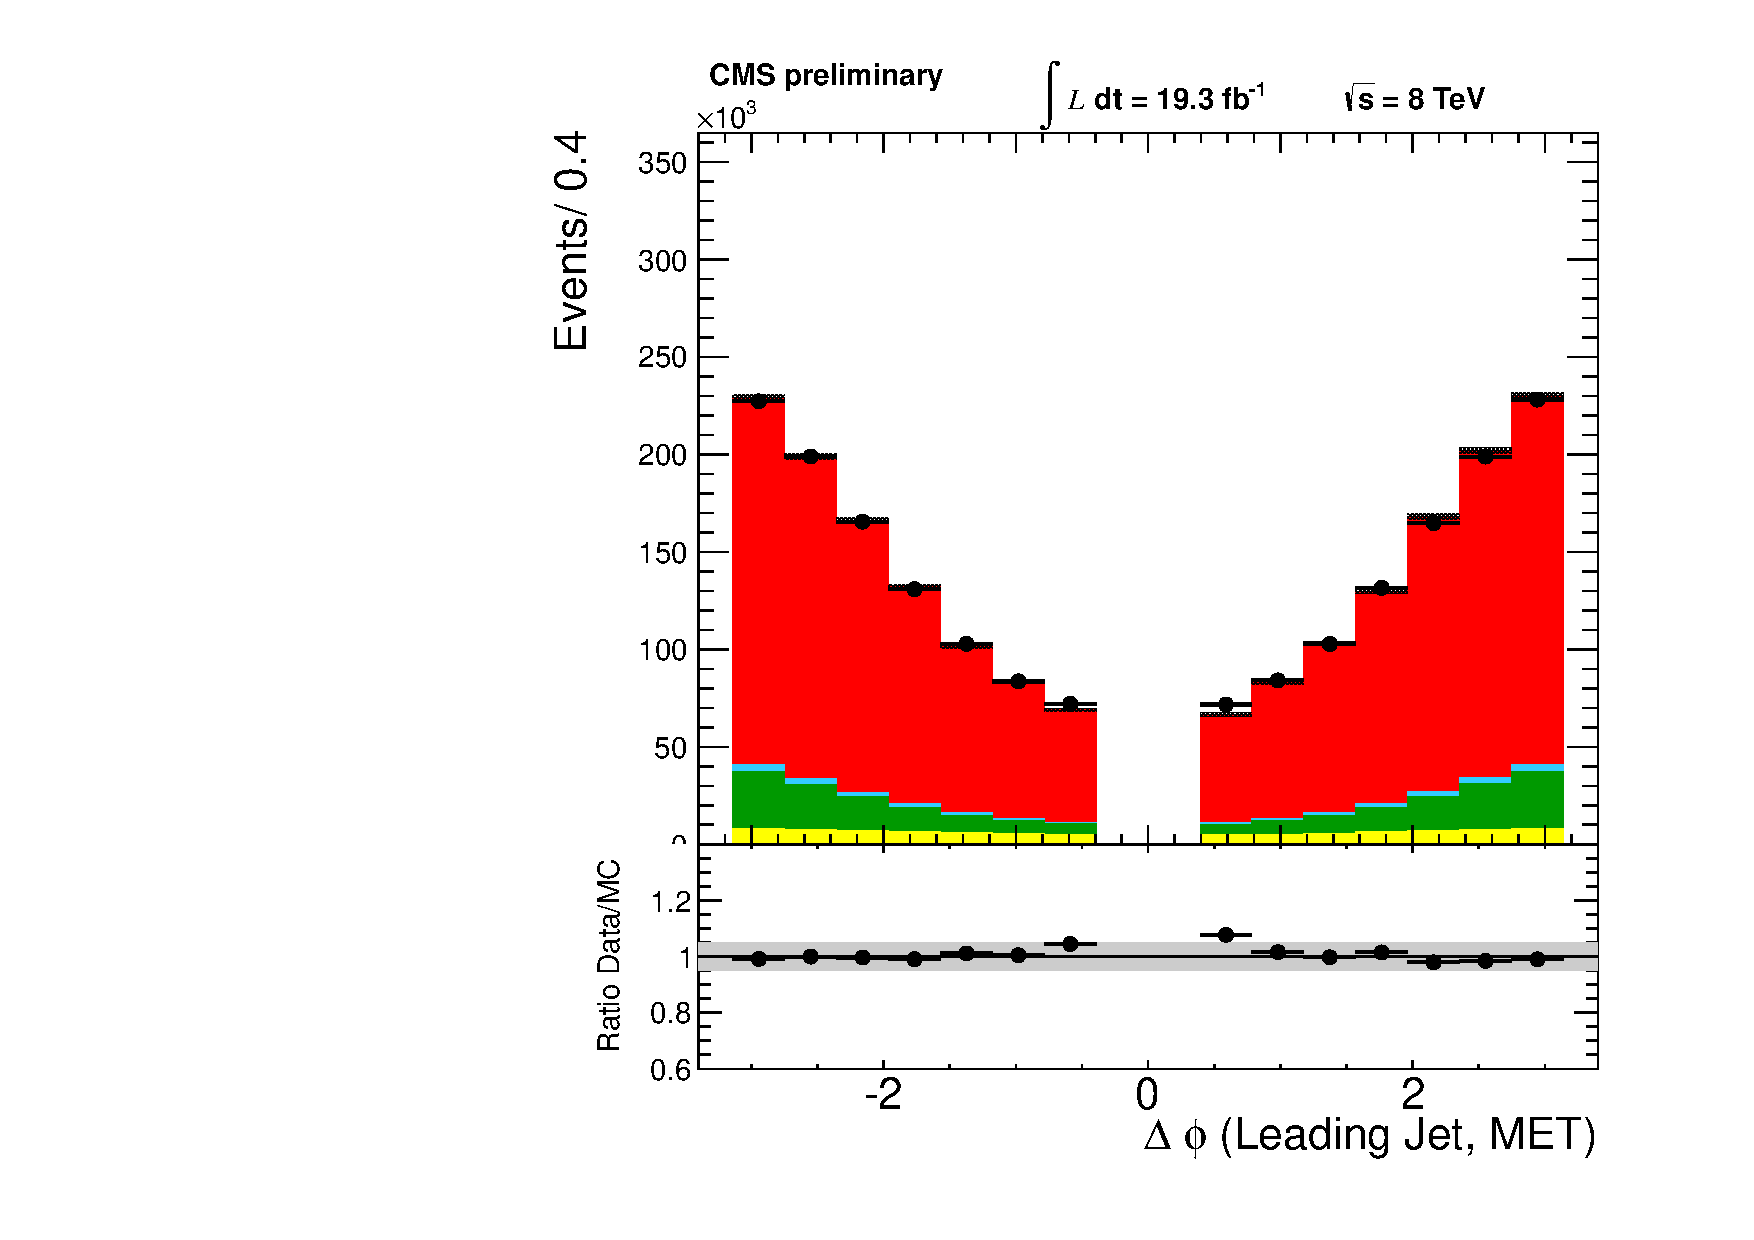
\includegraphics[width=0.49\textwidth]{figs/n-1_plots_mu/mu_deltaphi_jetldmet.pdf}
    \caption{Comparison of the distributions from data and MC of the
    dijet mass (left) and the $\Delta \phi $ between the leading jet and MET (right)
    for the muon+jets selection.}
\label{fig:mu_dijetmass}}
\end{figure}
\begin{figure}[h!t]
  {\centering
    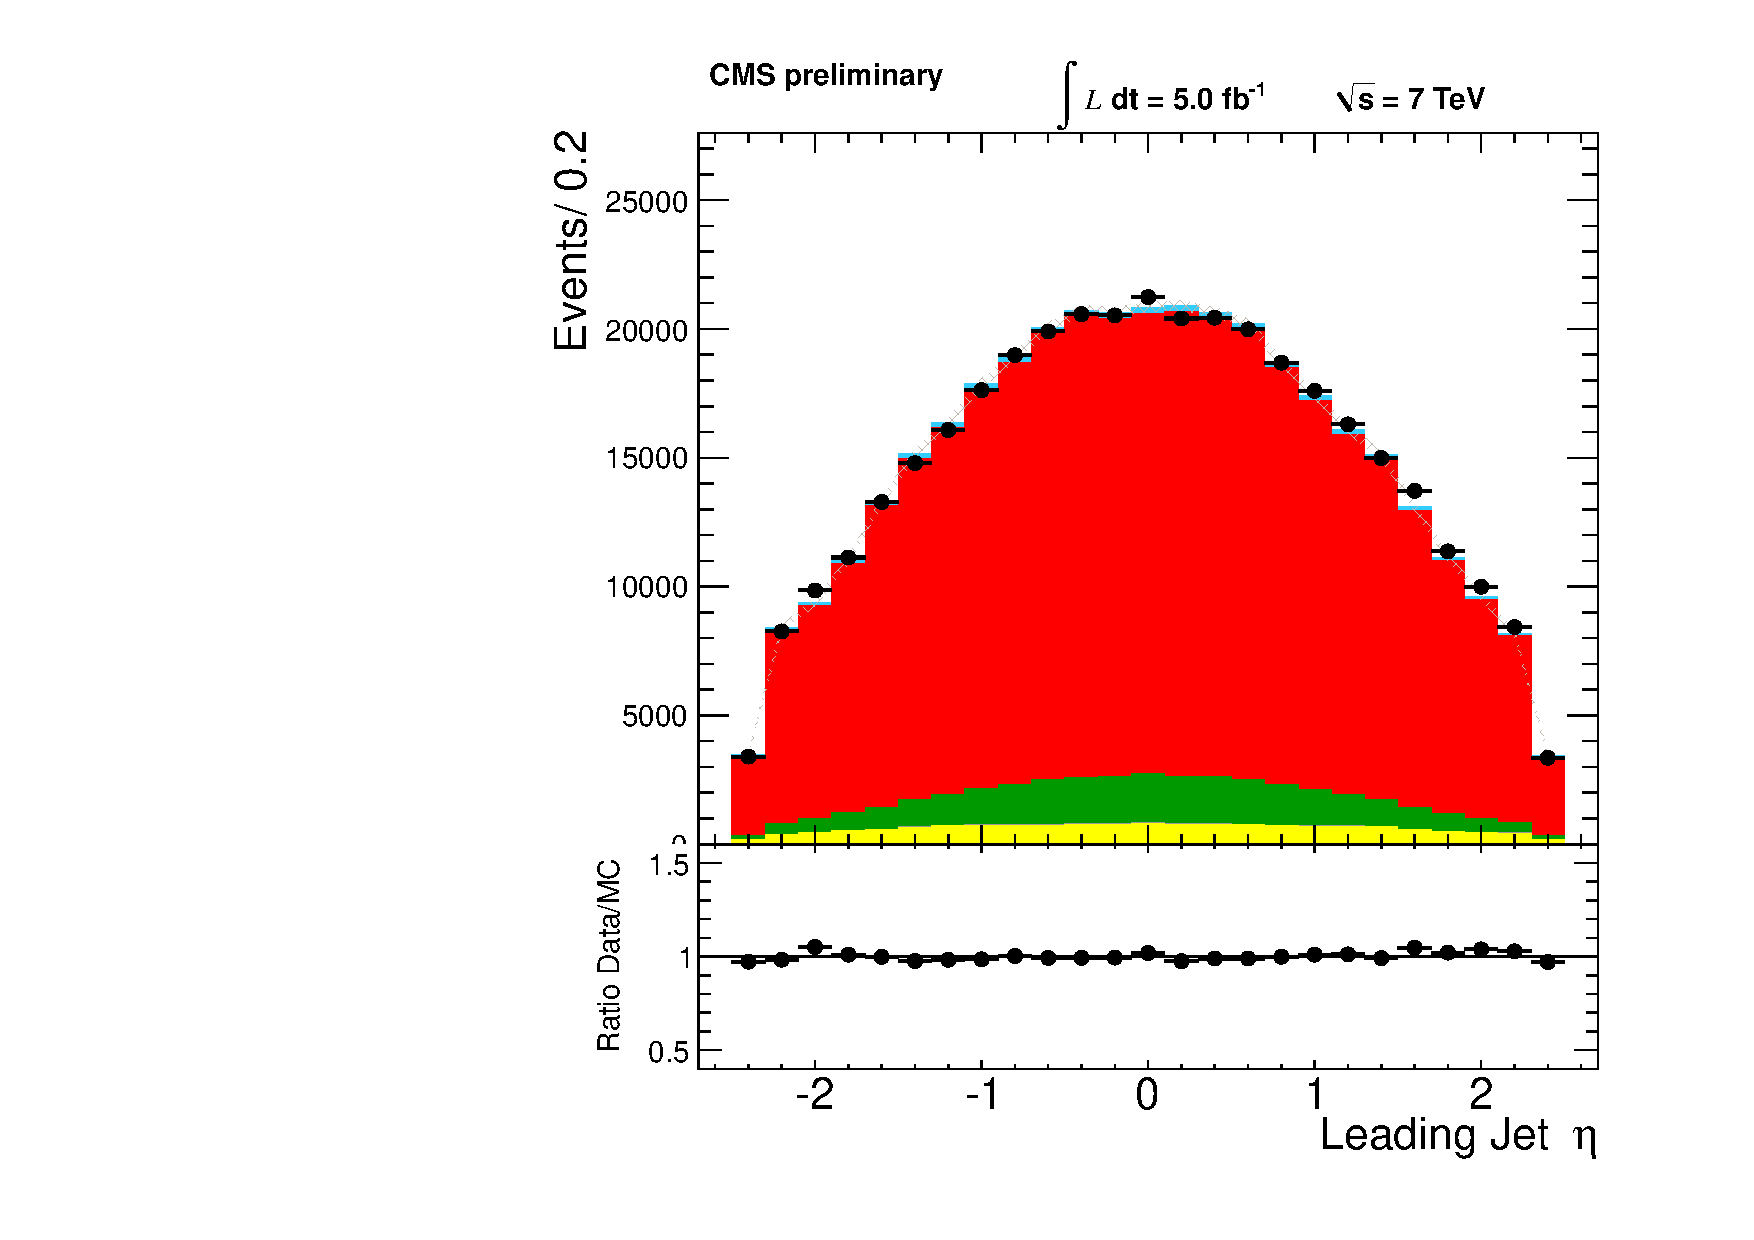
\includegraphics[width=0.49\textwidth]{figs/n-1_plots_mu/mu_jetld_eta.pdf}
    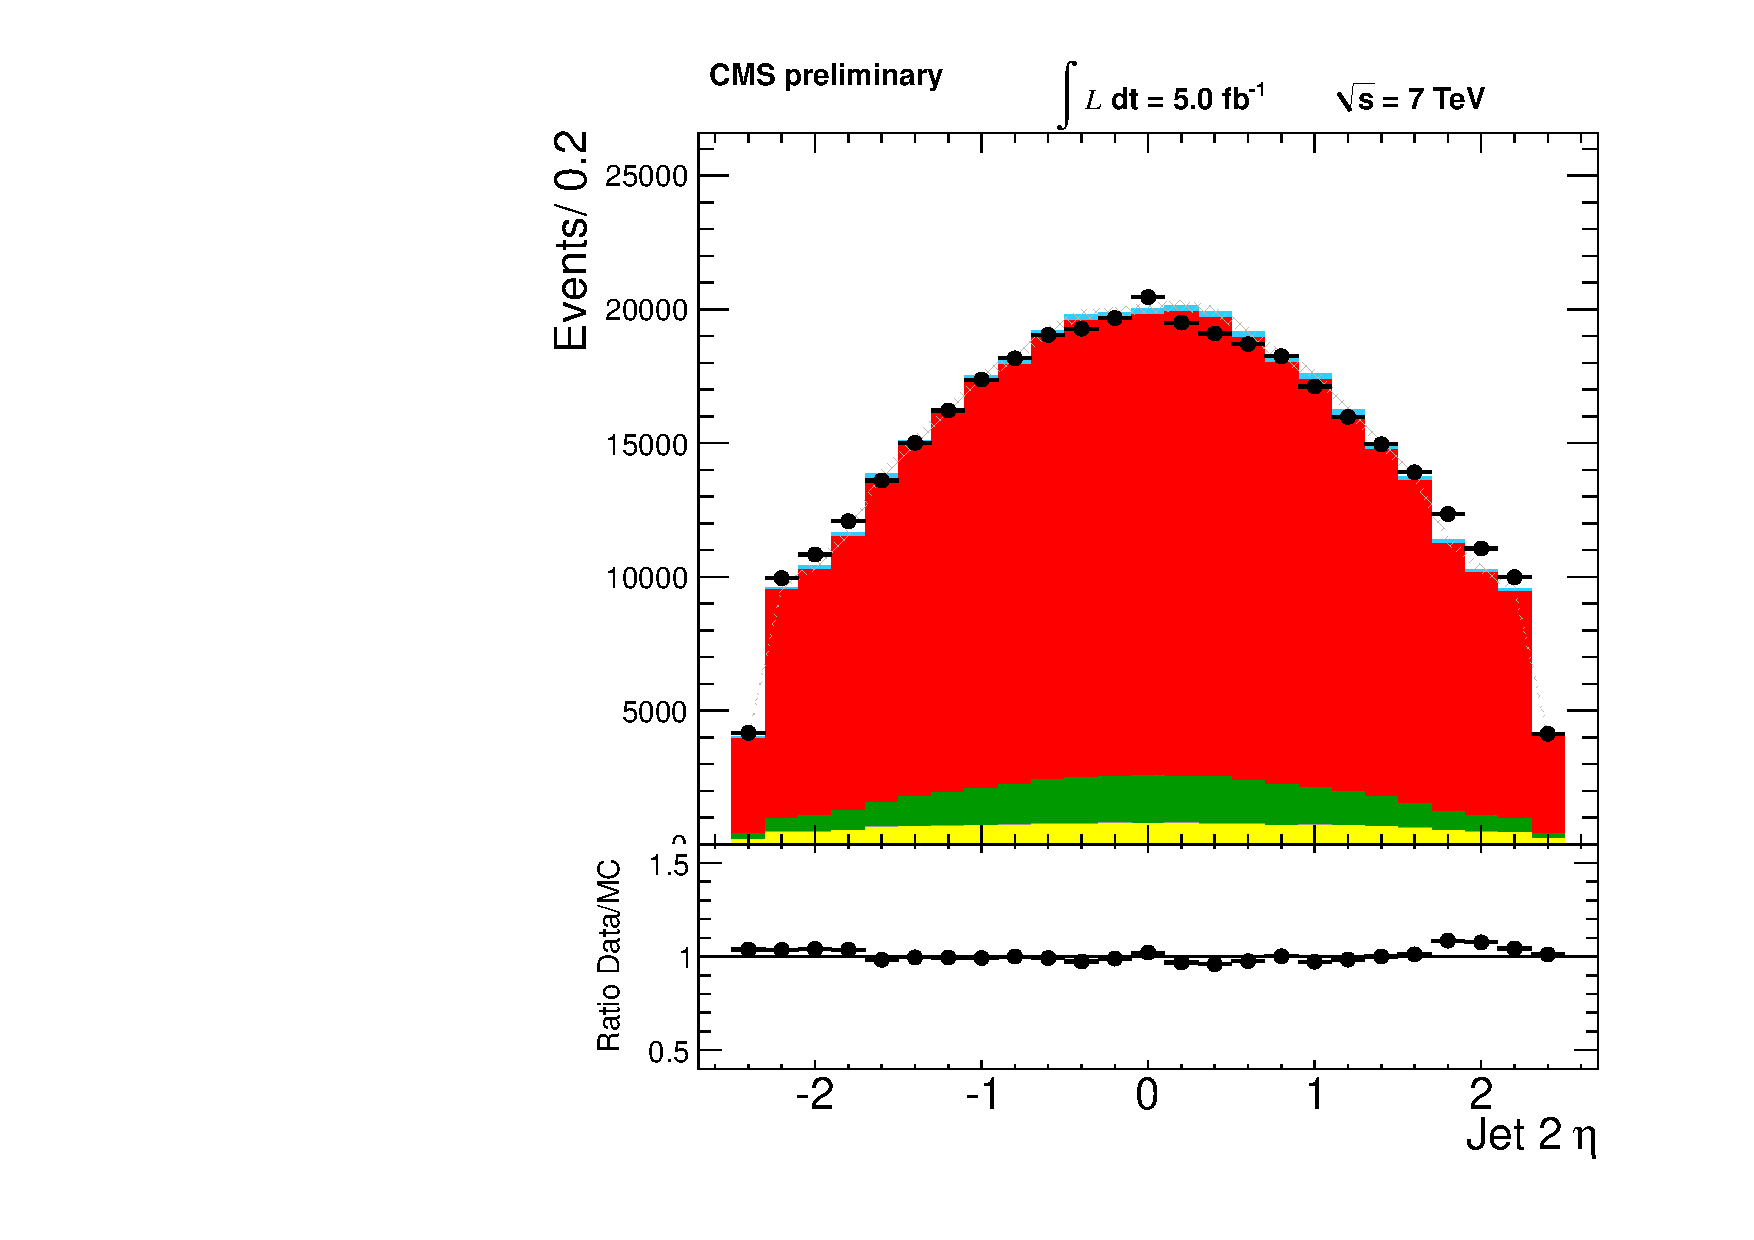
\includegraphics[width=0.49\textwidth]{figs/n-1_plots_mu/mu_jetnt_eta.pdf}
    \caption{Comparison of the leading jet $\eta $ (left) and the
    second leading jet $\eta $ (right) distributions from data and MC
    for the muon+jets selection. }
\label{fig:mu_jet_eta}}
\end{figure}
%%%%%%%%%%%%%%%%%%%%%%%%%%%%
\begin{figure}[h!t]
  {\centering
    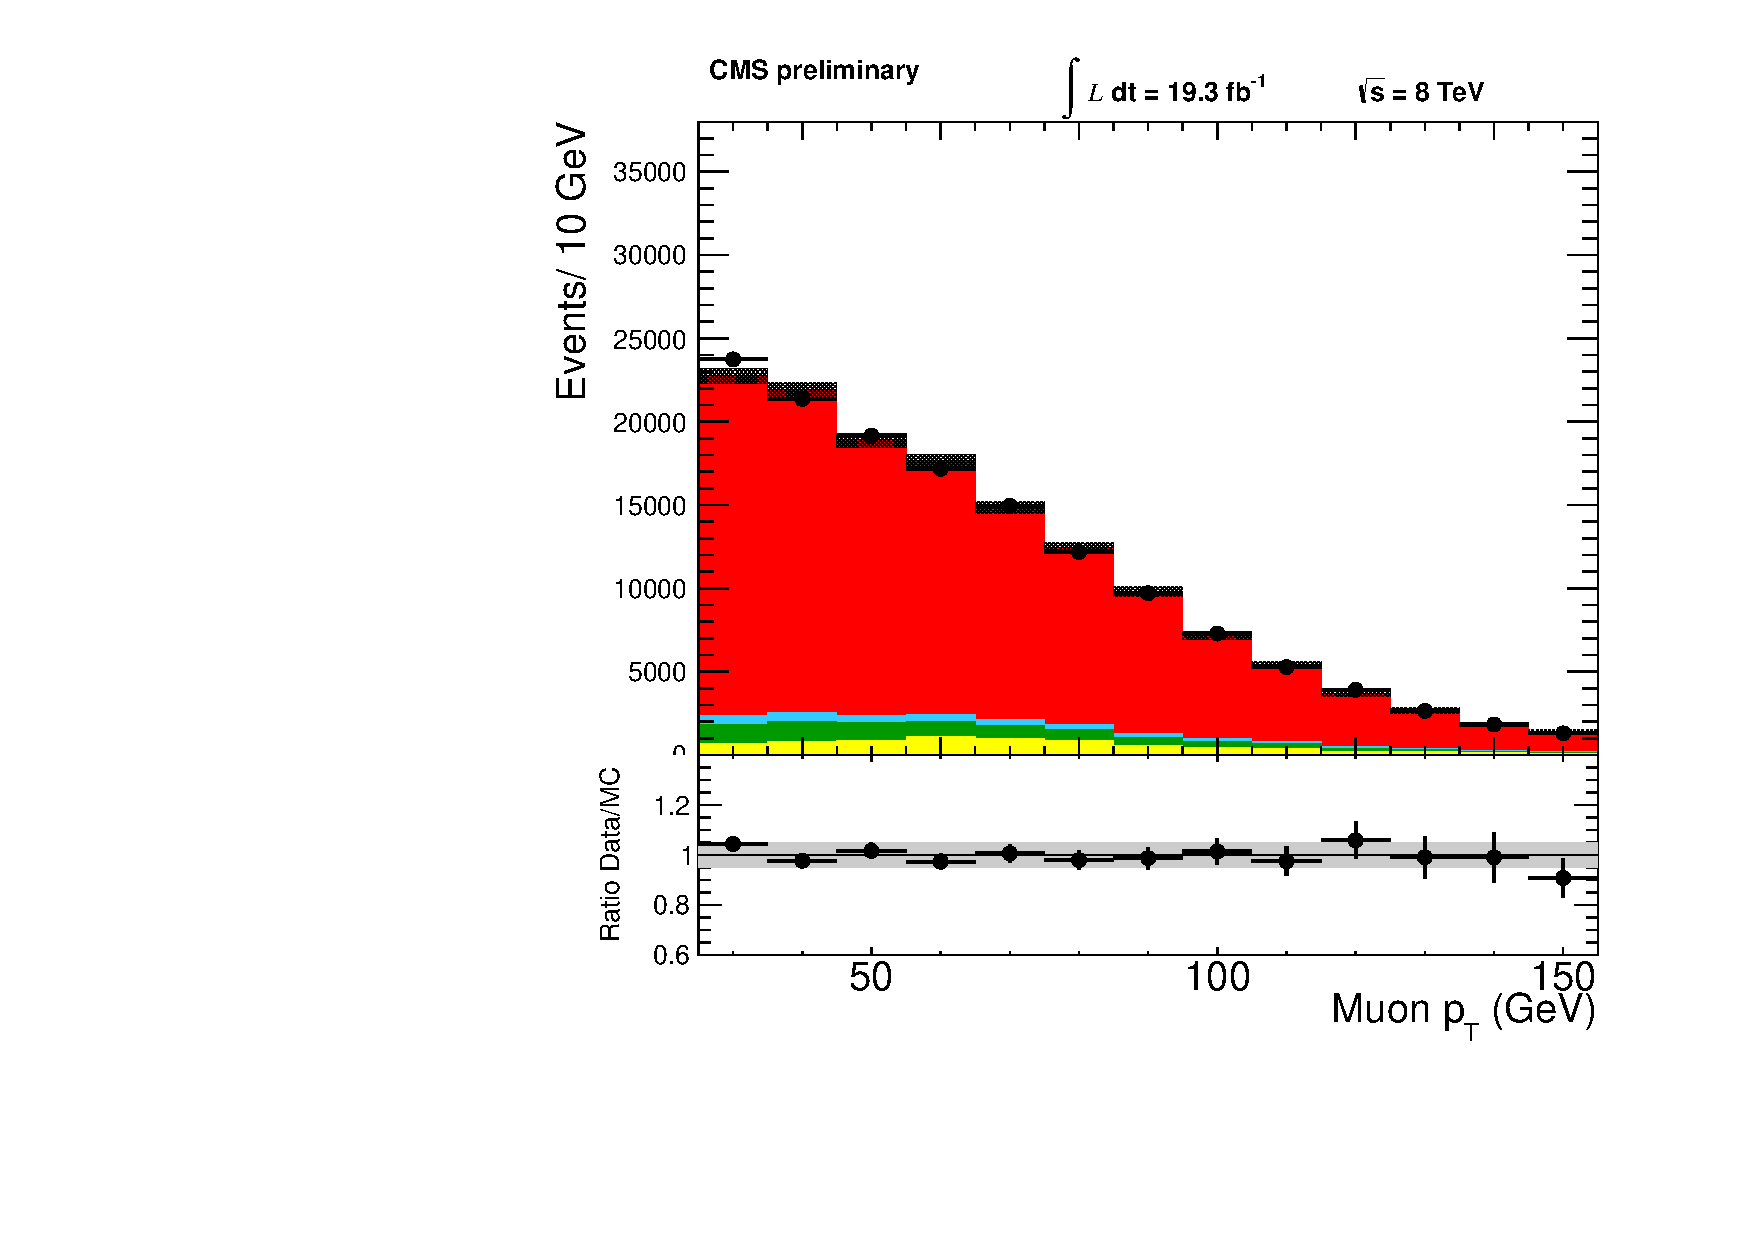
\includegraphics[width=0.49\textwidth]{figs/n-1_plots_mu/mu_W_muon_pt.pdf}
    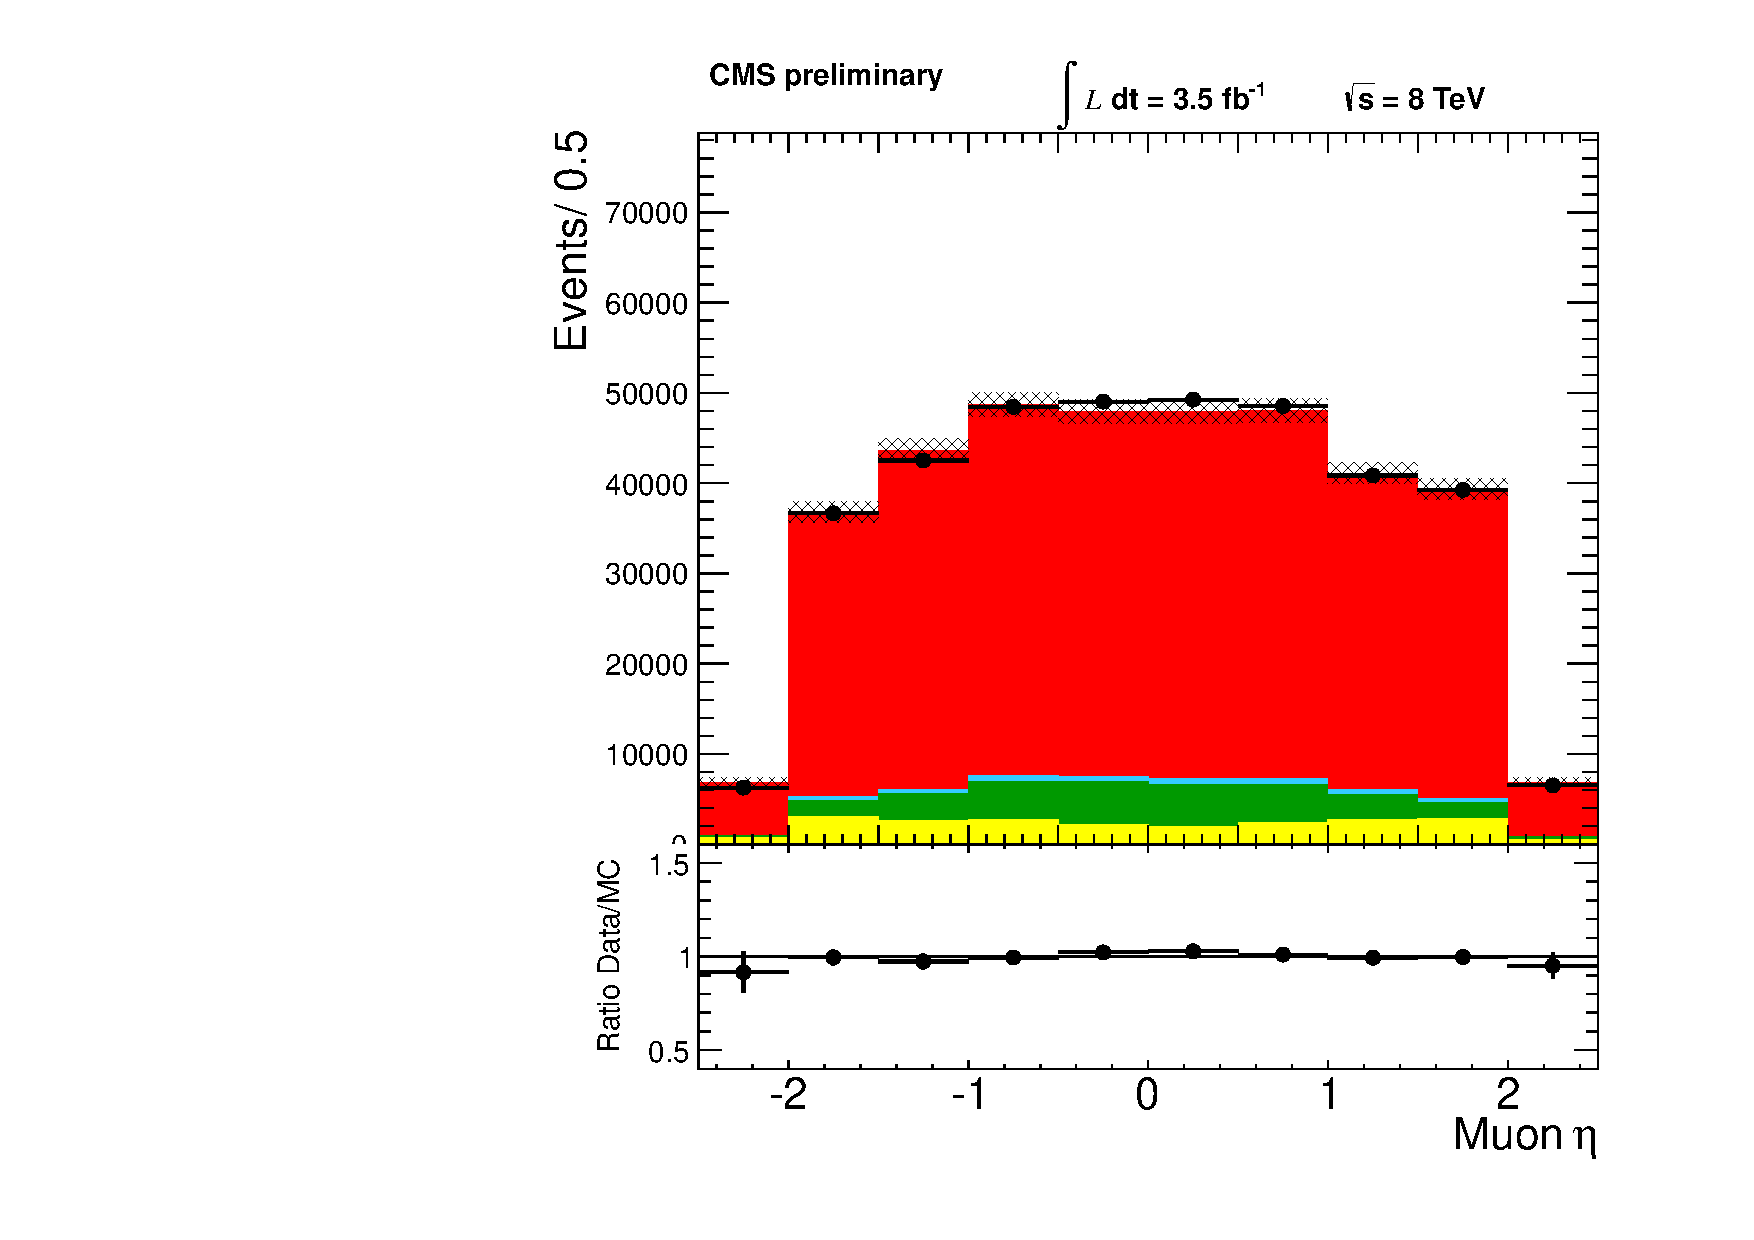
\includegraphics[width=0.49\textwidth]{figs/n-1_plots_mu/mu_W_muon_eta.pdf}
    \caption{Comparison of the muon $p_{T} $ (left) and the muon
      $\eta $ (right) distributions from data and MC for the muon+jets selection.
      }
    \label{fig:mu_muon}}
\end{figure}
%%%%%%%%%%%%%%%%%%%%%%%%%%%%
\begin{figure}[h!t]
  {\centering
    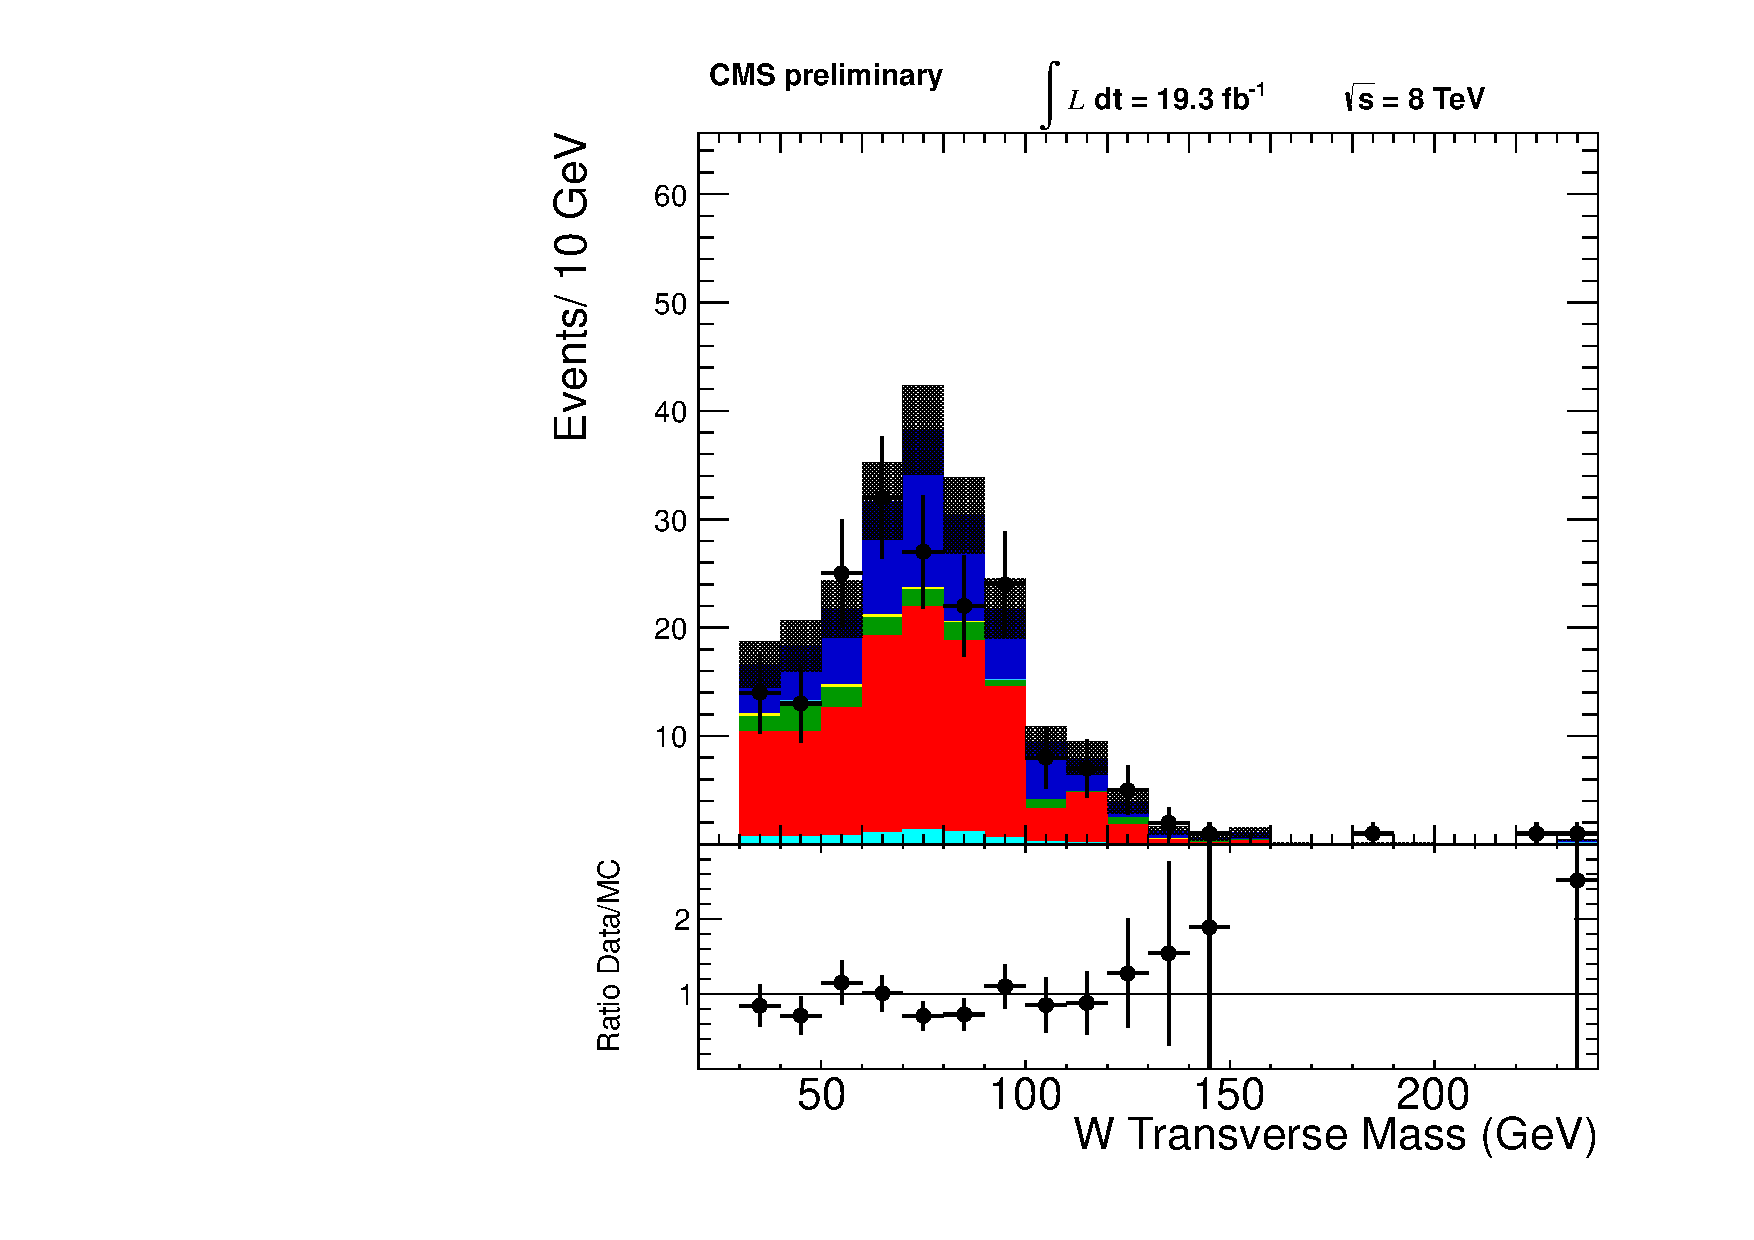
\includegraphics[width=0.49\textwidth]{figs/n-1_plots_mu/mu_W_mt.pdf}
    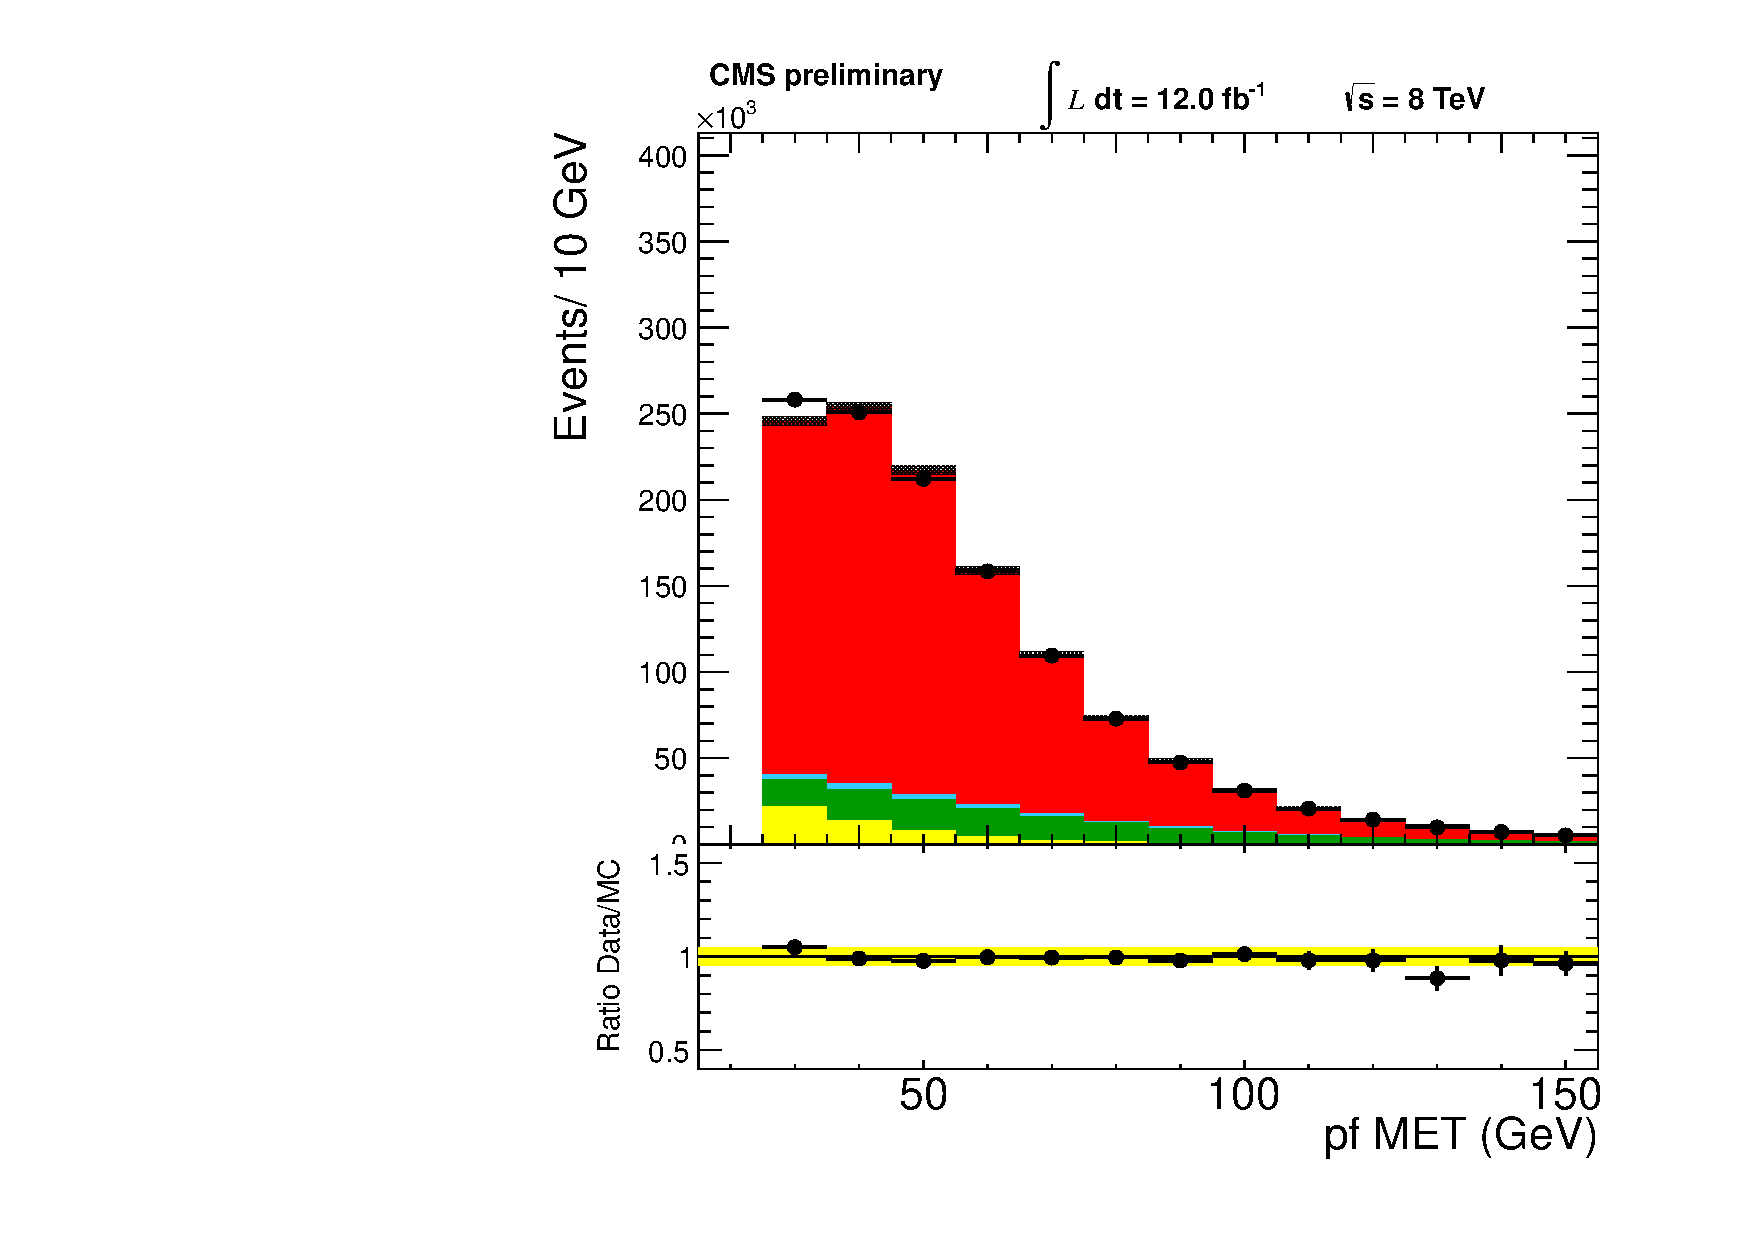
\includegraphics[width=0.49\textwidth]{figs/n-1_plots_mu/mu_event_met_pfmet.pdf}
    \caption{Comparison of the distributions from data and MC of the
     transverse mass of the muon / MET system (left) and the MET (right)
    for the muon+jets selection. 
    }
    \label{fig:mu_W_Mt}}
\end{figure}
%%%%%%%%%%%%%%%%%%%%%%%%%%%%
%%%%%%%%%%%%%%%%%%%%%%%%%%%%
\begin{figure}[h!t]
  {\centering
    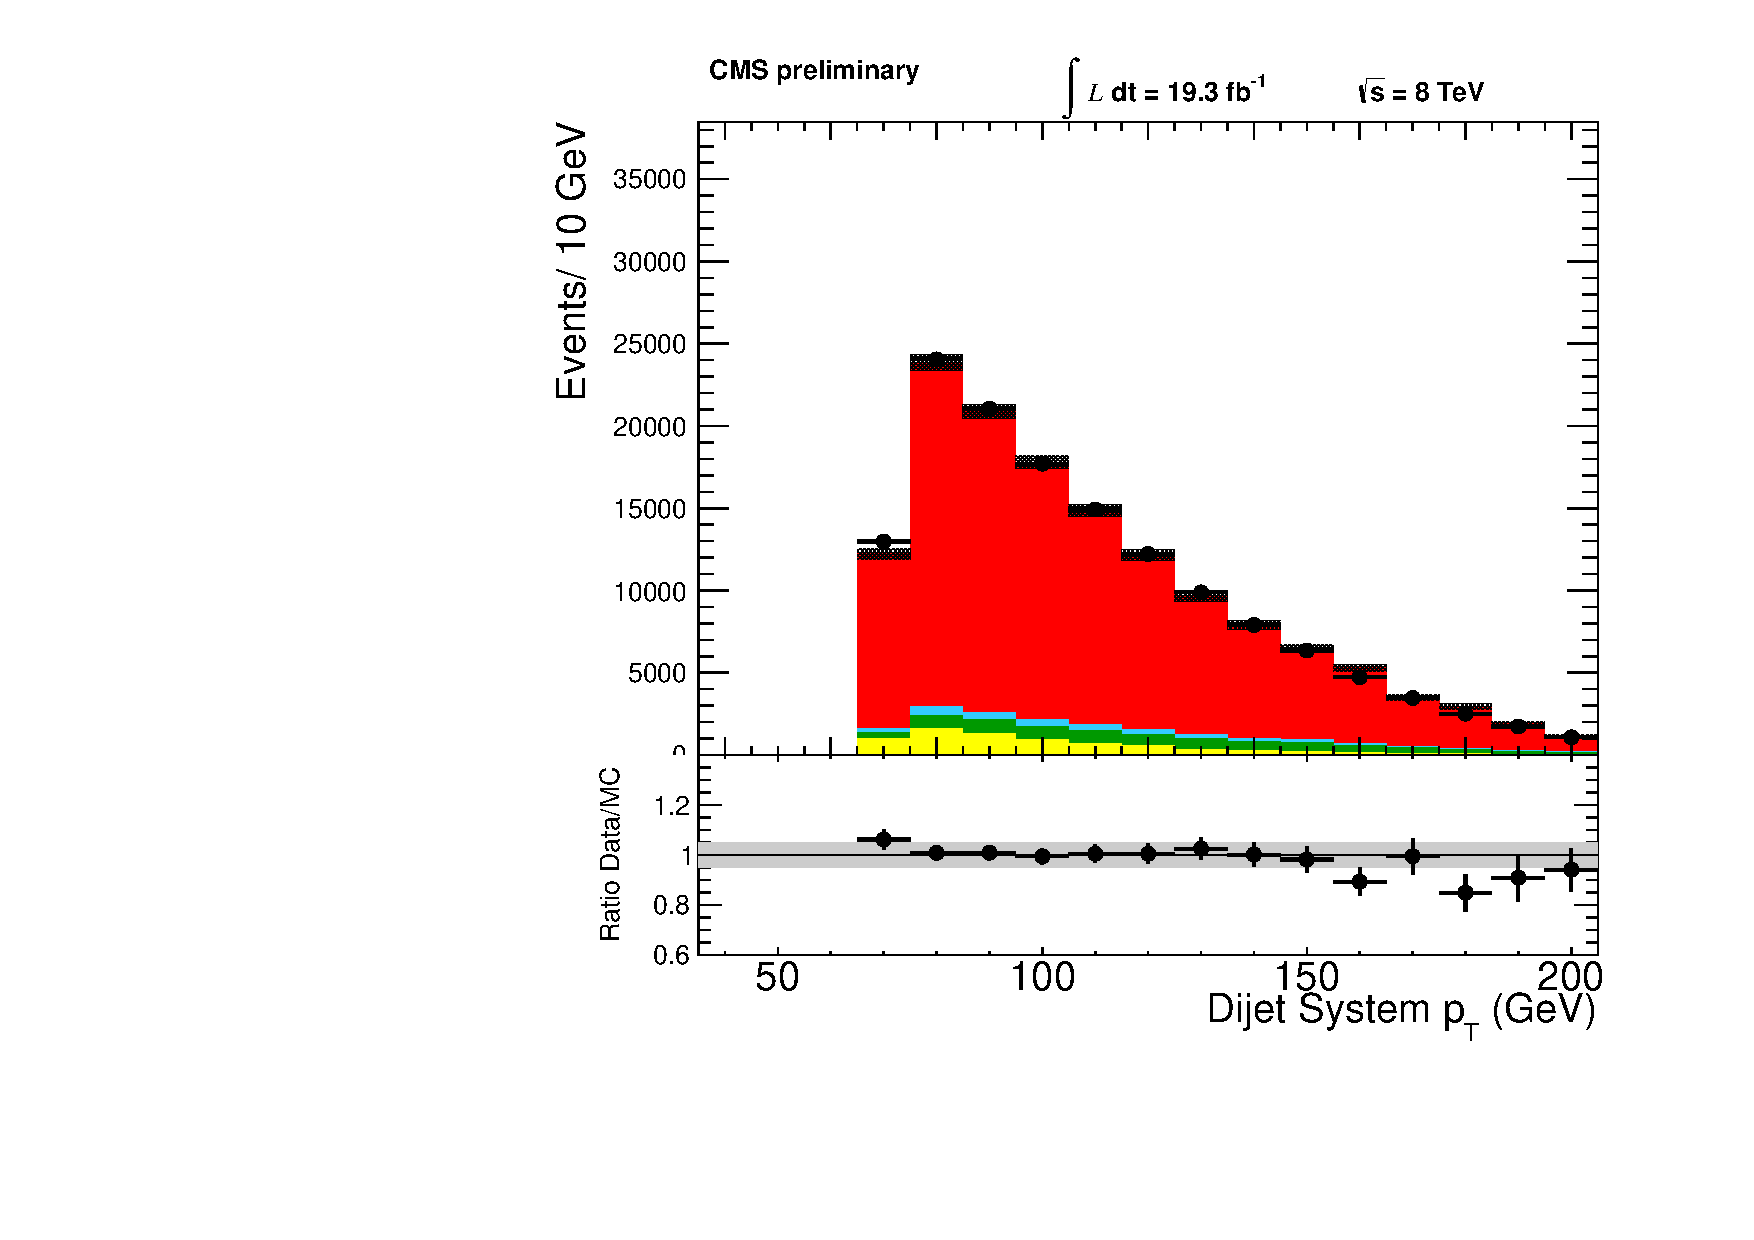
\includegraphics[width=0.49\textwidth]{figs/n-1_plots_mu/mu_dijet_pt.pdf}
    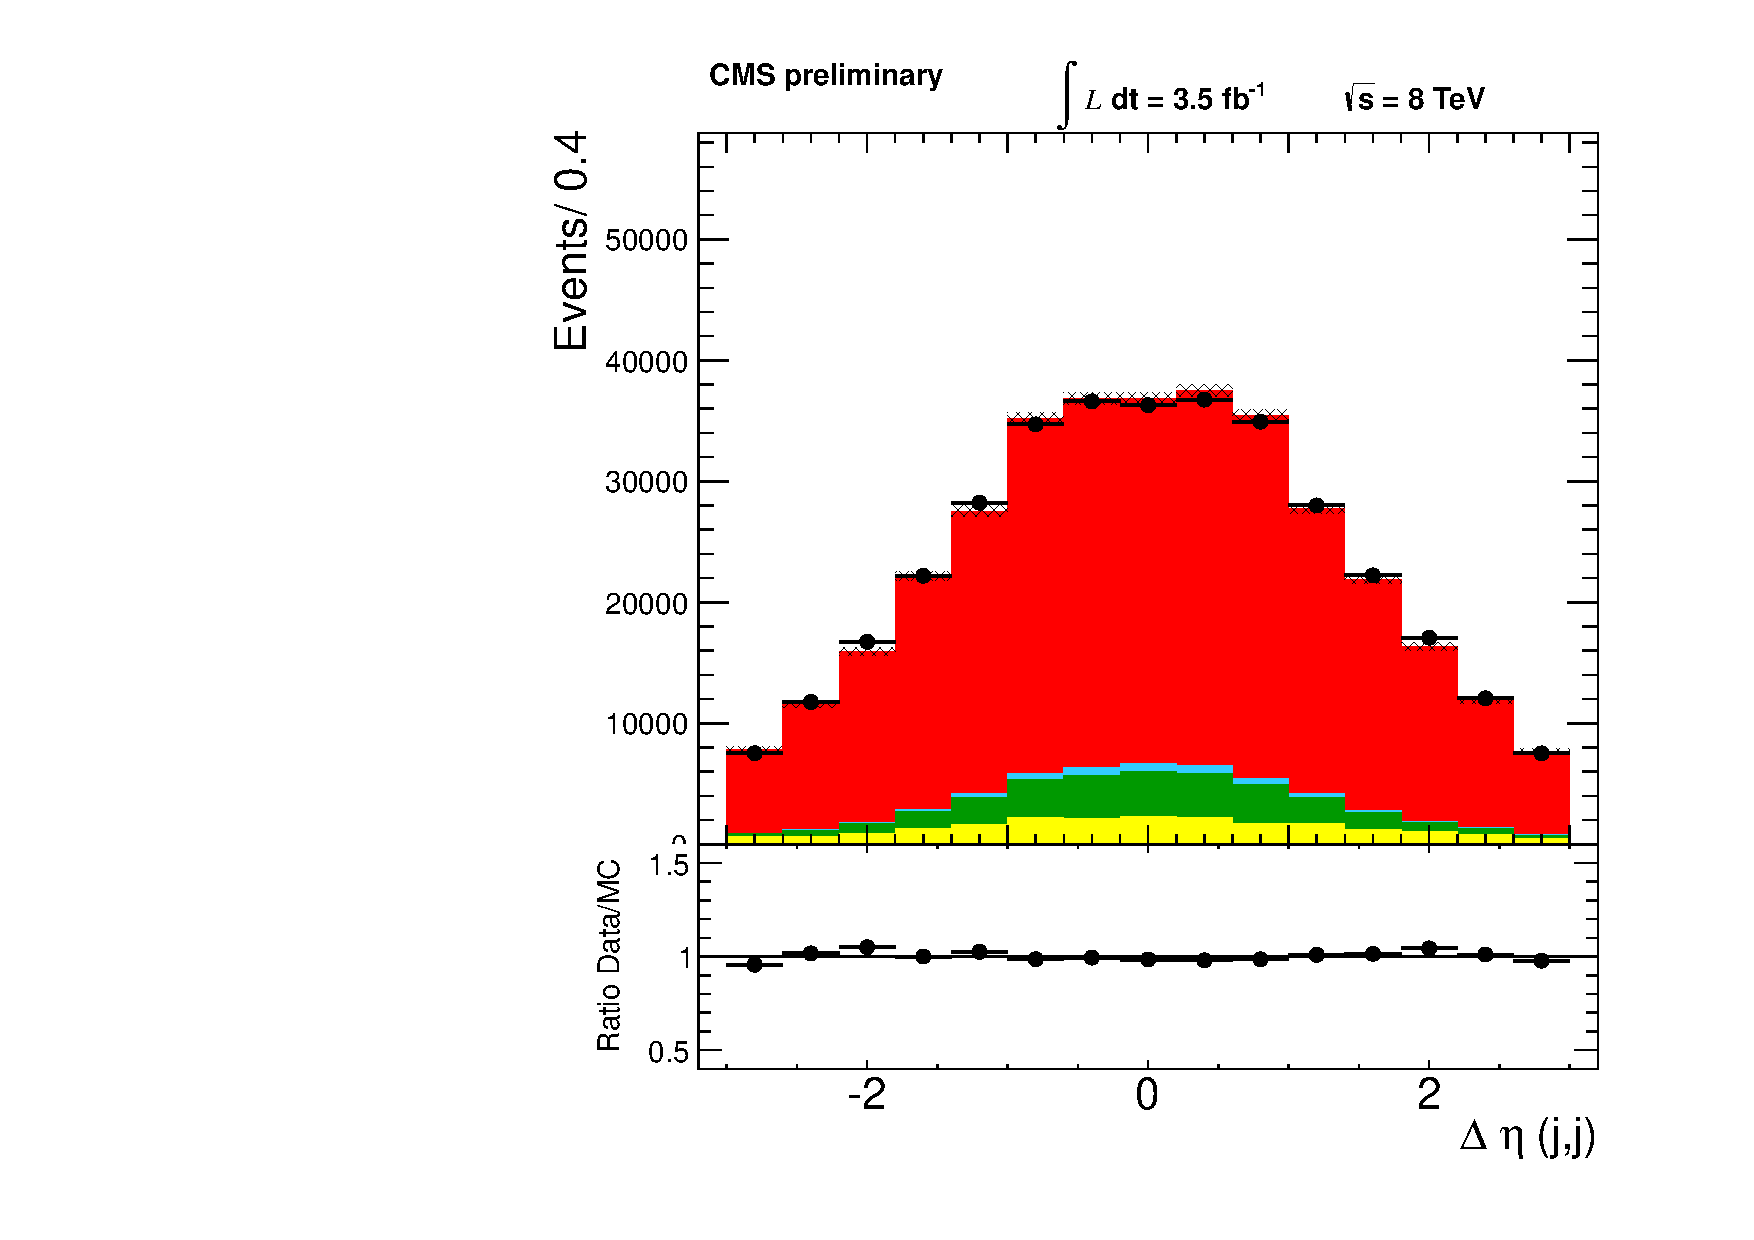
\includegraphics[width=0.49\textwidth]{figs/n-1_plots_mu/mu_deltaeta_jj.pdf}
    \caption{Comparison of the distributions from
      data and MC of the dijet system $p_{T}$ (left)
      and the $\eta $ separation between the two jets (right) for the muon+jets selection. 
      }
    \label{fig:mu_dijet}}
\end{figure}
%%%%%%%%%%%%%%%%%%%%%%%%%%%%
%%%%%%%%%%%%%%%%%%%%%%%%%%%%
\begin{figure}[h!t]
  {\centering
    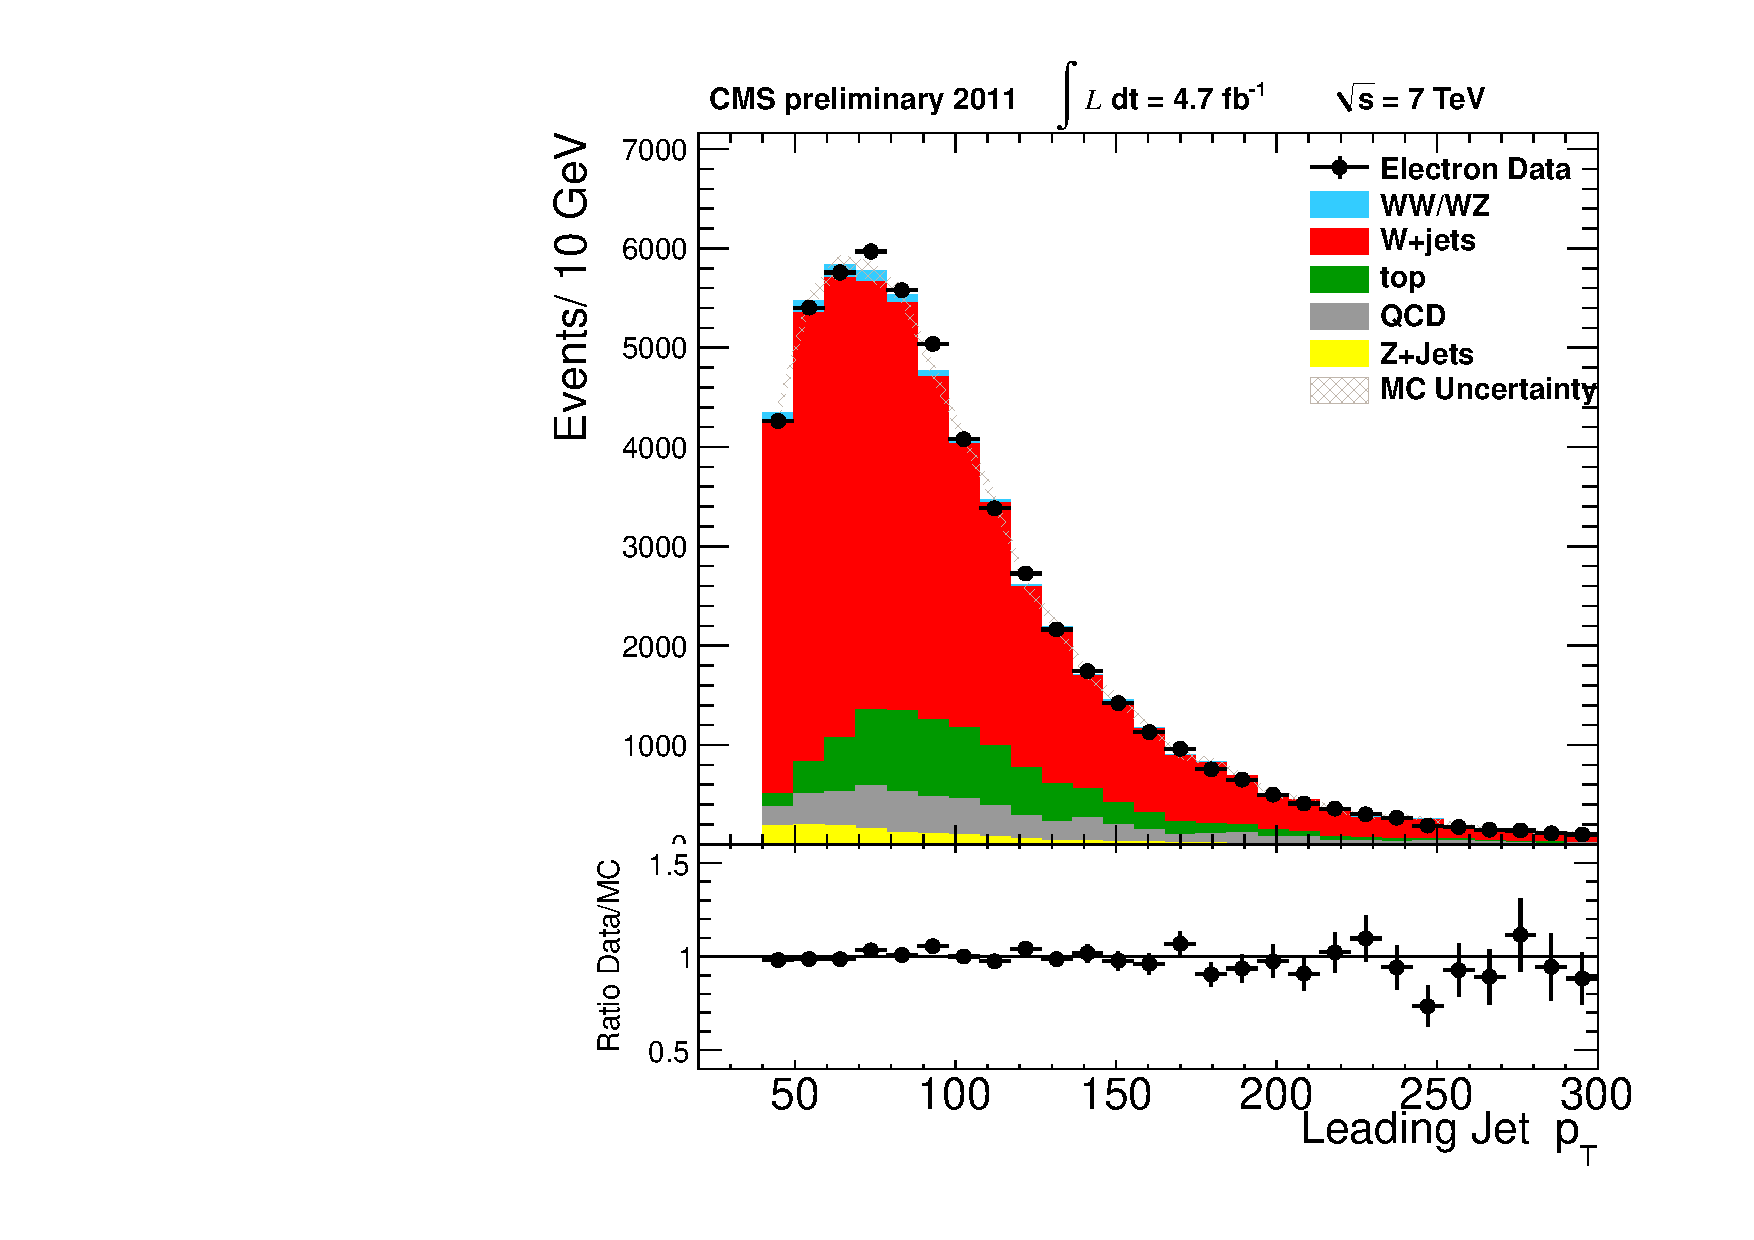
\includegraphics[width=0.49\textwidth]{figs/n-1_plots_el/el_jetld_pt.pdf}
    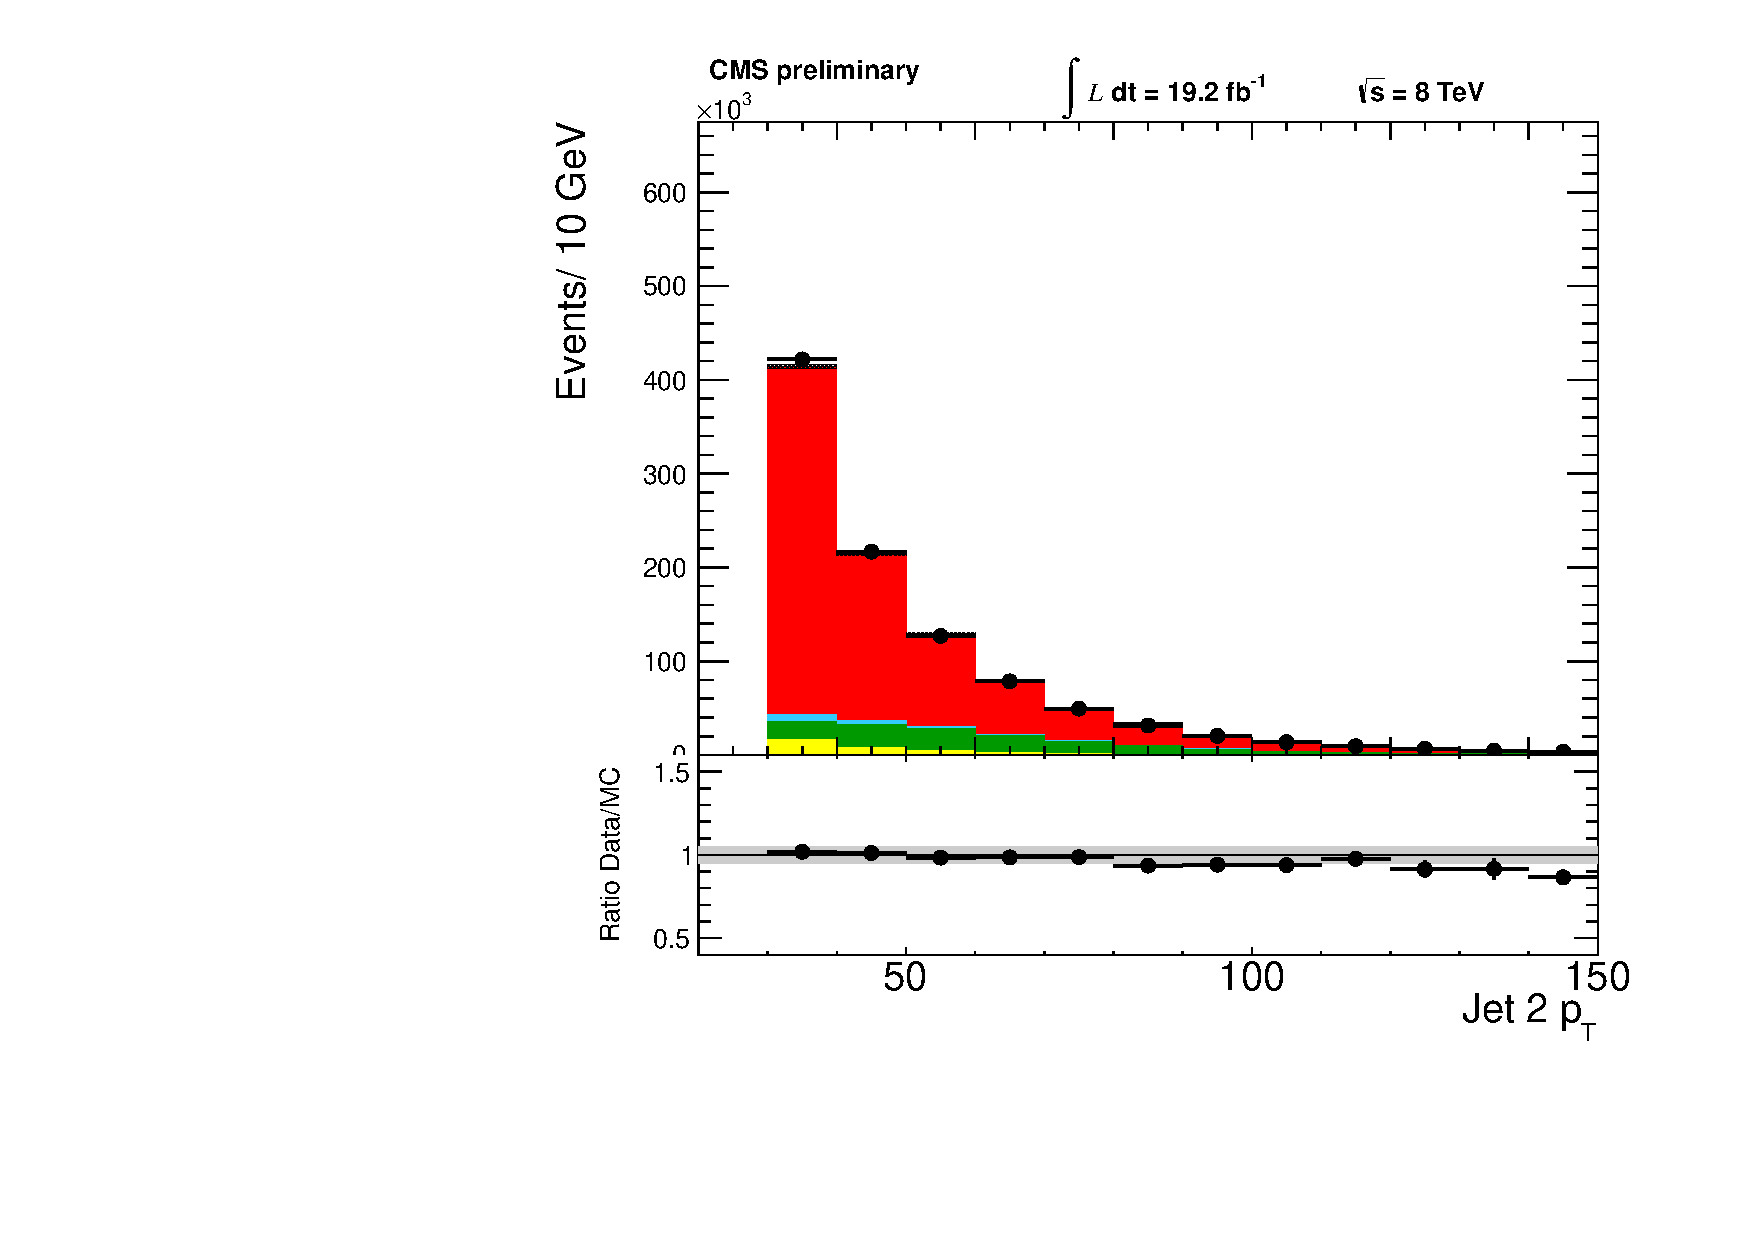
\includegraphics[width=0.49\textwidth]{figs/n-1_plots_el/el_jetnt_pt.pdf}
    \caption{Comparison of the leading jet $p_{T} $ (left) and the
      second leading jet $p_{T} $ (right) distributions from data and MC
      for the electron+jets selection. 
      }
    \label{fig:elec_jet_pt}}
\end{figure}
%%%%%%%%%%%%%%%%%%%%%%%%%%%%
\begin{figure}[h!t]
  {\centering
    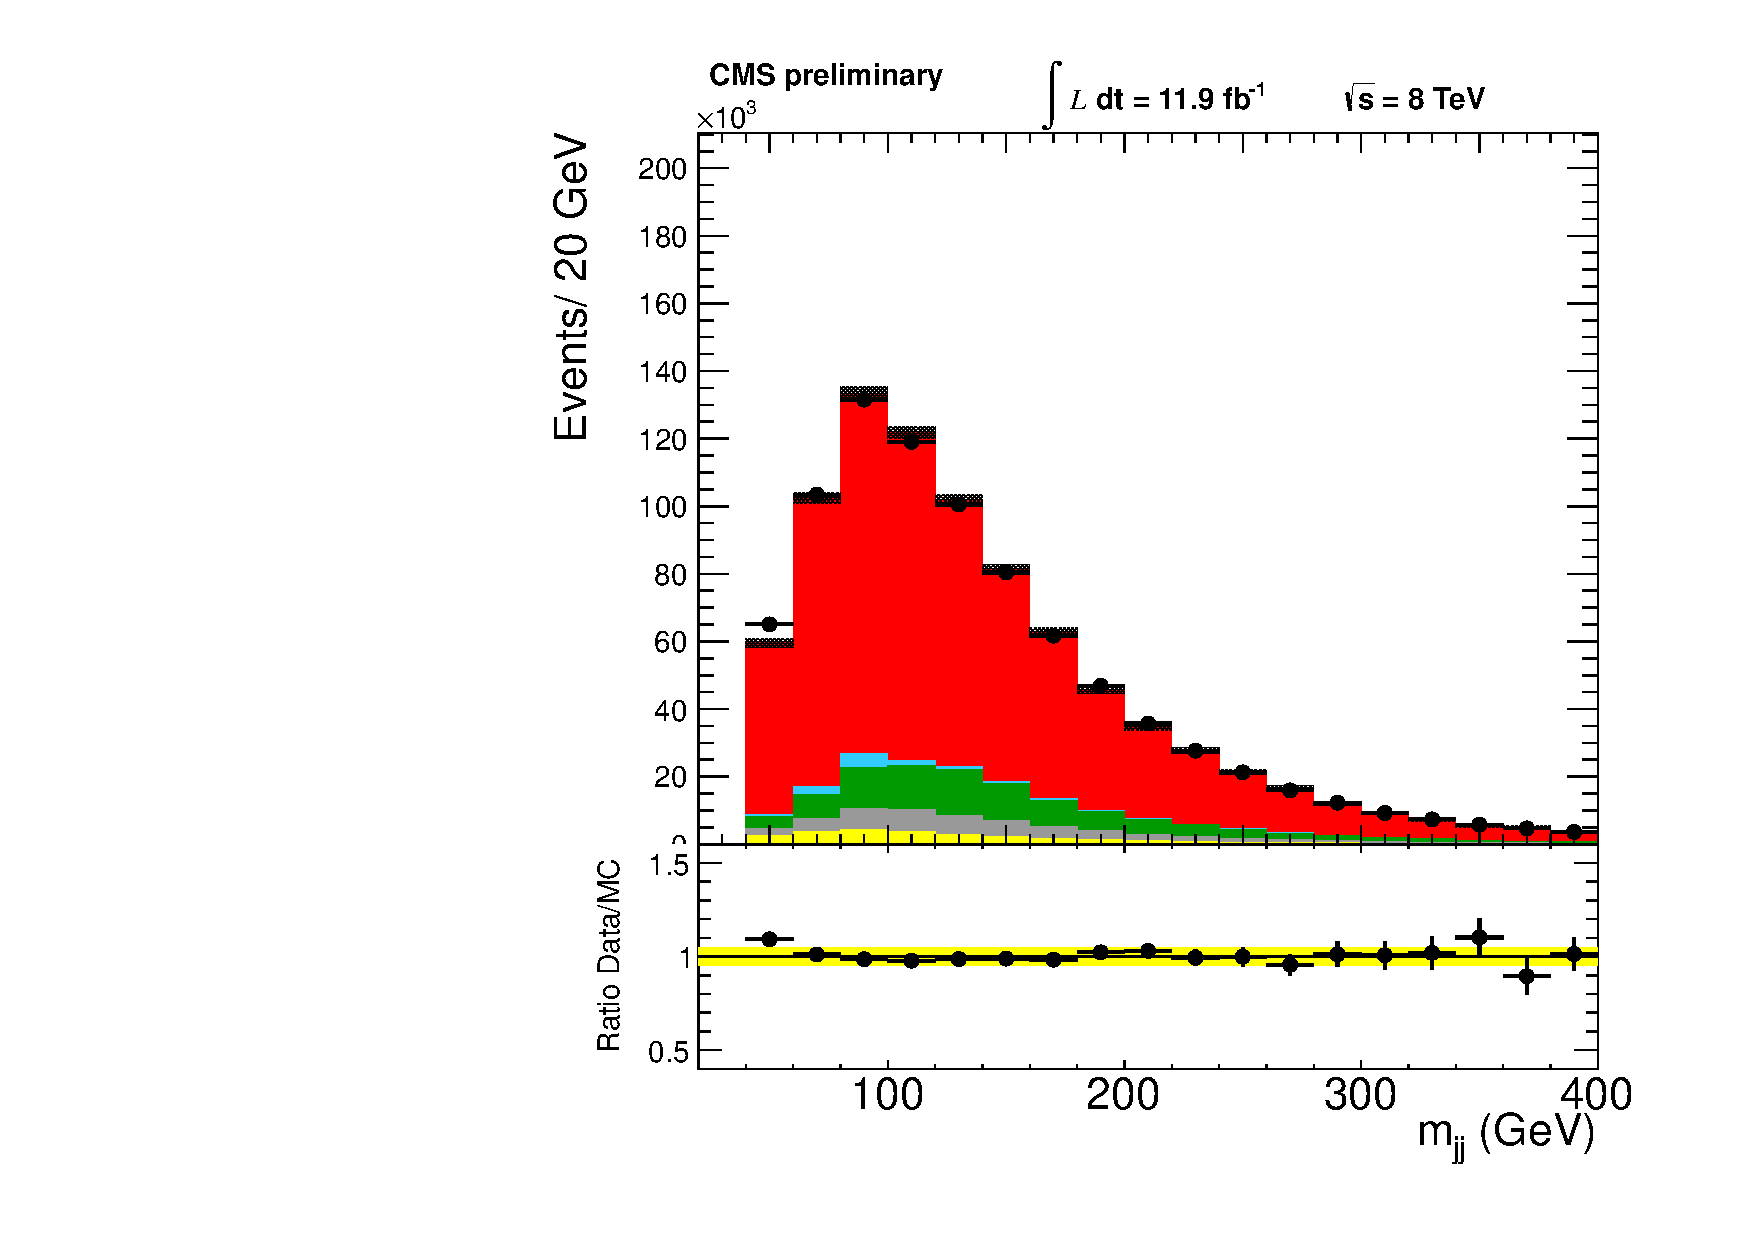
\includegraphics[width=0.49\textwidth]{figs/n-1_plots_el/el_mjj.pdf}
    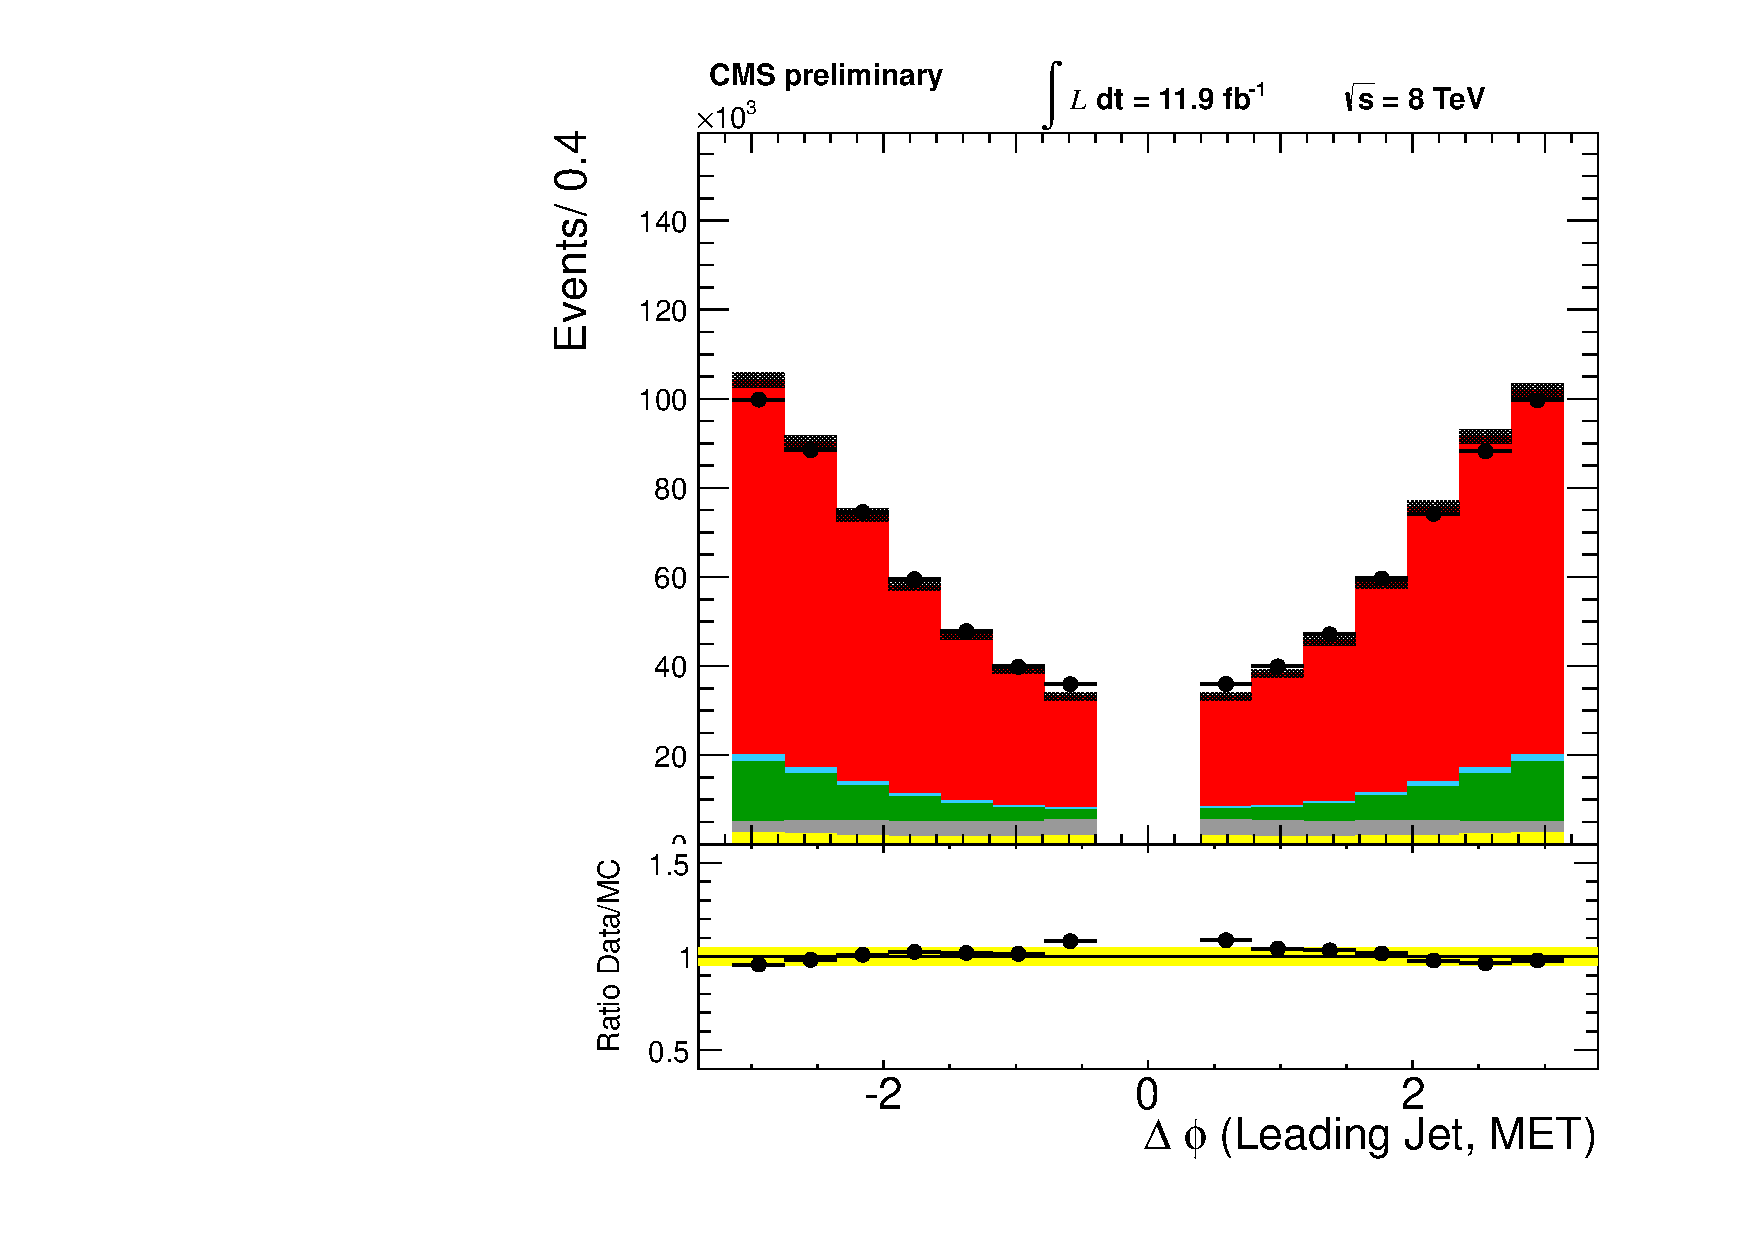
\includegraphics[width=0.49\textwidth]{figs/n-1_plots_el/el_deltaphi_jetldmet.pdf}

    \caption{Comparison of the distributions from data and MC of the
    dijet mass (left) and the $\Delta \phi $ between the leading jet and MET (right)
    for the electron+jets selection.}
    \label{fig:elec_dijetmass}}
\end{figure}
\begin{figure}[h!t]
  {\centering
    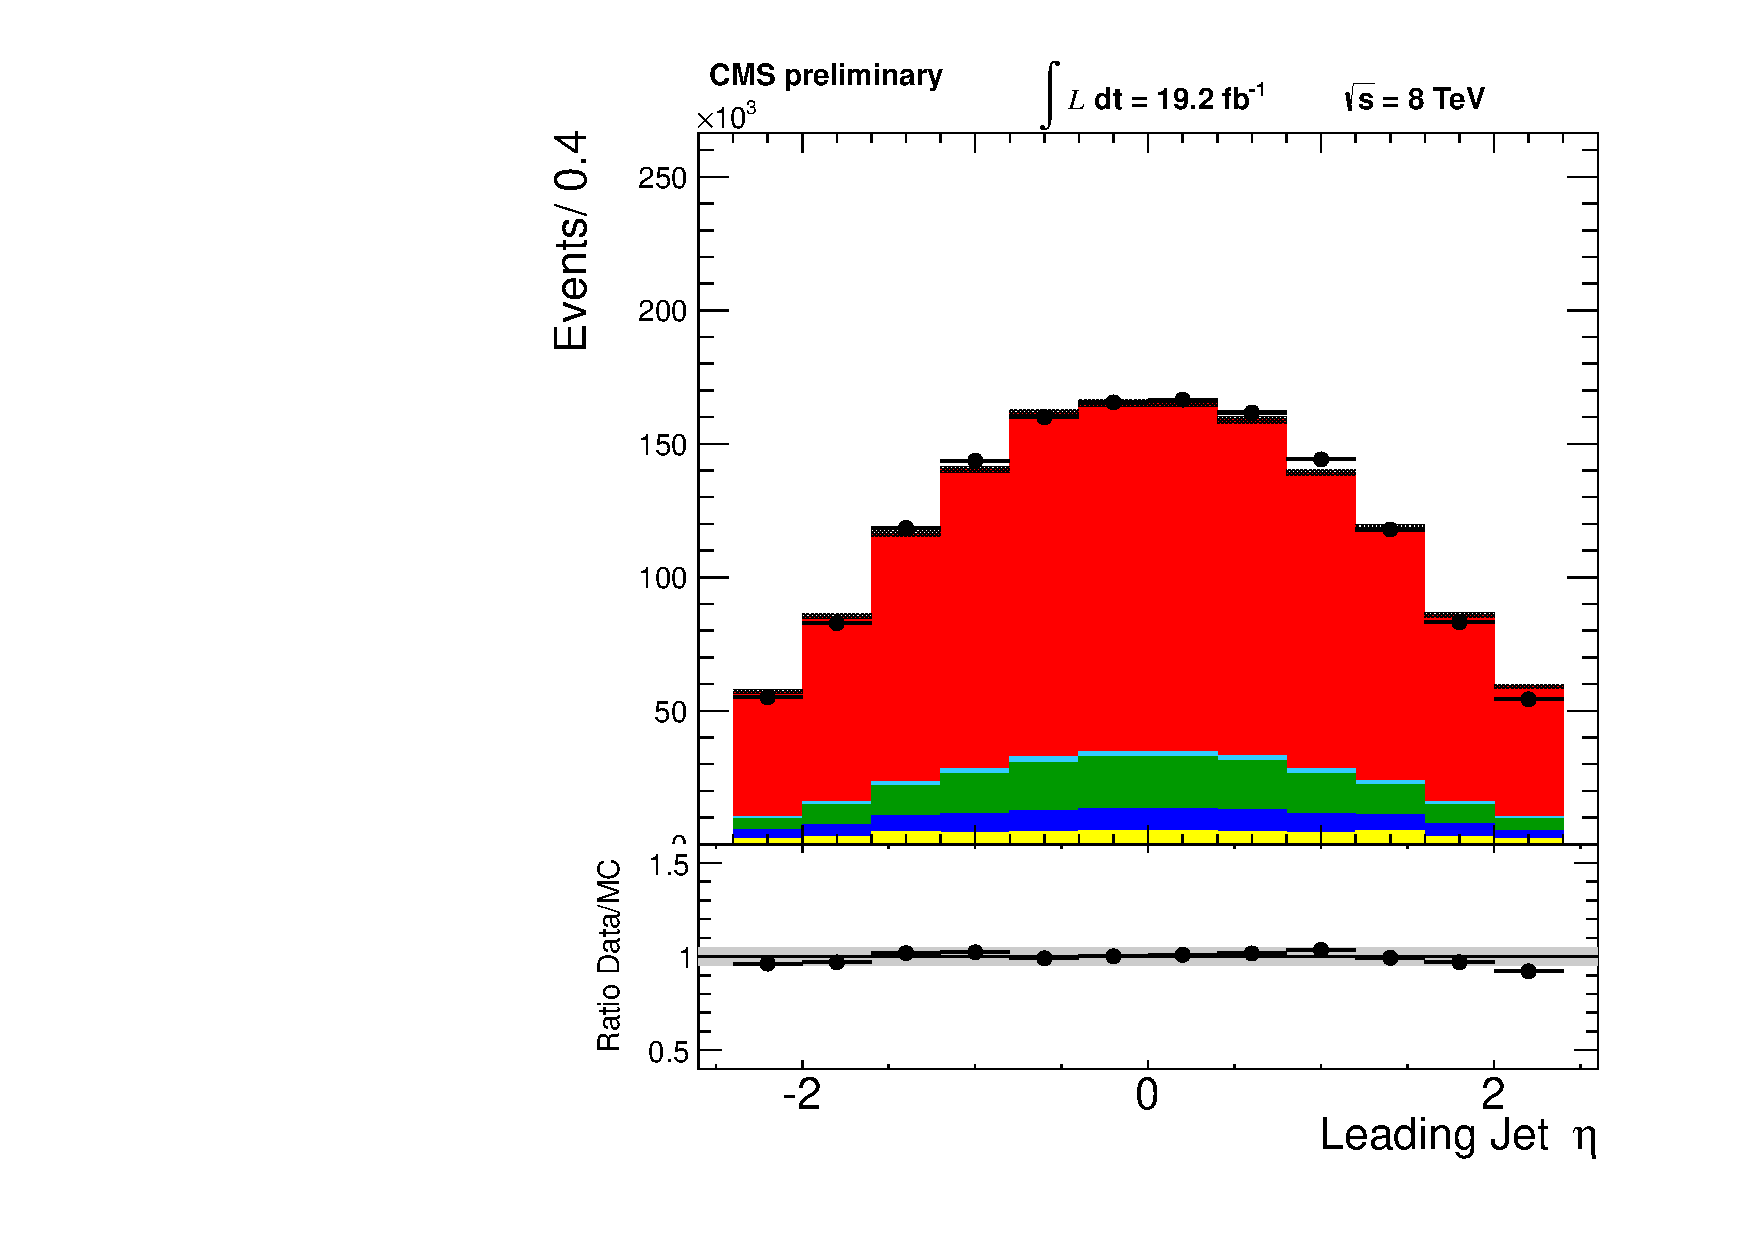
\includegraphics[width=0.49\textwidth]{figs/n-1_plots_el/el_jetld_eta.pdf}
    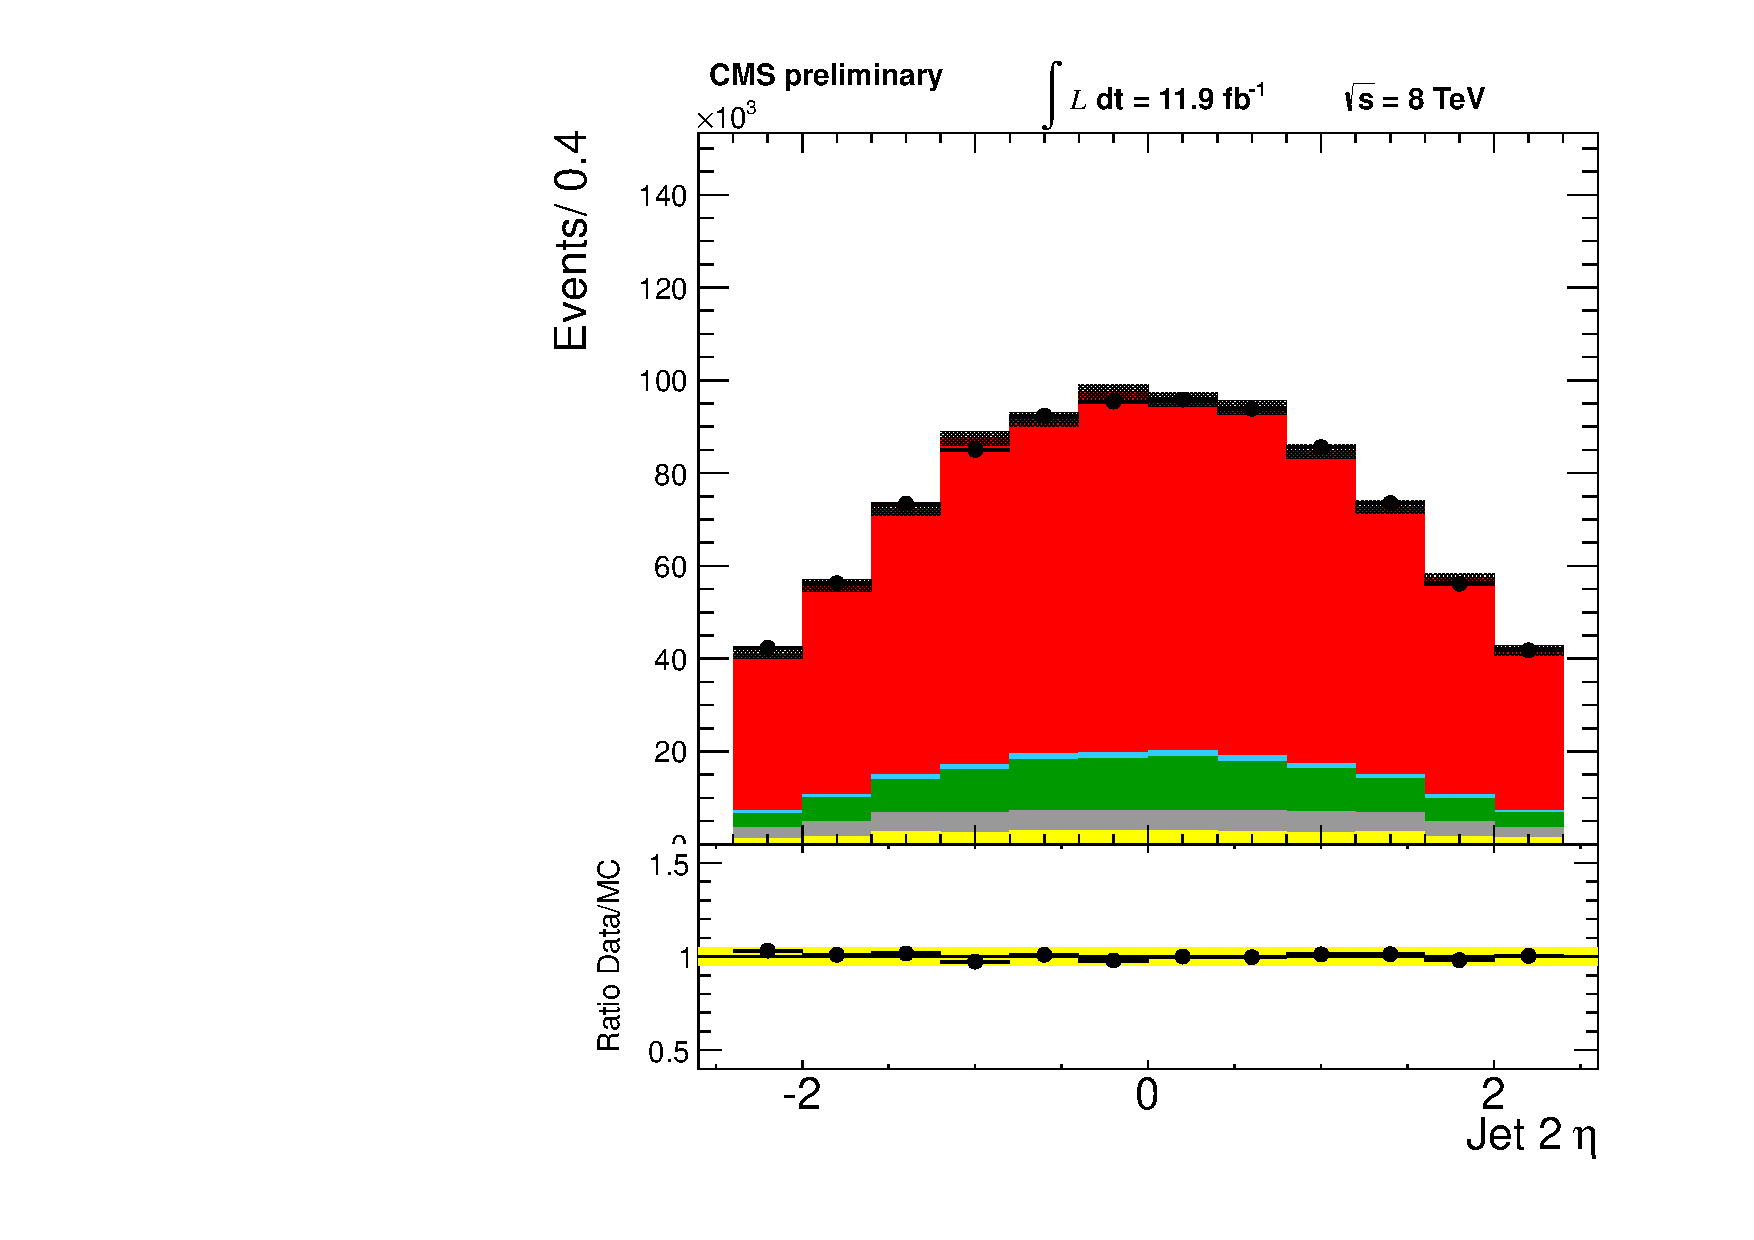
\includegraphics[width=0.49\textwidth]{figs/n-1_plots_el/el_jetnt_eta.pdf}
    \caption{Comparison of the leading jet $\eta $ (left) and the
      second leading jet $\eta $ (right) distributions from data and MC for the electron+jets
      selection. 
      }
    \label{fig:elec_jet_eta}}
\end{figure}
%%%%%%%%%%%%%%%%%%%%%%%%%%%%
\begin{figure}[h!t]
  {\centering
    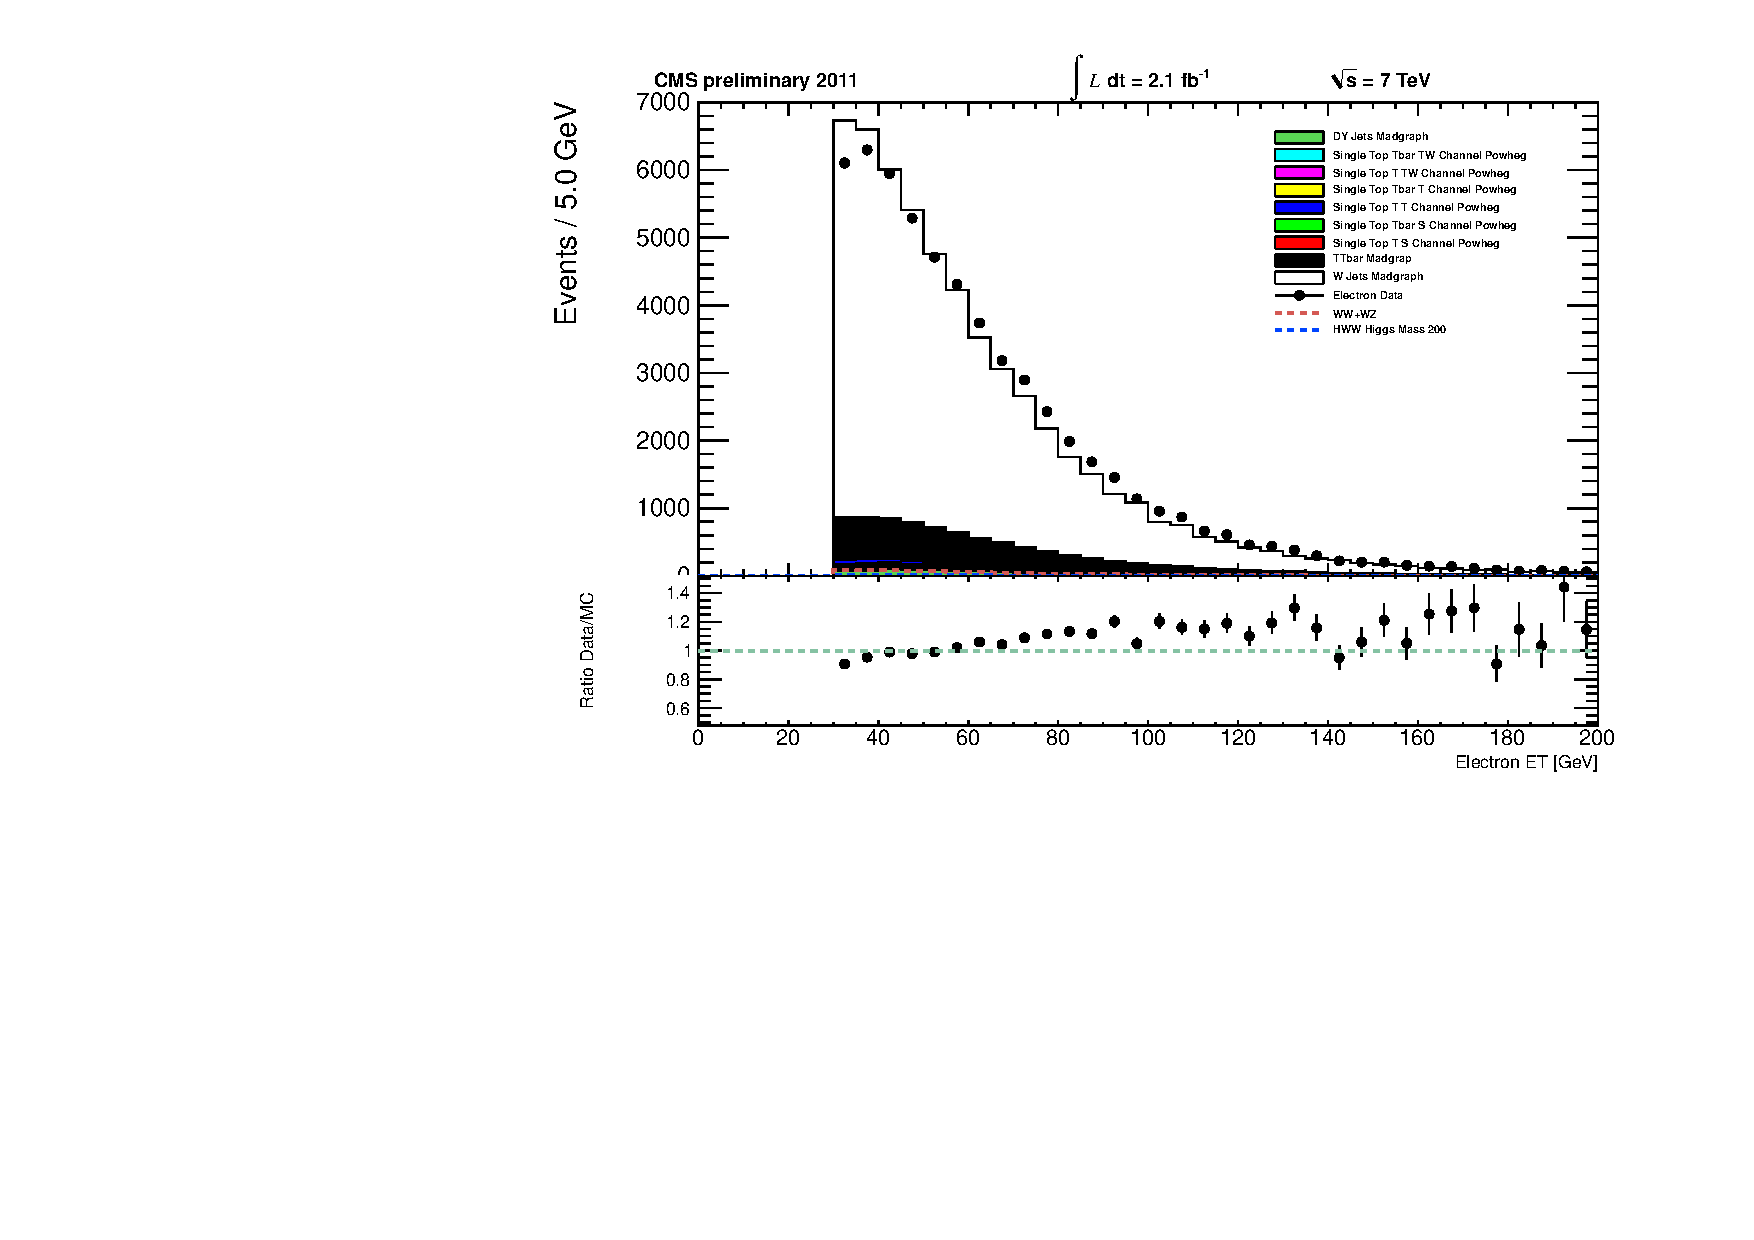
\includegraphics[width=0.49\textwidth]{figs/n-1_plots_el/el_W_electron_et.pdf}
    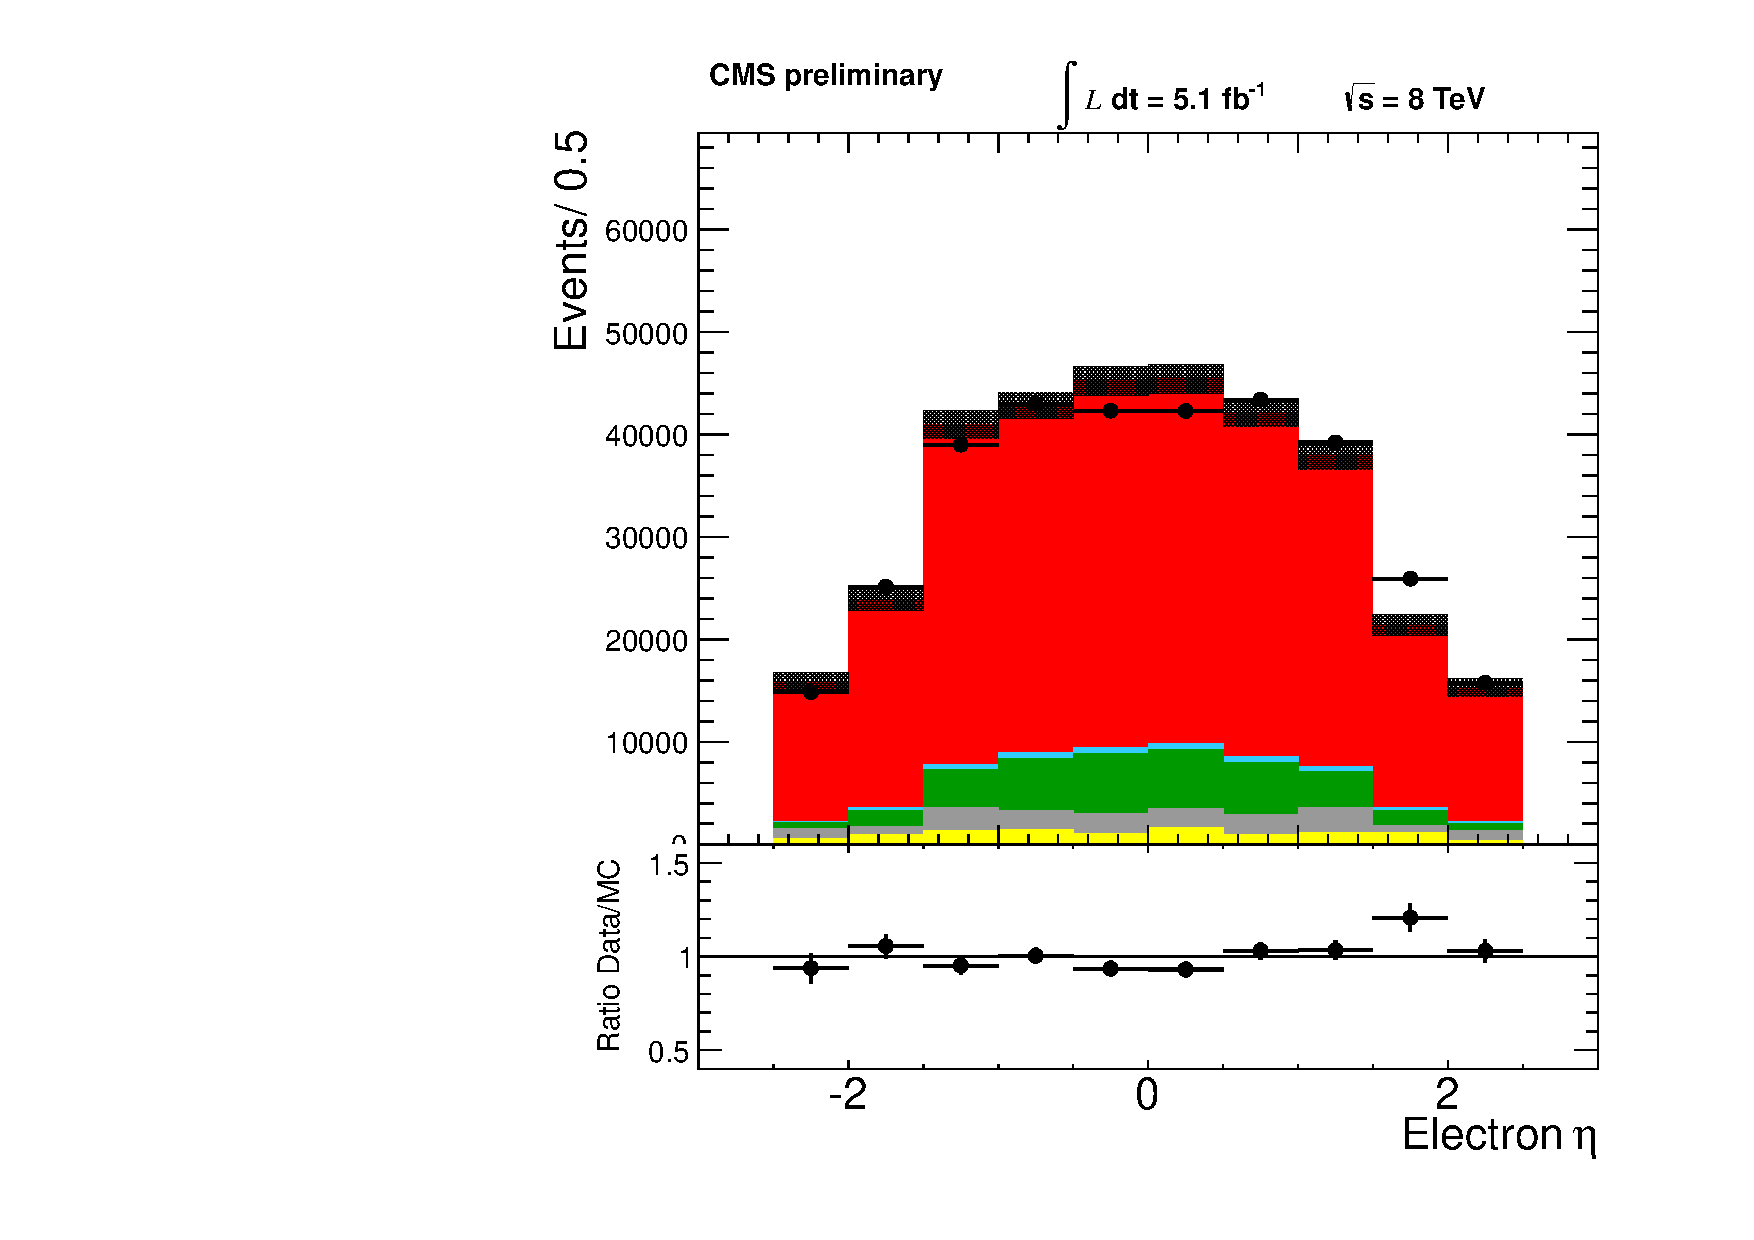
\includegraphics[width=0.49\textwidth]{figs/n-1_plots_el/el_W_electron_eta.pdf}
    \caption{Comparison of the electron $E_{T} $ (left) and the
    electron $\eta $ (right) distributions from data and MC for the
    electron+jets selection. 
    }
   \label{fig:elec_electron}}
\end{figure}
%%%%%%%%%%%%%%%%%%%%%%%%%%%%
\begin{figure}[h!t]
  {\centering
    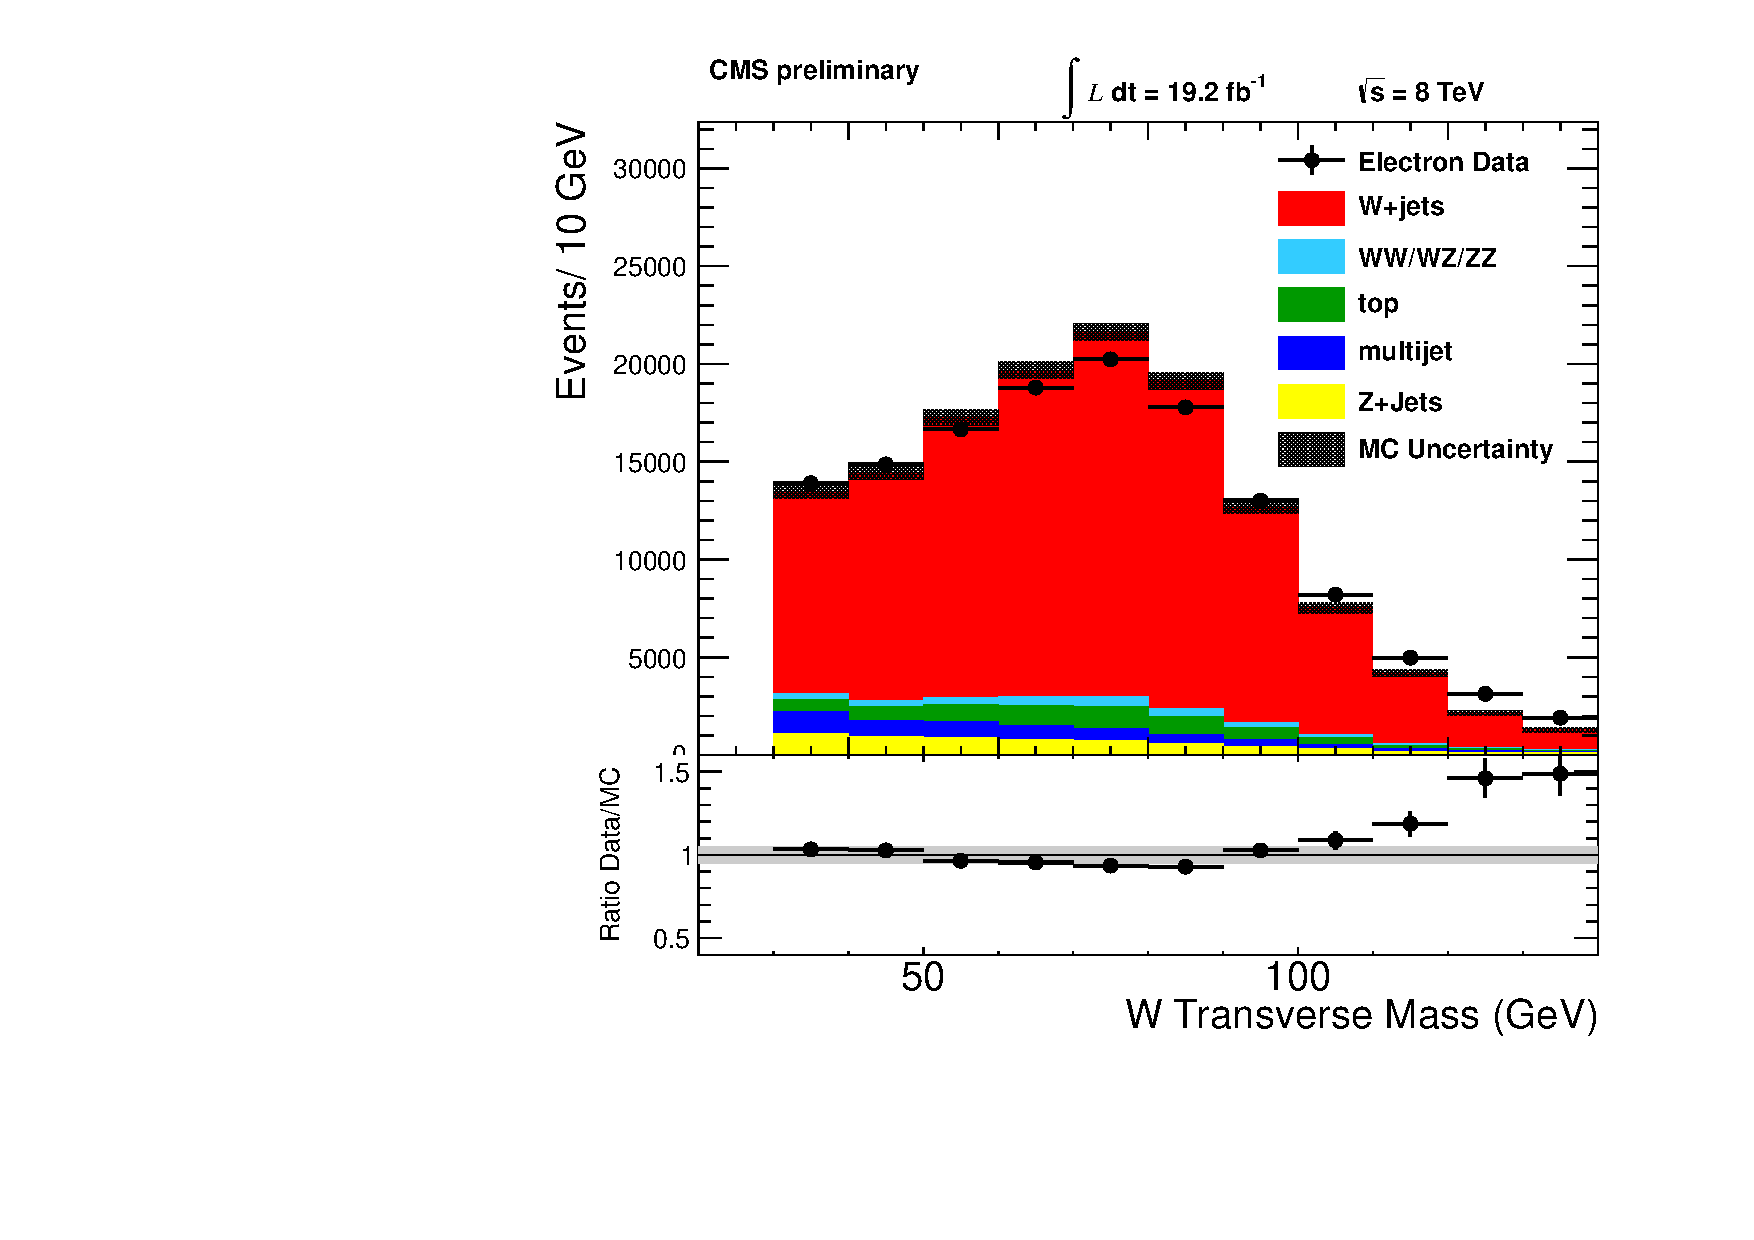
\includegraphics[width=0.49\textwidth]{figs/n-1_plots_el/el_W_mt.pdf}
    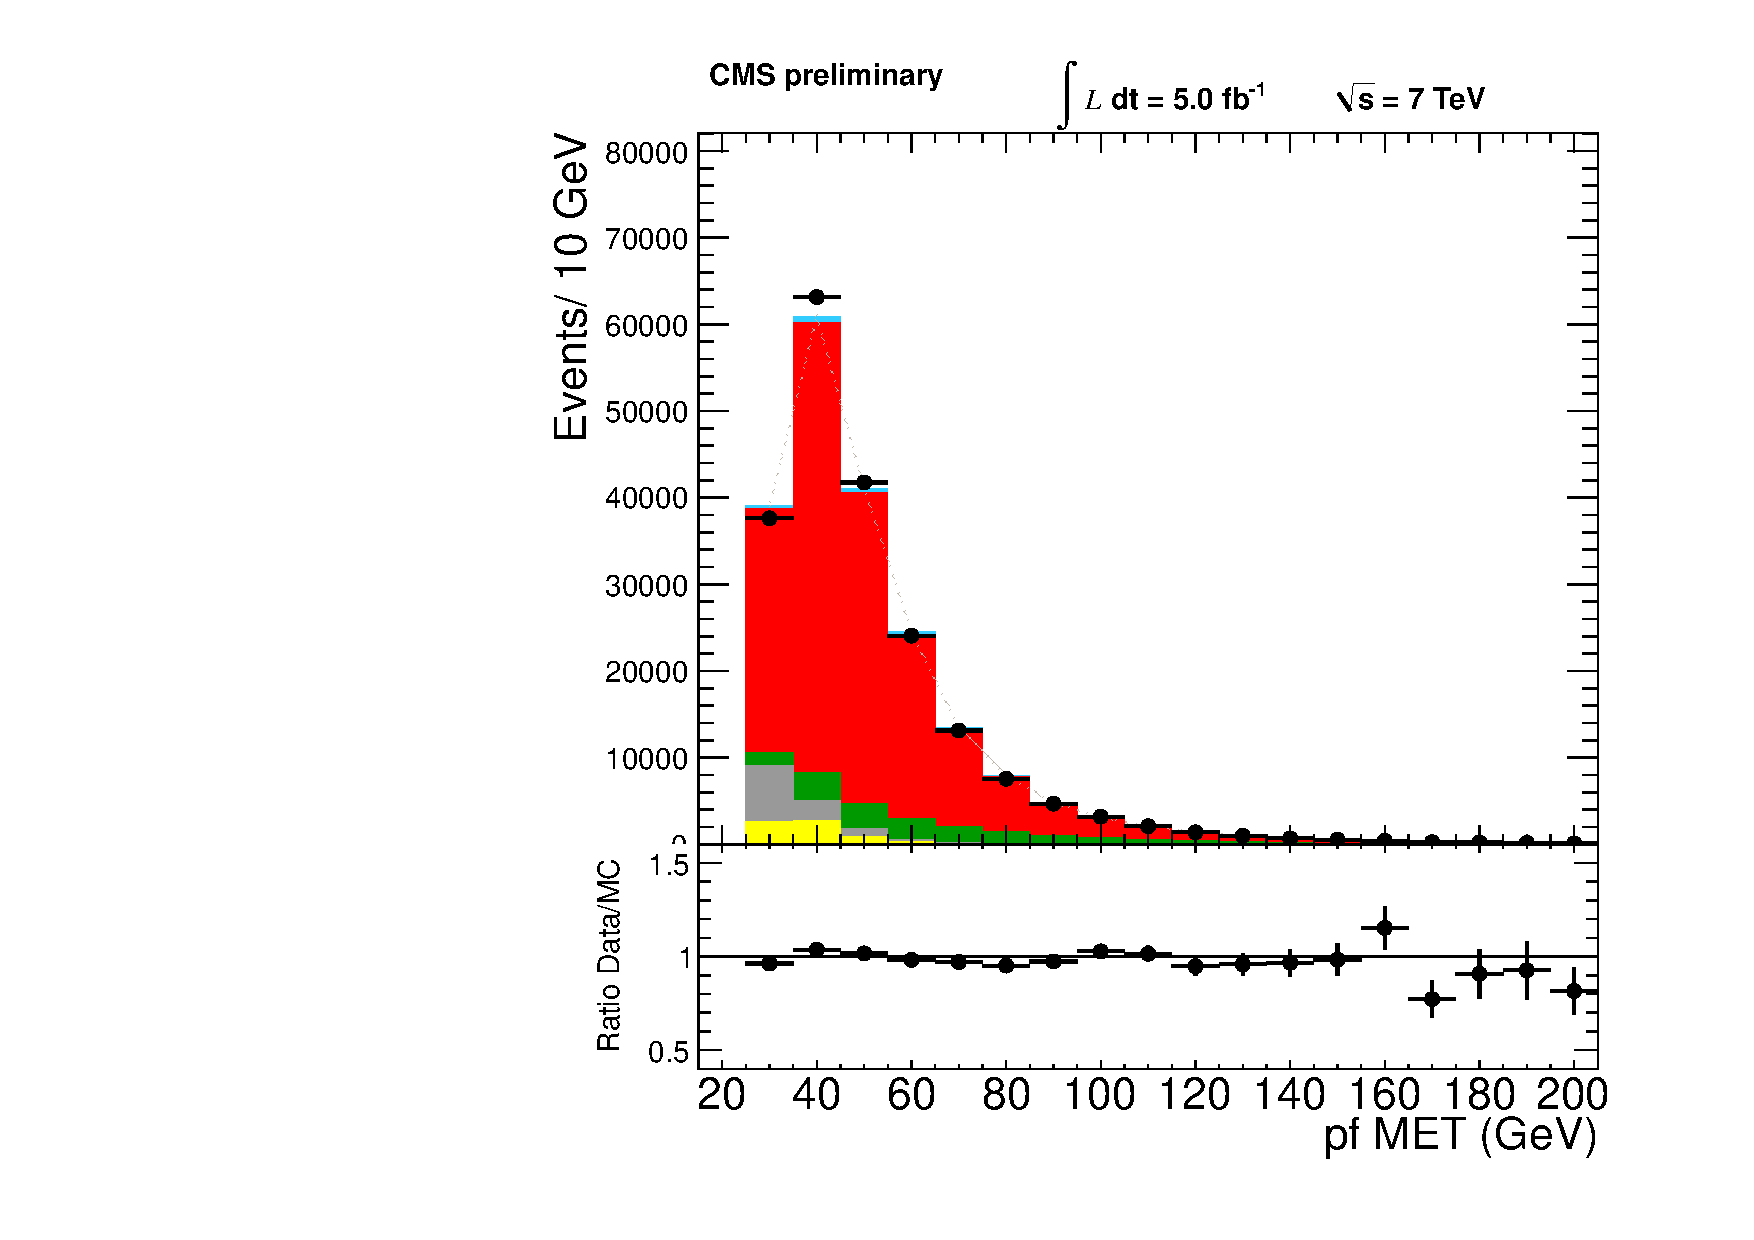
\includegraphics[width=0.49\textwidth]{figs/n-1_plots_el/el_event_met_pfmet.pdf}
    \caption{Comparison of the distributions from data and MC of the transverse mass
     of electron / MET system (left) and the MET (right) for the
      electron+jets selection. 
      }
    \label{fig:elec_W_Mt}}
\end{figure}
%%%%%%%%%%%%%%%%%%%%%%%%%%%%
\begin{figure}[h!t]
  {\centering
    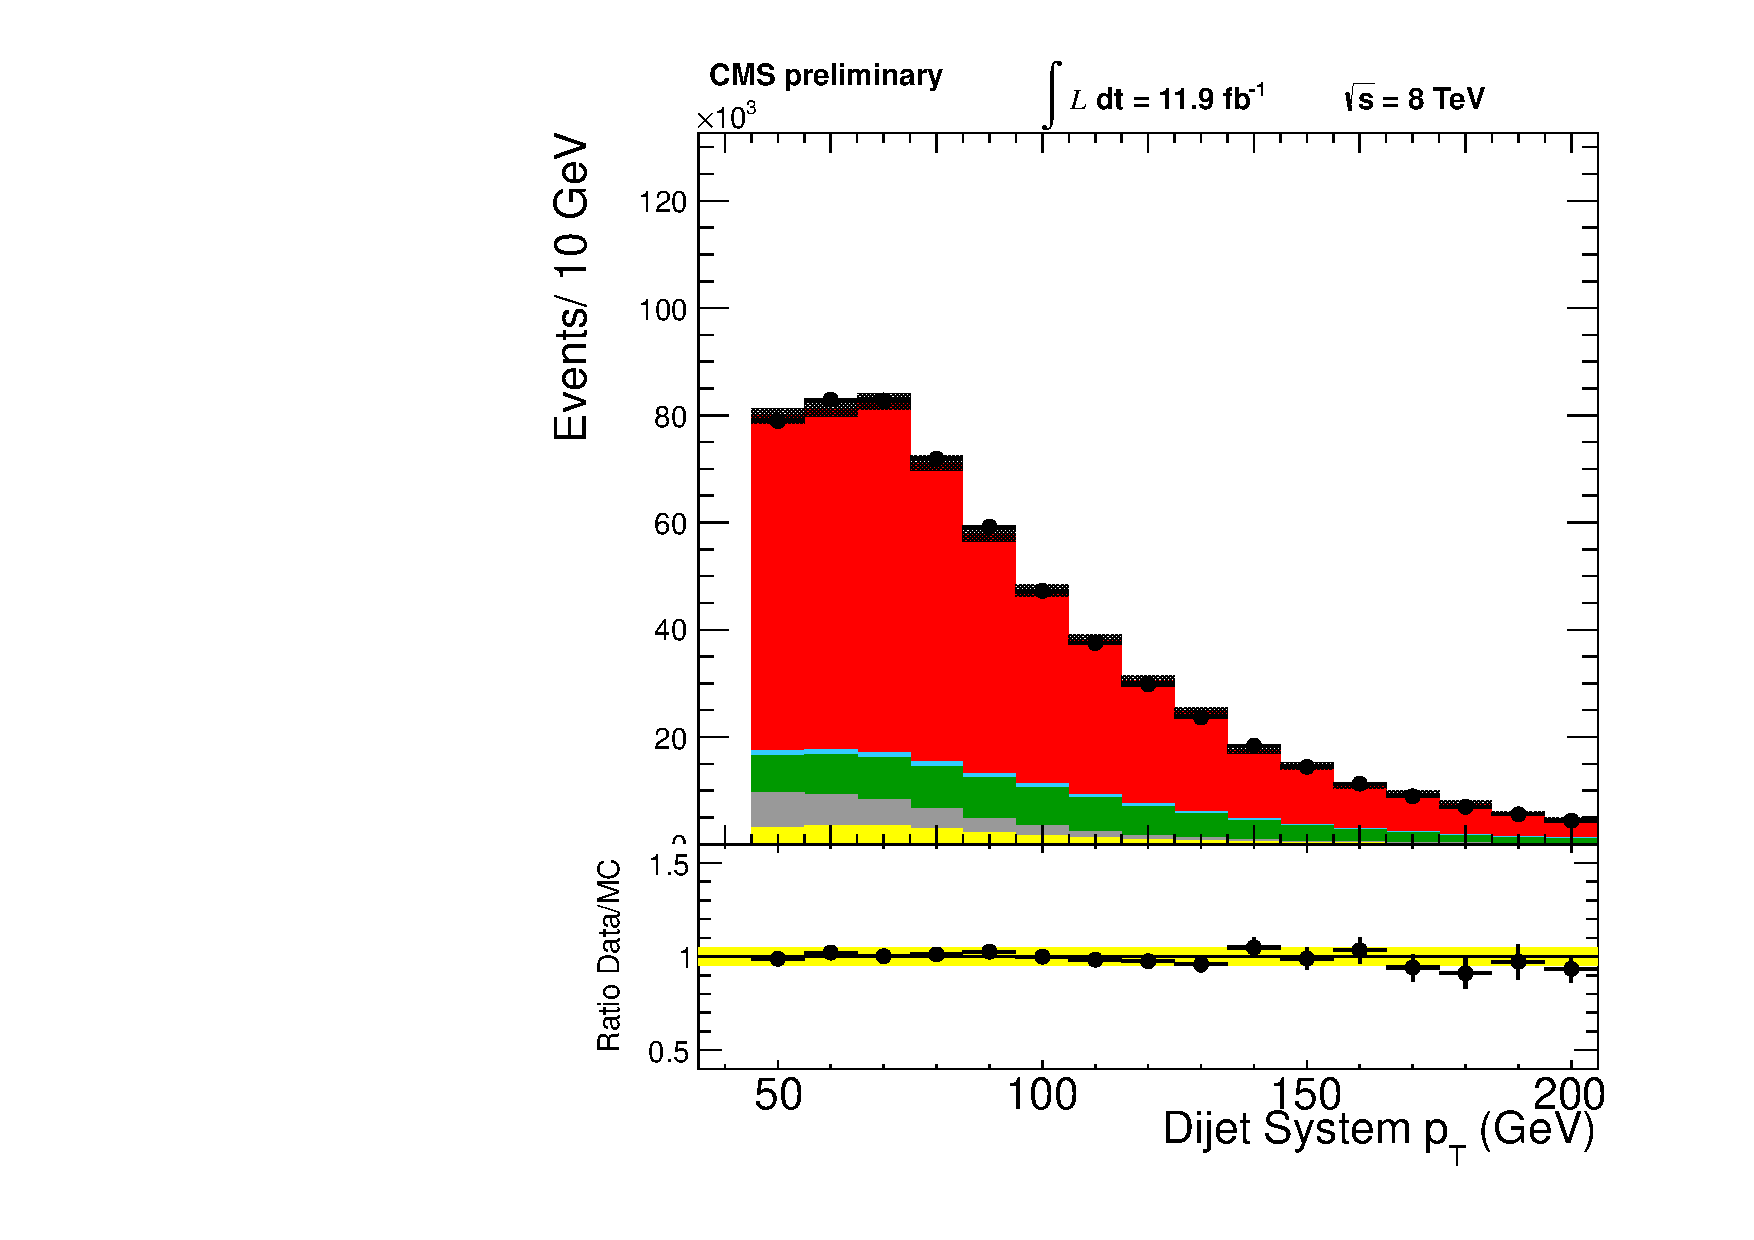
\includegraphics[width=0.49\textwidth]{figs/n-1_plots_el/el_dijet_pt.pdf}
    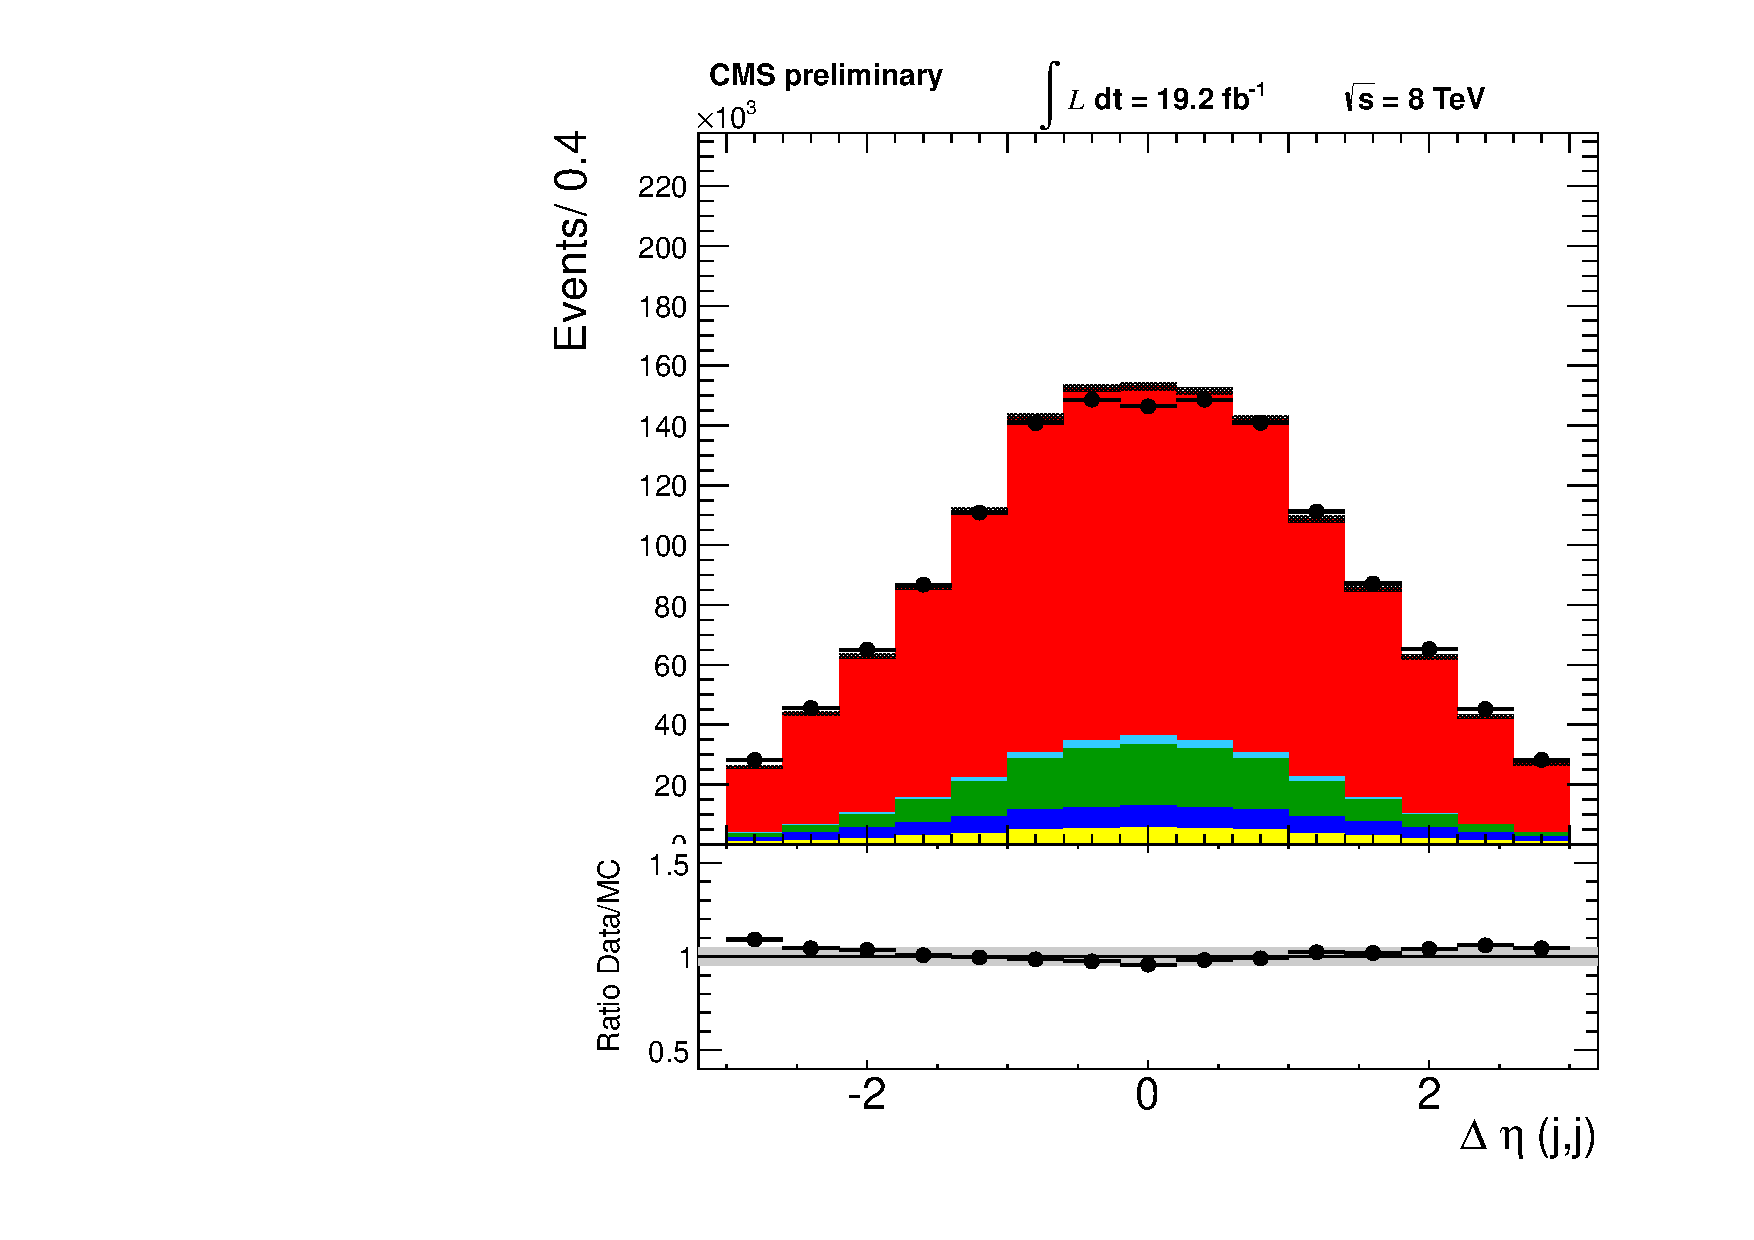
\includegraphics[width=0.49\textwidth]{figs/n-1_plots_el/el_deltaeta_jj.pdf}
    \caption{Comparison of the distributions from data and MC of the dijet system
     $p_{T}$ (left) and the $\eta $ separation between the two jets (right) for the
      electron+jets selection. 
      }
    \label{fig:elec_dijet}}
\end{figure}
%%%%%%%%%%%%%%%%%%%%%%%%%%%%
%%%%%%%%%%%%%%%%%%%%%%%%%%%%
\begin{figure}[htbp]
\centering
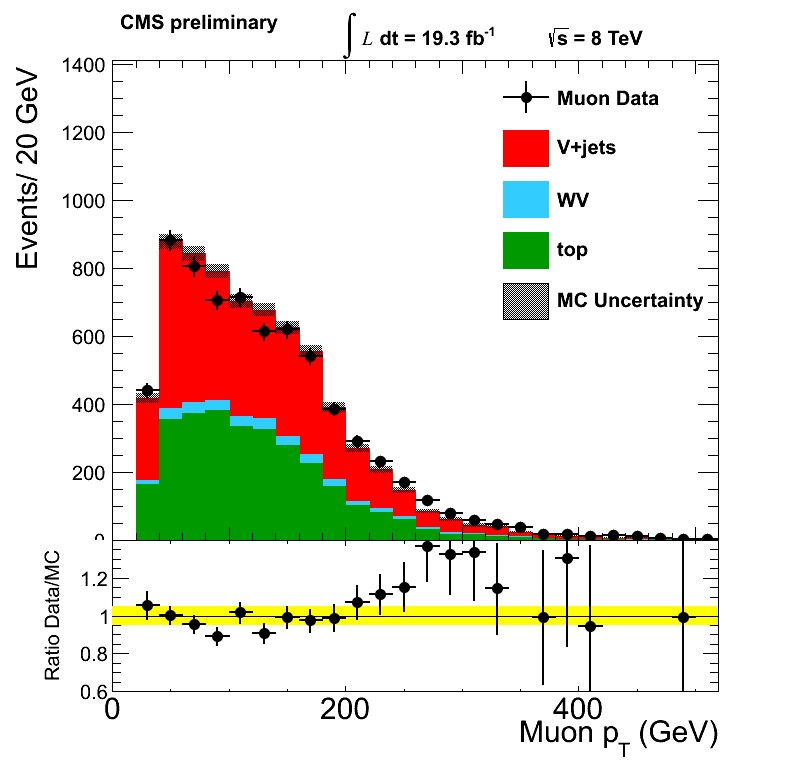
\includegraphics[width=0.45\textwidth]{figs/n-1_plots_mu/mu_W_muon_pt.png}
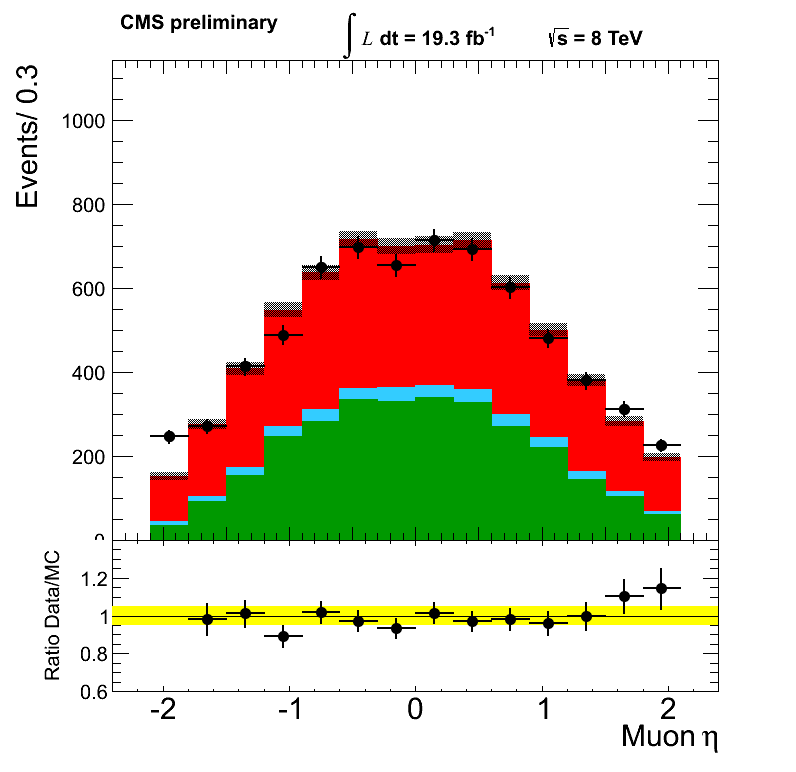
\includegraphics[width=0.45\textwidth]{figs/n-1_plots_mu/mu_W_muon_eta.png}
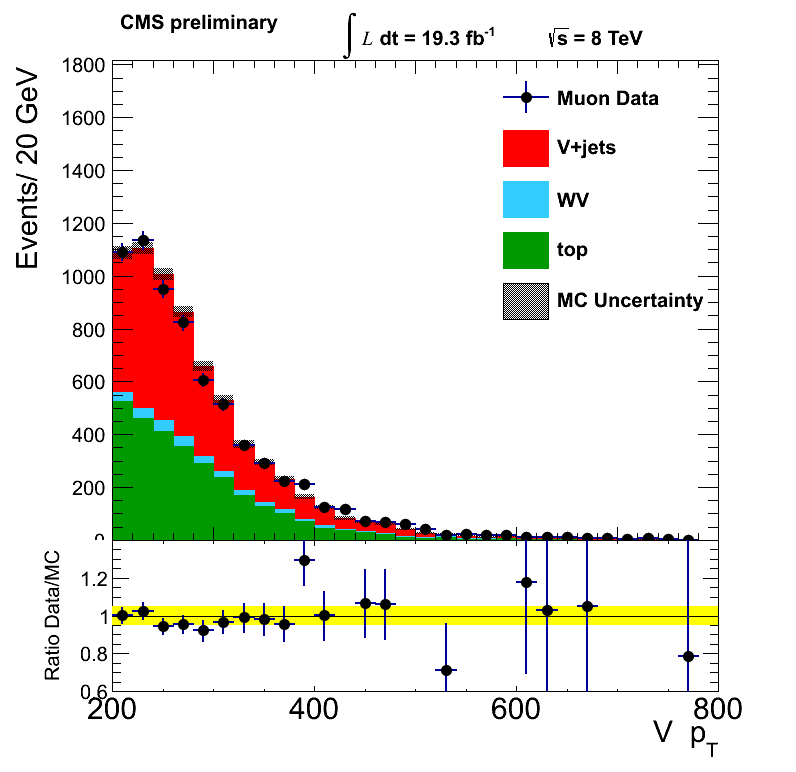
\includegraphics[width=0.45\textwidth]{figs/n-1_plots_mu/mu_W_pt.png}
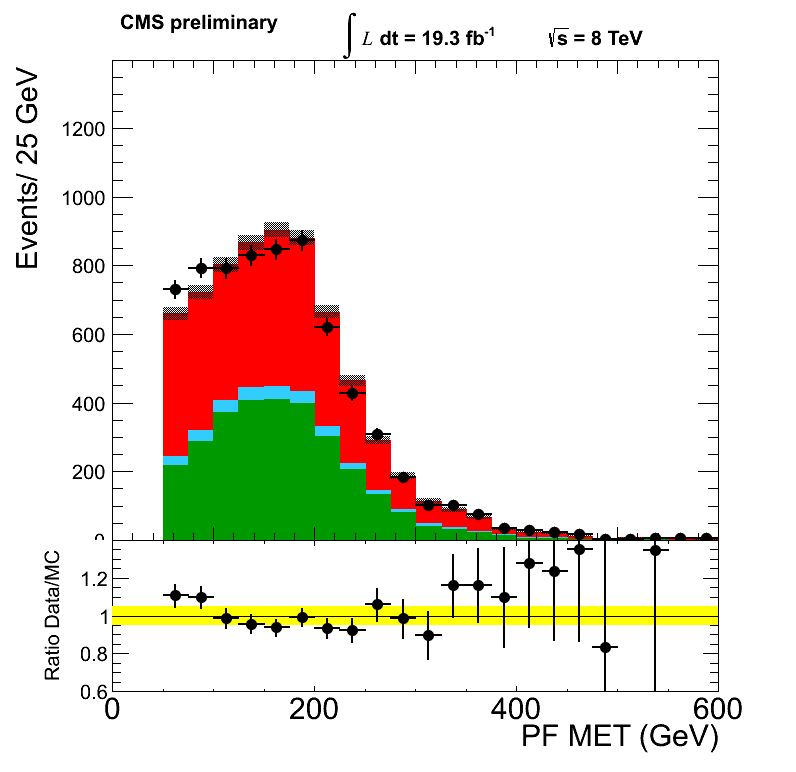
\includegraphics[width=0.45\textwidth]{figs/n-1_plots_mu/mu_event_met_pfmet.png}\\
\caption{Boosted configuration control plots for muon channel: muon pT and $\eta$, W pT and MVA MET.}
\label{fig:control_boosted_mu}
\end{figure}

\begin{figure}[htbp]
\centering
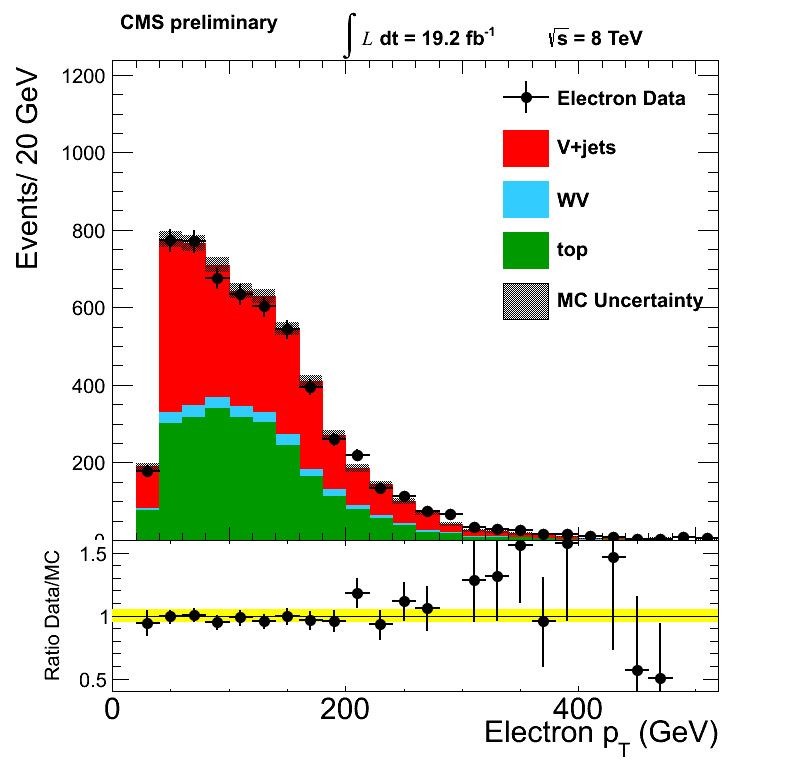
\includegraphics[width=0.45\textwidth]{figs/n-1_plots_el/el_W_elec_pt.png}
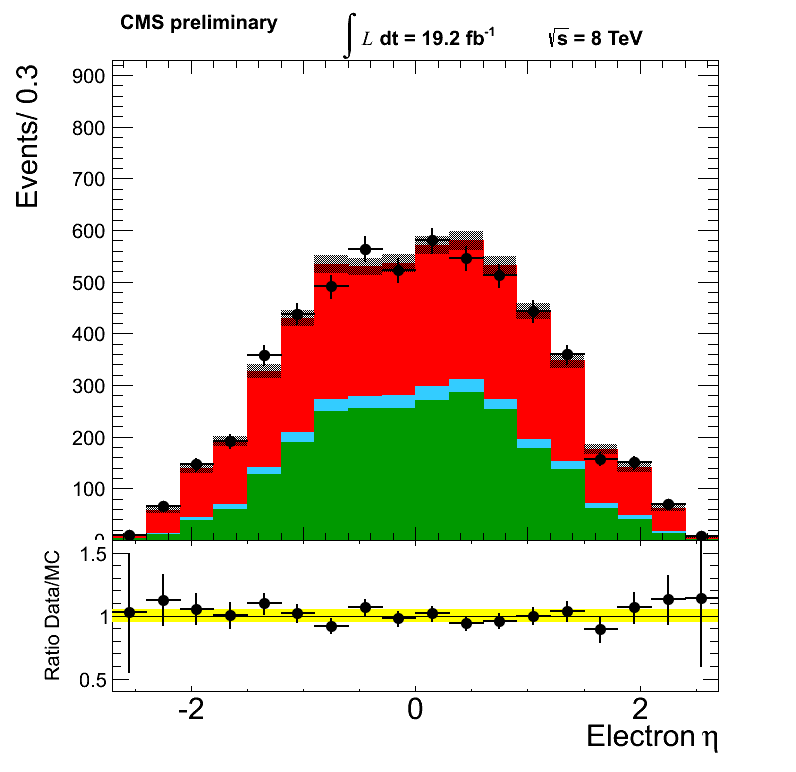
\includegraphics[width=0.45\textwidth]{figs/n-1_plots_el/el_W_elec_eta.png}\\
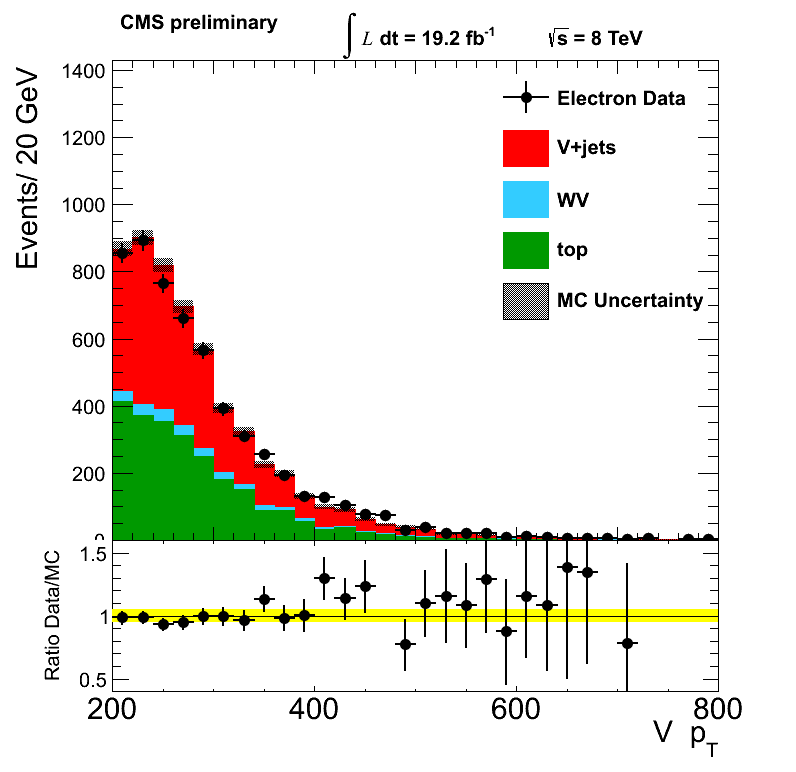
\includegraphics[width=0.45\textwidth]{figs/n-1_plots_el/el_W_pt.png}
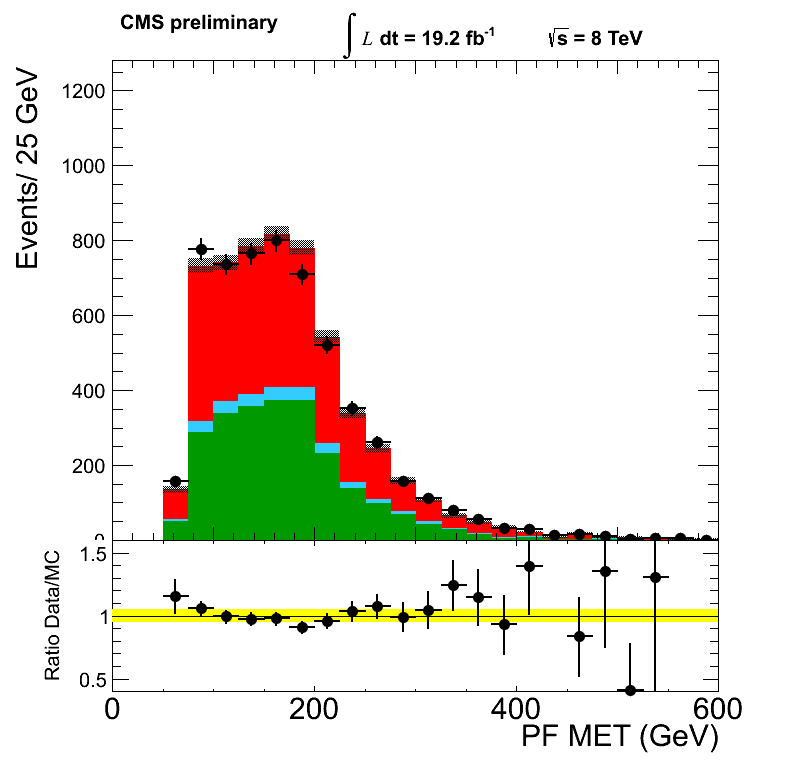
\includegraphics[width=0.45\textwidth]{figs/n-1_plots_el/el_event_met_pfmet.png}
\caption{Boosted configuration control plots for electron channel: electron pT and $\eta$, W pT and MVA MET.}
\label{fig:control_boosted_el}
\end{figure}

\begin{figure}[htbp]
\centering
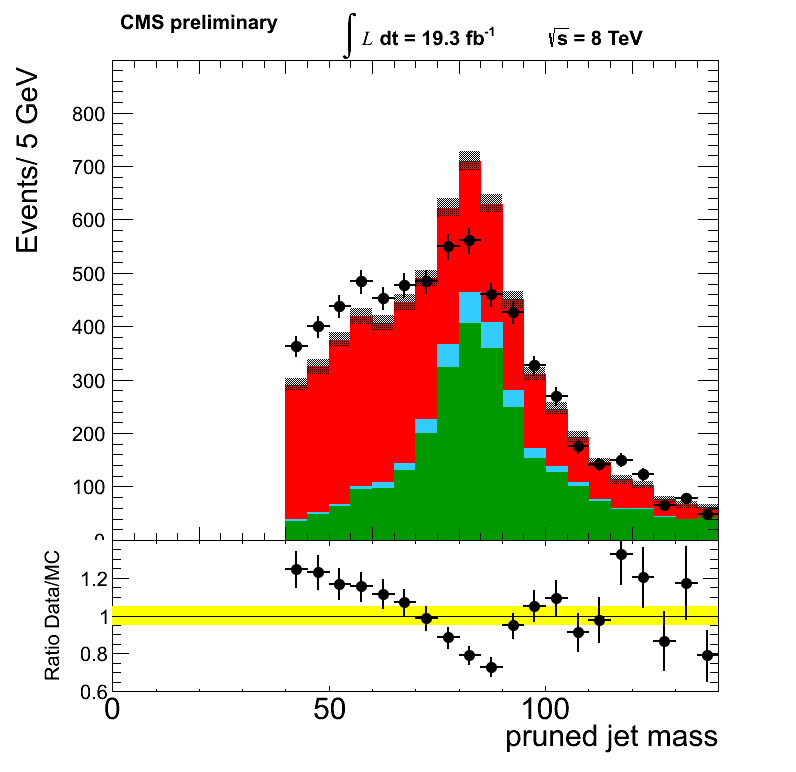
\includegraphics[width=0.45\textwidth]{figs/n-1_plots_mu/mu_GroomedJet_mass.png}
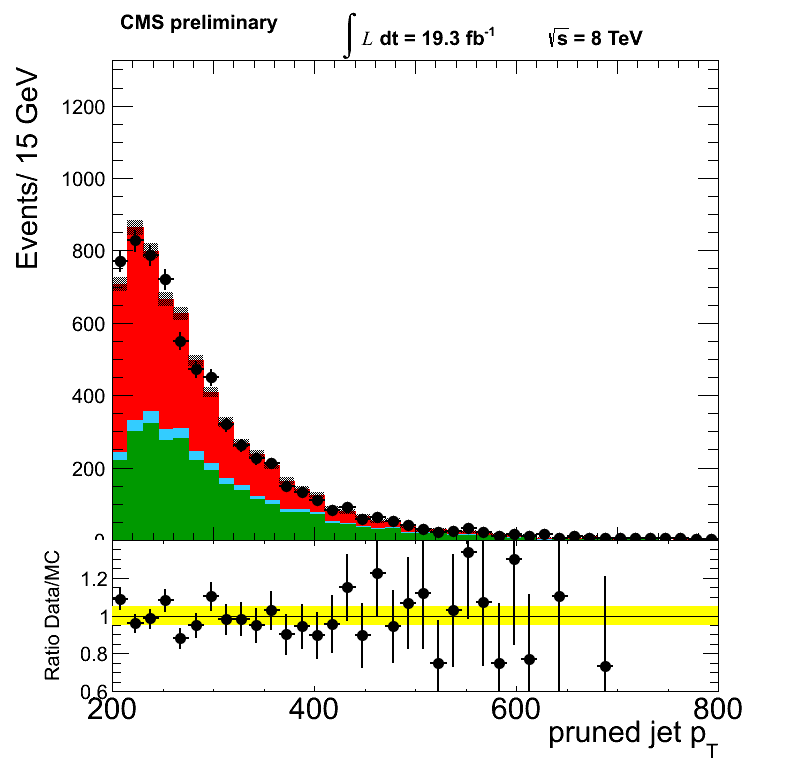
\includegraphics[width=0.45\textwidth]{figs/n-1_plots_mu/mu_GroomedJet_pt_pr.png}\\
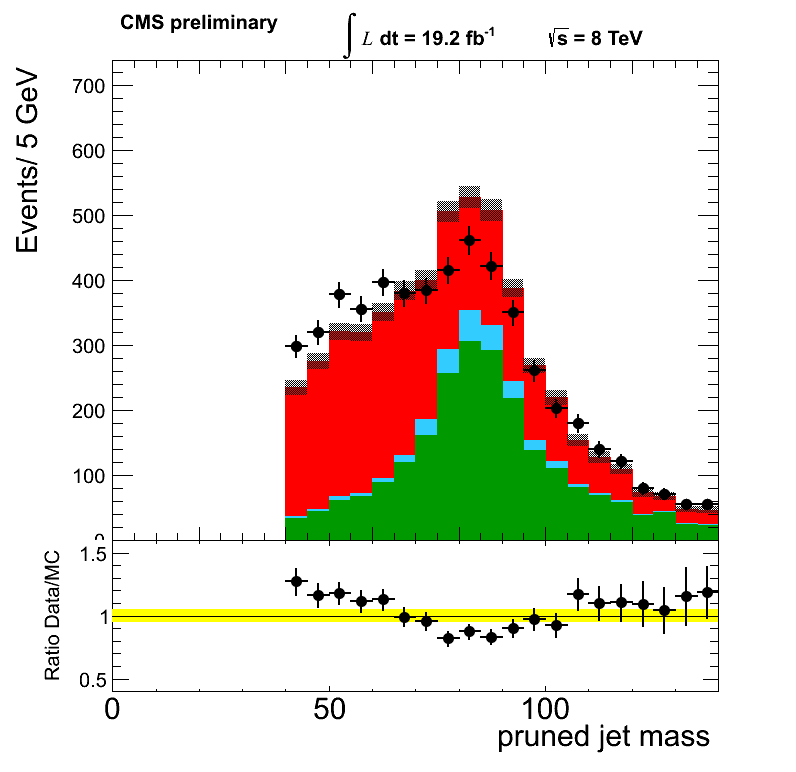
\includegraphics[width=0.45\textwidth]{figs/n-1_plots_el/el_GroomedJet_mass.png}
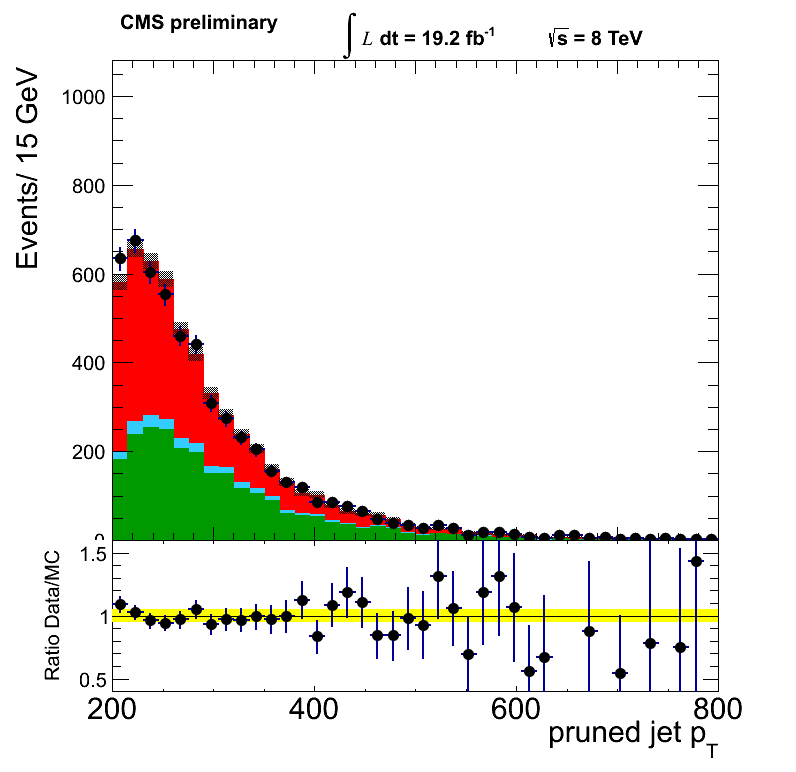
\includegraphics[width=0.45\textwidth]{figs/n-1_plots_el/el_GroomedJet_pt_pr.png}\\
\caption{Boosted configuration control plots: pruned jet mass and pruned jet pT for muon (top) and electron (bottom) channels.}
\label{fig:control_boosted_jet}
\end{figure}
%%%%%%%%%%%%%%%%%%%%%%%%%%%%
%%%%%%%%%%%%%%%%%%%%%%%%%%%%
%%%%%%%%%%%%%%%%%%%%%%%%%%%%

\clearpage
%%%%%%%%%%%%%%%%%%%%%%%%%%%%%%%%%%%%%%%%%%%%%%%%%%%%%%%%%%%%%%%%%%%%
%%%%%%%%%%%%%%%%%%%%%%%%%%%%%%%%%%%%%%%%%%%%%%%%%%%%%%%%%%%%%%%%%%%%
%%%%%%%%%%%%%%%%%%%%%%%%%%%%%%%%%%%%%%%%%%%%%%%%%%%%%%%%%%%%%%%%%%%%

\section{Lepton reconstruction, selection and trigger efficiencies}
\label{sec:Eff}

Since the lepton reconstruction, selection and trigger efficiencies can be slightly different between data and simulation,
correction factors have to be applied to the MC to account for these differences. The efficiencies are calculated using a Tag and Probe
technique exploiting Z boson decays to a pair of electrons or muons, respectively. One of the leptons is used as tag and has to pass a
tight selection, while the second one is used as probe if the tag-probe pair combines to the Z boson mass. The total lepton efficiency
can be factorized into three components:

\begin{equation}
\epsilon_{\textnormal{total}}=\epsilon_{\textnormal{Reco}}\cdot\epsilon_{\textnormal{Id}}\cdot\epsilon_{\textnormal{HLT}}
\end{equation}

The tag and probe method is nearly the same compared to the one already used in the 2011 data analysis for this Higgs search
(\cite{CMS-AN-12-029},\cite{CMS-AN-2012-021}). Therefore, only the most important information will be discussed.

\subsection{Electron efficiencies}\label{subsec:EffEle}
In the electron case, the reconstruction efficiency $\epsilon_{\textnormal{Reco}}$ characterizes the transition from a supercluster in the
electromagnetic calorimeter to a reconstructed Particle Flow electron. The ability of a reconstructed electron to pass the offline
selection consisting of several isolation and identification criteria is given by the identification efficiency $\epsilon_{\textnormal{Id}}$.
Finally, the selected electron has a certain probability to fire the high level trigger and the efficiency to fulfill the HLT requirements 
is parametrized as $\epsilon_{\textnormal{HLT}}$. In data, a single electron trigger is used at HLT level, while in MC the HLT requirements are dropped. \\
Since the HLT efficiency is MC is equal to $100\%$, the HLT efficiency measured on data is applied directly in the analysis of MC samples, 
while the other two efficiency components are calculated both for data and MC, so that a data/MC scale factor is applied in the other cases. \\
In general, since the efficiency depends both on $\pt$ and $\eta$ of the electron, the measurement is binned in $\pt$ as (30, 35, 40, 45, 50, 200)\GeVc 
and in $\eta$ as (-2.5, -1.5, 0.0, 1.5, 2.5) of the probe electron. The resulting efficiencies and scale factors are summarized in Table~\ref{tab:eleEff} and
shown in Figure~\ref{fig:eleEff}. 

\begin{table}[htb]
\centering 
\scalebox{0.70}{
  \begin{tabular}{|c|c|c|c|c|c|c|}
  \hline
  $p_{\textnormal{T,min}}$ & $p_{\textnormal{T,max}}$ & $\eta_{\textnormal{min}}$ & $\eta_{\textnormal{max}}$ & $\epsilon_{\textnormal{Reco,data}}$/$\epsilon_{\textnormal{Reco,mc}}$ & $\epsilon_{\textnormal{ID,data}}$/$\epsilon_{\textnormal{ID,mc}}$ & $\epsilon_{\textnormal{HLT,data}}$ \\
  $[\GeVc]$         & $[\GeVc]$         &                     &                     &                              &                           &                               \\
  \hline
  \hline
  30 & 35 & -2.5 & -1.5 & 1.000 $\pm$ 0.002 & 0.973 $\pm$ 0.004 & 0.639 $\pm$ 0.003 \\
  30 & 35 & -1.5 & 0 & 0.996 $\pm$ 0.001 & 0.981 $\pm$ 0.003 & 0.874 $\pm$ 0.001 \\
  30 & 35 & 0 & 1.5 & 0.996 $\pm$ 0.001 & 0.980 $\pm$ 0.003 & 0.874 $\pm$ 0.001 \\
  30 & 35 & 1.5 & 2.5 & 1.002 $\pm$ 0.001 & 0.999 $\pm$ 0.004 & 0.650 $\pm$ 0.003 \\
  35 & 40 & -2.5 & -1.5 & 1.001 $\pm$ 0.001 & 1.005 $\pm$ 0.003 & 0.686 $\pm$ 0.002 \\
  35 & 40 & -1.5 & 0 & 0.999 $\pm$ 0.001 & 0.978 $\pm$ 0.002 & 0.896 $\pm$ 0.001 \\
  35 & 40 & 0 & 1.5 & 0.998 $\pm$ 0.001 & 0.978 $\pm$ 0.002 & 0.891 $\pm$ 0.002 \\
  35 & 40 & 1.5 & 2.5 & 1.001 $\pm$ 0.001 & 1.003 $\pm$ 0.085 & 0.690 $\pm$ 0.002 \\
  40 & 45 & -2.5 & -1.5 & 1.001 $\pm$ 0.001 & 1.005 $\pm$ 0.003 & 0.708 $\pm$ 0.002 \\
  40 & 45 & -1.5 & 0 & 0.999 $\pm$ 0.001 & 0.985 $\pm$ 0.001 & 0.909 $\pm$ 0.001 \\
  40 & 45 & 0 & 1.5 & 0.999 $\pm$ 0.001 & 0.983 $\pm$ 0.001 & 0.906 $\pm$ 0.001 \\
  40 & 45 & 1.5 & 2.5 & 1.000 $\pm$ 0.001 & 1.014 $\pm$ 0.003 & 0.720 $\pm$ 0.002 \\
  45 & 50 & -2.5 & -1.5 & 1.001 $\pm$ 0.001 & 1.017 $\pm$ 0.003 & 0.724 $\pm$ 0.002 \\
  45 & 50 & -1.5 & 0 & 1.000 $\pm$ 0.001 & 0.984 $\pm$ 0.002 & 0.917 $\pm$ 0.001 \\
  45 & 50 & 0 & 1.5 & 0.999 $\pm$ 0.001 & 0.985 $\pm$ 0.002 & 0.911 $\pm$ 0.001 \\
  45 & 50 & 1.5 & 2.5 & 1.001 $\pm$ 0.001 & 1.021 $\pm$ 0.003 & 0.733 $\pm$ 0.002 \\
  50 & 200 & -2.5 & -1.5 & 0.999 $\pm$ 0.001 & 1.023 $\pm$ 0.003 & 0.733 $\pm$ 0.003 \\
  50 & 200 & -1.5 & 0 & 0.999 $\pm$ 0.001 & 0.990 $\pm$ 0.002 & 0.925 $\pm$ 0.001 \\
  50 & 200 & 0 & 1.5 & 0.999 $\pm$ 0.001 & 0.991 $\pm$ 0.003 & 0.920 $\pm$ 0.001 \\
  50 & 200 & 1.5 & 2.5 & 1.000 $\pm$ 0.001 & 1.019 $\pm$ 0.003 & 0.745 $\pm$ 0.003 \\
  \hline
  \end{tabular}}
\caption{Electron efficiency and data/MC scale factors for super-cluster to reconstructed electrons ($\epsilon_{\textnormal{Reco}}$),
    reconstructed to selected electrons ($\epsilon_{\textnormal{ID}}$) and selected to HLT electrons ($\epsilon_{\textnormal{HLT}}$). 
    The errors are statistical only.} 
\label{tab:eleEff} 
\end{table}

\begin{figure}[b]
  \begin{center}
    \subfigure[]{
    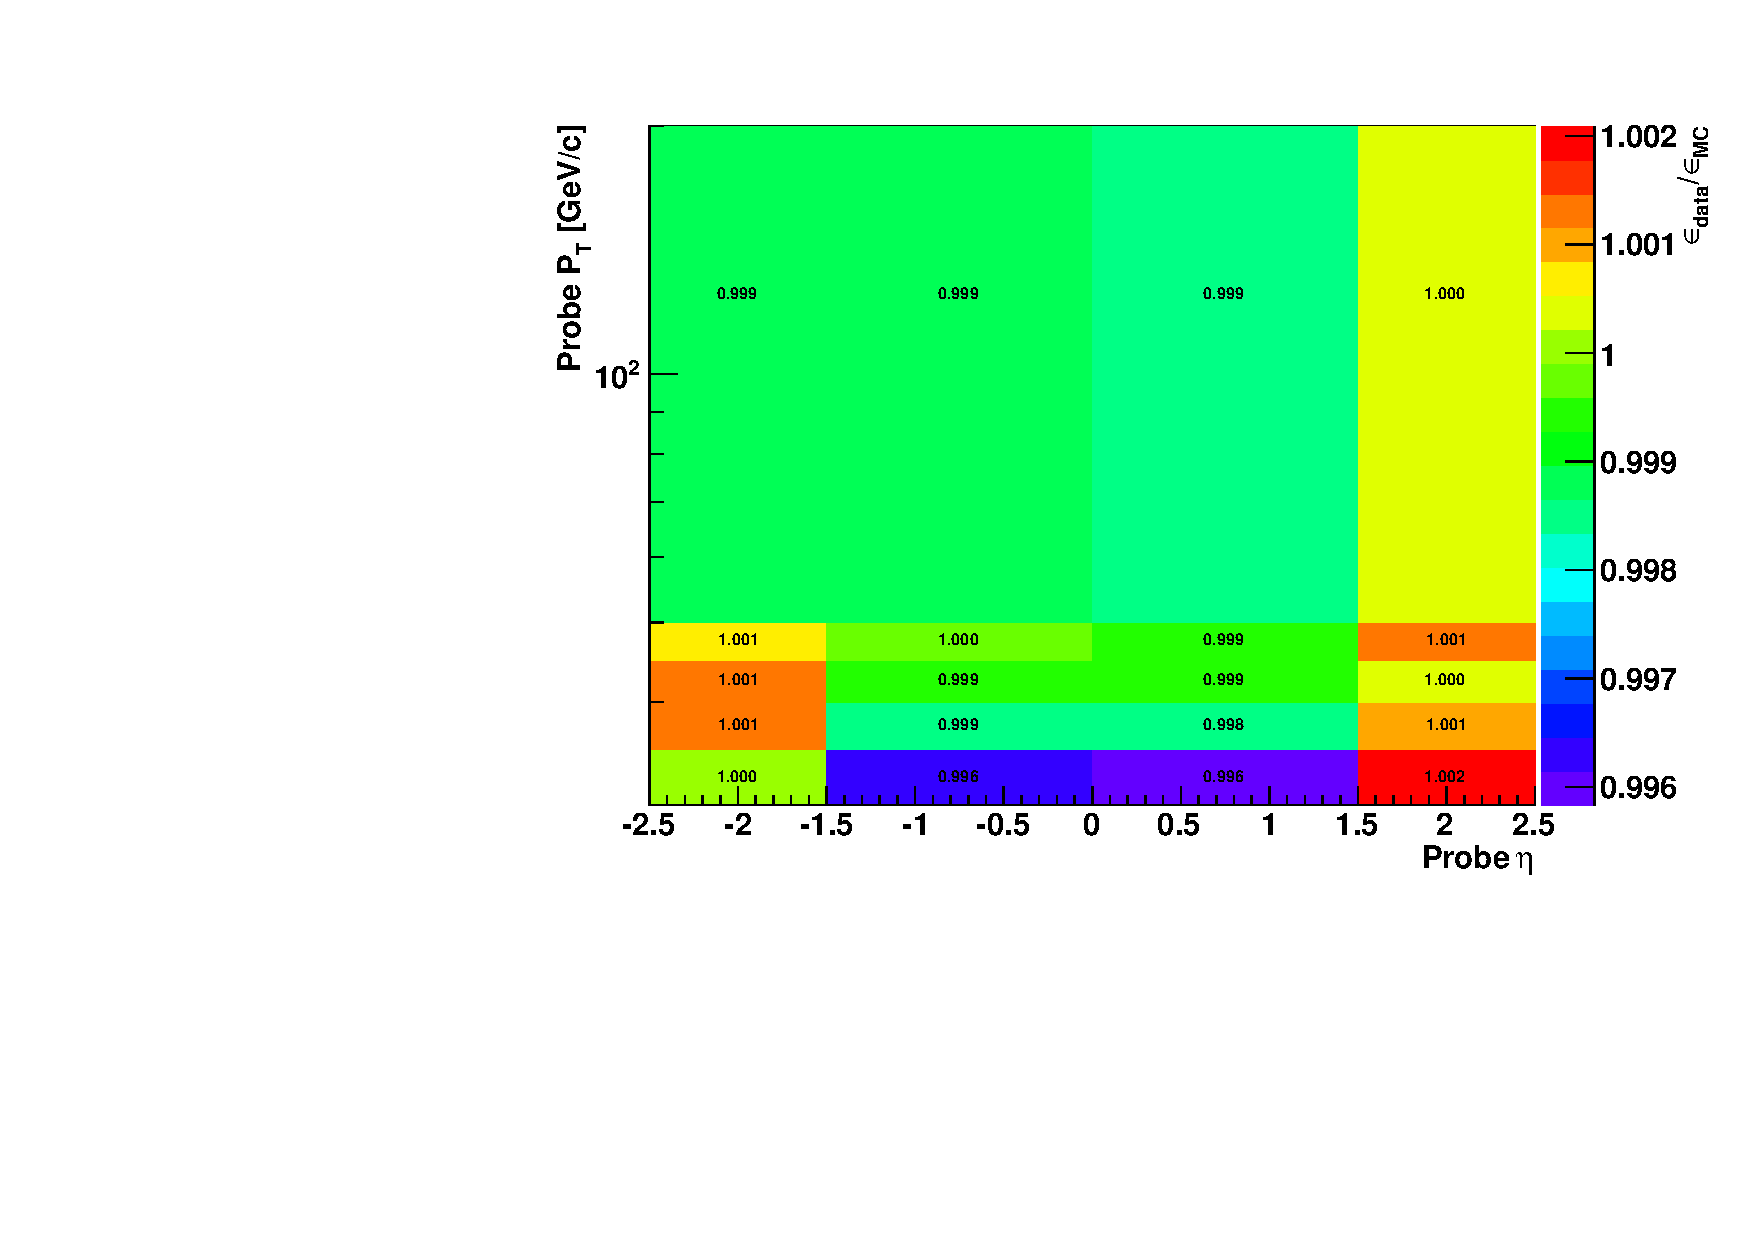
\includegraphics[width=0.32\textwidth]{figs/scaleFactor-Run2012ABC-SCToElectron.pdf}
  }
    \subfigure[]{
    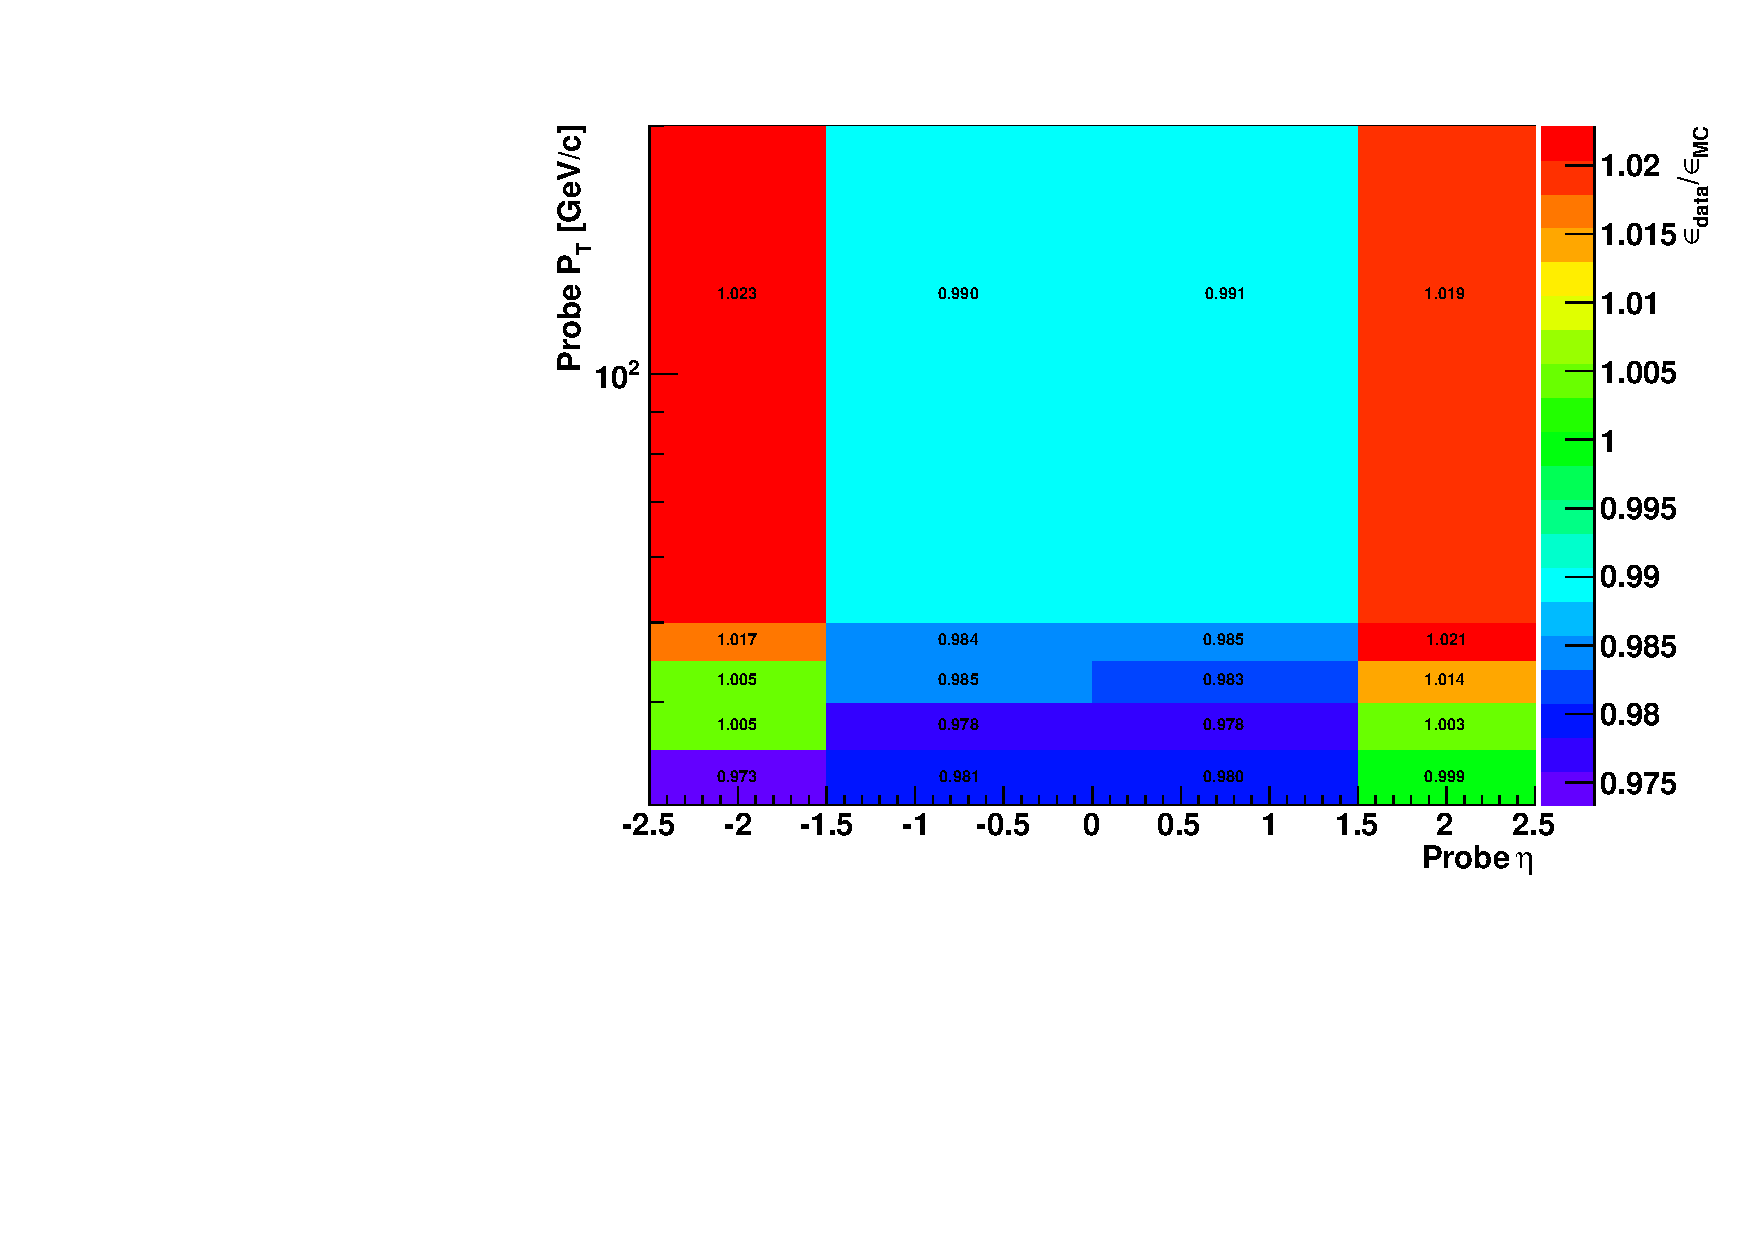
\includegraphics[width=0.32\textwidth]{figs/scaleFactor-Run2012ABC-GsfElectronToId.pdf}
  }
  \subfigure[]{
    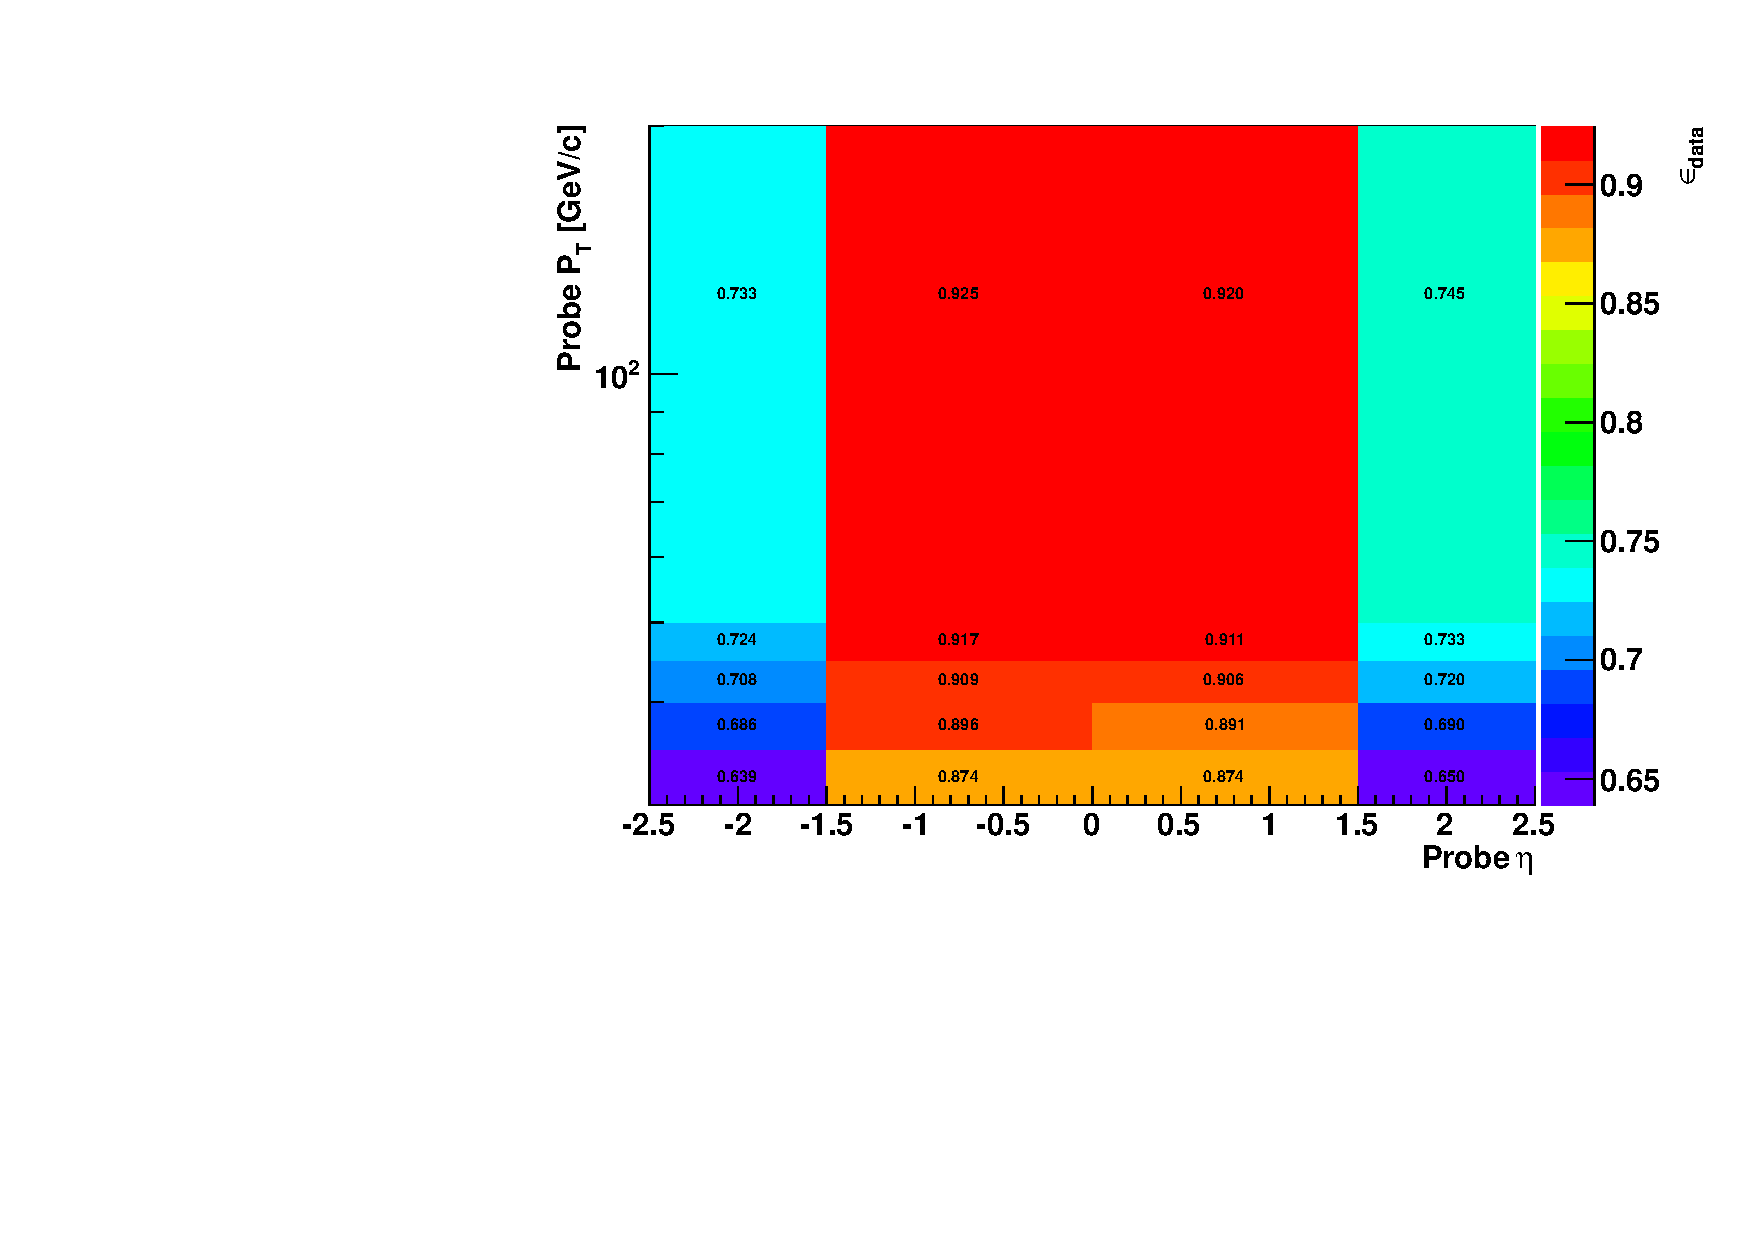
\includegraphics[width=0.32\textwidth]{figs/efficiency-Run2012ABC-WP80ToHLTEle.pdf}
  }
    \caption{Electron efficiency and data/MC scale factors for super-cluster to reconstructed electrons $\epsilon_{\textnormal{Reco}}$ (a),
    reconstructed to selected electrons $\epsilon_{\textnormal{Id}}$ (b) and selected to HLT electrons
      $\epsilon_{\textnormal{HLT}}$ (c).}
    \label{fig:eleEff}
  \end{center}
\end{figure}

\subsection{Muon efficiencies}\label{subsec:EffMu}

In the muon case, the reconstruction efficiency $\epsilon_{\textnormal{Reco}}$ describes the ability to reconstruct a Particle Flow muon starting with
a particle track and can be assumed to be one \cite{MUONPAS}. The identification efficiency $\epsilon_{\textnormal{Id}}$ gives an estimate for a
reconstructed muon to pass the offline selection criteria. It can be computed for both data and simulation and thus a scale factor being
the ratio of the two efficiencies is derived. \\
The trigger efficiency $\epsilon_{\textnormal{HLT}}$  is the fraction of selected muons fulfilling the HLT requirements and, since the HLT
requirement is dropped on the MC analysis, the efficiency computed on data is used directly to correct the MC event expectation.\\
The efficiency measurement is binned both in $\pt$ and $\eta$ of the probe muon covering the
relevant intervals (25, 30, 35, 40, 45, 50, 200)\GeVc in $\pt$ and (-2.1, -1.5, -1.0, -0.5, 0.0, 0.5, 1.0, 1.5, 2.1) in $\eta$. The resulting selection
and trigger efficiencies and scale factors are summarized in Table~\ref{tab:muonEff} and Figure~\ref{fig:muonEff}.

\begin{table}[htb]
\centering 
\scalebox{0.70}{
  \begin{tabular}{|c|c|c|c|c|c|}
  \hline
  $p_{\textnormal{T,min}}$ & $p_{\textnormal{T,max}}$ & $\eta_{\textnormal{min}}$ & $\eta_{\textnormal{max}}$ & $\epsilon_{\textnormal{ID,data}}$/$\epsilon_{\textnormal{ID,mc}}$ & $\epsilon_{\textnormal{HLT,data}}$ \\
  $[\GeVc]$         & $[\GeVc]$         &                     &                     &                             &                               \\
  \hline
  \hline
  25 & 30 & -2.1 & -1.5 & 0.992 $\pm$ 0.003 & 0.766 $\pm$ 0.003 \\
  25 & 30 & -1.5 & -1 & 0.987 $\pm$ 0.003 & 0.822 $\pm$ 0.003 \\
  25 & 30 & -1 & -0.5 & 0.990 $\pm$ 0.003 & 0.914 $\pm$ 0.002 \\
  25 & 30 & -0.5 & 0 & 0.984 $\pm$ 0.003 & 0.920 $\pm$ 0.002 \\
  25 & 30 & 0 & 0.5 & 0.985 $\pm$ 0.003 & 0.924 $\pm$ 0.002 \\
  25 & 30 & 0.5 & 1 & 0.992 $\pm$ 0.003 & 0.913 $\pm$ 0.002 \\
  25 & 30 & 1 & 1.5 & 0.991 $\pm$ 0.003 & 0.802 $\pm$ 0.003 \\
  25 & 30 & 1.5 & 2.1 & 0.995 $\pm$ 0.002 & 0.814 $\pm$ 0.003 \\
  30 & 35 & -2.1 & -1.5 & 0.991 $\pm$ 0.002 & 0.785 $\pm$ 0.002 \\
  30 & 35 & -1.5 & -1 & 0.988 $\pm$ 0.002 & 0.829 $\pm$ 0.002 \\
  30 & 35 & -1 & -0.5 & 0.988 $\pm$ 0.002 & 0.921 $\pm$ 0.002 \\
  30 & 35 & -0.5 & 0 & 0.984 $\pm$ 0.002 & 0.930 $\pm$ 0.001 \\
  30 & 35 & 0 & 0.5 & 0.985 $\pm$ 0.002 & 0.935 $\pm$ 0.001 \\
  30 & 35 & 0.5 & 1 & 0.990 $\pm$ 0.002 & 0.922 $\pm$ 0.002 \\
  30 & 35 & 1 & 1.5 & 0.987 $\pm$ 0.002 & 0.807 $\pm$ 0.002 \\
  30 & 35 & 1.5 & 2.1 & 0.995 $\pm$ 0.002 & 0.833 $\pm$ 0.002 \\
  35 & 40 & -2.1 & -1.5 & 0.992 $\pm$ 0.002 & 0.793 $\pm$ 0.002 \\
  35 & 40 & -1.5 & -1 & 0.987 $\pm$ 0.002 & 0.832 $\pm$ 0.002 \\
  35 & 40 & -1 & -0.5 & 0.991 $\pm$ 0.002 & 0.926 $\pm$ 0.001 \\
  35 & 40 & -0.5 & 0 & 0.986 $\pm$ 0.002 & 0.935 $\pm$ 0.001 \\
  35 & 40 & 0 & 0.5 & 0.986 $\pm$ 0.002 & 0.940 $\pm$ 0.001 \\
  35 & 40 & 0.5 & 1 & 0.991 $\pm$ 0.002 & 0.925 $\pm$ 0.001 \\
  35 & 40 & 1 & 1.5 & 0.989 $\pm$ 0.002 & 0.812 $\pm$ 0.002 \\
  35 & 40 & 1.5 & 2.1 & 0.994 $\pm$ 0.002 & 0.837 $\pm$ 0.002 \\
  40 & 45 & -2.1 & -1.5 & 0.994 $\pm$ 0.002 & 0.800 $\pm$ 0.002 \\
  40 & 45 & -1.5 & -1 & 0.987 $\pm$ 0.001 & 0.837 $\pm$ 0.002 \\
  40 & 45 & -1 & -0.5 & 0.992 $\pm$ 0.001 & 0.927 $\pm$ 0.001 \\
  40 & 45 & -0.5 & 0 & 0.986 $\pm$ 0.001 & 0.940 $\pm$ 0.001 \\
  40 & 45 & 0 & 0.5 & 0.987 $\pm$ 0.001 & 0.944 $\pm$ 0.001 \\
  40 & 45 & 0.5 & 1 & 0.991 $\pm$ 0.001 & 0.928 $\pm$ 0.001 \\
  40 & 45 & 1 & 1.5 & 0.991 $\pm$ 0.001 & 0.817 $\pm$ 0.002 \\
  40 & 45 & 1.5 & 2.1 & 0.996 $\pm$ 0.001 & 0.844 $\pm$ 0.002 \\
  45 & 50 & -2.1 & -1.5 & 0.993 $\pm$ 0.002 & 0.807 $\pm$ 0.002 \\
  45 & 50 & -1.5 & -1 & 0.987 $\pm$ 0.002 & 0.840 $\pm$ 0.002 \\
  45 & 50 & -1 & -0.5 & 0.990 $\pm$ 0.001 & 0.931 $\pm$ 0.001 \\
  45 & 50 & -0.5 & 0 & 0.988 $\pm$ 0.002 & 0.941 $\pm$ 0.001 \\
  45 & 50 & 0 & 0.5 & 0.987 $\pm$ 0.002 & 0.947 $\pm$ 0.001 \\
  45 & 50 & 0.5 & 1 & 0.992 $\pm$ 0.001 & 0.930 $\pm$ 0.001 \\
  45 & 50 & 1 & 1.5 & 0.991 $\pm$ 0.002 & 0.821 $\pm$ 0.002 \\
  45 & 50 & 1.5 & 2.1 & 0.995 $\pm$ 0.002 & 0.851 $\pm$ 0.002 \\
  50 & 200 & -2.1 & -1.5 & 0.991 $\pm$ 0.002 & 0.809 $\pm$ 0.002 \\
  50 & 200 & -1.5 & -1 & 0.987 $\pm$ 0.002 & 0.842 $\pm$ 0.002 \\
  50 & 200 & -1 & -0.5 & 0.992 $\pm$ 0.002 & 0.931 $\pm$ 0.001 \\
  50 & 200 & -0.5 & 0 & 0.987 $\pm$ 0.002 & 0.944 $\pm$ 0.001 \\
  50 & 200 & 0 & 0.5 & 0.989 $\pm$ 0.002 & 0.946 $\pm$ 0.001 \\
  50 & 200 & 0.5 & 1 & 0.992 $\pm$ 0.002 & 0.932 $\pm$ 0.001 \\
  50 & 200 & 1 & 1.5 & 0.993 $\pm$ 0.002 & 0.824 $\pm$ 0.002 \\
  50 & 200 & 1.5 & 2.1 & 0.996 $\pm$ 0.002 & 0.854 $\pm$ 0.002 \\
  \hline
  \end{tabular}}
\caption{Muon selection scale factors and HLT efficiencies. The errors are statistical only.} 
\label{tab:muonEff} 
\end{table}

\begin{figure}[t]
  \begin{center}
    \subfigure[]{
    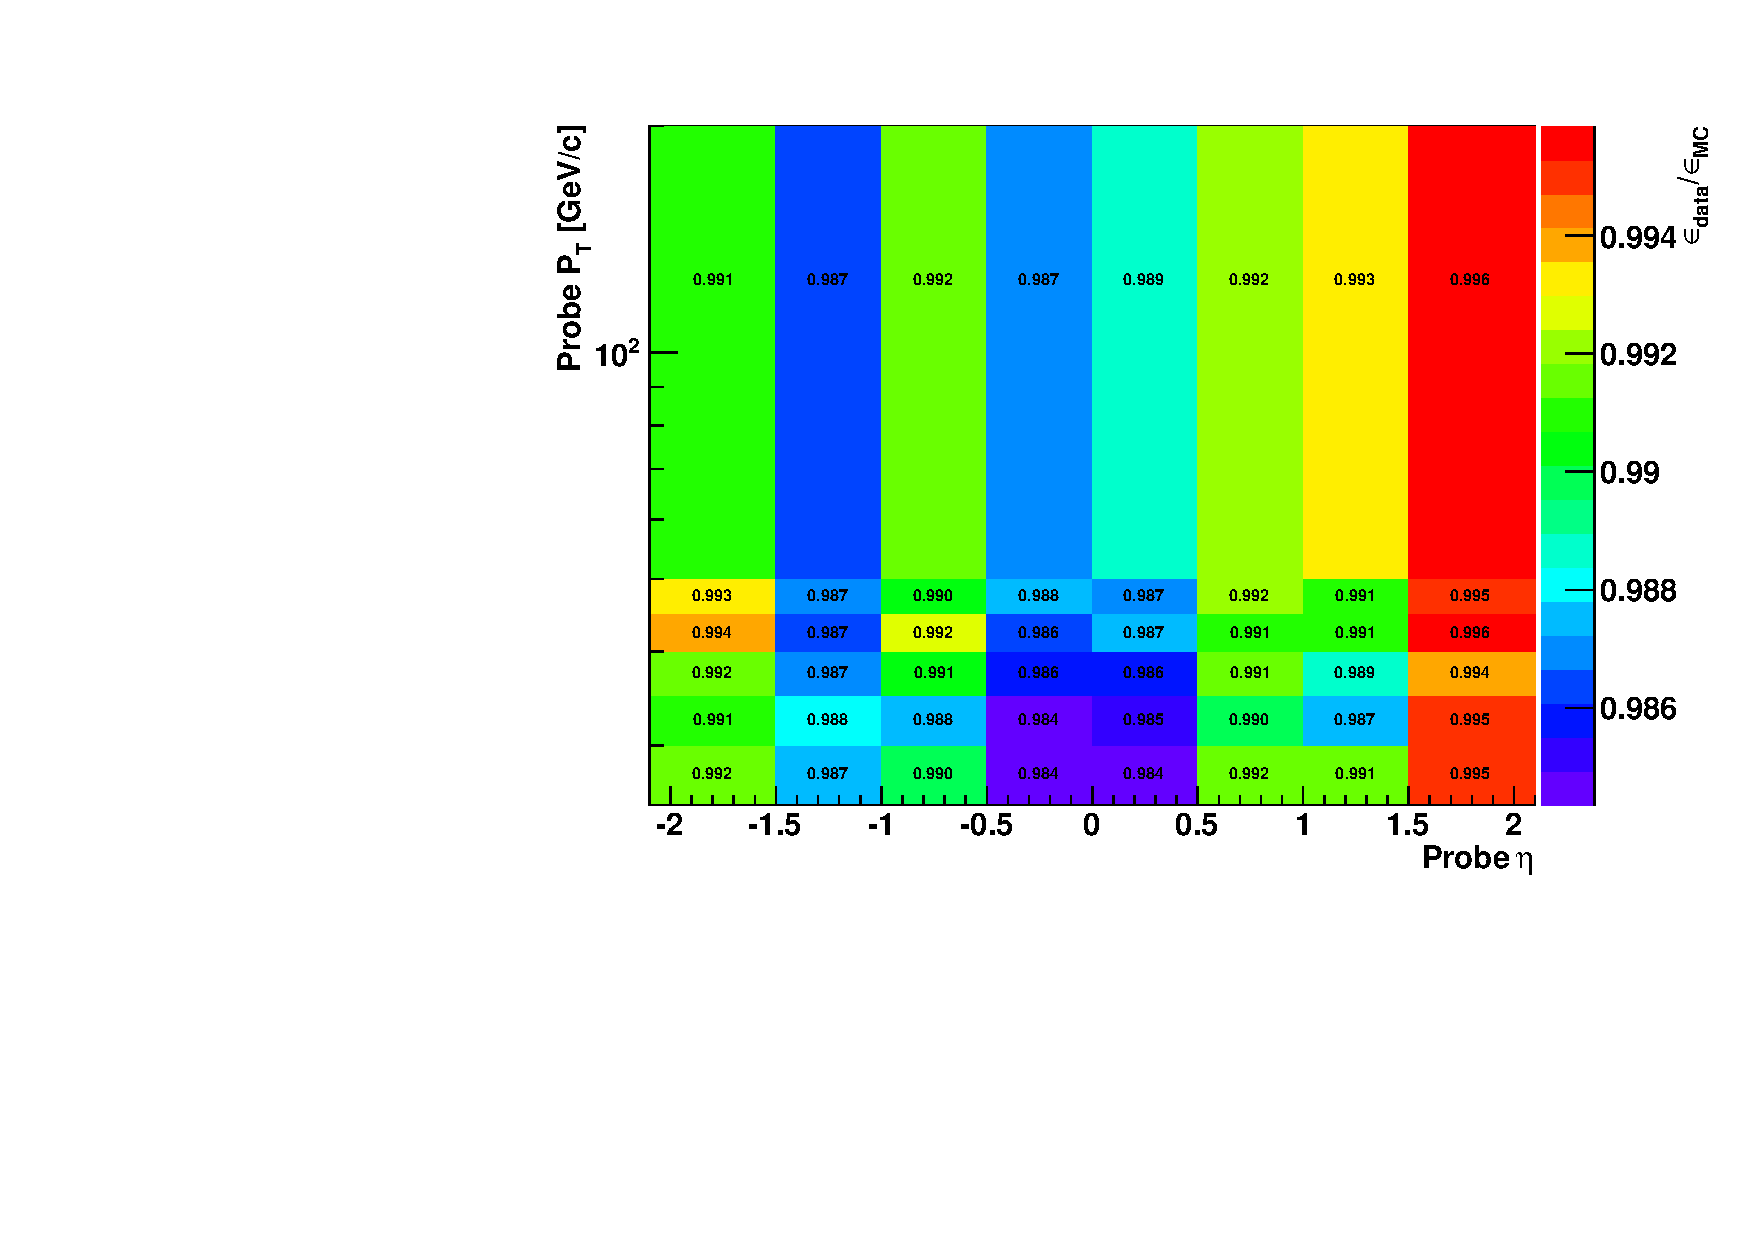
\includegraphics[width=0.47\textwidth]{figs/scaleFactor-Run2012ABC-RecoToIso.pdf}
  }
  \subfigure[]{
    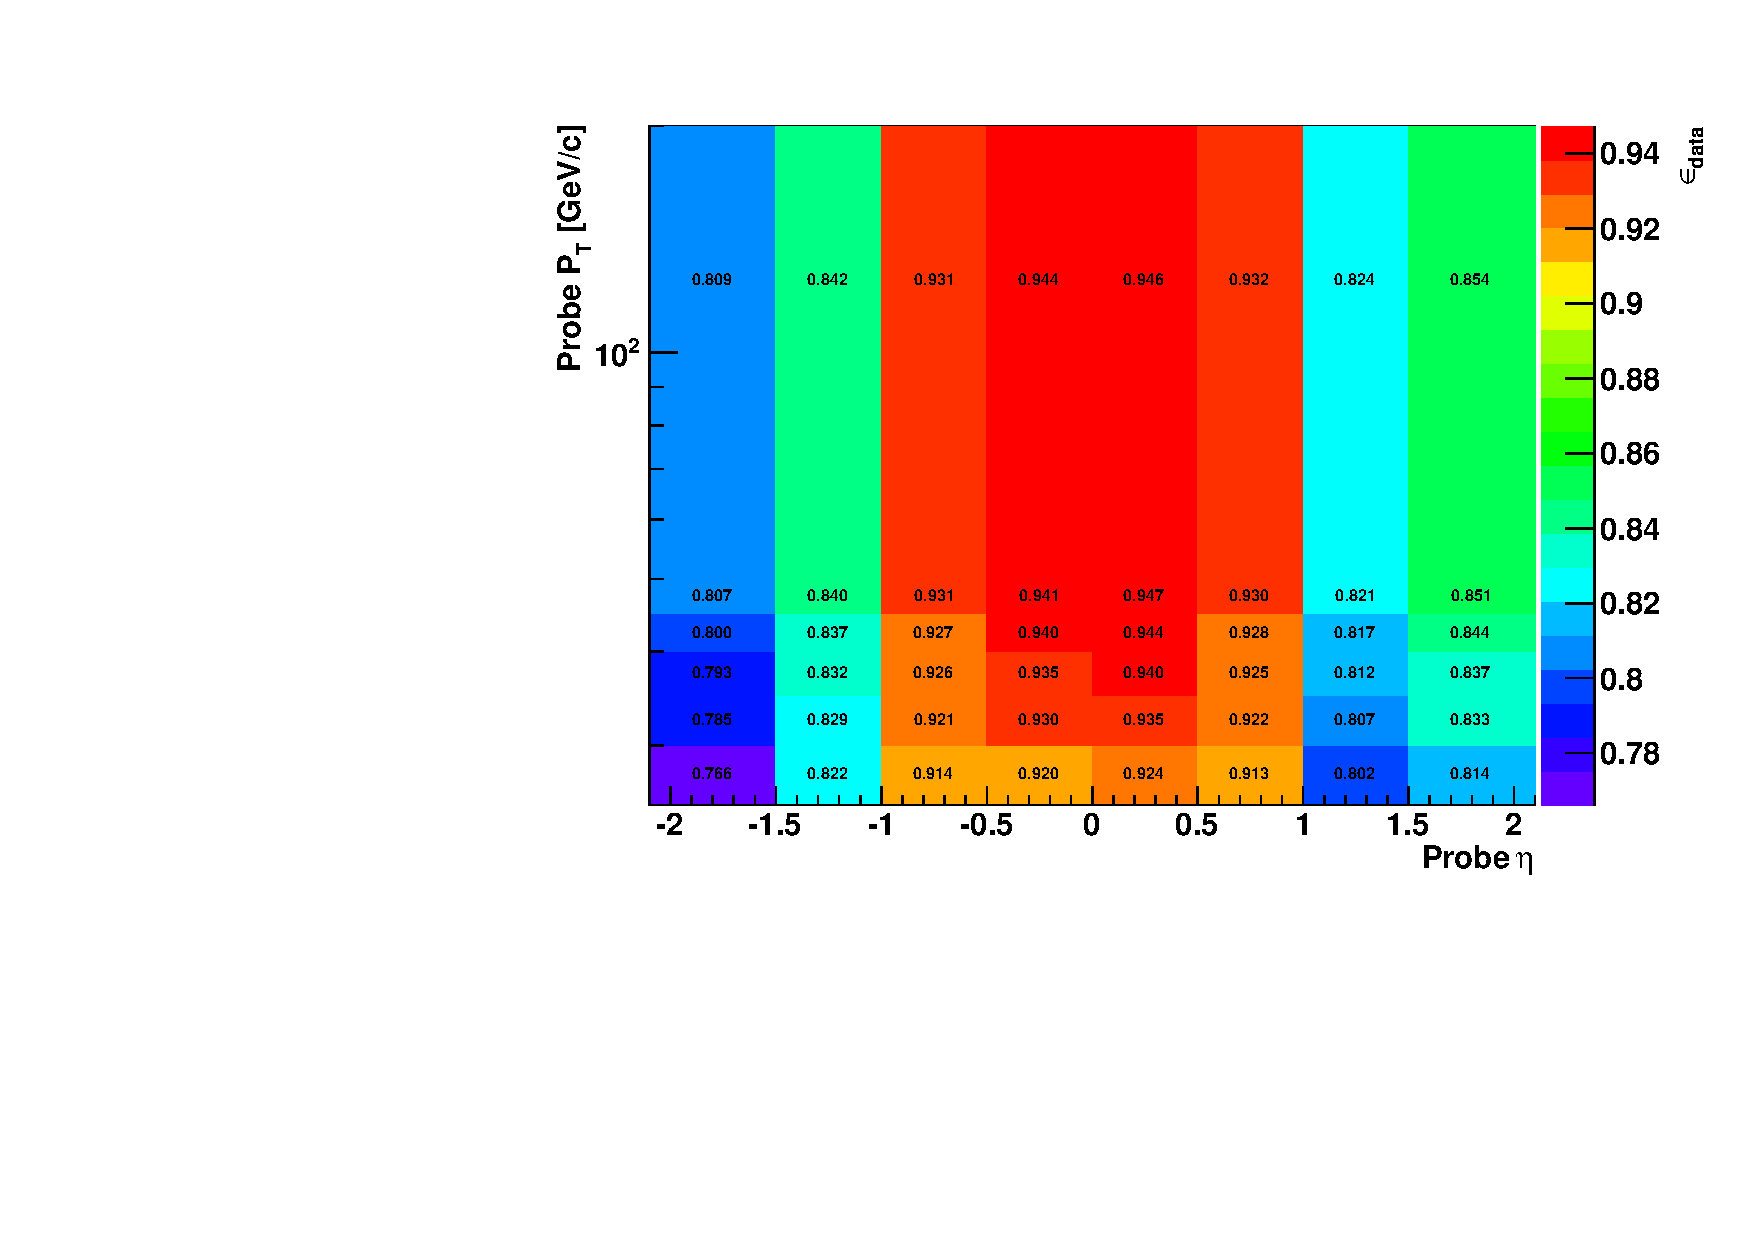
\includegraphics[width=0.47\textwidth]{figs/efficiency-Run2012ABC-IsoToIsoMuHLT.pdf}
  }
    \caption{Muon scale factors for reconstructed to selected muons $\epsilon_{\textnormal{ID,data}}$/$\epsilon_{\textnormal{ID,mc}}$ (a) and 
    efficiency for selected to HLT muons $\epsilon_{\textnormal{HLT,data}}$ (b).}
    \label{fig:muonEff}
  \end{center}
\end{figure}

%%%%%%%%%%%%%%%%%%%%%%%%%%%%%%%%%%%%%%%%%%%%%%%%%%%%%%%%%%%%%%%%%%%%
%%%%%%%%%%%%%%%%%%%%%%%%%%%%%%%%%%%%%%%%%%%%%%%%%%%%%%%%%%%%%%%%%%%%
\section{Effect of pileup}
\label{sec:pileup}
The presence of additional interactions, known as Pile-up (PU), is expected to affect
this analysis in the following ways:
%%%%%
\begin{itemize}
\item additional energy deposits from PU will be added to the jets from the main 
interaction
\item additional low $p_{T}$ jets composed of PU energy will be
added to the event
\item tracks and calorimetric towers from PU energy deposits will be
added to the isolation energy sum of the lepton, thus making isolation 
cuts less efficient.
\end{itemize}
%%%%%
Particle flow (PF) algorithms can be used to decrease the effects of pileup. 
Charged PF particles with tracks pointing to non-primary 
vertices are removed from the list of particles used to reconstruct jets. 
Neutral particles do not leave tracks, and therefore cannot be associated with
a vertex and removed. 

\par
Various techniques have been developed and centrally validated in CMS to 
alleviate the degradation in object reconstruction due to PU effects.
The present analysis makes full use of these improvements. 
The so-called Fastjet and L1-offset corrections remove the additional 
energy released in the event from PU interactions.
The charged particles coming from PU are removed prior to 
jet clustering by requiring that all the tracks come from the primary vertex. 
Similarly, for leptons we subtract from the isolation 
energy sum the pileup contribution from charged particles.
As a result of these corrections, 
the effect of pile-up reweighing in the analysis should be small.
In order to verify this hypothesis, the Fall11 Monte Carlo samples have 
been corrected, with a reweighing factor obtained from the comparison of 
the number of vertices in data and in Monte Carlo .
The effect of PU on the $m_{jj}$ shape from the W+jets Monte Carlo is 
shown in section~10 of CMS AN-2011/266 as well as in Fig.~\ref{fig:pu_MCcomp} for 8~TeV, in which the dijet mass distribution 
is shown before and after the PU correction. 
We conclude from these plots that the effect of pileup on the dijet mass
distributions is statistically insignificant.

%%%%%%%
\begin{figure}[h!] {\centering
\unitlength=0.33\linewidth
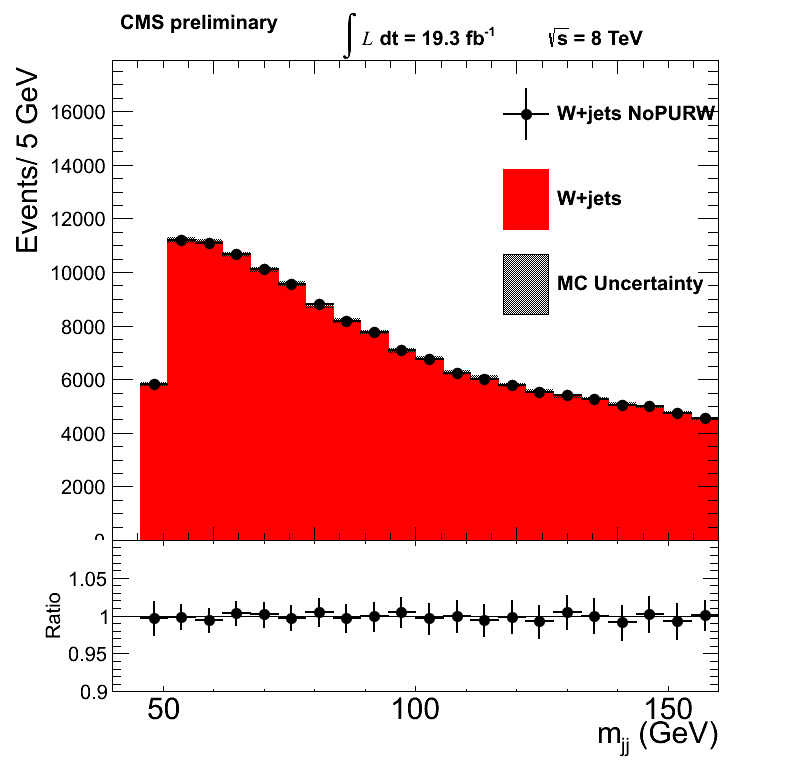
\includegraphics[width=0.48\textwidth]{figs/puchecks/mu_PUvsNoPUReweightingmjj.png}
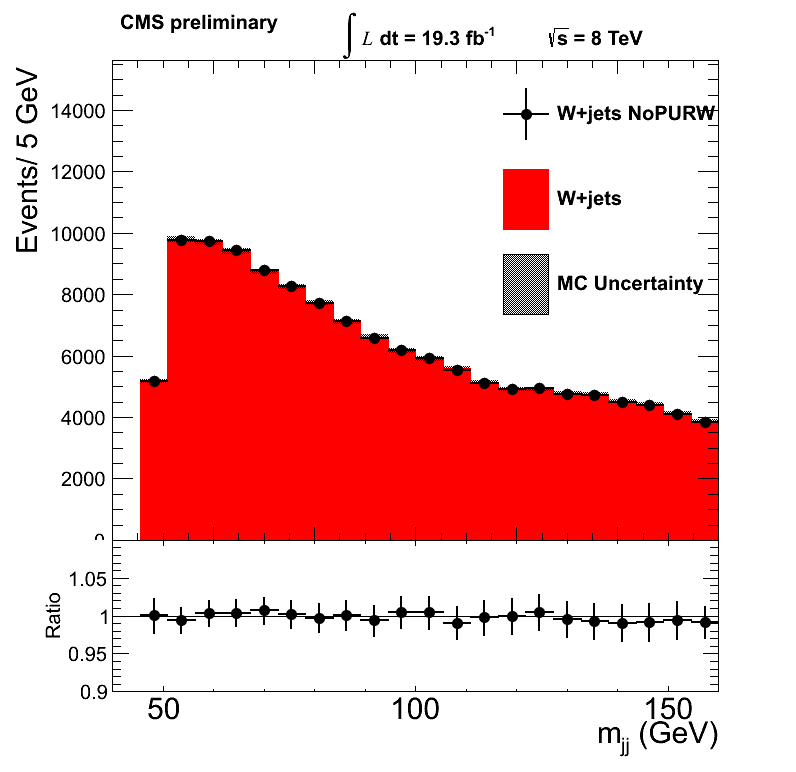
\includegraphics[width=0.48\textwidth]{figs/puchecks/el_PUvsNoPUReweightingmjj.png}
\caption{Difference in shape for the $m_{jj}$ distribution in the W+jets 
Monte Carlo, for muons (right) and electrons (left) with and without applying 
PU re-weighting according to the number of primary vertices in the event. 
The lower frame shows the difference in shape, 
after correcting for the different area of both distributions.
The ratio of the two distributions is consistent with unity.} 
\label{fig:pu_MCcomp}}
\end{figure}
%%%%%%%


We also compare the agreement between data and Monte Carlo as a function of PileUp. Specifically, the leading jet $p_T$, $m_{jj}$ (merged jet $p_T$, $m_J$) for the resolved (boosted) case comparisons are shown for low (NPV$<12$), medium ($12<$NPV$<18$) and high (NPV$>18$) PU scenarios are shown in Figs.~\ref{fig:pu_mjjLow}-\ref{fig:pu_mergedjetptHigh}. The profiles for three cases are consistent (within statistics).
%%%%%%%%%%%%%%%%%%%%%%%%%%%%
%%%%%%%
\begin{figure}[h!t]
  {\centering
    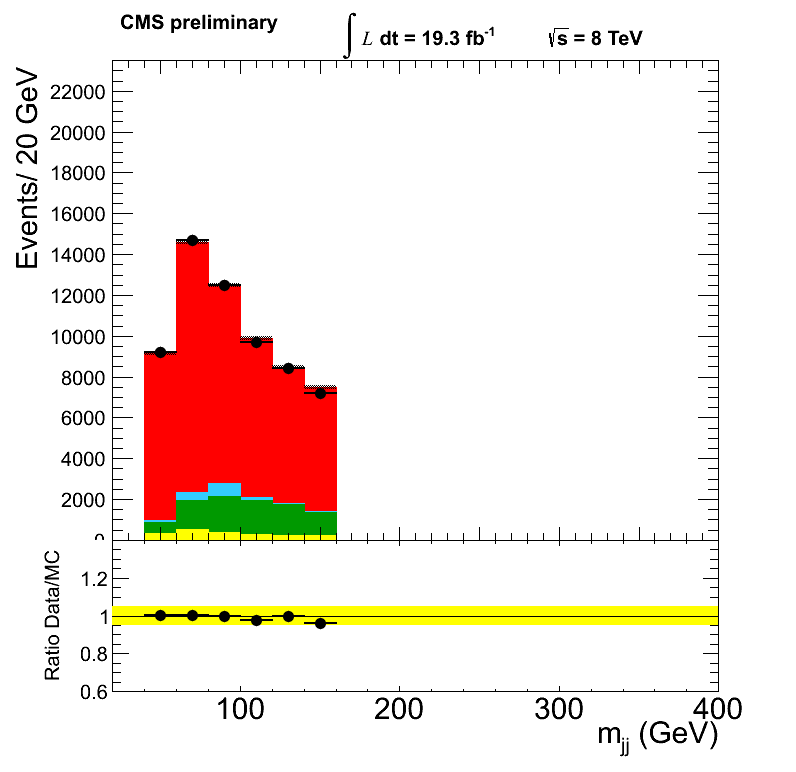
\includegraphics[width=0.49\textwidth]{figs/puchecks/mu_LowNPV_mjj.png}
    \includegraphics[width=0.49\textwidth]{figs/puchecks/el_LowNPV_mjj.png}
    \caption{Comparison of the distributions from data and MC of the
    dijet mass for muons (left) and electrons (right)
    in Low (NPV$<12$) PileUp dijet events.}
\label{fig:pu_mjjLow}}
\end{figure}
%%%%%%%
%%%%%%%
\begin{figure}[h!t]
  {\centering
    \includegraphics[width=0.49\textwidth]{figs/puchecks/mu_MedNPV_mjj.png}
    \includegraphics[width=0.49\textwidth]{figs/puchecks/el_MedNPV_mjj.png}
    \caption{Comparison of the distributions from data and MC of the
    dijet mass for muons (left) and electrons (right)
    in Medium ($12<$NPV$<18$) PileUp dijet events.}
\label{fig:pu_mjjMed}}
\end{figure}
%%%%%%%
%%%%%%%
\begin{figure}[h!t]
  {\centering
    \includegraphics[width=0.49\textwidth]{figs/puchecks/mu_HighNPV_mjj.png}
    \includegraphics[width=0.49\textwidth]{figs/puchecks/el_HighNPV_mjj.png}
    \caption{Comparison of the distributions from data and MC of the
    dijet mass for muons (left) and electrons (right)
    in High (NPV$>18$) PileUp dijet events.}
\label{fig:pu_mjjHigh}}
\end{figure}
%%%%%%%
%%%%%%% jetld
\begin{figure}[h!t]
  {\centering
    \includegraphics[width=0.49\textwidth]{figs/puchecks/mu_LowNPV_jetld_pt.png}
    \includegraphics[width=0.49\textwidth]{figs/puchecks/el_LowNPV_jetld_pt.png}
    \caption{Comparison of the distributions from data and MC of the
    leading jet $p_T$ for muons (left) and electrons (right)
    in Low (NPV$<12$) PileUp dijet events.}
\label{fig:pu_jetldLow}}
\end{figure}
%%%%%%%
%%%%%%%
\begin{figure}[h!t]
  {\centering
    \includegraphics[width=0.49\textwidth]{figs/puchecks/mu_MedNPV_jetld_pt.png}
    \includegraphics[width=0.49\textwidth]{figs/puchecks/el_MedNPV_jetld_pt.png}
    \caption{Comparison of the distributions from data and MC of the
    leading jet $p_T$ for muons (left) and electrons (right)
    in Medium ($12<$NPV$<18$) PileUp dijet events.}
\label{fig:pu_jetldMed}}
\end{figure}
%%%%%%%
%%%%%%%
\begin{figure}[h!t]
  {\centering
    \includegraphics[width=0.49\textwidth]{figs/puchecks/mu_HighNPV_jetld_pt.png}
    \includegraphics[width=0.49\textwidth]{figs/puchecks/el_HighNPV_jetld_pt.png}
    \caption{Comparison of the distributions from data and MC of the
    leading jet $p_T$ for muons (left) and electrons (right)
    in High (NPV$>18$) PileUp dijet events.}
\label{fig:pu_jetldHigh}}
\end{figure}
%%%%%%%
%%%%%%%%%%%%%%%%%%%%%%%%%%%%
%%%%%%%
\begin{figure}[h!t]
  {\centering
    \includegraphics[width=0.49\textwidth]{figs/puchecks/mu_LowNPV_GroomedJet_mass.png}
    \includegraphics[width=0.49\textwidth]{figs/puchecks/el_LowNPV_GroomedJet_mass.png}
    \caption{Comparison of the distributions from data and MC of the
    merged jet mass for muons (left) and electrons (right)
    in Low (NPV$<12$) PileUp boosted events.}
\label{fig:pu_GroomedJet_massLow}}
\end{figure}
%%%%%%%
%%%%%%%
\begin{figure}[h!t]
  {\centering
    \includegraphics[width=0.49\textwidth]{figs/puchecks/mu_MedNPV_GroomedJet_mass.png}
    \includegraphics[width=0.49\textwidth]{figs/puchecks/el_MedNPV_GroomedJet_mass.png}
    \caption{Comparison of the distributions from data and MC of the
    merged jet mass for muons (left) and electrons (right)
    in Medium ($12<$NPV$<18$) PileUp boosted events.}
\label{fig:pu_GroomedJet_massMed}}
\end{figure}
%%%%%%%
%%%%%%%
\begin{figure}[h!t]
  {\centering
    \includegraphics[width=0.49\textwidth]{figs/puchecks/mu_HighNPV_GroomedJet_mass.png}
    \includegraphics[width=0.49\textwidth]{figs/puchecks/el_HighNPV_GroomedJet_mass.png}
    \caption{Comparison of the distributions from data and MC of the
    merged jet mass for muons (left) and electrons (right)
    in High (NPV$>18$) PileUp boosted events.}
\label{fig:pu_GroomedJet_massHigh}}
\end{figure}
%%%%%%%
%%%%%%%
\begin{figure}[h!t]
  {\centering
    \includegraphics[width=0.49\textwidth]{figs/puchecks/mu_LowNPV_GroomedJet_pt_pr.png}
    \includegraphics[width=0.49\textwidth]{figs/puchecks/el_LowNPV_GroomedJet_pt_pr.png}
    \caption{Comparison of the distributions from data and MC of the
    merged jet $p_T$ for muons (left) and electrons (right)
    in Low (NPV$<12$) PileUp boosted events.}
\label{fig:pu_mergedjetptLow}}
\end{figure}
%%%%%%%
%%%%%%%
\begin{figure}[h!t]
  {\centering
    \includegraphics[width=0.49\textwidth]{figs/puchecks/mu_MedNPV_GroomedJet_pt_pr.png}
    \includegraphics[width=0.49\textwidth]{figs/puchecks/el_MedNPV_GroomedJet_pt_pr.png}
    \caption{Comparison of the distributions from data and MC of the
    merged jet $p_T$ for muons (left) and electrons (right)
    in Medium ($12<$NPV$<18$) PileUp boosted events.}
\label{fig:pu_mergedjetptMed}}
\end{figure}
%%%%%%%
%%%%%%%
\begin{figure}[h!t]
  {\centering
    \includegraphics[width=0.49\textwidth]{figs/puchecks/mu_HighNPV_GroomedJet_pt_pr.png}
    \includegraphics[width=0.49\textwidth]{figs/puchecks/el_HighNPV_GroomedJet_pt_pr.png}
    \caption{Comparison of the distributions from data and MC of the
    merged jet $p_T$ for muons (left) and electrons (right)
    in High (NPV$>18$) PileUp boosted events.}
\label{fig:pu_mergedjetptHigh}}
\end{figure}
%%%%%%%
%%%%%%%%%%%%%%%%%%%%%%%%%%%%

{\bf To account for differences in the number of pile-up events 
compared to the data, the Monte Carlo samples are re-weighted to 
have on-avearge the same pileup distribution.}


%%%%%%%%%%%%%%%%%%%%%%%%%%%%%%%%%%%%%%%%%%%%%%%%%%%%%%%%%%%%%%%%%%%%
%%%%%%%%%%%%%%%%%%%%%%%%%%%%%%%%%%%%%%%%%%%%%%%%%%%%%%%%%%%%%%%%%%%%
%%%%%%%%%%%%%%%%%%%%%%%%%%%%%%%%%%%%%%%%%%%%%%%%%%%%%%%%%%%%%%%%%%%%
%%%%%%%%%%%%%%%%%%%%%%%%%%%%%%%%%%%%%%%%%%%%%%%%%%%%%%%%%%%%%%%%%%%%
%%%%%%%%%%%%%%%%%%%%%%%%%%%%%%%%%%%%%%%%%%%%%%%%%%%%%%%%%%%%%%%%%%%%
%%%%%%%%%%%%%%%%%%%%%%%%%%%%%%%%%%%%%%%%%%%%%%%%%%%%%%%%%%%%%%%%%%%%
%%%%%%%%%%%%%%%%%%%%%%%%%%%%%%%%%%%%%%%%%%%%%%%%%%%%%%%%%%%%%%%%%%%%
\section{Data Driven QCD Estimation}
\label{sec:qcd}

A background from QCD multijet events comes from 3- or 4-jet events
with one jet passing the lepton criteria as a 'fake'. However, it is
not practical to generate sufficient MC to create a statistically
significant sample that passes the selection criteria. Therefore, we
rely on a data-driven approach in which the isolation-inverted samples
from data, which mirror the QCD background, are used instead.
Specifically, we perform a two-component simultaneous fit to data of
the MET distribution in order to obtain the fraction of QCD events in
the data; the two components are a data-based QCD sample and a
MC-based W+Jets sample.

The electron QCD sample is obtained by selecting events
in the data with the isolation $>0.3$ (default selection for loose
electrons uses Iso$_{el}<\sim0.2$).  In order to increase statistics
for the QCD sample we also relax the MET cut from 30~GeV to 20~GeV and
remove the restrictions on Electron MVA.
Fig.~\ref{fig:QCDISOCutsWmTShape} demonstrates that taking $Iso>0.3$
(rather than simply inverting the isolation cut), relaxing the MET as
well as the Electron MVA gives us a falling $W_{mT}$ spectrum (as
opposed to a signal-like one, which contains a peak near
$W_{mT}=$80~GeV). The MC W+Jets and target data samples are obtained by
applying the default cuts (Sec~\ref{sec:firstStep}).

The fraction of QCD events in data is then obtained from a
fit to the MET distribution, with the normalizations for two components (
W+jets and QCD) free to float.
The results for the electrons are shown in Figure~\ref{fig:QCDTemplateFit_MET}. 
However, we inherently have a smaller sample of 
QCD events for the muons. Their relative fraction
is expected to be $<$1\% ({\it e.g.} 0.2\% in 7~TeV data, AN-11-110).
Likewise, the multijet contribution is suppressed in btagged as well as merged configuration and is highly correlated with the V+Jets background.
We do not require an independent model of the QCD event in the electron btagged, electron boosted and all muon configurations.

For the electron dijet anti-btagged case we implement the above approach. The final fraction of QCD events in data, after accounting for the change in accepatance due to the MET cut,
is $18.6\pm 0.2\%$. We conservatively assume a 50\% uncertainty on the QCD yield when fitting the data (Section~\ref{sec:mjj_fit}).

%Due to this assumption and to account for po crepancies in template modeling, a very
%large uncertainty is conservatively assumed. The final fraction of QCD
%events in data, after accounting for the change in accepatance due to the MET cut,
%is given in Table~\ref{tab:qcdfrac}.

%%%%%%%%%%%%%%%%%%%%%%%%%%%%%
%\begin{table}[bthp]
%\begin{center}
%  \begin{tabular}{l c}
%    \hline  \hline
%     & 2 jets \\
%    \hline  
%    electron  & 18.6 $\pm$ 0.2\% \\
%    muon      & 0.2 $\pm$ 0.4\% \\
%    \hline  \hline
%  \end{tabular}
%\end{center}
%\caption{\label{tab:qcdfrac} Estimates of the percentage of QCD in data (and
%the fit uncertainty) for the muon and electron datasets after selection.}
%\end{table}

%\subsection{QCD Uncertainties}
%\label{sec:qcd_Uncertainty}
%%%%%%%%%%%%%%%%%%%%%%%%%%%%%

%When performing the $m_{jj}$ fit the QCD yield
%is Gaussian-constrained with a mean given by the value shown in
%Table~\ref{tab:qcdfrac}.
%In the case of electrons, the error on the QCD fraction
%is small and we (conservatively) estimate
%the uncertainty to be one half of the expected value. For muons the
%uncertainty is the error on the relative fraction (i.e.,
%0.4\%).
%When obtaining the result for the sum of electron and muon data, the uncertainties
%are combined using the standard error propagation machinery.


\subsection{Cross-Checks}

In order to ensure that our inverted selection provides a consistent representation of
QCD events,
we fit the QCD with a Rayleigh Function: $xe^{-x^2/2(\sigma_0+\sigma_1x)^2}$,
used during the inclusive cross section measurements~\cite{WZCMS:2010}.
As can be seen from Fig.~\ref{fig:QCDMETRayleighFit},
the function accurately fits the overall shape as well as the parameter
corresponding to the intrinsic MET resolution ($\sigma_0\simeq 12$~GeV).

In addition we compare the above procedure to the fit with the remaining backgrounds included by
\begin{itemize}
\item Fixing the relative ratios based on the expected cross sections and fitting with the combination, instead of W+Jets. The resulting fraction of QCD (after correcting for MET acceptance) is $0.160\pm 0.002$.
\item Fixing the additional backgrounds to their expected values and only allowing W+Jets (and QCD) to float during the fit. The resulting fraction of QCD (after correcting for MET acceptance) is $0.156\pm 0.002$.
\end{itemize}
The results (Fig.~\ref{fig:QCDTemplateFit_MET_AllBkgds}) are consistent with the default approach.

We also examine the impact of the QCD selection cuts on W+Jets and $t\bar{t}$ MC events. The comparison is shown in Fig.~\ref{fig:QCDSelectionDataVsNonQCDMC}. The selection procedure does not significantly alter the shapes of the non-QCD distributions ({\it i.e} we retain the peak near $W_{mT}=$80~GeV and observe a broad resonance, rather than an exponentially falling spectrum, in the MET), which remain distinct from multijet events. There is no evidence that the data sideband contains a significant fraction of non-QCD events. 


%%%%%%%%%%%%%%%%%%%%%%%%%%%%
%%%%%%%
\begin{figure}[h!] {\centering
\unitlength=0.33\linewidth
\includegraphics[width=0.90\textwidth]{figs/qcd/TemplateFit19p2fbQCD_MET_el2j.png}
%\put(-0.80,0.0){(a)}
%\unitlength=0.33\linewidth
%\includegraphics[width=0.48\textwidth]{figs/2012_QCD/TemplateFit_MET_mu3j.pdf}
%\put(-0.80,0.0){(b)} \\
%\unitlength=0.33\linewidth
%\includegraphics[width=0.48\textwidth]{figs/2012_QCD/TemplateFit_MET_el2j.pdf}
%\put(-0.80,0.0){(c)}
%\unitlength=0.33\linewidth
%\includegraphics[width=0.48\textwidth]{figs/2012_QCD/TemplateFit_MET_el3j.pdf}
%\put(-0.80,0.0){(d)}
\caption{MET distributions fit to the QCD and W$jj$ templates for electrons.}
\label{fig:QCDTemplateFit_MET}
}
\end{figure}
%%%%%%%
%%%%%%%
\begin{figure}[h!] {\centering
\unitlength=0.33\linewidth
\includegraphics[width=0.90\textwidth]{figs/qcd/RaileighFitQCD_19p2fb_el2j.png}
\caption{QCD MET distribution fitted with a Rayleigh Function.}
\label{fig:QCDMETRayleighFit}
}
\end{figure}
%%%%%%%
%%%%%%%
\begin{figure}[h!] {\centering
\unitlength=0.33\linewidth
\includegraphics[width=0.90\textwidth]{figs/qcd/El2J_19p2fb_CutComparison_WmT.png}
% \put(-0.80,0.0){(a)}
% \unitlength=0.33\linewidth
% \includegraphics[width=0.48\textwidth]{figs/2012_QCD/ISOShapeComp_WmT_mu3j_g01vg02.pdf}
% \put(-0.80,0.0){(b)} \\
% \unitlength=0.33\linewidth
% \includegraphics[width=0.48\textwidth]{figs/2012_QCD/ISOShapeComp_WmT_el2j_g01vg02.pdf}
% \put(-0.80,0.0){(c)}
% \unitlength=0.33\linewidth
% \includegraphics[width=0.48\textwidth]{figs/2012_QCD/ISOShapeComp_WmT_el3j_g01vg02.pdf}
% \put(-0.80,0.0){(d)}
\caption{ QCD W transverse mass shapes with Iso$>0.3$, MET$>20$ and no Electron MVA cut vs inverted loose isolation, MET$>30$ and loose Electron MVA cuts.}
\label{fig:QCDISOCutsWmTShape}
}
\end{figure}
%%%%%%%
%%%%%%%
\begin{figure}[h!] {\centering
\unitlength=0.33\linewidth
\includegraphics[width=0.48\textwidth]{figs/qcd/TemplateFit19p2fb_MET_AllBkgds_el2j.png}
\put(-0.80,0.0){(a)}
\unitlength=0.33\linewidth
\includegraphics[width=0.48\textwidth]{figs/qcd/TemplateFit19p2fb_MET_AllBkgdsFixNonWpJ_el2j.png}
\put(-0.80,0.0){(b)}
\caption{ Electron MET distribution fit with: (a) fractions of the non QCD processes fixed relative to each other and the overall coefficient allowed to float (b) the additional backgrounds (i.e. processes which are not W+Jets or QCD) fixed to their expected yields and W+Jets (as well as QCD) fraction allowed to float. The resultant fraction of QCD events is consistent with the default approach (Fig.~\ref{fig:QCDTemplateFit_MET}).}
\label{fig:QCDTemplateFit_MET_AllBkgds}}
\end{figure}
%%%%%%%
%%%%%%%
\begin{figure}[h!] {\centering
\unitlength=0.33\linewidth
\includegraphics[width=0.48\textwidth]{figs/qcd/El2J_11p9fb_QCDvsMC_WmT.png}
\put(-0.80,0.0){(a)}
\unitlength=0.33\linewidth
\includegraphics[width=0.48\textwidth]{figs/qcd/El2J_11p9fb_QCDvsMC_MET.png}
\put(-0.80,0.0){(b)}
\caption{ Data, W+Jets MC and $t\bar{t}$ MC events with Iso$>0.3$, MET$>20$ and no Electron MVA cut for (a) $W_{mT}$ (b) MET. The shapes are distinct and there is no evidence of contamination in (what should be) data sideband multijet events.}
\label{fig:QCDSelectionDataVsNonQCDMC}}
\end{figure}
%%%%%%%


%%%%%%%%%%%%%%%%%%%%%%%%%%%%%%%%%%%%%%%%%%%%%%%%%%%%%%%%%%%%%%%%%%
%%%%%%%%%%%%%%%%%%%%%%%%%%%%%%%%%%%%%%%%%%%%%%%%%%%%%%%%%%%%%%%%%%
%%%%%%%%%%%%%%%%%%%%%%%%%%%%%%%%%%%%%%%%%%%%%%%%%%%%%%%%%%%%%%%%%%

\clearpage
\section{W+jets Background}
\label{sec:wjetsBackground}

In order to get a good description of the W+jets shape in data, the
simulation needs to describe well both the matrix elements for the
hard processes, and the subsequent development of the hard partons
into jets of hadrons.  However, no factorization theorem exists to
rigorously separate these two components.  A given (n + 1)-jet event
can be obtained in two ways: from the collinear/soft-radiation
evolution of an appropriate (n + 1)-parton final state, or from an
n-parton configuration where hard, large-angle emission during its
evolution leads to the extra jet.  A factorization scheme defines, on
an event-by-event basis, which of the two paths should be followed.
The two relevant parameters defining such a scheme are: the
factorization/renormalization scale $q^2$ and the matrix element -
parton shower matching threshold.  Optimized values of these
parameters should give the best possible approximation to the W+jets
kinematics for a given fixed-order calculation.  We know that the
physics has to be independent of the relative contributions of the two
components.

The CMS MadGraph W+jets production uses MLM matching
\cite{Hoche:2006ph} with $k_T$ jets.  The default matching threshold
is 10~GeV (i.e., if the parton $p_{T}$ is greater than 10~GeV, then it
is assumed to have originated from the hard scattering process and
contributes to the matrix element calculation; if the parton $p_{T}$
is less than 10~GeV then it is assumed to come from the parton
shower).  The factorization/renormalization scale $q^2$ corresponds to
the ``transverse mass'' of the W boson plus the hard jets: $\sqrt{M_W^2 + p_{T, W}^2 + \Sigma p_{T,j}^2}$.

\subsection{Factorization/renormalization scale and matrix element - parton shower matching threshold}
\label{sec:wjetsShapeMatchingQ2}

To perform studies of the uncertainty due to the choice of the $q^2$
and matching scales, alternative MadGraph W+jets samples are produced
in which the corresponding scales are changed by a factor of 2. Thus,
we have ``matching-up'', ``matching-down'', ``scale-up'', and
``scale-down'' samples, each yielding an $m_{jj}$ distribution, or
template. In order to compensate for limited statistics in the centrally generated samples
additional MadGraph Monte Carlo is produced locally with (the majority of) selection cuts applied at the generation level.
The approach significantly reduces the amount of MC required, though running the full detector simulation remaings a computing intensive process. In the end we generate enough events to effectively double the size of the samples and use the combination of local plus central ones, added with equal weights, in subsequent studies.

First, we attempt to follow the 7~TeV approach by using our samples to find an optimum MC template
$\mathcal{F}_{W+\text{jets}}$,
%%\[
\begin{equation}
\mathcal{F}_{W+\text{jets}} = \sum_\alpha f_\alpha \mathcal{G}_\alpha\, + (1-\sum_\alpha f_\alpha)\times\mathcal{G}_\text{nominal},
\label{eqn:wjetsShapeMatchingQ2}
\end{equation}
%%\]
where $\alpha \in
\{\text{matchingUp,~matchingDown,~scaleUp,~scaleDown}\}$,
$\mathcal{G}_\text{nominal}$ is the template from the default MadGraph
generation and $\mathcal{G}_\alpha$ is the template from the specified
sample.  We define a 2D coordinate system in scale and matching.  The
origin corresponds to the default MadGraph sample.  To move in the
positive scaleUp direction, one sets $f_\text{scaleDown}=0$ and
increases $f_\text{scaleUp}$. To move in the negative scaleUp
direction, one sets $f_\text{scaleUp}=0$ and increases
$f_\text{scaleDown}$.  The same is true for the matching samples.  We
allow the relative contributions from these templates to float in our
fit.  This lets the data determine the best W+jets shape and the
uncertainties on these parameters is automatically propagated to the
uncertainties on the yields.


\subsection{Monte Carlo Template Fit}

We follow the usual approach (described in section~\ref{sec:mjj_fit}) obtaining the diboson signal yield from an unbinned maximum
likelihood fit to the dijet invariant mass distribution in the data. The exctracted fraction (of the expected Standard Model diboson yield) is $1.74\pm 0.18$ ($2.11\pm 0.26$) in the muon (electron) channel. Likewise, the fit results (Figs.~\ref{fig:mjjfit_MCTemplate_mu},~\ref{fig:mjjfit_MCTemplate_el}) show a mismatch between the MC fit output and the data along with the corresponding bias in the pull distributions.

%%%%%%%%%%%%%%%%%%%%
\begin{figure}[h!]
  {\centering
    \includegraphics[width=0.49\textwidth]{figs/mjjfit/DibosonMCTemplatelnujj_muon_Stacked.png}
    \includegraphics[width=0.49\textwidth]{figs/mjjfit/DibosonMCTemplatelnujj_muon_Subtracted.png}
    \includegraphics[width=0.49\textwidth]{figs/mjjfit/DibosonMCTemplatelnujj_muon_Pull.png}
    \caption{Distribution of the W-jet invariant mass for the dijet (anti-btagged) 2+ jet events in muon data and fit shapes: 
      (upper left) All background components stacked together, 
      (upper right) unstacked, (lower left) [Data minus all backgrounds except diboson],  
      (lower right) normalized residual between data and MC. The vertical dotted lines
      indicate the mass interval excluded from the fit. The shape templates for each component are taken directly from Monte Carlo.}
    \label{fig:mjjfit_MCTemplate_mu}}
\end{figure}
%%%%%%%%%%%%%%%%%%%%
%%%%%%%%%%%%%%%%%%%%
\begin{figure}[h!]
  {\centering
    \includegraphics[width=0.49\textwidth]{figs/mjjfit/DibosonMCTemplatelnujj_electron_Stacked.png}
    \includegraphics[width=0.49\textwidth]{figs/mjjfit/DibosonMCTemplatelnujj_electron_Subtracted.png}
    \includegraphics[width=0.49\textwidth]{figs/mjjfit/DibosonMCTemplatelnujj_electron_Pull.png}
    \caption{Distribution of the W-jet invariant mass for the dijet (anti-btagged) 2+ jet events in electron data and fit shapes: 
      (upper left) All background components stacked together, 
      (upper right) unstacked, (lower left) [Data minus all backgrounds except diboson],  
      (lower right) normalized residual between data and MC. The vertical dotted lines
      indicate the mass interval excluded from the fit. The shape templates for each component are taken directly from Monte Carlo.}
    \label{fig:mjjfit_MCTemplate_el}}
\end{figure}
%%%%%%%%%%%%%%%%%%%%


\subsection{Convolved Monte Carlo Template Fit}
\label{sec:convolvedMCfit}

Next, we include the resolution effects directly in our fit (rather than treating them as a separate systematics). We take the gaussian resolution function, obtained from fits to the top control sample (section~\ref{sec:convolvedMCfit}), convolve it with the MC templates and repeat the fit. The results are shown in Figs.~\ref{fig:mjjfit_ConvolvedMCTemplate_mu},~\ref{fig:mjjfit_ConvolvedMCTemplate_el} with the extracted fraction (of the expected Standard Model diboson yield) of $1.71\pm 0.18$. The plots show a mismatch between MC fit output and the data along with the corresponding bias in the pull distributions. Accounting for resolution effects has a minimal impact on the fitting procedure. The above approach is inadequate for modeling the dijet mass distribution in the full 8~TeV CMS dataset.

%%%%%%%%%%%%%%%%%%%%
\begin{figure}[h!]
  {\centering
    \includegraphics[width=0.49\textwidth]{figs/mjjfit/DibosonConvolvedMCTemplatelnujj_muon_Stacked.png}
    \includegraphics[width=0.49\textwidth]{figs/mjjfit/DibosonConvolvedMCTemplatelnujj_muon_Subtracted.png}
    \includegraphics[width=0.49\textwidth]{figs/mjjfit/DibosonConvolvedMCTemplatelnujj_muon_Pull.png}
    \caption{Distribution of the W-jet invariant mass for the dijet (anti-btagged) 2+ jet events in muon data and fit shapes: 
      (upper left) All background components stacked together, 
      (upper right) unstacked, (lower left) [Data minus all backgrounds except diboson],  
      (lower right) normalized residual between data and MC. The vertical dotted lines
      indicate the mass interval excluded from the fit. The shape templates for each component are taken directly from Monte Carlo.}
    \label{fig:mjjfit_ConvolvedMCTemplate_mu}}
\end{figure}
%%%%%%%%%%%%%%%%%%%%
%%%%%%%%%%%%%%%%%%%%
\begin{figure}[h!]
  {\centering
    \includegraphics[width=0.49\textwidth]{figs/mjjfit/DibosonConvolvedMCTemplatelnujj_electron_Stacked.png}
    \includegraphics[width=0.49\textwidth]{figs/mjjfit/DibosonConvolvedMCTemplatelnujj_electron_Subtracted.png}
    \includegraphics[width=0.49\textwidth]{figs/mjjfit/DibosonConvolvedMCTemplatelnujj_electron_Pull.png}
    \caption{Distribution of the W-jet invariant mass for the dijet (anti-btagged) 2+ jet events in electron data and fit shapes: 
      (upper left) All background components stacked together, 
      (upper right) unstacked, (lower left) [Data minus all backgrounds except diboson],  
      (lower right) normalized residual between data and MC. The vertical dotted lines
      indicate the mass interval excluded from the fit. The shape templates for each component are taken directly from Monte Carlo.}
    \label{fig:mjjfit_ConvolvedMCTemplate_el}}
\end{figure}
%%%%%%%%%%%%%%%%%%%%



\clearpage
\section{Modeling Individual Processes}
\label{sec:individualProcesses}
\subsection{V+jets Background Shape}
\label{sec:wjetsShape}

Because of inadequate statistics in the V+jets MC and the overall poor
agreement between V+jets MC and many data distibutions, we employ an
empirical description of the V+jets shape for the default MadGraph sample, which consists of W+jets and Drell Yan events combined based on their predicted cross-sections(Table~\ref{tab:mjj_shapes_and_normalization}). In the dijet regime this description is 2-parameter power law, modulated by the error function corresponding to a kinematic turnon, for the anti-btagged events:
\begin{equation}
  \mathcal{F}_{V+\text{jets}} = \text{erf}(m_{jj}; m_0, \sigma)\times\left[(m_{jj})^{-\alpha-\beta\ln(m_{jj}/\sqrt{s})}\right]
\end{equation}
and a simple power law (modulated by the error function) for the btagged events:
\begin{equation}
  \mathcal{F}_{V+\text{jets}} = \text{erf}(m_{jj}; m_0, \sigma)\times\left[(m_{jj})^{-\alpha}\right]\,,
\end{equation}
where $m_0$ and $\sigma$ correspond to the value and the width of the turn on, while $\alpha$ and $\beta$ model the behavior at higher $p_T$. These parameters are determined from the fit to the Monte Carlo and are then allowed to vary, subject to gaussian constraints (also obtained from the MC fit), when modeling the data. For the boosted events the shape is modeled by the error function times an exponential falloff:
\begin{equation}
  \mathcal{F}_{V+\text{Jet}} = \text{erf}(m_{J}; m_0, \sigma)\times e^{-\alpha m_{J}}\,,
\end{equation}
with the parameters free to float during the fit to the data. All parameter values, along with corresponding constraints, are listed in Table~\ref{tab:FloatingShapePars}. In Figs.~\ref{fig:WpJFit_Dijet},~\ref{fig:WpJFit_Dijet_btag},~\ref{fig:WpJFit_Boosted} we show the result of an unbinned maximum likelihood fit to the MC distributions. As can be seen, there is a good agreement between projection and the simulation.


%%%%%%%%%%%%%%%
\begin{table}[bthp]
\begin{center}
\caption{Shape parameters floating (within listed uncertainties) during the fit to the data.}
 \label{tab:FloatingShapePars}
\vspace{0.5cm}
 \begin{tabular} {l  c  c c c }
   \hline 
\hline
Parameter            &  \multicolumn{2}{c}{Muons} & \multicolumn{2}{c}{Electrons} \\  
\hline
               & Central Value &   Uncertainty     &  Central Value &  Uncertainty \\
\hline
W+Jets anti-btagged \\
\hline
$m_0$          &   46.5            &   2.1                 &   44.5             &  1.6            \\
$\sigma$       &   23.4            &   1.5                 &   21.2             &  1.8            \\
$\alpha$       &   1.19            &   0.07                &   1.10             &  0.11            \\
$\beta$        &  -0.47            &   0.23                &  -0.36             &  0.13            \\
\hline
W+Jets btagged \\
\hline
$m_0$          &   39.4            &   1.6                 &   41.1             &  1.3            \\
$\sigma$       &   13.9            &   3.8                 &   13.9             &  4.0            \\
$\alpha$       &  -1.27            &   0.07                &  -1.35             &  0.09            \\
\hline
W+Jets boosted \\
\hline
$m_0$          &   85.4            &   -                &   73.2             &  -            \\
$\sigma$       &   35.3            &   -                 &   32.8             &  -            \\
$\alpha$       &  -0.061           &   -               &  -0.051            & -            \\
\hline
\hline
\end{tabular}
\end{center}
\end{table}
%%%%%%%%%%%%%%%

%When fitting the dijet mass spectrum we implement the procedure described above (Eq.~\ref{eqn:wjetsShapeMatchingQ2}) with the empirical shape used in place of the default sample, while t%he factorization/renormalization and matrix element - parton shower matching templates come from the simulation. The parameters of the polynomial are allowed to vary subject to gaussian %constraints from the MC fit. In the boosted case there are no alternate samples available and we allow the parameters (for both the core and tail gaussians) to vary freely during the fit% to the data.

\begin{figure}
\begin{center}
\includegraphics[width=0.45\textwidth]{figs/wpj/Dibosonlnujj_WpJ_muon_2jets.png}
\includegraphics[width=0.45\textwidth]{figs/wpj/Dibosonlnujj_WpJ_electron_2jets.png}
\end{center}
\caption{\label{fig:WpJFit} V+jets $m_{jj}$ shape in the anti-btagged dijet (non-boosted) sample:
Projection of a fit to the V+jets MC for muons (left) and electrons (right).}
\label{fig:WpJFit_Dijet}
\end{figure}
\begin{figure}
\begin{center}
\includegraphics[width=0.45\textwidth]{figs/wpj/DibosonBtaglnujj_WpJ_muon_2jets.png}
\includegraphics[width=0.45\textwidth]{figs/wpj/DibosonBtaglnujj_WpJ_electron_2jets.png}
\end{center}
\caption{\label{fig:WpJFit} V+jets $m_{jj}$ shape in the btagged dijet (non-boosted) sample:
Projection of a fit to the V+jets MC for muons (left) and electrons (right).}
\label{fig:WpJFit_Dijet_btag}
\end{figure}
\begin{figure}
\begin{center}
\includegraphics[width=0.45\textwidth]{figs/wpj/DibosonBoostedlnuJ_WpJ_muon_2jets.png}
\includegraphics[width=0.45\textwidth]{figs/wpj/DibosonBoostedlnuJ_WpJ_electron_2jets.png}
\end{center}
\caption{\label{fig:WpJFit} V+jets $m_{J}$ shape in the boosted sample:
Projection of a fit to the V+jets MC for muons (left) and electrons (right).}
\label{fig:WpJFit_Boosted}
\end{figure}


\subsubsection{Matrix Element - Parton Shower Matching And Factorization/Renormalization Scale Uncertainties}
The potential V+Jets shape variations due to the choice of ME-PS Matching and Factorization/Renormalization scales are accounted for using the corresponding samples (described in section~\ref{sec:wjetsShapeMatchingQ2}). For the anti-btagged dijet case (where the fit could potentially be sensitive to such fluctuations) we fit each of the alternate samples with the V+Jets parametric shape (Figs.~\ref{fig:WpJAlternateScaleSampleFit_Dijet_mu},~\ref{fig:WpJAlternateScaleSampleFit_Dijet_el}), compare the differences with the default MC fit result above and increase the error when needed. Specifically, for a each parameter the default value is compared to the one returned by the alternate fit ($\pm$ statistical fluctuations due to a limited amount of events in the alternate samples); and the difference between the two is treated as the error, provided it is greater than the uncertainty returned by the default fit. The comparison is made for each of the four alternate samples, while we take the maximum of the four to be the new fit error. While the 8~TeV analysis relies on parametric shapes (rather than templates taken directly from the Monte Carlo) the concept behind our treatment of alternate scale uncertainties is the same: the fit accounts for the uncertainties due to the choice of ME-PS Matching and Factorization/Renormalization scales by selecting the optimal shape based on the data.

%%%%%%%%%%%%%%%%%%%%
%%%%%%%
\begin{figure}[h!] {\centering
\unitlength=0.33\linewidth
\includegraphics[width=0.48\textwidth]{figs/wpj/WpJDibosonParametersMU_mu_compFit.png}
\put(-0.80,0.0){(a)} 
\unitlength=0.33\linewidth
\includegraphics[width=0.48\textwidth]{figs/wpj/WpJDibosonParametersMD_mu_compFit.png}
\put(-0.80,0.0){(b)}\\
\unitlength=0.33\linewidth
\includegraphics[width=0.48\textwidth]{figs/wpj/WpJDibosonParametersSU_mu_compFit.png}
\put(-0.80,0.0){(c)}
\unitlength=0.33\linewidth
\includegraphics[width=0.48\textwidth]{figs/wpj/WpJDibosonParametersSD_mu_compFit.png}
\put(-0.80,0.0){(d)}
\caption{Alternate ME-PS Matching and Factorization/Renormalization scale sample fit of the W+jets $m_{jj}$ shape for the dijet (non-boosted, anti-btagged) muon events. Projection of a fit to the V+jets for: (a) Matching Up, (b) Matching Down, (c) Scale Up, (d) Scale Down MC.} 
\label{fig:WpJAlternateScaleSampleFit_Dijet_mu}}
\end{figure}
%%%%%%%
%%%%%%%
\begin{figure}[h!] {\centering
\unitlength=0.33\linewidth
\includegraphics[width=0.48\textwidth]{figs/wpj/WpJDibosonParametersMU_el_compFit.png}
\put(-0.80,0.0){(a)} 
\unitlength=0.33\linewidth
\includegraphics[width=0.48\textwidth]{figs/wpj/WpJDibosonParametersMD_el_compFit.png}
\put(-0.80,0.0){(b)}\\
\unitlength=0.33\linewidth
\includegraphics[width=0.48\textwidth]{figs/wpj/WpJDibosonParametersSU_el_compFit.png}
\put(-0.80,0.0){(c)}
\unitlength=0.33\linewidth
\includegraphics[width=0.48\textwidth]{figs/wpj/WpJDibosonParametersSD_el_compFit.png}
\put(-0.80,0.0){(d)}
\caption{Alternate ME-PS Matching and Factorization/Renormalization scale sample fit of the W+jets $m_{jj}$ shape for the dijet (non-boosted, anti-btagged) electron events. Projection of a fit to the V+jets for: (a) Matching Up, (b) Matching Down, (c) Scale Up, (d) Scale Down MC.} 
\label{fig:WpJAlternateScaleSampleFit_Dijet_el}}
\end{figure}
%%%%%%%
%%%%%%%%%%%%%%%%%%%%


\subsection{Diboson Signal Shape}
Likewise, we use a parametric shape to model the diboson signal. The sample itself is a combination of dijet resonances at the W and Z masses (combined in MC based on their expected cross sections) as well as a background component originating from mismatched jets. We use a sum of two gaussians (corresponding to the W and Z) separated by a fixed offset (10.8~GeV) and an exponential tail modulated by an error function to parameterize both the dijet and the boosted distributions:
\begin{equation}
  \mathcal{F}_{diboson} = f_{W}\times\text{Gaus}(m_{jj/J}; m_{W}, \sigma)+f_{Z}\times\text{Gaus}(m_{jj/J}; m_{W}+10.8, \sigma)+\text{erf}(m_{jj/J}; m_0, \sigma_0)\times e^{-\alpha m_{jj/J}}\,,
\end{equation}
where $f_{W}$, $f_{Z}$, $m_{W}$, $\sigma$, $m_0$, $\sigma_0$ and $\alpha$ are fixed based on the Monte Carlo. For boosted events we observe a discrepancy between data and Monte Carlo in the $t\bar{t}$ control region (Sec.~\ref{sec:ttbar_merged}) and correct the diboson resonance via shifting the mean ($m_{W}$) by $+1.1$~GeV and inflating the resolution ($\sigma$) by a factor of 1.16. The results of the parametric shape fit to the simulation are displayed in Figs.~\ref{fig:dibosonFit_Dijet},~\ref{fig:dibosonFit_Dijet_btag},~\ref{fig:dibosonFit_Boosted}) and show a good level of agreement between the two.

\begin{figure}
\begin{center}
\includegraphics[width=0.45\textwidth]{figs/wpj/Dibosonlnujj_diboson_muon_2jets.png}
\includegraphics[width=0.45\textwidth]{figs/wpj/Dibosonlnujj_diboson_electron_2jets.png}
\end{center}
\caption{\label{fig:dibosonFit} Diboson $m_{jj}$ shape in the anti-btagged dijet (non-boosted) sample: projection of a fit to the diboson MC for muons (left) and electrons (right).}
\label{fig:dibosonFit_Dijet}
\end{figure}
\begin{figure}
\begin{center}
\includegraphics[width=0.45\textwidth]{figs/wpj/DibosonBtaglnujj_diboson_muon_2jets.png}
\includegraphics[width=0.45\textwidth]{figs/wpj/DibosonBtaglnujj_diboson_electron_2jets.png}
\end{center}
\caption{\label{fig:dibosonFit} Diboson $m_{jj}$ shape in the btagged dijet (non-boosted) sample: projection of a fit to the diboson MC for muons (left) and electrons (right).}
\label{fig:dibosonFit_Dijet_btag}
\end{figure}
\begin{figure}
\begin{center}
\includegraphics[width=0.45\textwidth]{figs/wpj/DibosonBoostedlnuJ_diboson_muon_2jets.png}
\includegraphics[width=0.45\textwidth]{figs/wpj/DibosonBoostedlnuJ_diboson_electron_2jets.png}
\end{center}
\caption{Diboson $m_{J}$ shape in the boosted sample: projection of a fit to the diboson MC for muons (left) and electrons (right).}
\label{fig:dibosonFit_Boosted}
\end{figure}


\subsection{Top Background Shape}
The top background is a combination of \ttbar\ and single top processes with the MC samples combined based on the expected cross sections (Table~\ref{tab:mjj_shapes_and_normalization}). The shape is modeled by a combination of a core gaussian plus an exponential modulated by an error function for the anti-btagged dijet scenario:
\begin{equation}
  \mathcal{F}_{t\bar{t}} = f_{W}\text{Gaus}(m_{jj}; m_{W}, \sigma_{W})+\text{erf}(m_{jj}; m_0, \sigma)\times e^{-\alpha m_{jj}}\,,
\end{equation}
a third order (Chebyshev) Polynomial for the btagged dijet case and a pair of gaussians plus an exponential times an error function for the boosted case:
\begin{equation}
  \mathcal{F}_{t\bar{t}} = f_{G}(\text{Gaus}(m_{J}; m_{1}, \sigma_{1})+0.78\text{Gaus}(m_{J}; m_{1}, 4.6\sigma_{1}))+\text{erf}(m_{J}; m_0, \sigma)\times e^{-\alpha m_{J}}\,,
\end{equation}
where parameters are obtained from the simulation (Figs.~\ref{fig:topFit_Dijet},~\ref{fig:topFit_Dijet_btag},~\ref{fig:topFit_Boosted}) and are fixed during the fit to the data. Similarly to the diboson case, the meen and resolution of the gaussian (corresponding to the W resonance) in boosted events are corrected for the discrepancy between data and MC based on the top control sample. 

\begin{figure}
\begin{center}
\includegraphics[width=0.45\textwidth]{figs/wpj/Dibosonlnujj_top_muon_2jets.png}
\includegraphics[width=0.45\textwidth]{figs/wpj/Dibosonlnujj_top_electron_2jets.png}
\end{center}
\caption{\label{fig:topFit} Top $m_{jj}$ shape in the anti-btagged dijet (non-boosted) sample: projection of a fit to the top MC for muons (left) and electrons (right).}
\label{fig:topFit_Dijet}
\end{figure}
\begin{figure}
\begin{center}
\includegraphics[width=0.45\textwidth]{figs/wpj/DibosonBtaglnujj_top_muon_2jets.png}
\includegraphics[width=0.45\textwidth]{figs/wpj/DibosonBtaglnujj_top_electron_2jets.png}
\end{center}
\caption{\label{fig:topFit} Top $m_{jj}$ shape in the btagged dijet (non-boosted) sample: projection of a fit to the top MC for muons (left) and electrons (right).}
\label{fig:topFit_Dijet_btag}
\end{figure}
\begin{figure}
\begin{center}
\includegraphics[width=0.45\textwidth]{figs/wpj/DibosonBoostedlnuJ_top_muon_2jets.png}
\includegraphics[width=0.45\textwidth]{figs/wpj/DibosonBoostedlnuJ_top_electron_2jets.png}
\end{center}
\caption{Top $m_{J}$ shape in the boosted sample: projection of a fit to the top MC for muons (left) and electrons (right).}
\label{fig:topFit_Boosted}
\end{figure}

\subsection{QCD}
The electron data events contain a significant (\~10\%) contribution from multijet processes. For the boosted scenario their shape is sufficiently similar to the one for V+jet events to be absorbed by the corresponding parametrization; while a thorough treatment of the QCD background is presented in Section~\ref{sec:qcd} for the dijet case. It is parametrized by the fourth order polynomial (an exponential decay) for the anti-btagged (btagged) events with the parameters obtained from the fit to the sideband region (Fig.~\ref{fig:QCDFit_Dijet}) and fixed during the fit to the data. The QCD shape for btagged events is sufficiently similar to V+Jets to be absorbed by their parametrization. In case of muons the multijet contribution is negligible and is effectively be absorbed by the V+jets model as well.

\begin{figure}
\begin{center}
\includegraphics[width=0.45\textwidth]{figs/wpj/Dibosonlnujj_QCD_electron_2jets.png}
\includegraphics[width=0.45\textwidth]{figs/wpj/DibosonBtaglnujj_QCD_electron_2jets.png}
\end{center}
\caption{QCD $m_{jj}$ shape in the dijet electron sample: projection of a fit to the QCD MC for anti-btagged events (left) and btagged events (right).}
\label{fig:QCDFit_Dijet}
\end{figure}

\section{Boosted Decision Tree Technique}
\label{sec:BDT}
We use the Boosted Decision Tree (BDT) Multivariate analysis technique to 
distinguish between the signal and background. This method 
combines several variables and their correlation information to construct a single discriminator variable that has a better separation power. 
The BDT technique method is implemented in the TMVA framework \cite{Therhaag:2010zz}, which is part of the ROOT package. As we will 
demonstrate in this section, this method provides a considerable saperation between signal and background shape.
The BDT technique is divided in two sections: the first one, called training, 
where the discriminator is constructed, and the second part, called classification, where this variable is evaluated in data and background.

\subsection{BDT Variables}
For a better performance of the BDT technique, well modeled variables are required. We look at 
several variables including individual and global kinematics variables, and some others based on 
angular correlations. To choose the best ones for this analysis, we look at the agreement, after 
selection, between data and background, given by the value of the Kolmogorov-Smirnov (KS) Test,  
and the performance of the BDT training. 

\subsubsection{Definition and Selection of Event Variables}
The training variables that we use in the BDT analysis can be divided into three Tables.~\ref{tab:objkin}-~\ref{tab:recoangu}:

\begin{table}[h!]
\small
\begin{center}
\begin{tabular}{|c|c|}
\hline
Variable & Definition\\ \hline
lepton $p_{T}$  & Lepton $p_{T}$ \\ \hline
lepton $\eta$ & Lepton $\eta$ \\ \hline
Tagjet1 $p_{T}$ & Leading jet $p_{T}$ \\ \hline
Tagjet1 $\eta$ & Leading jet $\eta$ \\ \hline
Tagjet2 $p_{T}$ & Second leading jet $p_{T}$ \\ \hline
Tagjet2 $\eta$ & Second leading jet $\eta$ \\ \hline
\end{tabular}
\caption{Object Kinematic Variables}
\label{tab:objkin}
\end{center}
\end{table}

%Object Angular Variables:
\begin{table}[h!]
\small
\begin{center}
\begin{tabular}{|c|c|}
\hline
Variable & Definition\\ \hline
$\Delta \eta (j1,j2)$ & $\Delta \eta$ of two tag jet\\ \hline
$\sum \eta (j1,j2)$ & Sum of two tag jet $\eta$\\ \hline
$\Delta \phi (j1,j2)$ & $\Delta \phi$ of two tag jet \\\hline
$\Delta \eta (W,j1)$ & $\Delta \eta$ of leptonic W and leading jet \\\hline
$\Delta \eta (W,j2)$ & $\Delta \eta$ of leptonic W and second leading jet \\\hline
$\Delta \phi (W,j1)$ & $\Delta \phi$ of leptonic W and leading jet \\\hline
$\Delta \phi (W,j2)$ & $\Delta \phi$ of leptonic W and second leading jet \\\hline
Zeppenfeld variable & $|y_{W} -(y_{jet1} + y_{jet2})/2.0|$\\ \hline
\end{tabular}
\caption{Object Angular Variables}
\label{tab:objang}
\end{center}
\end{table}
      
%Composite and Reconstructed Object Angular and Kinematic Variables:
%\caption{Composite and Reconstructed Object Angular and Kinematic Variables}
\begin{table}[h!]
\small
\begin{center}
\begin{tabular}{|c|c|}
\hline
Variable & Definition\\ \hline
W $p_{T}$ & Leptonic W $p_{T}$\\ \hline
W $\eta$ & Leptonic W $\eta$\\ \hline
$m_{j1,j2}$ & Tagjet pair invariant mass $m_{jj}$\\ \hline
\end{tabular}
\caption{Composite and Reconstructed Object Angular and Kinematic Variables}
\label{tab:recoangu}
\end{center}
\end{table}

We first reconstruct the leptonic W candidate. We compute the $p_z$ component of the neutrino to fully reconstruct the leptonic W four momentum.
We assume that the lepton and the MET arise from a $W$ (mass=80.4 GeV) parent. This gives a quadratic equation for $p_z$, solvable up to a two-fold ambiguity. In the case we have complex solutions, we take the real part as the solution and recalculate the $pT$ of the neutrino to remove the imaginary part (see Appendix~\ref{App:Pzneutrino}). In the case of two real roots, the neutrino $p_{z}$ solution which is closer to lepton $p_{z}$ is selected.

The training variables distribution are shown From Figs.~\ref{fig:lepw_pt} to ~\ref{fig:deltaphiwj2} in the control region. Some variables distributuin have already been shown before and they will not be shown here. 
%We loop two neutrino candidates and all the jets to select the combination that gives the nearest mass to that of the top quark ( 172.5 ~GeV ).

%Figure~\ref{fig:lepwmass} shows the invariant mass of the leptonic $W$, which is obtained using the solution found for the neutrino momentum  for the \muons and the 
%\electrons samples. The events with mass above and below the $W$ mass are due 
%to solutions with complex roots that arise from uncertainties in the measurement of the missing transverse momentum.
%The invariant mass of the reconstructed leptonic top candidates are shown in Figure~\ref{fig:leptopmass}.
%This distribution peaks at the expected top mass. The large tail is due to the MET resolution.

\begin{figure}[ht]
\centerline{
   \includegraphics[width=.45\textwidth]{figs/n-1_plots_mu/mu_EWK_W_2jets_W_pt_mjj_600_tagjet1_60_tagjet2_50_Zeppenfield_1point2_EWKW2jets.pdf}
   \includegraphics[width=.45\textwidth]{figs/n-1_plots_el/el_EWK_W_2jets_W_pt_mjj_600_tagjet1_60_tagjet2_50_Zeppenfield_1point2_met_30_WmT_30_EWKW2jets.pdf}
}
\caption{Distribution of leptonic W $p_{T}$ for muons (left) and electrons (right).}
\label{fig:lepw_pt}
\end{figure}

\begin{figure}[ht]
\centerline{
      \includegraphics[width=.49\textwidth]{figs/n-1_plots_mu/mu_EWK_W_2jets_W_eta_mjj_600_tagjet1_60_tagjet2_50_Zeppenfield_1point2_EWKW2jets.pdf}
      \includegraphics[width=.49\textwidth]{figs/n-1_plots_el/el_EWK_W_2jets_W_eta_mjj_600_tagjet1_60_tagjet2_50_Zeppenfield_1point2_met_30_WmT_30_EWKW2jets.pdf}
}
\caption{Distribution of leptonic W $\eta$ for muons (left) and electrons (right).}
\label{fig:lepw_eta}
\end{figure}

\begin{figure}[ht]
\centerline{
   \includegraphics[width=.49\textwidth]{figs/n-1_plots_mu/mu_EWK_W_2jets_tagjet_sumeta_mjj_600_tagjet1_60_tagjet2_50_Zeppenfield_1point2_EWKW2jets.pdf}
   \includegraphics[width=.49\textwidth]{figs/n-1_plots_el/el_EWK_W_2jets_tagjet_sumeta_mjj_600_tagjet1_60_tagjet2_50_Zeppenfield_1point2_met_30_WmT_30_EWKW2jets.pdf}
}
\caption{Distribution of $\sum \eta(j1,j2)$ for muons (left) and electrons (right).}
\label{fig:sumeta}
\end{figure}

\begin{figure}[ht]
\centerline{
      \includegraphics[width=.49\textwidth]{figs/n-1_plots_mu/mu_EWK_W_2jets_tagjet_deltaphi_mjj_600_tagjet1_60_tagjet2_50_Zeppenfield_1point2_EWKW2jets.pdf}
      \includegraphics[width=.49\textwidth]{figs/n-1_plots_el/el_EWK_W_2jets_tagjet_deltaphi_mjj_600_tagjet1_60_tagjet2_50_Zeppenfield_1point2_met_30_WmT_30_EWKW2jets.pdf}
}
\caption{Distribution of $\Delta \phi(j1,j2)$ for muons (left) and electrons (right).}
\label{fig:deltaphij1j2}
\end{figure}

\begin{figure}[ht]
\centerline{
      \includegraphics[width=.49\textwidth]{figs/n-1_plots_mu/mu_EWK_W_2jets_W_tagjet1_deltaeta_mjj_600_tagjet1_60_tagjet2_50_Zeppenfield_1point2_EWKW2jets.pdf}
      \includegraphics[width=.49\textwidth]{figs/n-1_plots_el/el_EWK_W_2jets_W_tagjet1_deltaeta_mjj_600_tagjet1_60_tagjet2_50_Zeppenfield_1point2_met_30_WmT_30_EWKW2jets.pdf}
}
\caption{Distribution of $\Delta \eta(W,j1)$ for muons (left) and electrons (right).}
\label{fig:deltaetawj1}
\end{figure}
%
%\clearpage
%\subsubsection{Selection of BDT Event Variables}
%The KS test quantification is done by using this test's implementation in  ROOT. It takes, as input, data and background distributions for a given variable, and returns a value between 0 and 1. A good variable for this analysis is considered to have a good KS test value. %of at least 0.10.
%
%After these criteria, we choose the best twenty six variables based on physics meaning, the BDT ranking variables output, and the shape of the distributions.  The most powerful variables for the \gh model and the \ft SM, taken from the BDT ranking variables output given by TMVA, are: $S_T^{\rm jet}$, number of jets, leading jet $\eta$, \MET, second leading jet $\eta$ and $\Delta R (j1,j2)$. Some variables are more important for the lower mass \gh than the high mass \gh, or for the \ft SM, therefore we keep a large number of variables trying to keep as much information about the event as possible. 
%%A list of all variables considered for this analysis is shown in Table \ref{tab:KSvariables}. Although some non-considered variables have a good KS value, they have a bad performance for the training method. 
%Distributions for the variables used in the BDT training are shown in Figures \ref{fig:Stjet}-\ref{fig:deltaPhilepnu}. In order to maximize the information and keep the training method optimized, the variables with highest correlations are not selected. Figure~\ref{fig:correlation_matrix} shows an example of a correlation matrix for the variables used in the case of the \muons channel for the \gh mass of 0.6 TeV (for other mass points and for the \electrons channel, this matrix is very similar).

%We also compare the shape of the distribution of these variables between a sample of \ttbar generated in Madgraph and other generated in Powheg. More details about this comparison and these distributions are shown in the Appendix~\ref{app:ttbarcompare}. We found good agreement between these two ttbar samples.

\begin{figure}[ht]
\centerline{
\includegraphics[width=.49\textwidth]{figs/n-1_plots_mu/mu_EWK_W_2jets_W_tagjet2_deltaeta_mjj_600_tagjet1_60_tagjet2_50_Zeppenfield_1point2_EWKW2jets.pdf}
\includegraphics[width=.49\textwidth]{figs/n-1_plots_el/el_EWK_W_2jets_W_tagjet2_deltaeta_mjj_600_tagjet1_60_tagjet2_50_Zeppenfield_1point2_met_30_WmT_30_EWKW2jets.pdf}
}
\caption{Distribution of $\Delta \eta(W,j2)$ for muons (left) and electrons (right).}
\label{fig:deltaetawj2}
\end{figure}

\begin{figure}[ht]
\centerline{
\includegraphics[width=.49\textwidth]{figs/n-1_plots_mu/mu_EWK_W_2jets_W_tagjet2_deltaphi_mjj_600_tagjet1_60_tagjet2_50_Zeppenfield_1point2_EWKW2jets.pdf}
\includegraphics[width=.49\textwidth]{figs/n-1_plots_el/el_EWK_W_2jets_W_tagjet2_deltaphi_mjj_600_tagjet1_60_tagjet2_50_Zeppenfield_1point2_met_30_WmT_30_EWKW2jets.pdf}
}
\caption{Distribution of $\Delta \phi(W,j2)$ for muons (left) and electrons (right).}
\label{fig:deltaphiwj2}
\end{figure}

%\begin{figure}[ht]
%\centerline{
%\includegraphics[width=.49\textwidth]{figs/n-1_plots_mu/mu_EWK_W_2jets_W_tagjet_Zeppenfield_mjj_600_tagjet1_60_tagjet2_50_Zeppenfield_1point2_EWKW2jets.pdf}
%\includegraphics[width=.49\textwidth]{figs/n-1_plots_el/el_EWK_W_2jets_W_tagjet_Zeppenfield_mjj_600_tagjet1_60_tagjet2_50_Zeppenfield_1point2_met_30_WmT_30_EWKW2jets.pdf}
%}
%\caption{Distribution of the Zeppenfeld variable for muons (left) and electrons (right).}
%\label{fig:zeppenfield}
%\end{figure}

\clearpage

\subsection{BDT Output Distribution}
We train the BDT using the variables described in Table \ref{tab:objkin} to Table \ref{tab:recoangu}. Because our dominant background is W+jets, we only use this sample for the BDT training in the muons and the electrons channels. 
%The BDT training setup is tunned with the value given by the testing efficiency compared to training efficiency at 0.01 of background. This value is reported by TMVA. In both channels the signal efficiency is greater than 0.5 for the test and training samples. 

We use the Adaptive Boost Algorithm (AdaBoost) \cite{Freund:1997:DGO:261540.261549} with the AdaBoostBeta = 1 and 400 trees for training. We apply the CrossEntropy as separation criterion for node splitting, then we require at least 400 events in a leaf node and nCuts=20 for the number of steps for BDT training. 
%These BDT parameters are optimized using the \gh mass point of 600. Overtraining problems have been reduced by using these BDT parameters. The detailed cross check of BDT can be found in the Appendix~\ref{app:bdt_crosscheck}.%This invokes an algorithm, in the TMVA package, that tests all possible cuts on the training sample and finds the best one.
%In order to maximize the information and keep the training method optimized, the variables with highest correlations are not selected. 
Figure~\ref{fig:correlation_matrix} shows an example of a correlation matrix for the variables used in the training.
%Figure \ref{fig:correlation_matrix} shows the Correlation Matrix according to TMVA for the eight variables used in this analysis. 
Additionally, we compare the data and background distributions for BDT output. Figures \ref{fig:BDToutputdistribution} shows the BDT output distributions for muons and electrons events. EWK W+2jets signal is clear to see in the high side of BDT output distribution. %These BDT output distributions are used to set the \gh mass limit.

%The BDT output distribution will be used in two ways:
%\begin{itemize}
%\item By applying the reverse BDT cut($<$ 0.1), we calculate Wjets normalization scale factor by fitting to data in this Wjets dominant region. In this fit, we fix other background process(Top, Z+Jets,Diboson) contribution. The fit result can be found in Table~\ref{tab:bdtfitcontrol}.Then we apply this Wjets normalization scale factor in the later tag jet pair invariant mass fit and BDT output distribution signal region($>$ 0.1) fit.
%\item We directly use the BDT signal region($>$ 0.1) output shape to calculate the electroweak W+2jets signal cross section. In this fit, we fix the Wjets normalization scale factor from the previous step and other minor background contribution(ZJets and Diboson). Then we float the Top(TTbar+SingleTop) and EWKW2jets signal contribution. This is the cross check result with tagjet pair $m_{jj}$ distribution fit. The signal strength fit result can be found in Table~\ref{tab:bdtfitresult}. We found consisted fit result between these two methods.
%
\end{itemize}

\begin{figure}[ht]
\centerline{
\includegraphics[width=.49\textwidth]{figs/bdtoutput/EWKW2jets_mu_0to100_BDT_traning2_lite_mjj_300root_CorrelationMatrixB.png}
\includegraphics[width=.49\textwidth]{figs/bdtoutput/EWKW2jets_el_0to100_BDT_traning2_lite_mjj_300root_CorrelationMatrixB.png}
}
\caption{Background correlation matrix of the BDT input variables in the muons and electrons events.}
\label{fig:correlation_matrix}
\end{figure}

\begin{figure}[ht]
\centerline{
\includegraphics[width=.49\textwidth]{figs/bdtoutput/EWKW2jets_mu_0to100_BDT_traning2_lite_mjj_300root_CorrelationMatrixS.png}
\includegraphics[width=.49\textwidth]{figs/bdtoutput/EWKW2jets_el_0to100_BDT_traning2_lite_mjj_300root_CorrelationMatrixS.png}
}
\caption{Signal correlation matrix of the BDT input variables in the muons and electrons events.}
\label{fig:correlation_matrix}
\end{figure}

\begin{figure}[ht]
\centerline{
\includegraphics[width=.49\textwidth]{figs/bdtoutput/EWKW2jetsplotmu_mjj1000.png}
\includegraphics[width=.49\textwidth]{figs/bdtoutput/EWKW2jetsplotelmjj1000.png}
}
\caption{BDT discriminant output in muons (left) and electrons (right) events.}
\label{fig:BDToutputdistribution}
\end{figure}


%\begin{table}[htb]
%\centering
%\begin{tabular}{|c|c|c|}
%\hline
%Channels &  Muons & Electrons \\ \hline
%Wjets scale factor fit result & & \\ \hline
%\end{tabular}
%\caption{Wjets yield scale factor in the reverse BDT output distribution fit}
%\label{tab:bdtfitcontrol}
%\end{table}
%
%\begin{table}[htb]
%\centering
%\begin{tabular}{|c|c|c|}
%\hline
%Channels &  Muons & Electrons \\ \hline
%signal strength fit result & 0.956$\pm$0.121 & \\ \hline
%\end{tabular}
%\caption{EWKW2jets signal strength fit result in the BDT output distribution fit}
%\label{tab:bdtfitresult}
%\end{table}
%We also compare the variables shape in the Appendix~ref{App:shape_compare}.

\clearpage

%%%%%%%%%%%%%%%%%%%%%%%%%%%%%%%%%%%%%%%%%%%%%%%%%%%%%%%%%%%%%%%%%%%%%%%%%%
%%%%%%%%%%%%%%%%%%%%%%%%%%%%%%%%%%%%%%%%%%%%%%%%%%%%%%%%%%%%%%%%%%%%%%%%%%
\clearpage{}
\section{Determination of signal yield from a fit to the \texorpdfstring{$m_{jj}$}{dijet invariant mass} distribution}
\label{sec:mjj_fit}
We extract the diboson signal yield from an unbinned maximum
likelihood fit to the dijet invariant mass distribution in the data.
Table~\ref{tab:mjj_shapes_and_normalization} shows how the shape of
each component is determined, and what constraints are applied to fit
for the normalization; while the fit output is summarized in
Table~\ref{table:FitTotalsAndComparisons}.  The main sources of
systematics error are the uncertainties in the factorization and
renormalization scales ($q^2$) and the matrix element -- parton shower
matching scale in the the leading-order W+jets Monte Carlo, as well as
the jet energy scale (JES) uncertainty.
%%%%%%%%%%%%%%%
\begin{table}[!htbp]
  \begin{center}
 \caption{Determination of the $m_{jj}$ shape and normalization. External constraints are assumed Gaussian.}  
 \label{tab:mjj_shapes_and_normalization} 
 \begin{tabular} {l  c  l}
   \hline \hline
   Process                &    Shape     & External constraint on normalization\\ \hline
   W plus jets            &    MC/data   & Constrained: (NLO) 31314 pb $\pm$ 5\%~\cite{MCFM} \\
   Diboson                &    MC        & Unconstrained \\ 
   \ttbar\                &    MC        & Constrained: (NLO) 163 pb $\pm$ 7\% ~\cite{Kidonakis:2010dk}\\ 
   Single top             &    MC        & Constrained: (NNLO)~\cite{Kidonakis:2010tc,Kidonakis:2011wy,Kidonakis:2010ux} $\pm$ 5\%\\
   Drell-Yan plus jets    &    MC        & Constrained: (NLO, $m_{ll}>50$~GeV) 3048 pb  $\pm$  4.3\%~\cite{MCFM} \\
   Multijet               &    data      & Constrained: \MET fit in data $\pm$  50\% (100\%) for electron (muon) \\\hline \hline
 \end{tabular}
\end{center}
\end{table}
%%%%%%%%%%%%%%%%%%%%%%%%%%%%%%%%%%%%%%%%%%%%%%%%%%%%%%%%%%%%
%%%%%%%%%%%%%%%%%%%%%%%%%%%%%%%%%%%%%%%%%%%%%%%%%%%%%%%%%%%%%%%
%%%\begin{table}[!htbp]
%%%  \begin{center}
%%% \caption{Event yields determined from a likelihood fit
%%% to the data. The total uncertainty takes into
%%% account the correlations among individual components.}
%%% \label{tab:mjj_shapes_and_normalization}
%%% \begin{tabular} {l  c  c c c }
%%%   \hline \hline
%%%   Process             &    \multicolumn{2}{c}{Muon channel} & \multicolumn{2}{c}{Electron channel} \\  
%%%\hline
%%%                       &    2 jets              &  3 jets              & 2 jets             &  3 jets\\  
%%%\hline
%%%   W+jets              &    53231  $\pm$  466   &  12551 $\pm$  331    &  30075 $\pm$ 115   &  8725 $\pm$  273\\
%%%   Dibosons            &    1087 $\pm$  98      &  339 $\pm$  49       &  642 $\pm$  61     &  173 $\pm$  17\\
%%%   $t\bar{t}$          &    3973  $\pm$  238    &  7738 $\pm$  330     &  2313 $\pm$ 143    &  3939 $\pm$  216\\
%%%   Single top          &    1545  $\pm$  76     &  873 $\pm$  43       &  858 $\pm$  43     &  489 $\pm$  24\\
%%%   Drell-Yan+jets      &    1362 $\pm$  58      &  417 $\pm$  18       &  993 $\pm$  43     &  341 $\pm$  15\\
%%%   Multijet            &    84 $\pm$  256       &  0 $\pm$ 90          &  4040 $\pm$ 1170   &  334 $\pm$  160\\
%%%\hline
%%%   Total from fit      &    61281 $\pm$ 290     &  21918 $\pm$ 183     &  38923 $\pm$ 227   &  14000 $\pm$ 141\\
%%%   Data                &    61153               &  22030               &  38973             &  14145 \\
%%%\hline
%%%\multicolumn{5}{c}{in region $(123\,\text{GeV} < m_{jj} < 186\,\text{GeV})$} \\
%%%\hline
%%%  Total from fit & 12921 $\pm$ 118 & 7021 $\pm$ 91 & 7909 $\pm$ 92 & 4297 $\pm$ 70\\
%%%  Data & 12761 & 7111 & 8023 & 4438 \\
%%%\hline \hline
%%% \end{tabular}
%%%\end{center}
%%%\end{table}
%%%%%%%%%%%%%%%%%%%%%%%%%%%%%%%%%%%%%%%%%%%%%%%%%%%%%%%%%%%%%%%
\subsection{Fit results}
\label{sec:mjj_2jetfit}
The results of the fit for the 2-jet sample are shown 
in Figs.~\ref{fig:mjj_2jet_mu} and~\ref{fig:mjj_2jet_el}. 
A clear peak from the Standard Model electroweak diboson 
WW/WZ production can be seen. 
The mean mass, resolution and yield for the diboson events are 
consistent with the Standard Model predictions computed up to 
the next-to-leading order (NLO) in perturbation theory.
These consistency checks give us confidence in the analysis procedures.
The fit results are tabulated below.
%%%%%%%%%%%%%%%%%%%%

\underline{Muons, no b-tag:}
{\tiny
\input{log_Diboson_Muon.log}
}

\underline{Muons, b-tag:}
{\tiny
\input{log_Diboson_Muon_btag.log}
}

\underline{Electrons, no b-tag:}
{\tiny
\input{log_Diboson_Electron.log}
}

\underline{Electrons, b-tag:}
{\tiny
\input{log_Diboson_Electron_btag.log}
}
%%%%%%%%%%%%%%%%%%%%
%%%%%%%%%%%%%%%%%%%%
%%%%%%%%%%%%%%%%%%%%
%%%%%%%%%%%%%%%%%%%%
\begin{figure}[h!]
  {\centering
    \includegraphics[width=0.49\textwidth]{figs/mjjfit_2jetsample/Wjj_Diboson_Muon_2jets_Stacked.pdf}
    \includegraphics[width=0.49\textwidth]{figs/mjjfit_2jetsample/Wjj_Diboson_Muon_2jets_Subtracted.pdf}
    \includegraphics[width=0.49\textwidth]{figs/mjjfit_2jetsample/Wjj_Diboson_Muon_2jets_Pull.pdf}
    \caption{Distribution of the dijet invariant mass for the non-b-tagged 2-jet events in muon data and Monte Carlo: 
      (upper left) All background components stacked together, 
      (upper right) unstacked, (lower left) [Data minus all backgrounds except diboson],  
      (lower right) normalized residual between data and MC. The vertical dotted lines
      indicate the mass interval excluded from the fit.}
    \label{fig:mjj_2jet_mu}}
\end{figure}
%%%%%%%%%%%%%%%%%%%%
%%%%%%%%%%%%%%%%%%%%
\begin{figure}[h!]
  {\centering
    \includegraphics[width=0.49\textwidth]{figs/mjjfit_2jetsample/Wjj_Diboson_Electron_2jets_Stacked.pdf}
    \includegraphics[width=0.49\textwidth]{figs/mjjfit_2jetsample/Wjj_Diboson_Electron_2jets_Subtracted.pdf}
    \includegraphics[width=0.49\textwidth]{figs/mjjfit_2jetsample/Wjj_Diboson_Electron_2jets_Pull.pdf}
    \caption{Distribution of the dijet invariant mass for the non-b-tagged 2-jet events in electron data and Monte Carlo: 
      (upper left) All background components stacked together, 
      (upper right) unstacked, (lower left) [Data minus all backgrounds except diboson],  
      (lower right) normalized residual between data and MC. The vertical dotted lines
      indicate the mass interval excluded from the fit.}
    \label{fig:mjj_2jet_el}}
\end{figure}
%%%%%%%%%%%%%%%%%%%%
%%%%%%%%%%%%%%%%%%%%
\begin{figure}[h!]
  {\centering
    \includegraphics[width=0.49\textwidth]{figs/mjjfit_2jetsample/Wjj_Diboson_btag_Muon_2jets_Stacked.pdf}
    \includegraphics[width=0.49\textwidth]{figs/mjjfit_2jetsample/Wjj_Diboson_btag_Muon_2jets_Subtracted.pdf}
    \includegraphics[width=0.49\textwidth]{figs/mjjfit_2jetsample/Wjj_Diboson_btag_Muon_2jets_Pull.pdf}
    \caption{Distribution of the dijet invariant mass for the b-tagged 2-jet events in muon data and Monte Carlo: 
      (upper left) All background components stacked together, 
      (upper right) unstacked, (lower left) [Data minus all backgrounds except diboson],  
      (lower right) normalized residual between data and MC. The vertical dotted lines
      indicate the mass interval excluded from the fit.}
    \label{fig:mjj_2jet_mu_btag}}
\end{figure}
%%%%%%%%%%%%%%%%%%%%
%%%%%%%%%%%%%%%%%%%%
\begin{figure}[h!]
  {\centering
    \includegraphics[width=0.49\textwidth]{figs/mjjfit_2jetsample/Wjj_Diboson_btag_Electron_2jets_Stacked.pdf}
    \includegraphics[width=0.49\textwidth]{figs/mjjfit_2jetsample/Wjj_Diboson_btag_Electron_2jets_Subtracted.pdf}
    \includegraphics[width=0.49\textwidth]{figs/mjjfit_2jetsample/Wjj_Diboson_btag_Electron_2jets_Pull.pdf}
    \caption{Distribution of the dijet invariant mass for the b-tagged 2-jet events in electron data and Monte Carlo: 
      (upper left) All background components stacked together, 
      (upper right) unstacked, (lower left) [Data minus all backgrounds except diboson],  
      (lower right) normalized residual between data and MC. The vertical dotted lines
      indicate the mass interval excluded from the fit.}
    \label{fig:mjj_2jet_el_btag}}
\end{figure}
%%%%%%%%%%%%%%%%%%%%
%%%%%%%%%%%%%%%%%%%%
%%%%%%%%%%%%%%%
%%%%%%%%%%%%%%%
\begin{table}[tbht!]
\begin{center}
\caption{Event yields determined from a likelihood fit to the data, their expected values and the Diboson Yield corrected for the fit bias.}
 \label{table:FitTotalsAndComparisons}
\vspace{0.5cm}
 \begin{tabular} {l  c  c c c }
   \hline \hline
Bin            &  \multicolumn{2}{c}{Muons, non-b-tagged} & \multicolumn{2}{c}{Electrons, non-b-tagged} \\  
\hline
               & Predicted &   Extracted     &  Predicted &  Extracted \\
\hline
Dibosons       &   1697    &  1736 $\pm$ 389 &    867     &  727 $\pm$ 302 \\
Multijet       &    123    &   119 $\pm$ 317 &   2610     & 3204 $\pm$ 867 \\
Single Top     &    653    &   652 $\pm$ 33  &    332     &  332 $\pm$  17 \\
$\ttbar$       &   1679    &  1666 $\pm$ 117 &    963     &  953 $\pm$  67 \\
W+Jets         &  76129    & 67674 $\pm$ 586 &  37137     & 32706 $\pm$ 850 \\
Drell-Yan+Jets &   3610    &  3613 $\pm$ 155 &   1487     &  1485 $\pm$ 64 \\
Total Yields   &  83891    &  75460          &  43396     &  39407 \\ 
\hline 
Corrected Diboson & 1697   &   1899$\pm$389  &    867     &   783$\pm$302  \\
\hline 
Data           &    ---    &  75419          &    ---     &  39365 \\ 
\hline
\\
\hline
\hline
Bin            &  \multicolumn{2}{c}{Muons, b-tagged} & \multicolumn{2}{c}{Electrons, b-tagged} \\  
\hline
               & Predicted &   Extracted     &  Predicted &  Extracted \\
\hline
Diboson        &    211    &   226 $\pm$ 203 &    110     &   35 $\pm$ 86 \\
Multijet       &     16    &    16 $\pm$ 42  &    171     &  231 $\pm$ 78 \\
Single Top     &   1220    &  1219 $\pm$ 60  &    618     &  626 $\pm$ 31 \\
$\ttbar$       &   3206    &  3192 $\pm$ 191 &   1846     & 1976 $\pm$ 104 \\
W+Jets         &   5082    &  5082 $\pm$ 206 &   2551     & 2693 $\pm$ 107 \\
Drell-Yan+Jets &    206    &   206 $\pm$ 9   &    857     &   858 $\pm$ 37 \\
Total Yields   &    9941   &  9941          &    6153     &  5648 \\ 
\hline 
Corrected Diboson &    211 &    247$\pm$203  &    110     &    38$\pm$86  \\
\hline 
Data           &    ---    &  9940          &    ---      &  5695 \\ 
\hline \hline
\end{tabular}
\end{center}
\end{table}

\begin{table}[bthp]
\begin{center}
\caption{\label{tab:dibosonYield} Diboson signal yields with the statistical contribution and the systematic contribution to the uncertainties broken out.  The first uncertainty arises chiefly from statistics the second is from systematic sources.}
\begin{tabular}{rcc}
\hline\hline
& muons, non-b-tagged & electrons, non-b-tagged \\
\hline
Diboson & $1899 \pm 275 \pm 275$ & $795 \pm 198 \pm 227$ \\
\hline
& muon, b-tagged & electrons, non-b-tagged \\
\hline
Diboson & $247 \pm 100 \pm 176$ & $38 \pm 75 \pm 42$ \\
\hline\hline
\end{tabular}
\end{center}
\end{table}
%%%%%%%%%%%%%%%
%%%%%%%%%%%%%%%
%%%%%%%%%%%%%%%%%%%%%%%%%%%%%%%%%%%%%%%%%%%%%%%%%%%%%%%%%%%%


%%%%%%%%%%%%%%%%%%%%%%%%%%%%%%%%%%%%%%%%%%%%%%%%%%%%%%%%%%%%
%%%%%%%%%%%%%%%%%%%%%%%%%%%%%%%%%%%%%%%%%%%%%%%%%%%%%%%%%%%%
\clearpage
\subsection{Fit Validation}

We verify that the signal extraction procedure is unbiased and that 
statistical uncertainties reported have good coverage by constructing
and fitting toy datasets. Since our fit procedure is the same in both
electron and muon channels, we validate and perform a number of cross-checks
using muons; with the electron results subsequently listed. 
The specific steps are:
\begin{enumerate}
\item Perform the default fit and obtain the expected yields 
(Table~\ref{table:FitValidation_mu_NoBTag}).
\item Generate toy Monte Carlo for each process from the corresponding MC distributions.
\item Construct 1000 sample datasets. The excpected yield are first smeared by the fit 
errors, with correlations taken into account, by computing the errors in a coordinate frame 
where they are uncorrelated and rotating back (Sec.~\ref{sec:FitValidation_ExpectedEventGeneration}). 
Afterwards, we smear the expected yields by the Poisson Errors.
\item Perform the fit for each sample dataset.
\item Examine the resultant Yields and Pulls.
\end{enumerate}


\subsubsection{Expected Event Generation}
\label{sec:FitValidation_ExpectedEventGeneration}
Due to the constraints imposed by the data, the fitted event yields are strongly correlated
(Sec.~\ref{sec:mjj_2jetfit}). This fact is taken into account 
when smearing the expected values. In short we perform a transformation to 
the coordinate system where the yields are uncorrelated, smear and transform back. Specifically,
for each toy dataset we:
\begin{enumerate}
\item Diagonalize the Covariance Matrix ($\Sigma$) obtained from the original fit to the 
data (Sec.~\ref{sec:mjj_2jetfit}). I.e. find $M$ such that $M\Sigma M^{-1}$ is 
diagonal (Rows of $M$ are in fact the eigenvectors of $\Sigma$).
\item Produce the errors ($z_i$) in a frame where there is no correlation between the fitted 
'yields' (i.e. in a frame where the Covariance Matrix is diagonal). Namely, $z_i$ are randomly 
selected from a Gaussian distribution with $\sigma_i^2=(M\Sigma M^{-1})_{ii}$ and mean$=0$.
\item Transform back to the orignal frame and obtain the yields ($x_i$) smeared by the fit error: 
$x_i=\mu_i+(M^{-1}Z)_i$, where $\mu$ is the expected value from the default fit.
\item Poisson-smear $x_i$ and generate the dataset with the obtained values.
\item Perform the fit.
\end{enumerate}


\subsubsection{Diboson Fit Validation}
The bias and pull distributions for the Diboson are shown in
Fig~\ref{fig:DibosonValidation_mu_NoBTag},
with gaussian fit parameters are given in
Table~\ref{table:FitValidation_mu_NoBTag}. It should be noted that
we have a significant correlation
between the Diboson and W+Jets yields (Sec.~\ref{sec:mjj_2jetfit}) (as well as a limited amount
of Monte Carlo, particularly in the case of alternate choices of W+Jets scale and matching).
On average, the fitter returns a diboson event count which is $1.094$ times ($163$ evts.) higher 
than expected. As described in Section~\ref{sec:FitValidation_fixedfMUfSU}, the shift is a result of 
allowing the relative fractions
of the alternate (factorization and matching) samples to float during fitting.
The fit error is accurately estimated. The fitted yields after correcting for the corresponding biases
 are listed in Table~\ref{table:BiasCorrectedFitTotalsAndComparisons}.


%%%%%%%%%%%%%%%
\begin{table}[tbht!]
\begin{center}
\caption{Event yields determined from a likelihood fit to the data and corrected for the fit bias.}
 \label{table:BiasCorrectedFitTotalsAndComparisons}
\vspace{0.5cm}
 \begin{tabular} {l  c  c c c }
   \hline \hline
Bin            &  \multicolumn{2}{c}{Muons, non-b-tagged} & \multicolumn{2}{c}{Electrons, non-b-tagged} \\  
\hline
               & Predicted &   Extracted     &  Predicted &  Extracted \\
\hline
Dibosons       &   1697    &   1899          &    867     &  783 \\
Multijet       &    123    &   296           &   2610     &  4195  \\
Single Top     &    653    &   650           &    332     &  308 \\
$\ttbar$       &   1679    &   1662          &    963     &  946  \\
W+Jets         &  76129    &   67384         &  37137     &  31644 \\
Drell-Yan+Jets &   3610    &   3609          &   1487     &  1408 \\
Total Yields   &  83891    &   75420         &  43396     &  39371 \\ 
\hline 
Data           &    ---    &   75419         &    ---     &  39365 \\ 
\hline \hline
\end{tabular}
\end{center}
\end{table}
%%%%%%%%%%%%%%%

\subsubsection{Non-Diboson Parameters}
For reference, we examine all of the variables allowed to float in the fit (Figs.~\ref{fig:Validation_Yields_mu_NoBTag_2j},~\ref{fig:Validation_Pulls_mu_NoBTag_2j}). 
The results are summarized in Table~\ref{table:FitValidation_mu_NoBTag}, where
the variation in the gaussian widths is due to differing
constraints imposed when fitting
(Table~\ref{tab:mjj_shapes_and_normalization}). Besides QCD (which is difficult 
to model \& validate and has a large correlation with W+Jets), 
the yields returned by the fitter are consistent with the
expectation within a few percent. Since the W+Jets shape, as well as its yield, 
are able to vary we obtain a somewhat more centered pull values 
($\sigma_{Pull}=0.8$). Likewise, a large degree of correlation allows the Diboson
to compensate for the discrepancies between given and extracted W+Jets counts thus
leading to a very narrow ($\sigma<<1$) Total Pull Distribution.

The expected values and pulls for the fraction of Matrix Element -
Parton Shower Matching MC ($fMU$) and fraction of Factorization Scale
MC ($fSU$) in the W+jets sample are displayed in
Fig~\ref{fig:Validation_fMUfSU_mu_NoBTag_2j}.
As usual, $fMU<0$ ($fSU<0$) denotes the fact that we're using a
Matching Down (Scale Down) sample instead; which can lead to different
(pull and yield) distributions when these fractions are $>0$ vs
$<0$. Insufficient discriminating ability between Up and
Down templates (shown in
Fig~\ref{fig:Validation_fMUfSU_ShapeComparisonUpVsDown}) creates additional
challenges. However, as shown in the previous
section, the above complications do not have a major impact on the fit results and the (average) 
extracted Diboson Yield is within $\sim 10\%$ of the expected value.


\subsubsection{Electron Validation}
We repeat the above validation procedure for the electron fit. As expected, the results mirror those in the
 muon channel with strong correlations observed between Dibosons, W+Jets and QCD
values. Our fit underestimates the Diboson Yield by $\sim 8\%$, while accurately gauging the corresponding error (Fig.~\ref{fig:DibosonValidation_el_NoBTag}). 
The yield (pull) distributions for the remaining parameters are shown in Fig.~\ref{fig:Validation_Yields_el_NoBTag_2j} (Fig.~\ref{fig:Validation_Pulls_el_NoBTag_2j}). 
We correct for the corresponding biases and summarize the results in Table~\ref{table:BiasCorrectedFitTotalsAndComparisons}.


\subsubsection{Fixed Scaling And Matching Fractions}
\label{sec:FitValidation_fixedfMUfSU}
As was previously discussed (Sec.~\ref{sec:wjetsShapeMatchingQ2}), the default fit allows the relative
fractions of the samples generated with alternate Factorization and ME-PS Matching scales to float. In order to
examine the impact of this approach, we repeat the validation procedure with the relative fractions fixed
to their expected values (both when generating the 1000 toy datasets as well as when fitting). The corresponding
Yield and Pull distributions are shown in Figs.~\ref{fig:Validation_Yields_NoBTag_2j_fixedfMUfSU},
\ref{fig:Validation_Pulls_NoBTag_2j_fixedfMUfSU}. By keeping the fractions fixed we
are insuring that the shape of the W+Jets distribution is no longer allowed to vary and are reducing
the impact that the degeneracies \& limited statistics of the alternative samples have on our fit.
As a result, the bias in the W+Jets yield is significantly reduced, while the bias in the Diboson Yield 
(which is now $<2\%$) is essentially eliminated.


\subsubsection{Injecting Varying Diboson Yield}
As an additional cross-check we repeat the validation procedure by
\begin{enumerate}
\item Removing the fit error smearing. The yields from the data are only
 Poisson-smeared and then used when constructing the toy datasets.
\item Shifting the Diboson Yield within $20\%$ of the expected value. 
\end{enumerate}
Specifically, we inject $0.8\times$,$\0.9\times$,$1.0\times$,$1.1\times$,$1.2\times$ the default yield by
generating $1000$ toy datasets for each configuration and repeating the validation procedure. The Diboson
Yield and Pull Distributions are displayed in Fig.~\ref{fig:Validation_fixedCentralYields_Diboson_mu_NoBTag_2j}, while the bias vs injected amount is shown in
Fig.~\ref{fig:Validation_fixedCentralYields_BiasScan_mu_NoBTag_2j}. As can be observed, the bias remains constant in the current parameter range .


%%%%%%%%%%%%%%%%%%%%%%%%%%%%
%%%%%%%
\begin{table}[tb]
\caption{Validation Parameter Values}
\begin{center}
\begin{tabular}{|c|c|c|c|c|c|}
\hline
   Parameter
 & From Data
 & $\mu_{Fitted-Given}$
 & $\sigma_{Fitted-Given}$ 
 & Pull $\mu$
 & Pull $\sigma$ \cr
\hline
\vspace{-0.5cm} & & \cr
{Diboson} & $1735$ & $-163.0\pm 12.0$ & $373.6\pm 8.3$ & $-0.407\pm 0.031$ & $0.958\pm 0.022$  \cr
\hline
{W+jets} & $67674$ & $289.9\pm 14.8$ & $460.4\pm 11.3$ & $0.494\pm 0.025$ & $0.789\pm 0.020$  \cr 
\hline
{Z+jets} & $3614$ & $3.9\pm 5.5$ & $172.1\pm 4.3$ & $0.030\pm 0.036$ & $1.108\pm 0.028$  \cr 
\hline
{Total} & $75460$ & $40.0\pm 0.1$ & $3.0\pm 0.1$ & $0.144\pm 0.000$ & $0.012\pm 0.000$  \cr 
\hline
{$t\bar{t}$} & $1666$ & $3.5\pm 3.9$ & $119.520\pm 3.134$ & $0.011\pm 0.034$ & $1.034\pm 0.026$  \cr 
\hline
{SingleTop} & $652$ & $2.0\pm 1.3$ & $39.749\pm 1.017$ & $0.044\pm 0.040$ & $1.251\pm 0.032$  \cr 
\hline
{$fMU$} & $-0.075$ & $-0.082\pm 0.002$ & $0.074\pm 0.002$ & $-1.247\pm 0.037$ & $1.140\pm 0.026$  \cr
\hline
{$fSU$} & $0.053$ & $-0.210\pm 0.003$ & $0.104\pm 0.003$ & $-3.238\pm 0.054$ & $1.634\pm 0.041$  \cr
\hline
\end{tabular}
\end{center}
\caption{The first column shows inputs to generate pseudo experiments for the muon fit validation studies, while the next two show the (fitted) mean and sigma for the 1000 Toy experiments.} 
\label{table:FitValidation_mu_NoBTag}
\end{table}
%%%%%%%


%%%%%%%%%%%%%%%%%%%%%%%%%%%%
%%%%%%%
\begin{figure}[h!] {\centering
\unitlength=0.33\linewidth
\includegraphics[width=0.96\textwidth]{figs/validation/DibosonYield_Validation_mu_NoBtag_2j.pdf}
\put(-1.5,0.0){(a)} \\
\unitlength=0.33\linewidth
\includegraphics[width=0.96\textwidth]{figs/validation/DibosonPull_Validation_mu_NoBtag_2j.pdf}
\put(-1.5,0.0){(b)} \\
\caption{Fit validation in the untagged (2-jet) bin of the muon channel, using 1000 Toy MC datasets. Diboson (a) Fitted-Given Yield, (b) Pull=(Fitted-Given)/Error.} 
\label{fig:DibosonValidation_mu_NoBTag}}
\end{figure}
%%%%%%%
%%%%%%%
\begin{figure}[h!] {\centering
\unitlength=0.33\linewidth
\includegraphics[width=0.48\textwidth]{figs/validation/TotalYield_Validation_mu_NoBtag_2j.pdf}
\put(-0.80,0.0){(a)}\\ 
\unitlength=0.33\linewidth
\includegraphics[width=0.48\textwidth]{figs/validation/WjetsYield_Validation_mu_NoBtag_2j.pdf}
\put(-0.80,0.0){(b)} 
\unitlength=0.33\linewidth
\includegraphics[width=0.48\textwidth]{figs/validation/ZjetsYield_Validation_mu_NoBtag_2j.pdf}
\put(-0.80,0.0){(c)}\\
\unitlength=0.33\linewidth
\includegraphics[width=0.48\textwidth]{figs/validation/TTbarYield_Validation_mu_NoBtag_2j.pdf}
\put(-0.80,0.0){(d)} 
\unitlength=0.33\linewidth
\includegraphics[width=0.48\textwidth]{figs/validation/SingleTopYield_Validation_mu_NoBtag_2j.pdf}
\put(-0.80,0.0){(e)} 
\caption{Fit validation in the  untagged (2-jet) bin of the muon channel, using 1000 Toy MC datasets. Fitted-Given yields for: (a) Total, (b) W+jets, (c) Z+jets, (d) $t\bar{t}$, (e) SingleTop.} 
\label{fig:Validation_Yields_mu_NoBTag_2j}}
\end{figure}
%%%%%%%
%%%%%%%
\begin{figure}[h!] {\centering
\unitlength=0.33\linewidth
\includegraphics[width=0.48\textwidth]{figs/validation/TotalPull_Validation_mu_NoBtag_2j.pdf}
\put(-0.80,0.0){(a)}\\ 
\unitlength=0.33\linewidth
\includegraphics[width=0.48\textwidth]{figs/validation/WjetsPull_Validation_mu_NoBtag_2j.pdf}
\put(-0.80,0.0){(b)}
\unitlength=0.33\linewidth
\includegraphics[width=0.48\textwidth]{figs/validation/ZjetsPull_Validation_mu_NoBtag_2j.pdf}
\put(-0.80,0.0){(c)}\\
\unitlength=0.33\linewidth
\includegraphics[width=0.48\textwidth]{figs/validation/TTbarPull_Validation_mu_NoBtag_2j.pdf}
\put(-0.80,0.0){(d)} 
\unitlength=0.33\linewidth
\includegraphics[width=0.48\textwidth]{figs/validation/SingleTopPull_Validation_mu_NoBtag_2j.pdf}
\put(-0.80,0.0){(e)} 
\caption{Fit validation in the  untagged (2-jet) bin of the muon channel, using 1000 Toy MC datasets. Pull=(Fitted-Given)/Error for: (a) Total, (b) W+jets, (c) Z+jets, (d) $t\bar{t}$, (e) SingleTop.} 
\label{fig:Validation_Pulls_mu_NoBTag_2j}}
\end{figure}
%%%%%%%
%%%%%%%
\begin{figure}[h!] {\centering
\unitlength=0.33\linewidth
\includegraphics[width=0.48\textwidth]{figs/validation/fMUYield_Validation_mu_NoBtag_2j.pdf}
\put(-0.80,0.0){(a)} 
\unitlength=0.33\linewidth
\includegraphics[width=0.48\textwidth]{figs/validation/fMUPull_Validation_mu_NoBtag_2j.pdf}
\put(-0.80,0.0){(b)} \\
\unitlength=0.33\linewidth
\includegraphics[width=0.48\textwidth]{figs/validation/fSUYield_Validation_mu_NoBtag_2j.pdf}
\put(-0.80,0.0){(c)} 
\unitlength=0.33\linewidth
\includegraphics[width=0.48\textwidth]{figs/validation/fSUPull_Validation_mu_NoBtag_2j.pdf}
\put(-0.80,0.0){(d)}
\caption{Fit validation in the untagged (2-jet) bin of the muon channel, using 1000 Toy MC datasets. Matching Up Fraction (a) Fitted-Given (b) Pull distributions; and Scale Up Fraction (c) Fitted-Given (d) Pull distributions. By convention $fMU<0$ ($fSU<0$) denotes that we are using the Matching Down (Scale Down) sample with the fraction $-fMU$ ($-fSU$).} 
\label{fig:Validation_fMUfSU_mu_NoBTag_2j}}
\end{figure}
%%%%%%%
%%%%%%%
\begin{figure}[h!] {\centering
\unitlength=0.33\linewidth
\includegraphics[width=0.48\textwidth]{figs/validation/ShapeComp_Scale2j.pdf}
\put(-0.80,0.0){(a)} 
\unitlength=0.33\linewidth
\includegraphics[width=0.48\textwidth]{figs/validation/ShapeComp_Scale3j.pdf}
\put(-0.80,0.0){(b)} \\
\unitlength=0.33\linewidth
\includegraphics[width=0.48\textwidth]{figs/validation/ShapeComp_Matching2j.pdf}
\put(-0.80,0.0){(c)} 
\unitlength=0.33\linewidth
\includegraphics[width=0.48\textwidth]{figs/validation/ShapeComp_Matching3j.pdf}
\put(-0.80,0.0){(d)} 
\caption{Comparison between Up and Down shapes for: (a) scale - 2-jet bin, (b) scale - 3-jet bin, (c) matching - 2-jet bin, (d) matching - 3-jet bin.} 
\label{fig:Validation_fMUfSU_ShapeComparisonUpVsDown}}
\end{figure}
%%%%%%%
%%%%%%%%%%%%%%%%%%%%%%%%%%%%
%%%%%%%
\begin{figure}[h!] {\centering
\unitlength=0.33\linewidth
\includegraphics[width=0.96\textwidth]{figs/validation/DibosonYield_Validation_el_NoBtag_2j.pdf}
\put(-1.5,0.0){(a)} \\
\unitlength=0.33\linewidth
\includegraphics[width=0.96\textwidth]{figs/validation/DibosonPull_Validation_el_NoBtag_2j.pdf}
\put(-1.5,0.0){(b)} \\
\caption{Fit validation in the untagged (2-jet) bin of the electron channel, using 1000 Toy MC datasets. Diboson (a) Fitted-Given Yield, (b) Pull=(Fitted-Given)/Error.} 
\label{fig:DibosonValidation_el_NoBTag}}
\end{figure}
%%%%%%%
%%%%%%%
\begin{figure}[h!] {\centering
\unitlength=0.33\linewidth
\includegraphics[width=0.48\textwidth]{figs/validation/TotalYield_Validation_el_NoBtag_2j.pdf}
\put(-0.80,0.0){(a)}
\unitlength=0.33\linewidth
\includegraphics[width=0.48\textwidth]{figs/validation/WjetsYield_Validation_el_NoBtag_2j.pdf}
\put(-0.80,0.0){(b)}\\ 
\unitlength=0.33\linewidth
\includegraphics[width=0.48\textwidth]{figs/validation/ZjetsYield_Validation_el_NoBtag_2j.pdf}
\put(-0.80,0.0){(c)}
\unitlength=0.33\linewidth
\includegraphics[width=0.48\textwidth]{figs/validation/TTbarYield_Validation_el_NoBtag_2j.pdf}
\put(-0.80,0.0){(d)}\\ 
\unitlength=0.33\linewidth
\includegraphics[width=0.48\textwidth]{figs/validation/SingleTopYield_Validation_el_NoBtag_2j.pdf}
\put(-0.80,0.0){(e)} 
\unitlength=0.33\linewidth
\includegraphics[width=0.48\textwidth]{figs/validation/QCDYield_Validation_el_NoBtag_2j.pdf}
\put(-0.80,0.0){(f)}\\
\unitlength=0.33\linewidth
\includegraphics[width=0.48\textwidth]{figs/validation/fMUYield_Validation_el_NoBtag_2j.pdf}
\put(-0.80,0.0){(g)} 
\unitlength=0.33\linewidth
\includegraphics[width=0.48\textwidth]{figs/validation/fSUYield_Validation_el_NoBtag_2j.pdf}
\put(-0.80,0.0){(h)} 
\caption{Fit validation in the  untagged (2-jet) bin of the electron channel, using 1000 Toy MC datasets. Fitted-Given yields for: (a) Total, (b) W+jets, (c) Z+jets, (d) $t\bar{t}$, (e) SingleTop, (f) QCD, (g) Matching Up Fraction, (h) Scale Up Fraction.} 
\label{fig:Validation_Yields_el_NoBTag_2j}}
\end{figure}
%%%%%%%
%%%%%%%
\begin{figure}[h!] {\centering
\unitlength=0.33\linewidth
\includegraphics[width=0.48\textwidth]{figs/validation/TotalPull_Validation_el_NoBtag_2j.pdf}
\put(-0.80,0.0){(a)} 
\unitlength=0.33\linewidth
\includegraphics[width=0.48\textwidth]{figs/validation/WjetsPull_Validation_el_NoBtag_2j.pdf}
\put(-0.80,0.0){(b)}\\
\unitlength=0.33\linewidth
\includegraphics[width=0.48\textwidth]{figs/validation/ZjetsPull_Validation_el_NoBtag_2j.pdf}
\put(-0.80,0.0){(c)}
\unitlength=0.33\linewidth
\includegraphics[width=0.48\textwidth]{figs/validation/TTbarPull_Validation_el_NoBtag_2j.pdf}
\put(-0.80,0.0){(d)}\\ 
\unitlength=0.33\linewidth
\includegraphics[width=0.48\textwidth]{figs/validation/SingleTopPull_Validation_el_NoBtag_2j.pdf}
\put(-0.80,0.0){(e)} 
\unitlength=0.33\linewidth
\includegraphics[width=0.48\textwidth]{figs/validation/QCDPull_Validation_el_NoBtag_2j.pdf}
\put(-0.80,0.0){(f)}\\
\unitlength=0.33\linewidth
\includegraphics[width=0.48\textwidth]{figs/validation/fMUPull_Validation_el_NoBtag_2j.pdf}
\put(-0.80,0.0){(g)}
\unitlength=0.33\linewidth
\includegraphics[width=0.48\textwidth]{figs/validation/fSUPull_Validation_el_NoBtag_2j.pdf}
\put(-0.80,0.0){(h)}
\caption{Fit validation in the  untagged (2-jet) bin of the electron channel, using 1000 Toy MC datasets. Pull=(Fitted-Given)/Error for: (a) Total, (b) W+jets, (c) Z+jets, (d) $t\bar{t}$, (e) SingleTop, (f) QCD, (g) Matching Up Fraction, (h) Scale Up Fraction.} 
\label{fig:Validation_Pulls_el_NoBTag_2j}}
\end{figure}
%%%%%%%
%%%%%%%%%%%%%%%%%%%%%%%%%%%%
%%%%%%%
\begin{figure}[h!] {\centering
\unitlength=0.33\linewidth
\includegraphics[width=0.48\textwidth]{figs/validation/TotalYield_Validation_fixedfMUfSU_mu_NoBtag_2j.pdf}
\put(-0.80,0.0){(a)}
\unitlength=0.33\linewidth
\includegraphics[width=0.48\textwidth]{figs/validation/DibosonYield_Validation_fixedfMUfSU_mu_NoBtag_2j.pdf}
\put(-0.80,0.0){(b)}\\ 
\unitlength=0.33\linewidth
\includegraphics[width=0.48\textwidth]{figs/validation/WjetsYield_Validation_fixedfMUfSU_mu_NoBtag_2j.pdf}
\put(-0.80,0.0){(c)} 
\unitlength=0.33\linewidth
\includegraphics[width=0.48\textwidth]{figs/validation/ZjetsYield_Validation_fixedfMUfSU_mu_NoBtag_2j.pdf}
\put(-0.80,0.0){(d)}\\
\unitlength=0.33\linewidth
\includegraphics[width=0.48\textwidth]{figs/validation/TTbarYield_Validation_fixedfMUfSU_mu_NoBtag_2j.pdf}
\put(-0.80,0.0){(e)} 
\unitlength=0.33\linewidth
\includegraphics[width=0.48\textwidth]{figs/validation/SingleTopYield_Validation_fixedfMUfSU_mu_NoBtag_2j.pdf}
\put(-0.80,0.0){(f)} 
\caption{Fit validation in the  untagged (2-jet) bin of the muon channel, using 1000 Toy MC datasets. The Matching and Scaling fractions are fixed to their expected values. Fitted-Given yields for: (a) Total, (b) Diboson, (c) W+jets, (d) Z+jets, (e) $t\bar{t}$, (f) SingleTop.} 
\label{fig:Validation_Yields_NoBTag_2j_fixedfMUfSU}}
\end{figure}
%%%%%%%
%%%%%%%
\begin{figure}[h!] {\centering
\unitlength=0.33\linewidth
\includegraphics[width=0.48\textwidth]{figs/validation/TotalPull_Validation_fixedfMUfSU_mu_NoBtag_2j.pdf}
\put(-0.80,0.0){(a)}
\unitlength=0.33\linewidth
\includegraphics[width=0.48\textwidth]{figs/validation/DibosonPull_Validation_fixedfMUfSU_mu_NoBtag_2j.pdf}
\put(-1.00,0.0){(b)}\\ 
\unitlength=0.33\linewidth
\includegraphics[width=0.48\textwidth]{figs/validation/WjetsPull_Validation_fixedfMUfSU_mu_NoBtag_2j.pdf}
\put(-0.80,0.0){(c)}
\unitlength=0.33\linewidth
\includegraphics[width=0.48\textwidth]{figs/validation/ZjetsPull_Validation_fixedfMUfSU_mu_NoBtag_2j.pdf}
\put(-0.80,0.0){(d)}\\
\unitlength=0.33\linewidth
\includegraphics[width=0.48\textwidth]{figs/validation/TTbarPull_Validation_fixedfMUfSU_mu_NoBtag_2j.pdf}
\put(-0.80,0.0){(e)} 
\unitlength=0.33\linewidth
\includegraphics[width=0.48\textwidth]{figs/validation/SingleTopPull_Validation_fixedfMUfSU_mu_NoBtag_2j.pdf}
\put(-1.00,0.0){(f)} 
\caption{Fit validation in the  untagged (2-jet) bin of the muon channel, using 1000 Toy MC datasets. The Matching and Scaling fractions are fixed to their expected values. Pull=(Fitted-Given)/Error for: (a) Total, (b) Diboson, (c) W+jets, (d) Z+jets, (e) $t\bar{t}$, (f) SingleTop.} 
\label{fig:Validation_Pulls_NoBTag_2j_fixedfMUfSU}}
\end{figure}
%%%%%%%
%%%%%%%
\begin{figure}[h!] {\centering
\unitlength=0.33\linewidth
\includegraphics[width=0.43\textwidth]{figs/validation/DibosonYield_Validation_muNoBtag2j_DbShiftm0p2.pdf}
\put(-0.70,0.0){(a)} 
\unitlength=0.33\linewidth
\includegraphics[width=0.43\textwidth]{figs/validation/DibosonPull_Validation_muNoBtag2j_DbShiftm0p2.pdf}
\put(-0.80,0.0){(b)}\\
\unitlength=0.33\linewidth
\includegraphics[width=0.43\textwidth]{figs/validation/DibosonYield_Validation_muNoBtag2j_DbShiftm0p1.pdf}
\put(-0.70,0.0){(c)}
\unitlength=0.33\linewidth
\includegraphics[width=0.43\textwidth]{figs/validation/DibosonPull_Validation_muNoBtag2j_DbShiftm0p1.pdf}
\put(-0.80,0.0){(d)}\\ 
\unitlength=0.33\linewidth
\includegraphics[width=0.43\textwidth]{figs/validation/DibosonYield_Validation_muNoBtag2j_DbShift0.pdf}
\put(-0.70,0.0){(e)} 
\unitlength=0.33\linewidth
\includegraphics[width=0.43\textwidth]{figs/validation/DibosonPull_Validation_muNoBtag2j_DbShift0.pdf}
\put(-0.80,0.0){(f)}\\
\unitlength=0.33\linewidth
\includegraphics[width=0.43\textwidth]{figs/validation/DibosonYield_Validation_muNoBtag2j_DbShiftp0p1.pdf}
\put(-0.70,0.0){(g)}
\unitlength=0.33\linewidth
\includegraphics[width=0.43\textwidth]{figs/validation/DibosonPull_Validation_muNoBtag2j_DbShiftp0p1.pdf}
\put(-0.80,0.0){(h)}\\
\unitlength=0.33\linewidth
\includegraphics[width=0.43\textwidth]{figs/validation/DibosonYield_Validation_muNoBtag2j_DbShiftp0p2.pdf}
\put(-0.70,0.0){(i)}
\unitlength=0.33\linewidth
\includegraphics[width=0.43\textwidth]{figs/validation/DibosonPull_Validation_muNoBtag2j_DbShiftp0p2.pdf}
\put(-0.80,0.0){(j)}
\caption{Fit validation in the untagged (2-jet) bin of the muon channel without fit-error smearing for default Diboson Yield $\times$ (a),(b) $0.8$; (c),(d) $0.9$; (e),(f) $1.0$; (g),(h) $1.1$;( i),(j) $1.2$. Diboson (a),(c),(e),(g),(i) Yields and (b),(d),(f),(h),(j) Pulls are displayed.} 
\label{fig:Validation_fixedCentralYields_Diboson_mu_NoBTag_2j}}
\end{figure}
%%%%%%%
%%%%%%%
\begin{figure}[h!] {\centering
\unitlength=0.33\linewidth
\includegraphics[width=0.96\textwidth]{figs/validation/DibosonYield_BiasScan_muNoBtag2j.pdf}
\caption{Diboson Yield Scan results in the untagged (2-jet) bin of the muon channel without fit-error smearing, using 1000 Toy MC datasets at each point. The distribution is fitted with a first order polynomial, which is statistically consistent with a constant function.} 
\label{fig:Validation_fixedCentralYields_BiasScan_mu_NoBTag_2j}}
\end{figure}
%%%%%%%

\subsubsection{Central Jet Activities and Distribution}
\label{sec:cenjetdis}

The central jet multiplicities and first central jet kinematics distributions are shown in Figs.~\ref{fig:centraljetnumer_20} to Figs.~\ref{fig:Zeppenfield_centraljetnumer}. Central jets are defined as the jet $\eta$ which locating between the tagjet pair $\eta$ region. We find resableable agreement between MC and data in all these dis tributions.

\begin{figure}
\begin{center}
\includegraphics[width=0.49\textwidth]{figs/n-1_plots_mu/mu_EWK_W_2jets_centraljetnum_20_mjj_600_tagjet1_60_tagjet2_50_Zeppenfield_1point2_EWKW2jets.pdf}
\includegraphics[width=0.49\textwidth]{figs/n-1_plots_el/el_EWK_W_2jets_centraljetnum_20_mjj_600_tagjet1_60_tagjet2_50_Zeppenfield_1point2_met_30_WmT_30_EWKW2jets.pdf}
\end{center}
\caption{Distribution of Central jet number with $p_{T}$ threshold 20 GeV in the muons (left) and electrons (right).}
\label{fig:centraljetnumer_20}
\end{figure}

\begin{figure}
\begin{center}
\includegraphics[width=0.49\textwidth]{figs/n-1_plots_mu/mu_EWK_W_2jets_centraljetnum_25_mjj_600_tagjet1_60_tagjet2_50_Zeppenfield_1point2_EWKW2jets.pdf}
\includegraphics[width=0.49\textwidth]{figs/n-1_plots_el/el_EWK_W_2jets_centraljetnum_25_mjj_600_tagjet1_60_tagjet2_50_Zeppenfield_1point2_met_30_WmT_30_EWKW2jets.pdf}
\end{center}
\caption{Distribution of Central jet number with $p_{T}$ threshold 25 GeV in the muons (left) and electrons (right).}
\label{fig:centraljetnumer_25}
\end{figure}

\begin{figure}
\begin{center}
\includegraphics[width=0.49\textwidth]{figs/n-1_plots_mu/mu_EWK_W_2jets_centraljetnum_30_mjj_600_tagjet1_60_tagjet2_50_Zeppenfield_1point2_EWKW2jets.pdf}
\includegraphics[width=0.49\textwidth]{figs/n-1_plots_el/el_EWK_W_2jets_centraljetnum_30_mjj_600_tagjet1_60_tagjet2_50_Zeppenfield_1point2_met_30_WmT_30_EWKW2jets.pdf}
\end{center}
\caption{Distribution of Central jet number with $p_{T}$ threshold 30 GeV in the muons (left) and electrons (right).}
\label{fig:centraljetnumer_30}
\end{figure}

%We also study the 
\begin{figure}
\begin{center}
\includegraphics[width=0.49\textwidth]{figs/n-1_plots_mu/mu_EWK_W_2jets_centraljet_pt_mjj_600_tagjet1_60_tagjet2_50_Zeppenfield_1point2_EWKW2jets.pdf}
\includegraphics[width=0.49\textwidth]{figs/n-1_plots_el/el_EWK_W_2jets_centraljet_pt_mjj_600_tagjet1_60_tagjet2_50_Zeppenfield_1point2_met_30_WmT_30_EWKW2jets.pdf}
\end{center}
\caption{Distribution of leading central jet $p_{T}$ in the muons (left) and electrons (right).}
\label{fig:centraljetleadingjetpt_20}
\end{figure}

\begin{figure}
\begin{center}
\includegraphics[width=0.49\textwidth]{figs/n-1_plots_mu/mu_EWK_W_2jets_centraljet_eta_mjj_600_tagjet1_60_tagjet2_50_Zeppenfield_1point2_EWKW2jets.pdf}
\includegraphics[width=0.49\textwidth]{figs/n-1_plots_el/el_EWK_W_2jets_centraljet_eta_mjj_600_tagjet1_60_tagjet2_50_Zeppenfield_1point2_met_30_WmT_30_EWKW2jets.pdf}
\end{center}
\caption{Distribution of leading central jet $\eta$  in the muons (left) and electrons (right).}
\label{fig:centraljetleadingjeteta_20}
\end{figure}

\begin{figure}
\begin{center}
\includegraphics[width=0.49\textwidth]{figs/n-1_plots_mu/mu_EWK_W_2jets_centraljet_tagjet1_deltaeta_mjj_600_tagjet1_60_tagjet2_50_Zeppenfield_1point2_EWKW2jets.pdf}
\includegraphics[width=0.49\textwidth]{figs/n-1_plots_el/el_EWK_W_2jets_centraljet_tagjet1_deltaeta_mjj_600_tagjet1_60_tagjet2_50_Zeppenfield_1point2_met_30_WmT_30_EWKW2jets.pdf}
\end{center}
\caption{Distribution of $\Delta \eta$(leading central jet, tagjet1) in the muons (left) and electrons (right).}
\label{fig:centraljetdeltaetajettagjet1_20}
\end{figure}

\begin{figure}
\begin{center}
\includegraphics[width=0.49\textwidth]{figs/n-1_plots_mu/mu_EWK_W_2jets_centraljet_tagjet1_deltaphi_mjj_600_tagjet1_60_tagjet2_50_Zeppenfield_1point2_EWKW2jets.pdf}
\includegraphics[width=0.49\textwidth]{figs/n-1_plots_el/el_EWK_W_2jets_centraljet_tagjet1_deltaphi_mjj_600_tagjet1_60_tagjet2_50_Zeppenfield_1point2_met_30_WmT_30_EWKW2jets.pdf}
\end{center}
\caption{Distribution of $\Delta \phi$(leading central jet, tagjet1) in the muons (left) and electrons (right).}
\label{fig:centraljetdeltaphijettagjet1_20}
\end{figure}

\begin{figure}
\begin{center}
\includegraphics[width=0.49\textwidth]{figs/n-1_plots_mu/mu_EWK_W_2jets_centraljet_tagjet2_deltaeta_mjj_600_tagjet1_60_tagjet2_50_Zeppenfield_1point2_EWKW2jets.pdf}
\includegraphics[width=0.49\textwidth]{figs/n-1_plots_el/el_EWK_W_2jets_centraljet_tagjet2_deltaeta_mjj_600_tagjet1_60_tagjet2_50_Zeppenfield_1point2_met_30_WmT_30_EWKW2jets.pdf}
\end{center}
\caption{Distribution of $\Delta \eta$(leading central jet, tagjet2) in the muons (left) and electrons (right).}
\label{fig:centraljetdeltaetajettagjet2_20}
\end{figure}

\begin{figure}
\begin{center}
\includegraphics[width=0.49\textwidth]{figs/n-1_plots_mu/mu_EWK_W_2jets_centraljet_tagjet2_deltaphi_mjj_600_tagjet1_60_tagjet2_50_Zeppenfield_1point2_EWKW2jets.pdf}
\includegraphics[width=0.49\textwidth]{figs/n-1_plots_el/el_EWK_W_2jets_centraljet_tagjet2_deltaphi_mjj_600_tagjet1_60_tagjet2_50_Zeppenfield_1point2_met_30_WmT_30_EWKW2jets.pdf}
\end{center}
\caption{Distribution of $\Delta \phi$(leading central jet, tagjet2) in the muons (left) and electrons (right).}
\label{fig:centraljetdeltaphijettagjet2_20}
\end{figure}

\begin{figure}
\begin{center}
\includegraphics[width=0.49\textwidth]{figs/n-1_plots_mu/mu_EWK_W_2jets_centraljet_tagjet_Zeppenfield_mjj_600_tagjet1_60_tagjet2_50_Zeppenfield_1point2_EWKW2jets.pdf}
\includegraphics[width=0.49\textwidth]{figs/n-1_plots_el/el_EWK_W_2jets_centraljet_tagjet_Zeppenfield_mjj_600_tagjet1_60_tagjet2_50_Zeppenfield_1point2_met_30_WmT_30_EWKW2jets.pdf}
\end{center}
\caption{Distribution of leading central jet Zeppenfeld variable in the muons (left) and electrons (right).}
\label{fig:Zeppenfield_centraljetnumer}
\end{figure}
%\clearpage

\section{Systematic uncertainties}
\label{sec:syst}
We consider several sources of systematic uncertainty, taking into
account their effect on both the signal acceptance and on the template
shapes for the signal extraction fit.  The uncertainty on the
normalization of the backgrounds is taken as part of the statistical
uncertainty.  The largest source of systematic uncertainty is the
shape uncertainty of the W+jets template.  Other sources of systematic
uncertainty considered include jet energy scale (JES) as well as
trigger and lepton identification efficiencies.
%%%%%%%%%%%%%%%%%%%%%%%%%%%%%%%%%%%%%%%%%%%%
\subsection{Systematics due to the W+jets shape}
\label{sec:syst_mjj}
%%%%%%%%%%%%%%%%%%%%%%%%%%%%%%%%%%%%%%%%%%%%%
The $m_{jj}$ shape for W+jets events is taken from the MC.  Its shape
could be different due to NLO corrections and other effects.
Figure~\ref{fig:wjetshapes} shows possible shapes derived from our MC
samples.  To evaluate the effect of these shapes and propagate them
into our limit, we use the five MadGraph samples, which are the large
statistics nominal sample, one sample with the $q^2$ factorization and
renormalization scale doubled, one with the $q^2$ scale halved, one
with the matching scale doubled and one with the matching scale
halved.  We find an ``optimal'' mixture of the MC samples during our
nominal fit and its uncertainty is propagated by the fitter into the
yields and thus into our final limit. %the technique described in
%Section~\ref{sec:wjetsShape} separately for the 2- and 3-jet bins.
%The shapes that are produced corresponding to the different systematic
%variations on the parameters are propagated to the limit setting as a
%systematic error.

%\subsubsection{Uncertainty due to limited amount of MC}
%The main source of systematic error on the W+jets shape is due to the limited amount of MC
%events in the samples. We evaluate this error by producing Toy MC $m_{jj}$ templates
%based on those from the centrally produced sample. The toy templates are passed through the 
%same optimization procedure and a new optimal mixture is obtained. The resulting uncertainty
%on the W$jj$(Diboson) yield is $XX$($XX$) events for the 2-jet bin and $XX$($XX$) events for 
%the $3$-jet bin.
%Using the distributions of the 
%parameters of the mixture we can evaluate the error on those parameters 
%and propagate that error to the limit setting machinery.

%\subsubsection{Uncertainty due to Factorization Scale and ME-PS Matching}
%The fractions of $q^2$ and matching samples in the overall
%(``optimal'') mixture, obtained from the optimization procedure, have
%corresponding uncertainties.  In order to take the $q^2$-matching
%correlations into account it is necessary to perform a scan in both
%dimensions. Specifically, we vary the scaling and matching fractions
%within $\pm 0.2$ of the optimal values. The systematic error on the
%W$jj$ yield is the difference between the value at the minimum
%-loglikelihood ($nll_{Min}$) and the value at $nll_{Min}+1/2$.
%We scan the $nll_{Min}+1/2$ contour and take the largest difference
%(between the W$jj$ yield at the minimum and on the contour) to be the
%systematic error. The scan results are shown in
%Figs.~\ref{fig:NLL2DScan_2j},~\ref{fig:NLL2DScan_3j}.  The error on
%the W$jj$ yield is 153 events (174 events) in the 2-jet (3-jet) bin.
%%%%%%%%%%%%%%%%%%%%%
%\begin{figure}[htb] 
%  {\centering
%    \includegraphics[width=0.49\textwidth]{figs/NLL2DScan_2j_surf.pdf}
%    \includegraphics[width=0.49\textwidth]{figs/NLL2DScan_2j_cont.pdf}
%    \caption{Scan over the relative fractions for $q^2$ and matching in the 2-jet bin: Surface (left) and Contour (right).}
%    \label{fig:NLL2DScan_2j}}
%\end{figure}
%%%%%%%%%%%%%%
%\begin{figure}[htb] 
%  {\centering
%    \includegraphics[width=0.49\textwidth]{figs/NLL2DScan_3j_surf.pdf}
%    \includegraphics[width=0.49\textwidth]{figs/NLL2DScan_3j_cont.pdf}
%    \caption{Scan over the relative fractions for $q^2$ and matching in the 3-jet bin: Surface (left) and Contour (right).}
%    \label{fig:NLL2DScan_3j}}
%\end{figure}
%%%%%%%%%%%%%%
%%%%%%%%%%%%%%%%%%%%%%%%%%%%%%%%%%%%%%%%
%%%%%%%%%%%%%%%%%%%%%%%%%%%%%%%%%%%%%%%%
\subsection{Jet Energy Scale from the hadronic W in top quark events}
\label{sec:topw}
We reconstruct the hadronic W candidate from an almost pure top data control sample. 
The semileptonic top
events are selected by requiring exactly four jets in the event, out of
which two are b-tagged and the other two are anti-btagged. The
hadronic W candidates are formed from two anti-btagged jets. 
The invariant mass of the hadronic W candidates in the muon,
electron, and combined channels are shown in 
Figs.~\ref{fig:topw:mu},~\ref{fig:topw:el}, and 
\ref{fig:topw:muel}, respectively.  When we propagate the difference in the JES to our
templates they make a negligible difference.
%%%%%%%%%%%%%%%%%%%%%
\begin{figure}[htb] 
  {\centering
    \includegraphics[width=0.75\textwidth]{figs/topwjes/top_overlap_mu.pdf}
    \includegraphics[width=0.49\textwidth]{figs/topwjes/top_data_fit_mu.pdf}
    \includegraphics[width=0.49\textwidth]{figs/topwjes/top_mc_fit_mu.pdf}
    \caption{The invariant mass distribution of the hadronic 
      W candidates in the muon semileptonic top sample. 
      The upper plot shows good agreement between the data and MC. 
      We fit the distribution with a Gaussian and extract the peak
      location for the data (left) and MC (right).}
    \label{fig:topw:mu}}
\end{figure}
%%%%%%%%%%%%%%
\begin{figure}[htb] 
  {\centering
    \includegraphics[width=0.75\textwidth]{figs/topwjes/top_overlap_el.pdf}
    \includegraphics[width=0.49\textwidth]{figs/topwjes/top_data_fit_el.pdf}
    \includegraphics[width=0.49\textwidth]{figs/topwjes/top_mc_fit_el.pdf}
    \caption{The invariant mass distribution of the hadronic 
      W candidates in the electron semileptonic top sample. 
      The upper plot shows good agreement between the data and MC. 
      We fit the distribution with a Gaussian and extract the peak
      location for the data (left) and MC (right).}
    \label{fig:topw:el}}
\end{figure}
%%%%%%%%%%%%%
\begin{figure}[htb] 
  {\centering
    \includegraphics[width=0.75\textwidth]{figs/topwjes/top_overlap_muel.pdf}
    \includegraphics[width=0.49\textwidth]{figs/topwjes/top_data_fit_muel.pdf}
    \includegraphics[width=0.49\textwidth]{figs/topwjes/top_mc_fit_muel.pdf}
    \caption{The invariant mass distribution of the hadronic 
      W candidates in the semileptonic top sample (electron and 
      muon combined). 
      The upper plot shows good agreement between the data and MC. 
      We fit the distribution with a Gaussian and extract the peak
      location for the data (left) and MC (right).}
    \label{fig:topw:muel}}
\end{figure}
%%%%%%%%%%%%%%%%%%%%%%%%%%%%%%%%%%%%%%%%%%%%%%%%%%%%%%%%%%%%%%%%%%%%%%%%%%%
%--------------------------------------------------
\subsection{Lepton selection and trigger efficiency}
\label{sec:LeptonSelectionAndTriggerEfficiency}
%%The lepton trigger and selection is common among several CMS analyses and 
%%we benefit from common studies based on tag-and-probe techniques. 
%%
Systematic uncertainties in the trigger efficiencies in Section~\ref{sec:trigger}
are of the order of 1\%. Systematic uncertainties in the lepton reconstruction
and identification efficiency scale factors are of the order of 2\%. These uncertainties
are accounted for in the final systematics that are input to the limit setter.
%--------------------------------------------------
\subsection{MET uncertainty}
MET directly affects our signal acceptance. 
The uncertainty prescription is discussed in Ref.~\cite{met}.
%https://twiki.cern.ch/twiki/bin/viewauth/CMS/MissingETUncertaintyPrescription
In addition, the MET distribution in the data is $\simeq$3\% wider 
than the MC, and placing a hard MET$>30.0$ cut creates an uncertainty. 
We estimate it by smearing the MET for each event by a Gaussian with 
a $\sigma =0.03*$MET and observing how many events pass the cut. 
Specifically, (Events Passing After Smearing)/(Events Passing Before Smearing) 
=0.998 for both muons and electrons.
%%%%%%%%%%%%%%%%%%%%%%%%%%%%
\subsection{Cross-section of nuisance backgrounds}
The uncertainty in the the cross sections of other backgrounds 
like $\ttbar$,  single top, QCD multi-jets, and Z+jets processes 
is already propagated by letting their normalization (i.e., yield) 
float in the fit within a constraint.
%%%%%%%%%%%%%%%%%%%%%%%%%%%%
\subsection{Luminosity uncertainty}
The latest recommendation for the uncertainty on LHC luminosity is 4.5$\%$~\cite{lumiPAS}.
We propagate this uncertainty to the expected yield of the New Physics 
signal while setting limits.
%%%%%%%%%%%%%%%%%%%%%%%%%%%%

%%%%%%%%%%%%%%%%%%%%%%%%%%%%%%%%%%%%%%%%%%%%%%%%%%%%%%%%%%%%%%%%%%%%%%%%%%
%%%%%%%%%%%%%%%%%%%%%%%%%%%%%%%%%%%%%%%%%%%%%%%%%%%%%%%%%%%%%%%%%%%%%%%%%%
\clearpage{}
\section{Results}
\label{sec:results}
% ---- ---- ---- ---- ---- ---- ---- ---- ---- ---- ---- ---- ---- ---- ----
\par
The well-known formula for the extraction of  a cross section is:
\begin{equation}
\label{eq:xsec}
 \sigma = \frac{N^{\text{Sig}}}
               { A \, \epsilon \, {\cal{L}} }
\end{equation}
where $N^{\text{Sig}}$ is the number of extracted signal events,
$A$ is the signal acceptance corrected for the branching fraction,
$\epsilon$ is the efficiency for all requirements on 
the event selection, and ${\cal{L}}$ is the integrated luminosity.
Using the number of signal diboson events from 
table~\ref{table:FitTotalsAndComparisons} and efficiency $\times$ 
acceptance values from table~\ref{tab:signals}, we obtain the 
WW+WZ cross section values for each disjoint sub-sample as shown in 
table~\ref{tab:measuredCrossSection}
%%%%%%%%%%%%%%%%%%%%%%%%%%%%%
\begin{table}[h]
\begin{center}
  \begin{tabular}{l c}
    \hline  \hline
    Event category &  Measured cross section\\
    \hline
    $\mu jj$        &    $73.41 \pm 15.07$  pb\\
    $ejj$           &    $60.14 \pm 21.50$  pb\\   \hline 
    $\mu jj$,b-tag  &    $76.85 \pm 60.68$  pb\\
    $ejj$,b-tag     &    $22.71 \pm 49.27$  pb\\   \hline 
    Theory prediction~\cite{Campbell:2011bn} &  $65.6 \pm 2.2$ pb\\
    \hline  \hline
  \end{tabular}
\end{center}
\caption{\label{tab:measuredCrossSection}
The measured values of the sum of WW and WZ cross section in each disjoint sub-sample. 
The uncertainties include both statistical and systematic.}
\end{table}
%%%%%%%%%%%%%%%%%%%%%%%%%%%%%

Combining all four channels, we obtain:

WW+WZ cross section = 66.70 $\pm$ 11.74 pb.\\
[Breaking down the uncertainties: 66.70 $\pm$ 8.08 (stat) $\pm$ 8.52 (syst) pb]


We produce combined plots for electrons and muons in
Figs~\ref{fig:combinedNoBtag} and~\ref{fig:combinedWithBtag} for no $b$
tags and with $b$ tags, respectively.

\begin{figure}
\begin{center}
\includegraphics[width=0.45\textwidth]{figs/mjjfit_2jetsample/Diboson_Stacked_combined}
\includegraphics[width=0.45\textwidth]{figs/mjjfit_2jetsample/Diboson_Subtracted_combined}
\includegraphics[width=0.45\textwidth]{figs/mjjfit_2jetsample/Diboson_Pull_combined}
\end{center}
\caption{Combined results of both muons and electrons without btags}
\label{fig:combinedNoBtag}
\end{figure}

\begin{figure}
\begin{center}
\includegraphics[width=0.45\textwidth]{figs/mjjfit_2jetsample/Diboson_btag_Stacked_combined}
\includegraphics[width=0.45\textwidth]{figs/mjjfit_2jetsample/Diboson_btag_Subtracted_combined}
\includegraphics[width=0.45\textwidth]{figs/mjjfit_2jetsample/Diboson_btag_Pull_combined}
\end{center}
\caption{Combined results of both muons and electrons with btags}
\label{fig:combinedWithBtag}
\end{figure}


\subsection{Results including only non b-tag categories}
\label{sec:results2ch}
% ---- ---- ---- ---- ---- ---- ---- ---- ---- ---- ---- ---- ---- ---- ----
Including only non b-tag (both muon and electron) categories, we 
observe 2682 $\pm$ 339 (stat) $\pm$ 357 (syst) WW+WZ events, 
in agreement with the Standard Model expectation. 
This corresponds to a significance of $8.8~\sigma$ 
($7.8~\sigma$ in muon data and $4.4~\sigma$ in electron data) 
when computed using a simple likelihood 
ratio where the nuisance parameters are fixed to their nominal fit 
values in case of the null hypothesis. 
Using the profile likelihood ratio, where the nuisance parameters are 
allowed to vary also for the null hypothesis, the significance 
becomes $4.34~\sigma$ ($4.31~\sigma$ in muon data 
and $1.60~\sigma$ in electron data).


Combining results of muon and electron non b-tag categories, we obtain
the following result for cross section:
$\sigma = 68.89 \pm 8.71 \text{(stat)} \pm 9.70 \text{(syst)}  \pm 1.52 \text{(lumi)}$~pb, 
which is in agreement with the NLO prediction 
$65.6 \pm 2.2$~pb that includes $gg\to\text{WW}$ contribution.

%%%%%%%%%%%%%%%%%%%%%%%%%%%%%%%%%%%%%%%%%%%%%%%%%%%%%%%%%%%%%%%%%%%%%%%%%%%
%%%%%%%%%%%%%%%%%%%%%%%%%%%%%%%%%%%%%%%%%%%%%%%%%%%%%%%%%%%%%%%%%%%%%%%%%%
\clearpage{}
\section{Measuring Anomalous Trilinear Gauge Couplings}
\label{sec:atgc}
% ---- ---- ---- ---- ---- ---- ---- ---- ---- ---- ---- ---- ---- ---- ----

The $s$-channel production of WW events occurs via the triple-gauge couplings 
WW$\gamma$ and WWZ.  
In the standard model, these couplings are defined  up to an overall constant. 
Contributions to these couplings from new physics processes would 
affect the measured WW cross section~\cite{Hagiwara1987253}.  
An effective Lagrangian can be used to describe the effect of non-SM 
processes on the $WWV$ couplings, where $V$ is either $\gamma$ or $\Z^0$. 
Such a Lagrangian contains a subset of the 14
possible terms consistent with Lorentz invariance~\cite{Hagiwara1987253}:
%%%%%%%%%%
\begin{equation*}
\frac{\mathcal{L}_{WWV}}{g_{WWV}}  = i g_1^V \left(
W^{\dagger}_{\mu\nu}W^{\mu}V^{\nu} -
W^{\dagger}_{\mu}V_{\nu}W^{\mu\nu} \right) + i\kappa_V
W^{\dagger}_{\mu}W_{\nu}V^{\mu\nu} + \frac{i\lambda}{M_W^2}
W^{\dagger}_{\lambda\mu} W^{\mu}_{\nu} V^{\nu\lambda} %% +
%% \frac{i\tilde{\lambda}}{M_W^2} W^{\dagger}_{\lambda\mu} W^{\mu}_{\
%% \nu} \hat{V}^{\nu\lambda},
\end{equation*}
%%%%%%%%%%%%%
\noindent
where $g_{WW\gamma} = -e,~g_{WWZ} = -e\cot\theta_W,~V_{\mu\nu} = \partial_{\mu} 
V_{\nu} - \partial_{\nu} V_{\mu}$, and $W_{\mu\nu} = \partial_{\mu} W_{\nu} - 
\partial_{\nu} W_{\mu}$.  
Demanding that the couplings are invariant
under $\mathrm{SU}(2)_L \times \mathrm{U}(1)_Y$ reduces the number
of coupling constants from 14 to 5 \cite{PhysRevD.41.2113}: 
$\lambda_Z$, $\Delta{\kappa_\gamma}$, $\Delta{g_1^Z}$, 
$\lambda_\gamma$ and $\Delta{\kappa_Z}$~\cite{MCFM}.
In the SM, $\kappa = 1$, and $\lambda = \tilde{\lambda} = 0$.
Assuming that the
coupling constants to $\gamma$ and $Z$ are the same 
further reduces the number to 3: 
$\lambda_Z$, $\Delta{\kappa_\gamma}$, and $\Delta{g_1^Z}$. 
The other two parameters ($\lambda_\gamma$ and $\Delta{\kappa_Z}$) 
can be written as functions of these three.
While we might want to search for anomalous couplings that differ for
$\gamma$ and $Z$, or are not invariant under the SM gauge symmetry,
the first search should be done in this restricted regime.  All
previous searches at hadron colliders have been done under these
assumptions.
In the present analysis, we additionally set $\Delta{g_1^Z} = 0$
(\textit{i.e.}, SM) and set limits on $\lambda_Z$ and $\Delta{\kappa_\gamma}$.


Individually, non-zero couplings lead to divergent WW cross 
section at high $\sqrt{s}$, and non-SM values of the $g_1^V$ or $\kappa_V$ 
couplings break the gauge cancellation of processes at high momentum transfer.  
However, there is no unique prescription to regulate this behavior or  
to apply a suppression factor, because such a regularization 
would depend on the scale of new physics which is unknown \textit{a priori}. 
{ \bf Hence, in the present analysis we do not apply any 
form factors or cut-off scale for new physics.}

%\cite{previous_searches}

%%We use the {\sc MCFM} program \cite{MCFM} to simulate the effects of
%%anomalous couplings as it is an accepted standard with calculations to
%%NLO.  Unfortunately, the output of MCFM is in a non-standard format
%%not easily interfaced to the CMS simulation framework.  Therefore, we
%%use the output of MCFM to understand the effects of anomalous
%%couplings on event variables and reweight standard CMS MC events to
%%match the MCFM distributions.
%%%%%%%%%%%%%%%%%%%%%%%%%%%%
%%%%%%%%%%%%%%%%%%%%%%%%%%%%
%%%%%%%%%%%%%%%%%%%%%%%%%%%%
\subsection{Existing limits}
The current best fit results for anomalous couplings are dominated by LEP results. 
Table~\ref{tab:aTGC_limits_fromPDG} shows the
existing limits for various couplings~\cite{PhysRevD.80.053012,pdg}.
Recent LHC measurements in the fully-leptonic final state 
(WW $\to\ell^+\nu\ell^-\overline{\nu}$) are approaching similar 
sensitivity~\cite{Chatrchyan:2011tz,Aad:2012ks}.
%%%%%%%%%%%%%%%%%%%%%%%%%%%%%
\begin{table}[h]
\caption{\label{tab:aTGC_limits_fromPDG}
Current limits on anomalous couplings. The world best limits are based on a fit of LEP
measurements. The LHC and Tevatron results are shown for comparison.}
\begin{center}
  \begin{tabular}{l c}
    \hline  \hline
   Coupling  &  Particle Data Group Fit\\\hline
   $\lambda_\gamma$  &  $0.028^{+0.020}_{- 0.021}$ \\
   $\lambda_Z$  &  $0.088^{+0.060}_{- 0.057}$ \\
   $\Delta{g_1^Z}$  &  $0.016^{+0.022}_{- 0.019}$ \\
   $\Delta{\kappa_\gamma}$  &  $0.027^{+0.044}_{- 0.045}$ \\
   $\Delta{\kappa_Z}$  &  $0.026^{+0.059}_{- 0.056}$ \\
    \hline  
\end{tabular}
\vskip 2mm
%%%%%%
  \begin{tabular}{l c c}
   \hline  
Coupling & Tevatron (WW +WZ $\to\ell\nu$2jet) & Tevatron (WW $\to\ell^+\nu\ell^-\overline{\nu}$)\\\hline
$\lambda = \lambda_\gamma = \lambda_Z$ & [-0.10,0.11] at 95\% C.L. & [-0.14,0.18] at 95\% C.L. \\
$\Delta{\kappa_\gamma}$  & [-0.44,0.55] at 95\% C.L. & [-0.54,0.83] at 95\% C.L. \\ 
$\Delta{g_1^Z}$  &   [-0.12,0.20] at 95\% C.L. & [-0.14,0.30] at 95\% C.L.\\
   \hline 
\end{tabular}
\vskip 2mm
%%%%%%
  \begin{tabular}{l c c}
   \hline  
Coupling & CMS 35~pb${}^{-1}$ (WW $\to\ell^+\nu\ell^-\overline{\nu}$) & ATLAS 1~fb${}^{-1}$ (WW $\to\ell^+\nu\ell^-\overline{\nu}$)\\\hline
$\lambda_Z$ & [-0.19,0.19] at 95\% C.L. & [-0.079,0.77] at 95\% C.L. \\
$\Delta{\kappa_\gamma}$  & [-0.61,0.65] at 95\% C.L. & [-0.071,0.071] at 95\% C.L. \\ 
$\Delta{g_1^Z}$  &   [-0.29,0.31] at 95\% C.L. & [-0.052,0.082] at 95\% C.L.\\
   \hline  \hline
\end{tabular}
\end{center}
\end{table}
%%%%%%%%%%%%%%%%%%%%%%%%%%%%%
%%%%%%%%%%%%%%%%%%%%%%%%%%%%
%%%%%%%%%%%%%%%%%%%%%%%%%%%%
%%%%%%%%%%%%%%%%%%%%%%%%%%%%
\subsection{Monte Carlo modeling of anomalous couplings}
We use the MCFM v6.0 NLO~\cite{MCFM} event generator to produce samples of 
1 million WW  events with and without anomalous couplings. 
The kinematic threshold values used to generate these events are  
summarized in Table~\ref{tab:MCFMSELECTION}.

%%%%%%%%%%%%%%%%%
\\
\begin{table}
\begin{center}
\caption{Kinematic threshold values used to generate events with and without anomalous couplings in MCFM.
\label{tab:MCFMSELECTION}}
\begin{tabular}{l l}
\hline \hline
         \Wln\ selection  & Jet selection \\ \hline 
          Lepton $p_{T} > 25~\GeV, |\eta| <2.5 $ & anti-$k_T$ 0.5, $p_{T}^{\textrm{jet}}> 30~\GeV, |\eta| <2.4$\\
          W transverse mass $> 50$~GeV     &  $\Delta \eta_{jj} < 1.5$ \\
          $\MET> 25$~GeV  & $\Delta \phi (\MET,\textrm{lead~jet}) > 0.4$  \\
\hline \hline
\end{tabular}
\end{center}
\end{table}
%%%%%%%%%%%%%%%%%
%%%%%%%%%%%%%%%%%%%%%%%%%%%%
\begin{figure}[h!t]
  {\centering
    \includegraphics[width=0.48\textwidth]{figs/Pythia_mcfm_dijetpt.png}
    \includegraphics[width=0.48\textwidth]{figs/atgc_xsec2.png}
    \caption{(left) Comparison of the dijet $p_T$ distribution for WW events in Pythia 
    (after Gen--RECO matching) and LO MCFM. The agreement between the two is good.
    (right) Change in cross section relative to the standard model couplings 
    as a function of $\lambda_Z$ and $\Delta{\kappa_\gamma}$.
    }
    \label{fig:ww_dijetPt_PythiaMCFM_comparison}}
\end{figure}
%%%%%%%%%%%%%%%%%%%%%%%%%%%%
%%%%%%%%%%%%%%%%%%%%%%%%%%%%
%%%%%%%%%%%%%%%%%%%%%%%%%%%%
\begin{figure}[h!t]
  {\centering
    \includegraphics[width=0.48\textwidth]{figs/HadronicWpT_060.png}
    \includegraphics[width=0.48\textwidth]{figs/HadronicWpT_060_ratio.png}
    \includegraphics[width=0.48\textwidth]{figs/HadronicWpT_m060.png}
    \includegraphics[width=0.48\textwidth]{figs/HadronicWpT_m060_ratio.png}
    \caption{Dijet $p_T$ distribution (left) and its ratio relative to 
    the standard model coupling (right) for $\lambda_Z = \pm 0.6$ and various choices of $\Delta{\kappa_\gamma}$.}
    \label{fig:ww_dijetPt_atgcRatio06}}
\end{figure}
%%%%%%%%%%%%%%%%%%%%%%%%%%%%
\begin{figure}[h!t]
  {\centering
    \includegraphics[width=0.48\textwidth]{figs/HadronicWpT_040.png}
    \includegraphics[width=0.48\textwidth]{figs/HadronicWpT_040_ratio.png}
    \includegraphics[width=0.48\textwidth]{figs/HadronicWpT_m040.png}
    \includegraphics[width=0.48\textwidth]{figs/HadronicWpT_m040_ratio.png}
    \caption{Dijet $p_T$ distribution (left) and its ratio relative to 
    the standard model coupling (right) for $\lambda_Z = \pm 0.4$ and various choices of $\Delta{\kappa_\gamma}$.}
    \label{fig:ww_dijetPt_atgcRatio04}}
\end{figure}
%%%%%%%%%%%%%%%%%%%%%%%%%%%%
%%%%%%%%%%%%%%%%%%%%%%%%%%%%
\begin{figure}[h!t]
  {\centering
    \includegraphics[width=0.48\textwidth]{figs/HadronicWpT_036.png}
    \includegraphics[width=0.48\textwidth]{figs/HadronicWpT_036_ratio.png}
    \includegraphics[width=0.48\textwidth]{figs/HadronicWpT_m036.png}
    \includegraphics[width=0.48\textwidth]{figs/HadronicWpT_m036_ratio.png}
    \caption{Dijet $p_T$ distribution (left) and its ratio relative to 
    the standard model coupling (right) for $\lambda_Z = \pm 0.36$ and various choices of $\Delta{\kappa_\gamma}$.}
    \label{fig:ww_dijetPt_atgcRatio036}}
\end{figure}
%%%%%%%%%%%%%%%%%%%%%%%%%%%%
%%%%%%%%%%%%%%%%%%%%%%%%%%%%
\begin{figure}[h!t]
  {\centering
    \includegraphics[width=0.48\textwidth]{figs/HadronicWpT_032.png}
    \includegraphics[width=0.48\textwidth]{figs/HadronicWpT_032_ratio.png}
    \includegraphics[width=0.48\textwidth]{figs/HadronicWpT_m032.png}
    \includegraphics[width=0.48\textwidth]{figs/HadronicWpT_m032_ratio.png}
    \caption{Dijet $p_T$ distribution (left) and its ratio relative to 
    the standard model coupling (right) for $\lambda_Z = \pm 0.32$ and various choices of $\Delta{\kappa_\gamma}$.}
    \label{fig:ww_dijetPt_atgcRatio032}}
\end{figure}
%%%%%%%%%%%%%%%%%%%%%%%%%%%%
%%%%%%%%%%%%%%%%%%%%%%%%%%%%
\begin{figure}[h!t]
  {\centering
    \includegraphics[width=0.48\textwidth]{figs/HadronicWpT_028.png}
    \includegraphics[width=0.48\textwidth]{figs/HadronicWpT_028_ratio.png}
    \includegraphics[width=0.48\textwidth]{figs/HadronicWpT_m028.png}
    \includegraphics[width=0.48\textwidth]{figs/HadronicWpT_m028_ratio.png}
    \caption{Dijet $p_T$ distribution (left) and its ratio relative to 
    the standard model coupling (right) for $\lambda_Z = \pm 0.28$ and various choices of $\Delta{\kappa_\gamma}$.}
    \label{fig:ww_dijetPt_atgcRatio028}}
\end{figure}
%%%%%%%%%%%%%%%%%%%%%%%%%%%%
%%%%%%%%%%%%%%%%%%%%%%%%%%%%
\begin{figure}[h!t]
  {\centering
    \includegraphics[width=0.48\textwidth]{figs/HadronicWpT_024.png}
    \includegraphics[width=0.48\textwidth]{figs/HadronicWpT_024_ratio.png}
    \includegraphics[width=0.48\textwidth]{figs/HadronicWpT_m024.png}
    \includegraphics[width=0.48\textwidth]{figs/HadronicWpT_m024_ratio.png}
    \caption{Dijet $p_T$ distribution (left) and its ratio relative to 
    the standard model coupling (right) for $\lambda_Z = \pm 0.24$ and various choices of $\Delta{\kappa_\gamma}$.}
    \label{fig:ww_dijetPt_atgcRatio024}}
\end{figure}
%%%%%%%%%%%%%%%%%%%%%%%%%%%%
%%%%%%%%%%%%%%%%%%%%%%%%%%%%
\begin{figure}[h!t]
  {\centering
    \includegraphics[width=0.48\textwidth]{figs/HadronicWpT_020.png}
    \includegraphics[width=0.48\textwidth]{figs/HadronicWpT_020_ratio.png}
    \includegraphics[width=0.48\textwidth]{figs/HadronicWpT_m020.png}
    \includegraphics[width=0.48\textwidth]{figs/HadronicWpT_m020_ratio.png}
    \caption{Dijet $p_T$ distribution (left) and its ratio relative to 
    the standard model coupling (right) for $\lambda_Z = \pm 0.20$ and various choices of $\Delta{\kappa_\gamma}$.}
    \label{fig:ww_dijetPt_atgcRatio020}}
\end{figure}
%%%%%%%%%%%%%%%%%%%%%%%%%%%%
%%%%%%%%%%%%%%%%%%%%%%%%%%%%
\begin{figure}[h!t]
  {\centering
    \includegraphics[width=0.48\textwidth]{figs/HadronicWpT_016.png}
    \includegraphics[width=0.48\textwidth]{figs/HadronicWpT_016_ratio.png}
    \includegraphics[width=0.48\textwidth]{figs/HadronicWpT_m016.png}
    \includegraphics[width=0.48\textwidth]{figs/HadronicWpT_m016_ratio.png}
    \caption{Dijet $p_T$ distribution (left) and its ratio relative to 
    the standard model coupling (right) for $\lambda_Z = \pm 0.16$ and various choices of $\Delta{\kappa_\gamma}$.}
    \label{fig:ww_dijetPt_atgcRatio016}}
\end{figure}
%%%%%%%%%%%%%%%%%%%%%%%%%%%%
%%%%%%%%%%%%%%%%%%%%%%%%%%%%
\begin{figure}[h!t]
  {\centering
    \includegraphics[width=0.48\textwidth]{figs/HadronicWpT_012.png}
    \includegraphics[width=0.48\textwidth]{figs/HadronicWpT_012_ratio.png}
    \includegraphics[width=0.48\textwidth]{figs/HadronicWpT_m012.png}
    \includegraphics[width=0.48\textwidth]{figs/HadronicWpT_m012_ratio.png}
    \caption{Dijet $p_T$ distribution (left) and its ratio relative to 
    the standard model coupling (right) for $\lambda_Z = \pm 0.12$ and various choices of $\Delta{\kappa_\gamma}$.}
    \label{fig:ww_dijetPt_atgcRatio012}}
\end{figure}
%%%%%%%%%%%%%%%%%%%%%%%%%%%%
%%%%%%%%%%%%%%%%%%%%%%%%%%%%
\begin{figure}[h!t]
  {\centering
    \includegraphics[width=0.48\textwidth]{figs/HadronicWpT_008.png}
    \includegraphics[width=0.48\textwidth]{figs/HadronicWpT_008_ratio.png}
    \includegraphics[width=0.48\textwidth]{figs/HadronicWpT_m008.png}
    \includegraphics[width=0.48\textwidth]{figs/HadronicWpT_m008_ratio.png}
    \caption{Dijet $p_T$ distribution (left) and its ratio relative to 
    the standard model coupling (right) for $\lambda_Z = \pm 0.08$ and various choices of $\Delta{\kappa_\gamma}$.}
    \label{fig:ww_dijetPt_atgcRatio008}}
\end{figure}
%%%%%%%%%%%%%%%%%%%%%%%%%%%%
%%%%%%%%%%%%%%%%%%%%%%%%%%%%
\begin{figure}[h!t]
  {\centering
%%    \includegraphics[width=0.48\textwidth]{figs/HadronicWpT_004.png}
%%    \includegraphics[width=0.48\textwidth]{figs/HadronicWpT_004_ratio.png}
    \includegraphics[width=0.48\textwidth]{figs/HadronicWpT_m004.png}
    \includegraphics[width=0.48\textwidth]{figs/HadronicWpT_m004_ratio.png}
   \includegraphics[width=0.48\textwidth]{figs/HadronicWpT_000.png}
    \includegraphics[width=0.48\textwidth]{figs/HadronicWpT_000_ratio.png}
    \caption{Dijet $p_T$ distribution (left) and its ratio relative to 
    the standard model coupling (right) for $\lambda_Z = 0.04$ (top row) and 
    $\lambda_Z = 0.00$ (bottom row)
    and various choices of $\Delta{\kappa_\gamma}$.}
%%    \caption{Dijet $p_T$ distribution (left) and its ratio relative to 
%%    the standard model coupling (right) for $\lambda_Z = \pm 0.04$ and various choices of $\Delta{\kappa_\gamma}$.}
    \label{fig:ww_dijetPt_atgcRatio004}}
\end{figure}
%%%%%%%%%%%%%%%%%%%%%%%%%%%%
%%%%%%%%%%%%%%%%%%%%%%%%%%%%
%%\begin{figure}[h!t]
%%  {\centering
%%    \includegraphics[width=0.48\textwidth]{figs/HadronicWpT_000.png}
%%    \includegraphics[width=0.48\textwidth]{figs/HadronicWpT_000_ratio.png}
%%    \caption{Dijet $p_T$ distribution (left) and its ratio relative to 
%%    the standard model coupling (right) for $\lambda_Z = 0.00$ and various choices of $\Delta{\kappa_\gamma}$.}
%%    \label{fig:ww_dijetPt_atgcRatio000}}
%%\end{figure}
%%%%%%%%%%%%%%%%%%%%%%%%%%%%
%\begin{figure}[h!t]
%  {\centering
%    \includegraphics[width=0.48\textwidth]{figs/atgcRatio_m06.png}
%    \includegraphics[width=0.48\textwidth]{figs/atgcRatio_06.png}
%    \caption{Ratio of the dijet $p_T$ distribution relative to 
%    the standard model coupling for $\lambda_Z = \pm 0.6$ and various choices of $\Delta{\kappa_\gamma}$.
%    }
%    \label{fig:ww_dijetPt_atgcRatio06}}
%\end{figure}
%%%%%%%%%%%%%%%%%%%%%%%%%%%%%
%%%%%%%%%%%%%%%%%%%%%%%%%%%%
%\begin{figure}[h!t]
%  {\centering
%    \includegraphics[width=0.48\textwidth]{figs/atgcRatio_m04.png}
%    \includegraphics[width=0.48\textwidth]{figs/atgcRatio_04.png}
%    \caption{Ratio of the dijet $p_T$ distribution relative to 
%    the standard model coupling for $\lambda_Z = \pm 0.4$ and various choices of $\Delta{\kappa_\gamma}$.
%    }
%    \label{fig:ww_dijetPt_atgcRatio04}}
%\end{figure}
%
%%%%%%%%%%%%%%%%%%%%%%%%%%%%
%%%%%%%%%%%%%%%%%%%%%%%%%%%%%
%\begin{figure}[h!t]
%  {\centering
%    \includegraphics[width=0.48\textwidth]{figs/atgcRatio_m02.png}
%    \includegraphics[width=0.48\textwidth]{figs/atgcRatio_02.png}
%    \caption{Ratio of the dijet $p_T$ distribution relative to 
%    the standard model coupling for $\lambda_Z = \pm 0.2$ and various choices of $\Delta{\kappa_\gamma}$.
%    }
%    \label{fig:ww_dijetPt_atgcRatio02}}
%\end{figure}
%%%%%%%%%%%%%%%%%%%%%%%%%%%%%
%
%%%%%%%%%%%%%%%%%%%%%%%%%%%%
The differential cross section as a function of the 
$p_T$ of either W boson can directly probe the anomalous couplings,
particularly at high $p_T$.
We use the the dijet $p_T$ distribution as an observable to set limit on 
anomalous couplings.
The dependence of the distribution on specific anomalous couplings 
is modeled by re-weighting the Pythia SM WW MC to the predictions 
of the MCFM~\cite{MCFM} NLO generator at the matrix-element level. 
The dijet $p_T$ distribution is found
to be consistent between the LO Pythia WW and the generator level LO 
MCFM without anomalous couplings, as can be seen in 
Figure~\ref{fig:ww_dijetPt_PythiaMCFM_comparison}. 
%%Therefore, anomalous coupling samples produced in MCFM can 
%%be used directly for the present study.
The anomalous coupling samples were produced with the values listed in 
Tables~\ref{tab:aTGC_generatedPoints}--\ref{tab:aTGC_generatedPoints2}.
Figure~\ref{fig:ww_dijetPt_PythiaMCFM_comparison}b shows the change in 
relative cross section compared to the standard model couplings 
as a function of anomalous coupling parameters.
Figures~\ref{fig:ww_dijetPt_atgcRatio06}--\ref{fig:ww_dijetPt_atgcRatio004} 
show the ratio of the dijet $p_T$ cross section relative to values for 
the standard model couplings for various choices of $\lambda_Z$ and 
$\Delta{\kappa_\gamma}$.
%%%%%%%%%%%%%%%%%%%%%%%%%%%%%
\begin{table}[h]
\begin{center}
  \begin{tabular}{l l c | l l c}
    \hline  \hline
    $\lambda_Z$  &  $\Delta{\kappa_\gamma}$  & Cross section ratio: $\sigma/\sigma_{SM}$ & 
    $\lambda_Z$  &  $\Delta{\kappa_\gamma}$  & Cross section ratio: $\sigma/\sigma_{SM}$\\\hline
-0.60 & 0.60 & 2.2794 $\pm$ 0.0021 & -0.60 & -0.60 & 2.3057 $\pm$ 0.0021 \\ 
      & 0.40 & 2.2308 $\pm$ 0.0021 &       & -0.40 & 2.2496 $\pm$ 0.0021 \\ 
      & 0.20 & 2.2041 $\pm$ 0.0022 &       & -0.20 & 2.2133 $\pm$ 0.0021 \\ 
      & 0.00 & 2.1985 $\pm$ 0.0021 & &     &                            \\ \hline
-0.40 & 0.60 & 1.5914 $\pm$ 0.0015 & -0.40 & -0.60 & 1.6206 $\pm$ 0.0015 \\ 
      & 0.40 & 1.5437 $\pm$ 0.0015 &       & -0.40 & 1.5641 $\pm$ 0.0017 \\ 
      & 0.20 & 1.5182 $\pm$ 0.0015 &       & -0.20 & 1.5268 $\pm$ 0.0016 \\ 
      & 0.00 & 1.5118 $\pm$ 0.0015 &       &       &                     \\ \hline
-0.36 & 0.60 & 1.5914 $\pm$ 0.0015 & -0.36 & -0.60 & 1.6206 $\pm$ 0.0015 \\ 
      & 0.40 & 1.5437 $\pm$ 0.0015 &       & -0.40 & 1.5641 $\pm$ 0.0017 \\ 
      & 0.20 & 1.5182 $\pm$ 0.0015 &       & -0.20 & 1.5268 $\pm$ 0.0016 \\ 
      & 0.00 & 1.5118 $\pm$ 0.0015 &       &       &                     \\ \hline
-0.32 & 0.60 & 1.5118 $\pm$ 0.0015 & -0.32 & -0.60 & 1.5268 $\pm$ 0.0016 \\ 
      & 0.40 & 1.5118 $\pm$ 0.0015 &       & -0.40 & 1.5268 $\pm$ 0.0016 \\ 
      & 0.20 & 1.5118 $\pm$ 0.0015 &       & -0.20 & 1.5268 $\pm$ 0.0016 \\ 
      & 0.00 & 1.5118 $\pm$ 0.0015 &       &       &                      \\ \hline
-0.28 & 0.60 & 1.5118 $\pm$ 0.0015 & -0.28 & -0.60 & 1.5268 $\pm$ 0.0016 \\ 
      & 0.40 & 1.5118 $\pm$ 0.0015 &       & -0.40 & 1.5268 $\pm$ 0.0016 \\ 
      & 0.20 & 1.5118 $\pm$ 0.0015 &       & -0.20 & 1.5268 $\pm$ 0.0016 \\ 
      & 0.00 & 1.5118 $\pm$ 0.0015 &       &       &                     \\ \hline
-0.24 & 0.60 & 1.1925 $\pm$ 0.0012 & -0.24 & -0.60 & 1.2235 $\pm$ 0.0012 \\ 
      & 0.40 & 1.1446 $\pm$ 0.0012 &       & -0.40 & 1.1662 $\pm$ 0.0012 \\ 
      & 0.20 & 1.1194 $\pm$ 0.0012 &       & -0.20 & 1.1293 $\pm$ 0.0011 \\ 
      & 0.00 & 1.1138 $\pm$ 0.0012 &       &       &                     \\ \hline
-0.20 & 0.60 & 1.1925 $\pm$ 0.0012 & -0.20 & -0.60 & 1.2235 $\pm$ 0.0012 \\ 
      & 0.40 & 1.1446 $\pm$ 0.0012 &       & -0.40 & 1.1662 $\pm$ 0.0012 \\ 
      & 0.20 & 1.1194 $\pm$ 0.0012 &       & -0.20 & 1.1293 $\pm$ 0.0011 \\ 
      & 0.00 & 1.1138 $\pm$ 0.0012 &       &       &                     \\ \hline
-0.16 & 0.60 & 1.1925 $\pm$ 0.0012 & -0.16 & -0.60 & 1.2235 $\pm$ 0.0012 \\ 
      & 0.40 & 1.1446 $\pm$ 0.0012 &       & -0.40 & 1.1662 $\pm$ 0.0012 \\ 
      & 0.20 & 1.1194 $\pm$ 0.0012 &       & -0.20 & 1.1293 $\pm$ 0.0011 \\ 
      & 0.00 & 1.1138 $\pm$ 0.0012 &       &       &                     \\ \hline
-0.12 & 0.60 & 1.1138 $\pm$ 0.0012 & -0.12 & -0.60 & 1.1293 $\pm$ 0.0011 \\ 
      & 0.40 & 1.1138 $\pm$ 0.0012 &       & -0.40 & 1.1293 $\pm$ 0.0011 \\
      & 0.20 & 1.1138 $\pm$ 0.0012 &       & -0.20 & 1.1293 $\pm$ 0.0011 \\ 
      & 0.00 & 1.1138 $\pm$ 0.0012 &       &       &                      \\ \hline
-0.08 & 0.60 & 1.1138 $\pm$ 0.0012 & -0.08 & -0.60 & 1.1293 $\pm$ 0.0011 \\ 
      & 0.40 & 1.1138 $\pm$ 0.0012 &       & -0.40 & 1.1293 $\pm$ 0.0011 \\ 
      & 0.20 & 1.1138 $\pm$ 0.0012 &       & -0.20 & 1.1293 $\pm$ 0.0011 \\ 
      & 0.00 & 1.1138 $\pm$ 0.0012 &       &       &                      \\ \hline
-0.04 & 0.60 & 1.1138 $\pm$ 0.0012 & -0.04 & -0.60 & 1.1293 $\pm$ 0.0011 \\ 
      & 0.40 & 1.1138 $\pm$ 0.0012 &       & -0.40 & 1.1293 $\pm$ 0.0011 \\ 
      & 0.20 & 1.1138 $\pm$ 0.0012 &       & -0.20 & 1.1293 $\pm$ 0.0011 \\ 
      & 0.00 & 1.1138 $\pm$ 0.0012 &       &       &                      \\ \hline
 0.00 & 0.60 & 1.1138 $\pm$ 0.0012 &  0.00 & -0.60 & 1.1293 $\pm$ 0.0011 \\ 
      & 0.40 & 1.1138 $\pm$ 0.0012 &       & -0.40 & 1.1293 $\pm$ 0.0011 \\ 
      & 0.20 & 1.1138 $\pm$ 0.0012 &       & -0.20 & 1.1293 $\pm$ 0.0011 \\ \hline
    \hline  
\end{tabular}
%%%%%%
\end{center}
\caption{\label{tab:aTGC_generatedPoints}
The anomalous coupling values for which the MCFM samples were generated and the corresponding 
change in cross section.}
\end{table}
%%%%%%%%%%%%%%%%%%%%%%%%%%%%%
%%%%%%%%%%%%%%%%%%%%%%%%%%%%%
\begin{table}[h]
\begin{center}
  \begin{tabular}{l l c | l l c}
    \hline  \hline
    $\lambda_Z$  &  $\Delta{\kappa_\gamma}$  & Cross section ratio: $\sigma/\sigma_{SM}$ & 
    $\lambda_Z$  &  $\Delta{\kappa_\gamma}$  & Cross section ratio: $\sigma/\sigma_{SM}$\\\hline
0.04 & 0.60 & 1.0785 $\pm$ 0.0013 & 0.04 & -0.60 & 1.1118 $\pm$ 0.0014 \\ 
     & 0.40 & 1.0315 $\pm$ 0.0020 &      & -0.40 & 1.0532 $\pm$ 0.0017 \\ 
     & 0.20 & 1.0063 $\pm$ 0.0014 &      & -0.20 & 1.0170 $\pm$ 0.0016 \\ 
     & 0.00 & 1.0000 $\pm$ 0.0015 &      &       &                      \\ \hline
0.08 & 0.60 & 1.0000 $\pm$ 0.0015 & 0.08 & -0.60 & 1.0170 $\pm$ 0.0016 \\ 
     & 0.40 & 1.0000 $\pm$ 0.0015 &      & -0.40 & 1.0170 $\pm$ 0.0016 \\ 
     & 0.20 & 1.0000 $\pm$ 0.0015 &      & -0.20 & 1.0170 $\pm$ 0.0016 \\ 
     & 0.00 & 1.0000 $\pm$ 0.0015 &      &       &                     \\ \hline
0.12 & 0.60 & 1.0000 $\pm$ 0.0015 & 0.12 & -0.60 & 1.0170 $\pm$ 0.0016 \\ 
     & 0.40 & 1.0000 $\pm$ 0.0015 &      & -0.40 & 1.0170 $\pm$ 0.0016 \\ 
     & 0.20 & 1.0000 $\pm$ 0.0015 &      & -0.20 & 1.0170 $\pm$ 0.0016 \\ 
     & 0.00 & 1.0000 $\pm$ 0.0015 &      &       &                     \\ \hline
0.16 & 0.60 & 1.2494 $\pm$ 0.0013 & 0.16 & -0.60 & 1.2864 $\pm$ 0.0013 \\ 
     & 0.40 & 1.2039 $\pm$ 0.0012 &      & -0.40 & 1.2276 $\pm$ 0.0012 \\ 
     & 0.20 & 1.1787 $\pm$ 0.0012 &      & -0.20 & 1.1905 $\pm$ 0.0012 \\ 
     & 0.00 & 1.1748 $\pm$ 0.0013 &      &       &                     \\ \hline
0.20 & 0.60 & 1.2494 $\pm$ 0.0013 & 0.20 & -0.60 & 1.2864 $\pm$ 0.0013 \\ 
     & 0.40 & 1.2039 $\pm$ 0.0012 &      & -0.40 & 1.2276 $\pm$ 0.0012 \\ 
     & 0.20 & 1.1787 $\pm$ 0.0012 &      & -0.20 & 1.1905 $\pm$ 0.0012 \\ 
     & 0.00 & 1.1748 $\pm$ 0.0013 &      &       &                     \\ \hline
0.24 & 0.60 & 1.2494 $\pm$ 0.0013 & 0.24 & -0.60 & 1.2864 $\pm$ 0.0013 \\ 
     & 0.40 & 1.2039 $\pm$ 0.0012 &      & -0.40 & 1.2276 $\pm$ 0.0012 \\ 
     & 0.20 & 1.1787 $\pm$ 0.0012 &      & -0.20 & 1.1905 $\pm$ 0.0012 \\ 
     & 0.00 & 1.1748 $\pm$ 0.0013 &      &       &                     \\ \hline
0.28 & 0.60 & 1.1748 $\pm$ 0.0013 & 0.28 & -0.60 & 1.1905 $\pm$ 0.0012 \\ 
     & 0.40 & 1.1748 $\pm$ 0.0013 &      & -0.40 & 1.1905 $\pm$ 0.0012 \\ 
     & 0.20 & 1.1748 $\pm$ 0.0013 &      & -0.20 & 1.1905 $\pm$ 0.0012 \\ 
     & 0.00 & 1.1748 $\pm$ 0.0013 &      &       &                     \\ \hline
0.32 & 0.60 & 1.1748 $\pm$ 0.0013 & 0.32 & -0.60 & 1.1905 $\pm$ 0.0012 \\ 
     & 0.40 & 1.1748 $\pm$ 0.0013 &      & -0.40 & 1.1905 $\pm$ 0.0012 \\ 
     & 0.20 & 1.1748 $\pm$ 0.0013 &      & -0.20 & 1.1905 $\pm$ 0.0012 \\ 
     & 0.00 & 1.1748 $\pm$ 0.0013 &      &       &                     \\ \hline
0.36 & 0.60 & 1.7073 $\pm$ 0.0016 & 0.36 & -0.60 & 1.7464 $\pm$ 0.0017 \\ 
     & 0.40 & 1.6615 $\pm$ 0.0018 &      & -0.40 & 1.6878 $\pm$ 0.0016 \\ 
     & 0.20 & 1.6382 $\pm$ 0.0016 &      & -0.20 & 1.6501 $\pm$ 0.0015 \\ 
     & 0.00 & 1.6330 $\pm$ 0.0016 &      &       &                     \\ \hline
0.40 & 0.60 & 1.7073 $\pm$ 0.0016 & 0.40 & -0.60 & 1.7464 $\pm$ 0.0017 \\ 
     & 0.40 & 1.6615 $\pm$ 0.0018 &      & -0.40 & 1.6878 $\pm$ 0.0016 \\ 
     & 0.20 & 1.6382 $\pm$ 0.0016 &      & -0.20 & 1.6501 $\pm$ 0.0015 \\ 
     & 0.00 & 1.6330 $\pm$ 0.0016 &      &       &                     \\ \hline  
0.60 & 0.60 & 2.4539 $\pm$ 0.0022 & 0.60 & -0.60 & 2.4935 $\pm$ 0.0023 \\ 
     & 0.40 & 2.4076 $\pm$ 0.0022 &      & -0.40 & 2.4356 $\pm$ 0.0022 \\ 
     & 0.20 & 2.3813 $\pm$ 0.0022 &      & -0.20 & 2.3967 $\pm$ 0.0022 \\ 
     & 0.00 & 2.3790 $\pm$ 0.0023 &      &                            \\ \hline  
    \hline  
\end{tabular}
%%%%%%
\end{center}
\caption{\label{tab:aTGC_generatedPoints2}
The anomalous coupling values for which the MCFM samples were generated and the corresponding 
change in cross section.}
\end{table}
%%%%%%%%%%%%%%%%%%%%%%%%%%%%%
%%%%%%%%%%%%%%%%%%%%%%%%%%%%
%%%%%%%%%%%%%%%%%%%%%%%%%%%%
%%%%%%%%%%%%%%%%%%%%%%%%%%%%
\subsection{Limit setting}
\label{sec:limits}
We use the dijet $p_T$ distribution as observable to set limit on anomalous couplings. 
We plot the dijet $p_T$ distribution in data and various standard model 
components using the event selection criteria described in section~\ref{sec:reco},
additionally requiring a dijet invariant mass selection of $75 < m_{jj} < 95$~\GeV,
in Fig.~\ref{fig:ww_dijetPt_stacked}. 
The figure also shows a typical anomalous coupling corresponding to 
$\lambda_Z = 0.2, \Delta{\kappa_\gamma} = 0.0$ for comparison.
%%%%%%%%%%%%%%%%%%%%%%%%%%%%
\begin{figure}[h!t]
  {\centering
    \includegraphics[width=0.48\textwidth]{figs/mu_noBtag_dijetPt.png}
    \includegraphics[width=0.48\textwidth]{figs/mu_btag_dijetPt.png}
    \includegraphics[width=0.48\textwidth]{figs/el_noBtag_dijetPt.png}
    \includegraphics[width=0.48\textwidth]{figs/el_btag_dijetPt.png}
    \caption{Comparison of the dijet $p_T$ distribution using the event 
    selection criteria described in section~\ref{sec:reco}, and with the requirement
    $75 < m_{jj} < 95$~\GeV : 
    muon no b-tag (upper left), muon b-tag (upper right), electron 
    no b-tag (lower left), electron b-tag (lower right).
    The individual components are normalized according to the fit 
    results of section~\ref{sec:mjj_fit} and corrected for the 
    dijet $p_T$ range being plotted.
    }
    \label{fig:ww_dijetPt_stacked}}
\end{figure}
%%%%%%%%%%%%%%%%%%%%%%%%%%%%
%%%%%%%%%%%%%%%%%%%%%%%%%%%%%


We use the ``Higgs Combination'' package \cite{cite:combine} for
setting exclusion limits. This package is a
RooStats\cite{cite:roostats}-based statistical analysis tool-set
recommended by the CMS Higgs PAG and approved by CMS statistics committee.

We take as inputs the dijet $p_T$
distributions for each signal model (\textit{i.e.},  
various choices of $\lambda_Z$ and $\Delta{\kappa_\gamma}$), 
data, and total background that
survive after analysis cuts. 
All of these distributions are segregated by lepton flavor and jet content,
which represent independent
channel inputs to the limit setter. 
We supply
these distributions over the range $50-400~\gev$ in the form of
histograms to the limit setter.


The limit setter is then set to utilize the ``asymptotic CL$_{s}$''
\cite{cite:asympcls1,cite:asympcls2} method. The resulting observed limit, as well as
the median expected limit and 1- and 2-sigma error bands, are plotted.
 %%%%%%%%%%%%%%%%%%%%%%%%%%%%%%
%%%%%%%%%%%%%%%%%%%%%%%%%%%%%%
%%%%%%%%%%%%%%%%%%%%%%%%%%%%%%
%%%%%%%%%%%%%%%%%%%%%%%%%%%%%%
\subsection{Systematic uncertainties considered for limit settings}
We considered the following sources of systematics.
%%%%%%%%%%%%%%%%%%%%%%%%%%%%%%%%%%%%%%%%%%%%
\subsubsection{Normalization of the standard model processes}
The uncertainty in the normalization of the sum of the standard model backgrounds 
(diboson, W+jets, $\ttbar$,  single top, QCD multi-jets, and Z+jets processes) 
is taken directly from the diboson signal extraction fit, as 
documented in section~\ref{sec:syst}.
%%%%%
\subsubsection{Normalization of the aTGC cross section}
Since we model the aTGC process via a differential ratio 
(in dijet $p_T$) relative to the standard model process, 
the cross section uncertainty is already accounted for in 
the normalization of the background. 
%%%%%%%%%%%%%%%%%%%%%%%%%%%%
\subsubsection{Luminosity uncertainty}
The latest recommendation for the uncertainty on LHC luminosity is 2.2$\%$~\cite{lumiPAS}.
We propagate LHC luminosity uncertainty of 2.2$\%$~\cite{lumiPAS} 
to the expected yield of the aTGC signal.
%%%%%%%%%%%%%%%%%%%%%%%%%%%%
\subsubsection{Lepton selection and trigger efficiency}
Systematic uncertainties in the trigger efficiencies in
Section~\ref{sec:trigger} are of the order of 1\%. Systematic
uncertainties in the lepton reconstruction and identification
efficiency scale factors are of the order of 2\%. 
%%%%%%%%%%%%%%%%%%%%%%%%%%%%
\subsubsection{Background shape uncertainty}
 The shape uncertainty of the W+jets background 
constitutes a systematic uncertainty. The alternative 
W+jets samples described in Sections~\ref{sec:wjetsShape}-\ref{sec:mjj_fit} 
do not have decent statistics in the tail of high dijet $p_T$ regime. 
Therefore, we take the variation in factorization/renormalization scale 
from MCFM LO. 
Using the same scale choice as used in our default MadGraph sample 
($q_0^2 = M_W^2 + p_{T, W}^2$), we generated samples with 
$q= 2~q_0$ and $q= 0.5~q_0$. 
We then take the maximal variation in the dijet $p_T$ shape with respect 
to the $q= q_0$ as a systematic uncertainty. 
The dijet $p_T$ spectrum has statistically insignificant variation 
when one includes background events with higher jet multiplicity 
(\textit{i. e.}, $\text{N}_{\text{jets}} >2$). 
Figure~\ref{fig:ww_dijetPt_stacked} shows the combined effect of this 
shape systematics.
%%%%%%%%%%%%%%%%%%%%%%%%%%%%
\subsubsection{Signal shape uncertainty}
Since the signal shape is derived from the 
NLO generator at the matrix-element level, the effect of 
factorization/renormalization scale is minuscule.
We verify this for a few aTGC points and assume 
this systematics to be negligible.
%%%%%%%%%%%%%%%%%%%%%%%%%%%%%%
%%%%%%%%%%%%%%%%%%%%%%%%%%%%%%
%%%%%%%%%%%%%%%%%%%%%%%%%%%%%%
%%%%%%%%%%%%%%%%%%%%%%%%%%%%%%
%% \subsection{Cut \& count limit using full \texorpdfstring{5.0 fb${}^{-1}$}{5.0/fb} data sample}
%% In Fig.~\ref{fig:FigLimitsFullData}a we show observed and expected values of the
%% CL${}_{S}$ statistic for anomalous coupling signals described above.
%% Exclusion limits in 2-dimensional $\lambda_Z:\Delta{\kappa_\gamma}$ plane
%% are computed at the 95\% confidence level (C.L.) by counting the events with  
%% dijet $pT > 200$~GeV (\textit{i. e.}, ``cut-and-count'' method). 
%% The 200~GeV threshold was chosen by optimizing the cut for expected limit.


%% We obtain the following exclusion limits\\

%% Expected: \\
%% \hspace*{6 mm} $ -0.105 < \, \, \lambda_Z \, \, < 0.101$  \, \, \,(assuming $\Delta{\kappa_\gamma}=0$)\\ 
%% \hspace*{6 mm} $ -0.396 < \, \, \Delta{\kappa_\gamma} \, \, < 0.450$  \, \, \,(assuming $\lambda_Z=0$)\\

%% Observed: \\ 
%% \hspace*{6 mm} $ -0.092 < \, \, \lambda_Z \, \, < 0.072$  \, \, \, (assuming $\Delta{\kappa_\gamma}=0$) \\
%% \hspace*{6 mm} $ -0.312 < \, \, \Delta{\kappa_\gamma} \, \, < 0.358$  \, \, \, (assuming $\lambda_Z=0$).
%% %%%%%%%%%%%%%%%%%%%
%% %%%%%%%%%%%%%%%%%%%
%% \begin{figure}[bthp]
%%   {\centering
%% \includegraphics[width=0.48\textwidth]{figs/atgc_limits_noshape_contours_dijetptmin200gev.png}
%% %%\includegraphics[width=0.45\textwidth]{figs/limitLambdaZ.pdf}
%% %%\includegraphics[width=0.45\textwidth]{figs/limitDkappaGamma.pdf}
%% \caption{
%% Limits on 
%% anomalous triple gauge couplings in $\lambda_Z:\Delta{\kappa_\gamma}$ plane obtained using 
%% cut and count method.
%% %%: (a) as 2-dimensional contour in 
%% %%$\lambda_Z:\Delta{\kappa_\gamma}$ plane, (b) in $\lambda_Z$, and 
%% %%(c) in $\Delta{\kappa_\gamma}$.
%% }
%% \label{fig:FigLimitsFullData}}
%% }
%% \end{figure}
%%%%%%%%%%%%%%%%%%%


%%%%%%%%%%%%%%%%%%%%%%%%%%%%%%
\subsection{Shape-based limit using full \texorpdfstring{5.0 fb${}^{-1}$}{5.0/fb} data sample}
In Figures~\ref{fig:limitshape2d} and \ref{fig:limitshape1d} we present
shape-based exclusion limits using the full dijet $pT$ spectrum.  Exclusion
limits in 2-dimensional $\lambda_Z:\Delta{\kappa_\gamma}$ plane and individually
for $\lambda_Z$ and $\Delta{\kappa_\gamma}$ are computed at the 95\% C.L.

We obtain the following observed exclusion limits:

%% Expected: \\
%% \hspace*{6 mm} $ -0.100 < \, \, \lambda_Z \, \, < 0.086$  \, \, \,(assuming $\Delta{\kappa_\gamma}=0$)\\ 
%% \hspace*{6 mm} $ -0.315 < \, \, \Delta{\kappa_\gamma} \, \, < 0.349$  \, \, \,(assuming $\lambda_Z=0$)\\

%% Observed: \\ 
\hspace*{6 mm} $ -0.038 < \, \, \lambda_Z \, \, < 0.03$  \, \, \, (assuming $\Delta{\kappa_\gamma}=0$) \\
\hspace*{6 mm} $ -0.11 < \, \, \Delta{\kappa_\gamma} \, \, < 0.14$  \, \, \, (assuming $\lambda_Z=0$).

These limits are consistent with the SM prediction. 
%%%%%%%%%%%%%%%%%%%
%%%%%%%%%%%%%%%%%%%
\begin{figure}[bthp]
\includegraphics[width=0.8\textwidth]{figs/lz_dkg_2dlimit.pdf}
%% \includegraphics[width=0.48\textwidth]{figs/atgc_limits_withshape_nosyst.png}
\caption{\label{fig:limitshape2d}
The observed and expected values of the shape-based  CL${}_{\textrm{S}}$ limit for 
anomalous triple gauge couplings in $\lambda_Z:\Delta{\kappa_\gamma}$ plane.
}
\end{figure}
\begin{figure}[bthp]
\includegraphics[width=0.48\textwidth]{figs/lz_1dlimit.pdf}
\includegraphics[width=0.48\textwidth]{figs/dkg_1dlimit.pdf}
\caption{\label{fig:limitshape1d}
The observed and expected values of the shape-based  CL${}_{\textrm{S}}$ limit for 
anomalous triple gauge couplings in $\lambda_Z$ (left) and $\Delta{\kappa_\gamma}$ (right)
including all systematic uncertainties.
}
\end{figure}
%%%%%%%%%%%%%%%%%%%


%%%%%%%%%%%%%%%%%%%%%%%%%%%%%%
\subsection{Shape-based limit using non b-tag categories only}
At the 95\% confidence level (CL) 
we obtain the following 1-dimensional observed upper limits 
assuming the SM value for the other parameter: 
$ -0.038 < \lambda_Z < 0.030$, 
$ -0.111 < \Delta{\kappa_\gamma} < 0.142$.

%%%%%%%%%%%%%%%%%%%
%%%%%%%%%%%%%%%%%%%
\begin{figure}[bthp]
\includegraphics[width=0.8\textwidth]{figs/lz_dkg_2dlimit2ch.pdf}
\caption{\label{fig:limitshape2d2ch}
Non b-tag channels only: The observed and expected values of the shape-based  CL${}_{\textrm{S}}$ limit for 
anomalous triple gauge couplings in $\lambda_Z:\Delta{\kappa_\gamma}$ plane.
}
\end{figure}
\begin{figure}[bthp]
\includegraphics[width=0.48\textwidth]{figs/lz_1dlimit2ch.pdf}
\includegraphics[width=0.48\textwidth]{figs/dkg_1dlimit2ch.pdf}
\caption{\label{fig:limitshape1d2ch}
Non b-tag channels only: The observed and expected values of the shape-based  CL${}_{\textrm{S}}$ limit for 
anomalous triple gauge couplings in $\lambda_Z$ (left) and $\Delta{\kappa_\gamma}$ (right)
including all systematic uncertainties.
}
\end{figure}
%%%%%%%%%%%%%%%%%%%


\clearpage

\newpage
\section{Conclusions}
\label{sec:conclusions}
We have studied the electroweak production 
of two heavy gauge bosons  in events 
with a leptonically decaying W boson and exactly two jets.
The analyzed dataset 
corresponds to an integrated luminosity of 5.0~fb${}^{-1}$ at 
$\sqrt{s} = 7$~TeV collected by the CMS detector at the Large Hadron Collider.
With the kinematic requirements imposed in the analysis, we 
observe 2979 $\pm$ 361 (stat) $\pm$ 402 (syst) WW+WZ events, 
in agreement with the Standard Model expectation. 
The measured value of the sum of WW and WZ cross sections is 
66.7 $\pm$ 8.1 (stat) $\pm$ 8.5 (syst) pb, consistent 
with the standard model prediction of 65.6~pb. 
This is the first observation of diboson events in 
the semi-leptonic final state in a pp collider.
We derive limits on anomalous triple gauge couplings  
using the $p_T$ distribution of the dijet system: 
$ -0.038 < \lambda_Z < 0.030$, 
$ -0.111 < \Delta{\kappa_\gamma} < 0.142$.
These limits are the most stringent at a hadron collider to-date 
and are approaching the sensitivity of combined LEP measurements.


%%%%%%%%%%%%%%%%%%%%%%%%%%%%%%%%%%%%%%%%%%%%%%%%%%%%%%%%%%%%%%%%%%%%%%%%%%

% >> acknowledgements (for journal papers)
% Please include the latest version from https://twiki.cern.ch/twiki/bin/viewauth/CMS/Internal/PubAcknow.
%\section*{Acknowledgements}
% ack-text
%%%%%%%%%%%%%%%%%%%%%%%%%%%%%%%%  Begin text %%%%%%%%%%%%%%%%%%%%%%%%%%%%%
%% **DO NOT REMOVE THE BIBLIOGRAPHY** which is located before the appendix.
%% You can take the text between here and the bibiliography as an example which you should replace with the actual text of your document.
%% If you include other TeX files, be sure to use "\input{filename}" rather than "\input filename".
%% The latter works for you, but our parser looks for the braces and will break when uploading the document.
%%%%%%%%%%%%%%%
%% **DO NOT REMOVE BIBLIOGRAPHY**
%\newpage
\bibliography{auto_generated}   % will be created by the tdr script.

%% examples of appendices. **DO NOT PUT \end{document} at the end
\appendix
\clearpage
\section{Jet Energy Resolution Calculation}
\label{app:jer}
Jet energy resolution is calculted in the following ways:
\begin{itemize}
\item We category the jet in six $p_{T}$ bins: [30, 50, 70, 100, 200, 300, 500] and five $|\eta|$ bins: [0.0, 0.5, 1.1, 1.7, 2.3, 5.0]
\item We match the Reco jet with Gen jet and then fit (Reojet $p_{T}$ - Genjet $p_{T}$)/Genjet $p_{T}$ distribution to get jet $\sigma_{MC}$
\end{itemize}

All the JER distribution and fit results show on the Figs.~\ref{fig:jer_eta_1_pt_1} to Figs.~\ref{fig:jer_eta_5_pt_5}

\begin{figure}[ht]{\centering
\unitlength=0.33\linewidth
\includegraphics[width=0.45\textwidth]{figs/jer/mu_Recojetpt_Genjetpt_Genjetpt_0_0_0_5_30_50_tagjetresolution_jetresolution.pdf}
\put(-0.80,0.0){(a)}
\unitlength=0.33\linewidth
\includegraphics[width=0.45\textwidth]{figs/jer/mu_Recojetpt_Genjetpt_Genjetpt_0_0_0_5_50_70_tagjetresolution_jetresolution.pdf}
\put(-0.80,0.0){(b)} \\  
\unitlength=0.33\linewidth
\includegraphics[width=0.45\textwidth]{figs/jer/mu_Recojetpt_Genjetpt_Genjetpt_0_0_0_5_70_100_tagjetresolution_jetresolution.pdf}
\put(-0.80,0.0){(c)}
\unitlength=0.33\linewidth
\includegraphics[width=0.45\textwidth]{figs/jer/mu_Recojetpt_Genjetpt_Genjetpt_0_0_0_5_100_200_tagjetresolution_jetresolution.pdf}
\put(-0.80,0.0){(d)}\\ 
\unitlength=0.33\linewidth
\includegraphics[width=0.45\textwidth]{figs/jer/mu_Recojetpt_Genjetpt_Genjetpt_0_0_0_5_200_300_tagjetresolution_jetresolution.pdf}
\put(-0.80,0.0){(e)} 
\unitlength=0.33\linewidth
\includegraphics[width=0.45\textwidth]{figs/jer/mu_Recojetpt_Genjetpt_Genjetpt_0_0_0_5_300_500_tagjetresolution_jetresolution.pdf}
\put(-0.80,0.0){(f)} 
\caption{Fit result in jet $\eta$ bin: [0.0, 0.5] for six $p_{T}$[GeV/c] bins: 
         (a) [30, 50], (b) [50, 70], (b) [70, 100], (d) [100, 200], (e) [200, 300], (f) [300, 500].}
\label{fig:jer_eta_1_pt_1}}
\end{figure}

\begin{figure}[ht]{\centering
\unitlength=0.33\linewidth
\includegraphics[width=0.45\textwidth]{figs/jer/mu_Recojetpt_Genjetpt_Genjetpt_0_5_1_1_30_50_tagjetresolution_jetresolution.pdf}
\put(-0.80,0.0){(a)}
\unitlength=0.33\linewidth
\includegraphics[width=0.45\textwidth]{figs/jer/mu_Recojetpt_Genjetpt_Genjetpt_0_5_1_1_50_70_tagjetresolution_jetresolution.pdf}
\put(-0.80,0.0){(b)} \\  
\unitlength=0.33\linewidth
\includegraphics[width=0.45\textwidth]{figs/jer/mu_Recojetpt_Genjetpt_Genjetpt_0_5_1_1_70_100_tagjetresolution_jetresolution.pdf}
\put(-0.80,0.0){(c)}
\unitlength=0.33\linewidth
\includegraphics[width=0.45\textwidth]{figs/jer/mu_Recojetpt_Genjetpt_Genjetpt_0_5_1_1_100_200_tagjetresolution_jetresolution.pdf}
\put(-0.80,0.0){(d)}\\ 
\unitlength=0.33\linewidth
\includegraphics[width=0.45\textwidth]{figs/jer/mu_Recojetpt_Genjetpt_Genjetpt_0_5_1_1_200_300_tagjetresolution_jetresolution.pdf}
\put(-0.80,0.0){(e)} 
\unitlength=0.33\linewidth
\includegraphics[width=0.45\textwidth]{figs/jer/mu_Recojetpt_Genjetpt_Genjetpt_0_5_1_1_300_500_tagjetresolution_jetresolution.pdf}
\put(-0.80,0.0){(f)} 
\caption{Fit result in jet $\eta$ bin: [0.5, 1.1] for six $p_{T}$[GeV/c] bins: 
         (a) [30, 50], (b) [50, 70], (b) [70, 100], (d) [100, 200], (e) [200, 300], (f) [300, 500].}
\label{fig:jer_eta_2_pt_2}}
\end{figure}

\begin{figure}[ht]{\centering
\unitlength=0.33\linewidth
\includegraphics[width=0.45\textwidth]{figs/jer/mu_Recojetpt_Genjetpt_Genjetpt_1_1_1_7_30_50_tagjetresolution_jetresolution.pdf}
\put(-0.80,0.0){(a)}
\unitlength=0.33\linewidth
\includegraphics[width=0.45\textwidth]{figs/jer/mu_Recojetpt_Genjetpt_Genjetpt_1_1_1_7_50_70_tagjetresolution_jetresolution.pdf}
\put(-0.80,0.0){(b)} \\  
\unitlength=0.33\linewidth
\includegraphics[width=0.45\textwidth]{figs/jer/mu_Recojetpt_Genjetpt_Genjetpt_1_1_1_7_70_100_tagjetresolution_jetresolution.pdf}
\put(-0.80,0.0){(c)}
\unitlength=0.33\linewidth
\includegraphics[width=0.45\textwidth]{figs/jer/mu_Recojetpt_Genjetpt_Genjetpt_1_1_1_7_100_200_tagjetresolution_jetresolution.pdf}
\put(-0.80,0.0){(d)}\\ 
\unitlength=0.33\linewidth
\includegraphics[width=0.45\textwidth]{figs/jer/mu_Recojetpt_Genjetpt_Genjetpt_1_1_1_7_200_300_tagjetresolution_jetresolution.pdf}
\put(-0.80,0.0){(e)} 
\unitlength=0.33\linewidth
\includegraphics[width=0.45\textwidth]{figs/jer/mu_Recojetpt_Genjetpt_Genjetpt_1_1_1_7_300_500_tagjetresolution_jetresolution.pdf}
\put(-0.80,0.0){(f)} 
\caption{Fit result in jet $\eta$ bin: [1.1, 1.7] for six $p_{T}$[GeV/c] bins: 
         (a) [30, 50], (b) [50, 70], (b) [70, 100], (d) [100, 200], (e) [200, 300], (f) [300, 500].}
\label{fig:jer_eta_3_pt_3}}
\end{figure}

\begin{figure}[ht]{\centering
\unitlength=0.33\linewidth
\includegraphics[width=0.45\textwidth]{figs/jer/mu_Recojetpt_Genjetpt_Genjetpt_1_7_2_3_30_50_tagjetresolution_jetresolution.pdf}
\put(-0.80,0.0){(a)}
\unitlength=0.33\linewidth
\includegraphics[width=0.45\textwidth]{figs/jer/mu_Recojetpt_Genjetpt_Genjetpt_1_7_2_3_50_70_tagjetresolution_jetresolution.pdf}
\put(-0.80,0.0){(b)} \\  
\unitlength=0.33\linewidth
\includegraphics[width=0.45\textwidth]{figs/jer/mu_Recojetpt_Genjetpt_Genjetpt_1_7_2_3_70_100_tagjetresolution_jetresolution.pdf}
\put(-0.80,0.0){(c)}
\unitlength=0.33\linewidth
\includegraphics[width=0.45\textwidth]{figs/jer/mu_Recojetpt_Genjetpt_Genjetpt_1_7_2_3_100_200_tagjetresolution_jetresolution.pdf}
\put(-0.80,0.0){(d)}\\ 
\unitlength=0.33\linewidth
\includegraphics[width=0.45\textwidth]{figs/jer/mu_Recojetpt_Genjetpt_Genjetpt_1_7_2_3_200_300_tagjetresolution_jetresolution.pdf}
\put(-0.80,0.0){(e)} 
\unitlength=0.33\linewidth
\includegraphics[width=0.45\textwidth]{figs/jer/mu_Recojetpt_Genjetpt_Genjetpt_1_7_2_3_300_500_tagjetresolution_jetresolution.pdf}
\put(-0.80,0.0){(f)} 
\caption{Fit result in jet $\eta$ bin: [1.7, 2.3] for six $p_{T}$[GeV/c] bins: 
         (a) [30, 50], (b) [50, 70], (b) [70, 100], (d) [100, 200], (e) [200, 300], (f) [300, 500].}
\label{fig:jer_eta_4_pt_4}}
\end{figure}

\begin{figure}[ht]{\centering
\unitlength=0.33\linewidth
\includegraphics[width=0.45\textwidth]{figs/jer/mu_Recojetpt_Genjetpt_Genjetpt_2_3_5_0_30_50_tagjetresolution_jetresolution.pdf}
\put(-0.80,0.0){(a)}
\unitlength=0.33\linewidth
\includegraphics[width=0.45\textwidth]{figs/jer/mu_Recojetpt_Genjetpt_Genjetpt_2_3_5_0_50_70_tagjetresolution_jetresolution.pdf}
\put(-0.80,0.0){(b)} \\  
\unitlength=0.33\linewidth
\includegraphics[width=0.45\textwidth]{figs/jer/mu_Recojetpt_Genjetpt_Genjetpt_2_3_5_0_70_100_tagjetresolution_jetresolution.pdf}
\put(-0.80,0.0){(c)}
\unitlength=0.33\linewidth
\includegraphics[width=0.45\textwidth]{figs/jer/mu_Recojetpt_Genjetpt_Genjetpt_2_3_5_0_100_200_tagjetresolution_jetresolution.pdf}
\put(-0.80,0.0){(d)}\\ 
\unitlength=0.33\linewidth
\includegraphics[width=0.45\textwidth]{figs/jer/mu_Recojetpt_Genjetpt_Genjetpt_2_3_5_0_200_300_tagjetresolution_jetresolution.pdf}
\put(-0.80,0.0){(e)} 
\unitlength=0.33\linewidth
\includegraphics[width=0.45\textwidth]{figs/jer/mu_Recojetpt_Genjetpt_Genjetpt_2_3_5_0_300_500_tagjetresolution_jetresolution.pdf}
\put(-0.80,0.0){(f)} 
\caption{Fit result in jet $\eta$ bin: [2.3, 5.0] for six $p_{T}$[GeV/c] bins: 
         (a) [30, 50], (b) [50, 70], (b) [70, 100], (d) [100, 200], (e) [200, 300], (f) [300, 500].}
\label{fig:jer_eta_5_pt_5}}
\end{figure}

\clearpage

\section{ $W \rightarrow l\nu$ Mass Reconstruction} 
\label{App:Pzneutrino}

In order to reconstruct the Leptonic W system, we must reconstruct the longitudinal component of the
neutrino momentum $p_z$. If one constrains the mass of the $W$,  the 
resulting quadratic equation can be solved for $p_z$. In the case of complex 
solutions, one assigns $p_z$ to the real part. With the neutrino 
four-momentum now fully specified, one reconstructs the mass of the $W$.
%In addition, a variety of 
%other kinematic variables may be obtained with good resolution.

%$$ {p_{W'}} = p_l + p_{\nu} + p_{j1}+ p_{j2} $$
%$$  p_{\nu} = - {p_{W'}} + p_l  + p_{j1}+ p_{j2} $$
%$$  M_{\nu}^2 =  {M_{W'}}^2+ ( p_l  + p_{j1}+ p_{j2})^2 + 2~{p}_{W'}\cdot({p}_{\ell}+{p}_{j1}+{p}_{j2})$$
%$$  {M_{W'}^2 + 2~\vec{p}_{W'}\cdot({p}_\ell+{p}_{j1}+{p}_{j2}) + ( p_{\ell}  + %p_{j1}+ p_{j2})^2 = 0$$
%$$  {M_{W'}}^2 + 2~(M_{W'},0)\cdot( E_\ell  + E_{j1}+ E_{j2}, \vec{p}_{\ell}+\vec{p}_{j1}+\vec{p}_{j1})+ ( p_{\ell} + p_{j1}+ p_{j2})^2 = 0$$
%$$  {M_{W'}}^2 + 2~M_{W'} E_{\ell j1 j2}^{W_{cm}}+ M_{\ell j1j2}^2 = 0$$

We begin by requiring the lepton and neutrino form a W.
$$ {p_{W}^{\mu}} = p_l{^\mu} + p_{\nu}^{\mu} $$

Resolving the lepton and neutrino momentum into transverse and longitudinal components, we obtain 
the W mass to be

$$ m_W^2 = m_l^2 + 2E_{\ell} E_{\nu} -2 \vec{p}_{T\ell} \cdot \vec{p}_{T\nu} -2{p}_{z\ell}{p}_{z\nu} $$
$$ m_W^2 = m_l^2 + 2E_{\ell} \sqrt{E_{T\nu}^2 + p_{z\nu}^2} -2\vec{p}_{T\ell} \cdot \vec{p}_{T\nu} -2{p}_{z\ell}{p}_{z\nu} $$
$$ m_W^2 - m_l^2 + 2{p}_{T\ell} \cdot {p}_{T\nu} +2{p}_{z\ell}{p}_{z\nu} = 2E_{\ell} \sqrt{E_{T\nu}^2 + p_{z\nu}^2} $$

After re-arranging terms
$$ {\rm let} ~ a = m_W^2 - m_{\ell}^2 + 2{p}_{T\ell} \cdot {p}_{T\nu}, $$
$$ a^2 +4a{p}_{z\ell}{p}_{z\nu} +4{p}_{z\ell}^2{p}_{z\nu}^2  = 4E_{\ell}^2(E_{T\nu}^2 + p_{z\nu}^2)$$

So that we obtain a quadratic equation in $p_{z\nu}$
$$ (4E_{\ell}^2 - 4{p}_{z\ell}^2) {p}_{z\nu}^2 - 4a{p}_{z\ell}{p}_{z\nu} +4E_{\ell}^2E_{T\nu}^2-a^2 =0$$

%\begin{figure}[ht]
%\centerline{
%\includegraphics[width=.60\textwidth]{Figures/muons/LepWmassNoPt.pdf}
%}
%\caption{ $W$ invariant mass reconstructed using the selected muon and the neutrino candidate.
%In the case of complex solutions, the transverse momentum of the neutrino is assumed to equal
%to the MET.}
%\label{fig_LepW_nopT}
%\end{figure}


We can have real and complex solutions. In the case of real solutions, we the neutrino $p_{z}$ solution which is closer to lepton $p_{z}$. In the case of complex solutions, we take
the real part as the solution for the neutrino $p_z$. This is the same
as requesting the discriminator of the quadratic equation on $p_z$ to be zero.
If we force the discriminator to zero, we have a second quadratic equation
to solve on the neutrino $p_T$. Again, we have two solutions that are kept.
We select the solution on the neutrino $p_T$ which gives the closest $W$ mass.
%Figure~\ref{fig_LepW_nopT} shows the $W$ mass reconstructed in the case when
%the $p_T$ of the neutrino is taken to be equal to the MET. 
%Figure~\ref{fig:lepwmass}
%shows the $W$ mass in the case the $p_T$ of the neutrino is recalculated for
%complex solutions.

Requiring discriminator to be zero
$$ 16a^2{p}_{z\ell}^2 - 4(4{p}_{z\ell}^2 -4{E}_{\ell}^2)(a^2 - 4{E}_{\ell}^2{p}_{T\nu}^2) = 0 $$
$$ {\rm let}~ \alpha = p_{x\ell}\frac{MET_x}{MET} + p_{y\ell}\frac{MET_y}{MET},$$
$$ {\rm and}~ \Delta = m_W^2 - m_{\ell}^2,$$
thus we obtain a second quadratic equation to be solved for $p_{T\nu}$,
$$ (4{p}_{z\ell}^2 -4E_{\ell}^2+4\alpha^2){p}_{T\nu}^2 + 4\alpha \Delta {p}_{T\nu} +\Delta^2 = 0 $$

  
\newpage

\section{Top Control Region Cross Check}
\label{app:ttbar}

Other variables distributions have been cross checked in the top control sample. We find reasonable agreement between Top MC simulation and Data distribution.
%%%%%%%%%%%%%%%%%%%%%
\begin{figure}[htb] 
  {\centering
    \includegraphics[width=0.49\textwidth]{figs/topwjes/mu_EWK_W_2jets_l_pt_TTbarControlPlots_EWKW2jets.pdf}
    \includegraphics[width=0.49\textwidth]{figs/topwjes/el_EWK_W_2jets_l_pt_TTbarControlPlots_met_30_WmT_30_EWKW2jets.pdf}
    \caption{The lepton $p_{T}$ distribution in the semileptonic top sample: muons (left) and electrons (right).}
    \label{fig:topw:lpt}}
\end{figure}
%%%%%%%%%%%%%%
%%%%%%%%%%%%%%%%%%%%%
\begin{figure}[htb] 
  {\centering
    \includegraphics[width=0.49\textwidth]{figs/topwjes/mu_event_met_pfmet_TTbarControlPlots_EWKW2jets.pdf}
    \includegraphics[width=0.49\textwidth]{figs/topwjes/el_event_met_pfmet_TTbarControlPlots_met_30_WmT_30_EWKW2jets.pdf}
    \caption{The MET distribution in the semileptonic top sample: muons (left) and electrons (right).}
    \label{fig:topw:met}}
\end{figure}
%%%%%%%%%%%%%%
%%%%%%%%%%%%%%%%%%%%%
\begin{figure}[htb] 
  {\centering
    \includegraphics[width=0.49\textwidth]{figs/topwjes/mu_EWK_W_2jets_tagjet1_pt_TTbarControlPlots_EWKW2jets.pdf}
    \includegraphics[width=0.49\textwidth]{figs/topwjes/el_EWK_W_2jets_tagjet1_pt_TTbarControlPlots_met_30_WmT_30_EWKW2jets.pdf}
    \caption{The leading jet $p_{T}$ distribution in the semileptonic top sample: muons (left) and electrons (right).}
    \label{fig:topw:jet1pt}}
\end{figure}
%%%%%%%%%%%%%%
%%%%%%%%%%%%%%%%%%%%%
\begin{figure}[htb] 
  {\centering
    \includegraphics[width=0.49\textwidth]{figs/topwjes/mu_EWK_W_2jets_tagjet2_pt_TTbarControlPlots_EWKW2jets.pdf}
    \includegraphics[width=0.49\textwidth]{figs/topwjes/el_EWK_W_2jets_tagjet2_pt_TTbarControlPlots_met_30_WmT_30_EWKW2jets.pdf}
    \caption{The second leading jet $p_{T}$ distribution in the semileptonic top sample: muons (left) and electrons (right).}
    \label{fig:topw:jet2pt}}
\end{figure}
%%%%%%%%%%%%%%
%%%%%%%%%%%%%%%%%%%%%
\begin{figure}[htb] 
  {\centering
    \includegraphics[width=0.49\textwidth]{figs/topwjes/mu_EWK_W_2jets_ttbar_firstsecondmjj_TTbarControlPlots_logy_EWKW2jets.pdf}
    \includegraphics[width=0.49\textwidth]{figs/topwjes/el_EWK_W_2jets_ttbar_firstsecondmjj_TTbarControlPlots_met_30_WmT_30_logy_EWKW2jets.pdf}
    \caption{The invariant mass distribution(semi-Log scale) of the leading jet and second leading jet in the semileptonic top sample: muons (left) and electrons (right).}
    \label{fig:topw:massj1j2logy}}
\end{figure}
%%%%%%%%%%%%%%
%%%%%%%%%%%%%%%%%%%%%
\begin{figure}[htb] 
  {\centering
    \includegraphics[width=0.49\textwidth]{figs/topwjes/mu_EWK_W_2jets_ttbar_thirdfourthmjj_TTbarControlPlots_EWKW2jets.pdf}
    \includegraphics[width=0.49\textwidth]{figs/topwjes/el_EWK_W_2jets_ttbar_thirdfourthmjj_TTbarControlPlots_met_30_WmT_30_EWKW2jets.pdf}
    \caption{The invariant mass distribution of the third leading jet and fouth leading jet in the semileptonic top sample: muons (left) and electrons (right).}
    \label{fig:topw:massj3j4}}
\end{figure}
%%%%%%%%%%%%%%

\clearpage

%%%%%%%%%%%%%%%%%%%%%%%%%%%%%%%%%%%%%%%%%%%%%%%%%%%%%%%%%%%%%%%%%%%%%%%%%%
%%%%%%%%%%%%%%%%%%%%%%%%%%%%%%%%%%%%%%%%%%%%%%%%%%%%%%%%%%%%%%%%%%%%%%%%%%
\clearpage{}
\section{Measuring Anomalous Trilinear Gauge Couplings}
\label{sec:atgc}
% ---- ---- ---- ---- ---- ---- ---- ---- ---- ---- ---- ---- ---- ---- ----

The $s$-channel production of WW events occurs via the triple-gauge couplings 
WW$\gamma$ and WWZ.  
In the standard model, these couplings are defined  up to an overall constant. 
Contributions to these couplings from new physics processes would 
affect the measured WW cross section~\cite{Hagiwara1987253}.  
An effective Lagrangian can be used to describe the effect of non-SM 
processes on the $WWV$ couplings, where $V$ is either $\gamma$ or $\Z^0$. 
Such a Lagrangian contains a subset of the 14
possible terms consistent with Lorentz invariance~\cite{Hagiwara1987253}:
%%%%%%%%%%
\begin{equation*}
\frac{\mathcal{L}_{WWV}}{g_{WWV}}  = i g_1^V \left(
W^{\dagger}_{\mu\nu}W^{\mu}V^{\nu} -
W^{\dagger}_{\mu}V_{\nu}W^{\mu\nu} \right) + i\kappa_V
W^{\dagger}_{\mu}W_{\nu}V^{\mu\nu} + \frac{i\lambda}{M_W^2}
W^{\dagger}_{\lambda\mu} W^{\mu}_{\nu} V^{\nu\lambda} %% +
%% \frac{i\tilde{\lambda}}{M_W^2} W^{\dagger}_{\lambda\mu} W^{\mu}_{\
%% \nu} \hat{V}^{\nu\lambda},
\end{equation*}
%%%%%%%%%%%%%
\noindent
where $g_{WW\gamma} = -e,~g_{WWZ} = -e\cot\theta_W,~V_{\mu\nu} = \partial_{\mu} 
V_{\nu} - \partial_{\nu} V_{\mu}$, and $W_{\mu\nu} = \partial_{\mu} W_{\nu} - 
\partial_{\nu} W_{\mu}$.  
Demanding that the couplings are invariant
under $\mathrm{SU}(2)_L \times \mathrm{U}(1)_Y$ reduces the number
of coupling constants from 14 to 5 \cite{PhysRevD.41.2113}: 
$\lambda_Z$, $\Delta{\kappa_\gamma}$, $\Delta{g_1^Z}$, 
$\lambda_\gamma$ and $\Delta{\kappa_Z}$~\cite{MCFM}.
In the SM, $\kappa = 1$, and $\lambda = \tilde{\lambda} = 0$.
Assuming that the
coupling constants to $\gamma$ and $Z$ are the same 
further reduces the number to 3: 
$\lambda_Z$, $\Delta{\kappa_\gamma}$, and $\Delta{g_1^Z}$. 
The other two parameters ($\lambda_\gamma$ and $\Delta{\kappa_Z}$) 
can be written as functions of these three.
While we might want to search for anomalous couplings that differ for
$\gamma$ and $Z$, or are not invariant under the SM gauge symmetry,
the first search should be done in this restricted regime.  All
previous searches at hadron colliders have been done under these
assumptions.
In the present analysis, we additionally set $\Delta{g_1^Z} = 0$
(\textit{i.e.}, SM) and set limits on $\lambda_Z$ and $\Delta{\kappa_\gamma}$.


Individually, non-zero couplings lead to divergent WW cross 
section at high $\sqrt{s}$, and non-SM values of the $g_1^V$ or $\kappa_V$ 
couplings break the gauge cancellation of processes at high momentum transfer.  
However, there is no unique prescription to regulate this behavior or  
to apply a suppression factor, because such a regularization 
would depend on the scale of new physics which is unknown \textit{a priori}. 
{ \bf Hence, in the present analysis we do not apply any 
form factors or cut-off scale for new physics.}

%\cite{previous_searches}

%%We use the {\sc MCFM} program \cite{MCFM} to simulate the effects of
%%anomalous couplings as it is an accepted standard with calculations to
%%NLO.  Unfortunately, the output of MCFM is in a non-standard format
%%not easily interfaced to the CMS simulation framework.  Therefore, we
%%use the output of MCFM to understand the effects of anomalous
%%couplings on event variables and reweight standard CMS MC events to
%%match the MCFM distributions.
%%%%%%%%%%%%%%%%%%%%%%%%%%%%
%%%%%%%%%%%%%%%%%%%%%%%%%%%%
%%%%%%%%%%%%%%%%%%%%%%%%%%%%
\subsection{Existing limits}
The current best fit results for anomalous couplings are dominated by LEP results. 
Table~\ref{tab:aTGC_limits_fromPDG} shows the
existing limits for various couplings~\cite{PhysRevD.80.053012,pdg}.
Recent LHC measurements in the fully-leptonic final state 
(WW $\to\ell^+\nu\ell^-\overline{\nu}$) are approaching similar 
sensitivity~\cite{Chatrchyan:2011tz,Aad:2012ks}.
%%%%%%%%%%%%%%%%%%%%%%%%%%%%%
\begin{table}[h]
\caption{\label{tab:aTGC_limits_fromPDG}
Current limits on anomalous couplings. The world best limits are based on a fit of LEP
measurements. The LHC and Tevatron results are shown for comparison.}
\begin{center}
  \begin{tabular}{l c}
    \hline  \hline
   Coupling  &  Particle Data Group Fit\\\hline
   $\lambda_\gamma$  &  $0.028^{+0.020}_{- 0.021}$ \\
   $\lambda_Z$  &  $0.088^{+0.060}_{- 0.057}$ \\
   $\Delta{g_1^Z}$  &  $0.016^{+0.022}_{- 0.019}$ \\
   $\Delta{\kappa_\gamma}$  &  $0.027^{+0.044}_{- 0.045}$ \\
   $\Delta{\kappa_Z}$  &  $0.026^{+0.059}_{- 0.056}$ \\
    \hline  
\end{tabular}
\vskip 2mm
%%%%%%
  \begin{tabular}{l c c}
   \hline  
Coupling & Tevatron (WW +WZ $\to\ell\nu$2jet) & Tevatron (WW $\to\ell^+\nu\ell^-\overline{\nu}$)\\\hline
$\lambda = \lambda_\gamma = \lambda_Z$ & [-0.10,0.11] at 95\% C.L. & [-0.14,0.18] at 95\% C.L. \\
$\Delta{\kappa_\gamma}$  & [-0.44,0.55] at 95\% C.L. & [-0.54,0.83] at 95\% C.L. \\ 
$\Delta{g_1^Z}$  &   [-0.12,0.20] at 95\% C.L. & [-0.14,0.30] at 95\% C.L.\\
   \hline 
\end{tabular}
\vskip 2mm
%%%%%%
  \begin{tabular}{l c c}
   \hline  
Coupling & CMS 35~pb${}^{-1}$ (WW $\to\ell^+\nu\ell^-\overline{\nu}$) & ATLAS 1~fb${}^{-1}$ (WW $\to\ell^+\nu\ell^-\overline{\nu}$)\\\hline
$\lambda_Z$ & [-0.19,0.19] at 95\% C.L. & [-0.079,0.77] at 95\% C.L. \\
$\Delta{\kappa_\gamma}$  & [-0.61,0.65] at 95\% C.L. & [-0.071,0.071] at 95\% C.L. \\ 
$\Delta{g_1^Z}$  &   [-0.29,0.31] at 95\% C.L. & [-0.052,0.082] at 95\% C.L.\\
   \hline  \hline
\end{tabular}
\end{center}
\end{table}
%%%%%%%%%%%%%%%%%%%%%%%%%%%%%
%%%%%%%%%%%%%%%%%%%%%%%%%%%%
%%%%%%%%%%%%%%%%%%%%%%%%%%%%
%%%%%%%%%%%%%%%%%%%%%%%%%%%%
\subsection{Monte Carlo modeling of anomalous couplings}
We use the MCFM v6.0 NLO~\cite{MCFM} event generator to produce samples of 
1 million WW  events with and without anomalous couplings. 
The kinematic threshold values used to generate these events are  
summarized in Table~\ref{tab:MCFMSELECTION}.

%%%%%%%%%%%%%%%%%
\\
\begin{table}
\begin{center}
\caption{Kinematic threshold values used to generate events with and without anomalous couplings in MCFM.
\label{tab:MCFMSELECTION}}
\begin{tabular}{l l}
\hline \hline
         \Wln\ selection  & Jet selection \\ \hline 
          Lepton $p_{T} > 25~\GeV, |\eta| <2.5 $ & anti-$k_T$ 0.5, $p_{T}^{\textrm{jet}}> 30~\GeV, |\eta| <2.4$\\
          W transverse mass $> 50$~GeV     &  $\Delta \eta_{jj} < 1.5$ \\
          $\MET> 25$~GeV  & $\Delta \phi (\MET,\textrm{lead~jet}) > 0.4$  \\
\hline \hline
\end{tabular}
\end{center}
\end{table}
%%%%%%%%%%%%%%%%%
%%%%%%%%%%%%%%%%%%%%%%%%%%%%
\begin{figure}[h!t]
  {\centering
    \includegraphics[width=0.48\textwidth]{figs/Pythia_mcfm_dijetpt.png}
    \includegraphics[width=0.48\textwidth]{figs/atgc_xsec2.png}
    \caption{(left) Comparison of the dijet $p_T$ distribution for WW events in Pythia 
    (after Gen--RECO matching) and LO MCFM. The agreement between the two is good.
    (right) Change in cross section relative to the standard model couplings 
    as a function of $\lambda_Z$ and $\Delta{\kappa_\gamma}$.
    }
    \label{fig:ww_dijetPt_PythiaMCFM_comparison}}
\end{figure}
%%%%%%%%%%%%%%%%%%%%%%%%%%%%
%%%%%%%%%%%%%%%%%%%%%%%%%%%%
%%%%%%%%%%%%%%%%%%%%%%%%%%%%
\begin{figure}[h!t]
  {\centering
    \includegraphics[width=0.48\textwidth]{figs/HadronicWpT_060.png}
    \includegraphics[width=0.48\textwidth]{figs/HadronicWpT_060_ratio.png}
    \includegraphics[width=0.48\textwidth]{figs/HadronicWpT_m060.png}
    \includegraphics[width=0.48\textwidth]{figs/HadronicWpT_m060_ratio.png}
    \caption{Dijet $p_T$ distribution (left) and its ratio relative to 
    the standard model coupling (right) for $\lambda_Z = \pm 0.6$ and various choices of $\Delta{\kappa_\gamma}$.}
    \label{fig:ww_dijetPt_atgcRatio06}}
\end{figure}
%%%%%%%%%%%%%%%%%%%%%%%%%%%%
\begin{figure}[h!t]
  {\centering
    \includegraphics[width=0.48\textwidth]{figs/HadronicWpT_040.png}
    \includegraphics[width=0.48\textwidth]{figs/HadronicWpT_040_ratio.png}
    \includegraphics[width=0.48\textwidth]{figs/HadronicWpT_m040.png}
    \includegraphics[width=0.48\textwidth]{figs/HadronicWpT_m040_ratio.png}
    \caption{Dijet $p_T$ distribution (left) and its ratio relative to 
    the standard model coupling (right) for $\lambda_Z = \pm 0.4$ and various choices of $\Delta{\kappa_\gamma}$.}
    \label{fig:ww_dijetPt_atgcRatio04}}
\end{figure}
%%%%%%%%%%%%%%%%%%%%%%%%%%%%
%%%%%%%%%%%%%%%%%%%%%%%%%%%%
\begin{figure}[h!t]
  {\centering
    \includegraphics[width=0.48\textwidth]{figs/HadronicWpT_036.png}
    \includegraphics[width=0.48\textwidth]{figs/HadronicWpT_036_ratio.png}
    \includegraphics[width=0.48\textwidth]{figs/HadronicWpT_m036.png}
    \includegraphics[width=0.48\textwidth]{figs/HadronicWpT_m036_ratio.png}
    \caption{Dijet $p_T$ distribution (left) and its ratio relative to 
    the standard model coupling (right) for $\lambda_Z = \pm 0.36$ and various choices of $\Delta{\kappa_\gamma}$.}
    \label{fig:ww_dijetPt_atgcRatio036}}
\end{figure}
%%%%%%%%%%%%%%%%%%%%%%%%%%%%
%%%%%%%%%%%%%%%%%%%%%%%%%%%%
\begin{figure}[h!t]
  {\centering
    \includegraphics[width=0.48\textwidth]{figs/HadronicWpT_032.png}
    \includegraphics[width=0.48\textwidth]{figs/HadronicWpT_032_ratio.png}
    \includegraphics[width=0.48\textwidth]{figs/HadronicWpT_m032.png}
    \includegraphics[width=0.48\textwidth]{figs/HadronicWpT_m032_ratio.png}
    \caption{Dijet $p_T$ distribution (left) and its ratio relative to 
    the standard model coupling (right) for $\lambda_Z = \pm 0.32$ and various choices of $\Delta{\kappa_\gamma}$.}
    \label{fig:ww_dijetPt_atgcRatio032}}
\end{figure}
%%%%%%%%%%%%%%%%%%%%%%%%%%%%
%%%%%%%%%%%%%%%%%%%%%%%%%%%%
\begin{figure}[h!t]
  {\centering
    \includegraphics[width=0.48\textwidth]{figs/HadronicWpT_028.png}
    \includegraphics[width=0.48\textwidth]{figs/HadronicWpT_028_ratio.png}
    \includegraphics[width=0.48\textwidth]{figs/HadronicWpT_m028.png}
    \includegraphics[width=0.48\textwidth]{figs/HadronicWpT_m028_ratio.png}
    \caption{Dijet $p_T$ distribution (left) and its ratio relative to 
    the standard model coupling (right) for $\lambda_Z = \pm 0.28$ and various choices of $\Delta{\kappa_\gamma}$.}
    \label{fig:ww_dijetPt_atgcRatio028}}
\end{figure}
%%%%%%%%%%%%%%%%%%%%%%%%%%%%
%%%%%%%%%%%%%%%%%%%%%%%%%%%%
\begin{figure}[h!t]
  {\centering
    \includegraphics[width=0.48\textwidth]{figs/HadronicWpT_024.png}
    \includegraphics[width=0.48\textwidth]{figs/HadronicWpT_024_ratio.png}
    \includegraphics[width=0.48\textwidth]{figs/HadronicWpT_m024.png}
    \includegraphics[width=0.48\textwidth]{figs/HadronicWpT_m024_ratio.png}
    \caption{Dijet $p_T$ distribution (left) and its ratio relative to 
    the standard model coupling (right) for $\lambda_Z = \pm 0.24$ and various choices of $\Delta{\kappa_\gamma}$.}
    \label{fig:ww_dijetPt_atgcRatio024}}
\end{figure}
%%%%%%%%%%%%%%%%%%%%%%%%%%%%
%%%%%%%%%%%%%%%%%%%%%%%%%%%%
\begin{figure}[h!t]
  {\centering
    \includegraphics[width=0.48\textwidth]{figs/HadronicWpT_020.png}
    \includegraphics[width=0.48\textwidth]{figs/HadronicWpT_020_ratio.png}
    \includegraphics[width=0.48\textwidth]{figs/HadronicWpT_m020.png}
    \includegraphics[width=0.48\textwidth]{figs/HadronicWpT_m020_ratio.png}
    \caption{Dijet $p_T$ distribution (left) and its ratio relative to 
    the standard model coupling (right) for $\lambda_Z = \pm 0.20$ and various choices of $\Delta{\kappa_\gamma}$.}
    \label{fig:ww_dijetPt_atgcRatio020}}
\end{figure}
%%%%%%%%%%%%%%%%%%%%%%%%%%%%
%%%%%%%%%%%%%%%%%%%%%%%%%%%%
\begin{figure}[h!t]
  {\centering
    \includegraphics[width=0.48\textwidth]{figs/HadronicWpT_016.png}
    \includegraphics[width=0.48\textwidth]{figs/HadronicWpT_016_ratio.png}
    \includegraphics[width=0.48\textwidth]{figs/HadronicWpT_m016.png}
    \includegraphics[width=0.48\textwidth]{figs/HadronicWpT_m016_ratio.png}
    \caption{Dijet $p_T$ distribution (left) and its ratio relative to 
    the standard model coupling (right) for $\lambda_Z = \pm 0.16$ and various choices of $\Delta{\kappa_\gamma}$.}
    \label{fig:ww_dijetPt_atgcRatio016}}
\end{figure}
%%%%%%%%%%%%%%%%%%%%%%%%%%%%
%%%%%%%%%%%%%%%%%%%%%%%%%%%%
\begin{figure}[h!t]
  {\centering
    \includegraphics[width=0.48\textwidth]{figs/HadronicWpT_012.png}
    \includegraphics[width=0.48\textwidth]{figs/HadronicWpT_012_ratio.png}
    \includegraphics[width=0.48\textwidth]{figs/HadronicWpT_m012.png}
    \includegraphics[width=0.48\textwidth]{figs/HadronicWpT_m012_ratio.png}
    \caption{Dijet $p_T$ distribution (left) and its ratio relative to 
    the standard model coupling (right) for $\lambda_Z = \pm 0.12$ and various choices of $\Delta{\kappa_\gamma}$.}
    \label{fig:ww_dijetPt_atgcRatio012}}
\end{figure}
%%%%%%%%%%%%%%%%%%%%%%%%%%%%
%%%%%%%%%%%%%%%%%%%%%%%%%%%%
\begin{figure}[h!t]
  {\centering
    \includegraphics[width=0.48\textwidth]{figs/HadronicWpT_008.png}
    \includegraphics[width=0.48\textwidth]{figs/HadronicWpT_008_ratio.png}
    \includegraphics[width=0.48\textwidth]{figs/HadronicWpT_m008.png}
    \includegraphics[width=0.48\textwidth]{figs/HadronicWpT_m008_ratio.png}
    \caption{Dijet $p_T$ distribution (left) and its ratio relative to 
    the standard model coupling (right) for $\lambda_Z = \pm 0.08$ and various choices of $\Delta{\kappa_\gamma}$.}
    \label{fig:ww_dijetPt_atgcRatio008}}
\end{figure}
%%%%%%%%%%%%%%%%%%%%%%%%%%%%
%%%%%%%%%%%%%%%%%%%%%%%%%%%%
\begin{figure}[h!t]
  {\centering
%%    \includegraphics[width=0.48\textwidth]{figs/HadronicWpT_004.png}
%%    \includegraphics[width=0.48\textwidth]{figs/HadronicWpT_004_ratio.png}
    \includegraphics[width=0.48\textwidth]{figs/HadronicWpT_m004.png}
    \includegraphics[width=0.48\textwidth]{figs/HadronicWpT_m004_ratio.png}
   \includegraphics[width=0.48\textwidth]{figs/HadronicWpT_000.png}
    \includegraphics[width=0.48\textwidth]{figs/HadronicWpT_000_ratio.png}
    \caption{Dijet $p_T$ distribution (left) and its ratio relative to 
    the standard model coupling (right) for $\lambda_Z = 0.04$ (top row) and 
    $\lambda_Z = 0.00$ (bottom row)
    and various choices of $\Delta{\kappa_\gamma}$.}
%%    \caption{Dijet $p_T$ distribution (left) and its ratio relative to 
%%    the standard model coupling (right) for $\lambda_Z = \pm 0.04$ and various choices of $\Delta{\kappa_\gamma}$.}
    \label{fig:ww_dijetPt_atgcRatio004}}
\end{figure}
%%%%%%%%%%%%%%%%%%%%%%%%%%%%
%%%%%%%%%%%%%%%%%%%%%%%%%%%%
%%\begin{figure}[h!t]
%%  {\centering
%%    \includegraphics[width=0.48\textwidth]{figs/HadronicWpT_000.png}
%%    \includegraphics[width=0.48\textwidth]{figs/HadronicWpT_000_ratio.png}
%%    \caption{Dijet $p_T$ distribution (left) and its ratio relative to 
%%    the standard model coupling (right) for $\lambda_Z = 0.00$ and various choices of $\Delta{\kappa_\gamma}$.}
%%    \label{fig:ww_dijetPt_atgcRatio000}}
%%\end{figure}
%%%%%%%%%%%%%%%%%%%%%%%%%%%%
%\begin{figure}[h!t]
%  {\centering
%    \includegraphics[width=0.48\textwidth]{figs/atgcRatio_m06.png}
%    \includegraphics[width=0.48\textwidth]{figs/atgcRatio_06.png}
%    \caption{Ratio of the dijet $p_T$ distribution relative to 
%    the standard model coupling for $\lambda_Z = \pm 0.6$ and various choices of $\Delta{\kappa_\gamma}$.
%    }
%    \label{fig:ww_dijetPt_atgcRatio06}}
%\end{figure}
%%%%%%%%%%%%%%%%%%%%%%%%%%%%%
%%%%%%%%%%%%%%%%%%%%%%%%%%%%
%\begin{figure}[h!t]
%  {\centering
%    \includegraphics[width=0.48\textwidth]{figs/atgcRatio_m04.png}
%    \includegraphics[width=0.48\textwidth]{figs/atgcRatio_04.png}
%    \caption{Ratio of the dijet $p_T$ distribution relative to 
%    the standard model coupling for $\lambda_Z = \pm 0.4$ and various choices of $\Delta{\kappa_\gamma}$.
%    }
%    \label{fig:ww_dijetPt_atgcRatio04}}
%\end{figure}
%
%%%%%%%%%%%%%%%%%%%%%%%%%%%%
%%%%%%%%%%%%%%%%%%%%%%%%%%%%%
%\begin{figure}[h!t]
%  {\centering
%    \includegraphics[width=0.48\textwidth]{figs/atgcRatio_m02.png}
%    \includegraphics[width=0.48\textwidth]{figs/atgcRatio_02.png}
%    \caption{Ratio of the dijet $p_T$ distribution relative to 
%    the standard model coupling for $\lambda_Z = \pm 0.2$ and various choices of $\Delta{\kappa_\gamma}$.
%    }
%    \label{fig:ww_dijetPt_atgcRatio02}}
%\end{figure}
%%%%%%%%%%%%%%%%%%%%%%%%%%%%%
%
%%%%%%%%%%%%%%%%%%%%%%%%%%%%
The differential cross section as a function of the 
$p_T$ of either W boson can directly probe the anomalous couplings,
particularly at high $p_T$.
We use the the dijet $p_T$ distribution as an observable to set limit on 
anomalous couplings.
The dependence of the distribution on specific anomalous couplings 
is modeled by re-weighting the Pythia SM WW MC to the predictions 
of the MCFM~\cite{MCFM} NLO generator at the matrix-element level. 
The dijet $p_T$ distribution is found
to be consistent between the LO Pythia WW and the generator level LO 
MCFM without anomalous couplings, as can be seen in 
Figure~\ref{fig:ww_dijetPt_PythiaMCFM_comparison}. 
%%Therefore, anomalous coupling samples produced in MCFM can 
%%be used directly for the present study.
The anomalous coupling samples were produced with the values listed in 
Tables~\ref{tab:aTGC_generatedPoints}--\ref{tab:aTGC_generatedPoints2}.
Figure~\ref{fig:ww_dijetPt_PythiaMCFM_comparison}b shows the change in 
relative cross section compared to the standard model couplings 
as a function of anomalous coupling parameters.
Figures~\ref{fig:ww_dijetPt_atgcRatio06}--\ref{fig:ww_dijetPt_atgcRatio004} 
show the ratio of the dijet $p_T$ cross section relative to values for 
the standard model couplings for various choices of $\lambda_Z$ and 
$\Delta{\kappa_\gamma}$.
%%%%%%%%%%%%%%%%%%%%%%%%%%%%%
\begin{table}[h]
\begin{center}
  \begin{tabular}{l l c | l l c}
    \hline  \hline
    $\lambda_Z$  &  $\Delta{\kappa_\gamma}$  & Cross section ratio: $\sigma/\sigma_{SM}$ & 
    $\lambda_Z$  &  $\Delta{\kappa_\gamma}$  & Cross section ratio: $\sigma/\sigma_{SM}$\\\hline
-0.60 & 0.60 & 2.2794 $\pm$ 0.0021 & -0.60 & -0.60 & 2.3057 $\pm$ 0.0021 \\ 
      & 0.40 & 2.2308 $\pm$ 0.0021 &       & -0.40 & 2.2496 $\pm$ 0.0021 \\ 
      & 0.20 & 2.2041 $\pm$ 0.0022 &       & -0.20 & 2.2133 $\pm$ 0.0021 \\ 
      & 0.00 & 2.1985 $\pm$ 0.0021 & &     &                            \\ \hline
-0.40 & 0.60 & 1.5914 $\pm$ 0.0015 & -0.40 & -0.60 & 1.6206 $\pm$ 0.0015 \\ 
      & 0.40 & 1.5437 $\pm$ 0.0015 &       & -0.40 & 1.5641 $\pm$ 0.0017 \\ 
      & 0.20 & 1.5182 $\pm$ 0.0015 &       & -0.20 & 1.5268 $\pm$ 0.0016 \\ 
      & 0.00 & 1.5118 $\pm$ 0.0015 &       &       &                     \\ \hline
-0.36 & 0.60 & 1.5914 $\pm$ 0.0015 & -0.36 & -0.60 & 1.6206 $\pm$ 0.0015 \\ 
      & 0.40 & 1.5437 $\pm$ 0.0015 &       & -0.40 & 1.5641 $\pm$ 0.0017 \\ 
      & 0.20 & 1.5182 $\pm$ 0.0015 &       & -0.20 & 1.5268 $\pm$ 0.0016 \\ 
      & 0.00 & 1.5118 $\pm$ 0.0015 &       &       &                     \\ \hline
-0.32 & 0.60 & 1.5118 $\pm$ 0.0015 & -0.32 & -0.60 & 1.5268 $\pm$ 0.0016 \\ 
      & 0.40 & 1.5118 $\pm$ 0.0015 &       & -0.40 & 1.5268 $\pm$ 0.0016 \\ 
      & 0.20 & 1.5118 $\pm$ 0.0015 &       & -0.20 & 1.5268 $\pm$ 0.0016 \\ 
      & 0.00 & 1.5118 $\pm$ 0.0015 &       &       &                      \\ \hline
-0.28 & 0.60 & 1.5118 $\pm$ 0.0015 & -0.28 & -0.60 & 1.5268 $\pm$ 0.0016 \\ 
      & 0.40 & 1.5118 $\pm$ 0.0015 &       & -0.40 & 1.5268 $\pm$ 0.0016 \\ 
      & 0.20 & 1.5118 $\pm$ 0.0015 &       & -0.20 & 1.5268 $\pm$ 0.0016 \\ 
      & 0.00 & 1.5118 $\pm$ 0.0015 &       &       &                     \\ \hline
-0.24 & 0.60 & 1.1925 $\pm$ 0.0012 & -0.24 & -0.60 & 1.2235 $\pm$ 0.0012 \\ 
      & 0.40 & 1.1446 $\pm$ 0.0012 &       & -0.40 & 1.1662 $\pm$ 0.0012 \\ 
      & 0.20 & 1.1194 $\pm$ 0.0012 &       & -0.20 & 1.1293 $\pm$ 0.0011 \\ 
      & 0.00 & 1.1138 $\pm$ 0.0012 &       &       &                     \\ \hline
-0.20 & 0.60 & 1.1925 $\pm$ 0.0012 & -0.20 & -0.60 & 1.2235 $\pm$ 0.0012 \\ 
      & 0.40 & 1.1446 $\pm$ 0.0012 &       & -0.40 & 1.1662 $\pm$ 0.0012 \\ 
      & 0.20 & 1.1194 $\pm$ 0.0012 &       & -0.20 & 1.1293 $\pm$ 0.0011 \\ 
      & 0.00 & 1.1138 $\pm$ 0.0012 &       &       &                     \\ \hline
-0.16 & 0.60 & 1.1925 $\pm$ 0.0012 & -0.16 & -0.60 & 1.2235 $\pm$ 0.0012 \\ 
      & 0.40 & 1.1446 $\pm$ 0.0012 &       & -0.40 & 1.1662 $\pm$ 0.0012 \\ 
      & 0.20 & 1.1194 $\pm$ 0.0012 &       & -0.20 & 1.1293 $\pm$ 0.0011 \\ 
      & 0.00 & 1.1138 $\pm$ 0.0012 &       &       &                     \\ \hline
-0.12 & 0.60 & 1.1138 $\pm$ 0.0012 & -0.12 & -0.60 & 1.1293 $\pm$ 0.0011 \\ 
      & 0.40 & 1.1138 $\pm$ 0.0012 &       & -0.40 & 1.1293 $\pm$ 0.0011 \\
      & 0.20 & 1.1138 $\pm$ 0.0012 &       & -0.20 & 1.1293 $\pm$ 0.0011 \\ 
      & 0.00 & 1.1138 $\pm$ 0.0012 &       &       &                      \\ \hline
-0.08 & 0.60 & 1.1138 $\pm$ 0.0012 & -0.08 & -0.60 & 1.1293 $\pm$ 0.0011 \\ 
      & 0.40 & 1.1138 $\pm$ 0.0012 &       & -0.40 & 1.1293 $\pm$ 0.0011 \\ 
      & 0.20 & 1.1138 $\pm$ 0.0012 &       & -0.20 & 1.1293 $\pm$ 0.0011 \\ 
      & 0.00 & 1.1138 $\pm$ 0.0012 &       &       &                      \\ \hline
-0.04 & 0.60 & 1.1138 $\pm$ 0.0012 & -0.04 & -0.60 & 1.1293 $\pm$ 0.0011 \\ 
      & 0.40 & 1.1138 $\pm$ 0.0012 &       & -0.40 & 1.1293 $\pm$ 0.0011 \\ 
      & 0.20 & 1.1138 $\pm$ 0.0012 &       & -0.20 & 1.1293 $\pm$ 0.0011 \\ 
      & 0.00 & 1.1138 $\pm$ 0.0012 &       &       &                      \\ \hline
 0.00 & 0.60 & 1.1138 $\pm$ 0.0012 &  0.00 & -0.60 & 1.1293 $\pm$ 0.0011 \\ 
      & 0.40 & 1.1138 $\pm$ 0.0012 &       & -0.40 & 1.1293 $\pm$ 0.0011 \\ 
      & 0.20 & 1.1138 $\pm$ 0.0012 &       & -0.20 & 1.1293 $\pm$ 0.0011 \\ \hline
    \hline  
\end{tabular}
%%%%%%
\end{center}
\caption{\label{tab:aTGC_generatedPoints}
The anomalous coupling values for which the MCFM samples were generated and the corresponding 
change in cross section.}
\end{table}
%%%%%%%%%%%%%%%%%%%%%%%%%%%%%
%%%%%%%%%%%%%%%%%%%%%%%%%%%%%
\begin{table}[h]
\begin{center}
  \begin{tabular}{l l c | l l c}
    \hline  \hline
    $\lambda_Z$  &  $\Delta{\kappa_\gamma}$  & Cross section ratio: $\sigma/\sigma_{SM}$ & 
    $\lambda_Z$  &  $\Delta{\kappa_\gamma}$  & Cross section ratio: $\sigma/\sigma_{SM}$\\\hline
0.04 & 0.60 & 1.0785 $\pm$ 0.0013 & 0.04 & -0.60 & 1.1118 $\pm$ 0.0014 \\ 
     & 0.40 & 1.0315 $\pm$ 0.0020 &      & -0.40 & 1.0532 $\pm$ 0.0017 \\ 
     & 0.20 & 1.0063 $\pm$ 0.0014 &      & -0.20 & 1.0170 $\pm$ 0.0016 \\ 
     & 0.00 & 1.0000 $\pm$ 0.0015 &      &       &                      \\ \hline
0.08 & 0.60 & 1.0000 $\pm$ 0.0015 & 0.08 & -0.60 & 1.0170 $\pm$ 0.0016 \\ 
     & 0.40 & 1.0000 $\pm$ 0.0015 &      & -0.40 & 1.0170 $\pm$ 0.0016 \\ 
     & 0.20 & 1.0000 $\pm$ 0.0015 &      & -0.20 & 1.0170 $\pm$ 0.0016 \\ 
     & 0.00 & 1.0000 $\pm$ 0.0015 &      &       &                     \\ \hline
0.12 & 0.60 & 1.0000 $\pm$ 0.0015 & 0.12 & -0.60 & 1.0170 $\pm$ 0.0016 \\ 
     & 0.40 & 1.0000 $\pm$ 0.0015 &      & -0.40 & 1.0170 $\pm$ 0.0016 \\ 
     & 0.20 & 1.0000 $\pm$ 0.0015 &      & -0.20 & 1.0170 $\pm$ 0.0016 \\ 
     & 0.00 & 1.0000 $\pm$ 0.0015 &      &       &                     \\ \hline
0.16 & 0.60 & 1.2494 $\pm$ 0.0013 & 0.16 & -0.60 & 1.2864 $\pm$ 0.0013 \\ 
     & 0.40 & 1.2039 $\pm$ 0.0012 &      & -0.40 & 1.2276 $\pm$ 0.0012 \\ 
     & 0.20 & 1.1787 $\pm$ 0.0012 &      & -0.20 & 1.1905 $\pm$ 0.0012 \\ 
     & 0.00 & 1.1748 $\pm$ 0.0013 &      &       &                     \\ \hline
0.20 & 0.60 & 1.2494 $\pm$ 0.0013 & 0.20 & -0.60 & 1.2864 $\pm$ 0.0013 \\ 
     & 0.40 & 1.2039 $\pm$ 0.0012 &      & -0.40 & 1.2276 $\pm$ 0.0012 \\ 
     & 0.20 & 1.1787 $\pm$ 0.0012 &      & -0.20 & 1.1905 $\pm$ 0.0012 \\ 
     & 0.00 & 1.1748 $\pm$ 0.0013 &      &       &                     \\ \hline
0.24 & 0.60 & 1.2494 $\pm$ 0.0013 & 0.24 & -0.60 & 1.2864 $\pm$ 0.0013 \\ 
     & 0.40 & 1.2039 $\pm$ 0.0012 &      & -0.40 & 1.2276 $\pm$ 0.0012 \\ 
     & 0.20 & 1.1787 $\pm$ 0.0012 &      & -0.20 & 1.1905 $\pm$ 0.0012 \\ 
     & 0.00 & 1.1748 $\pm$ 0.0013 &      &       &                     \\ \hline
0.28 & 0.60 & 1.1748 $\pm$ 0.0013 & 0.28 & -0.60 & 1.1905 $\pm$ 0.0012 \\ 
     & 0.40 & 1.1748 $\pm$ 0.0013 &      & -0.40 & 1.1905 $\pm$ 0.0012 \\ 
     & 0.20 & 1.1748 $\pm$ 0.0013 &      & -0.20 & 1.1905 $\pm$ 0.0012 \\ 
     & 0.00 & 1.1748 $\pm$ 0.0013 &      &       &                     \\ \hline
0.32 & 0.60 & 1.1748 $\pm$ 0.0013 & 0.32 & -0.60 & 1.1905 $\pm$ 0.0012 \\ 
     & 0.40 & 1.1748 $\pm$ 0.0013 &      & -0.40 & 1.1905 $\pm$ 0.0012 \\ 
     & 0.20 & 1.1748 $\pm$ 0.0013 &      & -0.20 & 1.1905 $\pm$ 0.0012 \\ 
     & 0.00 & 1.1748 $\pm$ 0.0013 &      &       &                     \\ \hline
0.36 & 0.60 & 1.7073 $\pm$ 0.0016 & 0.36 & -0.60 & 1.7464 $\pm$ 0.0017 \\ 
     & 0.40 & 1.6615 $\pm$ 0.0018 &      & -0.40 & 1.6878 $\pm$ 0.0016 \\ 
     & 0.20 & 1.6382 $\pm$ 0.0016 &      & -0.20 & 1.6501 $\pm$ 0.0015 \\ 
     & 0.00 & 1.6330 $\pm$ 0.0016 &      &       &                     \\ \hline
0.40 & 0.60 & 1.7073 $\pm$ 0.0016 & 0.40 & -0.60 & 1.7464 $\pm$ 0.0017 \\ 
     & 0.40 & 1.6615 $\pm$ 0.0018 &      & -0.40 & 1.6878 $\pm$ 0.0016 \\ 
     & 0.20 & 1.6382 $\pm$ 0.0016 &      & -0.20 & 1.6501 $\pm$ 0.0015 \\ 
     & 0.00 & 1.6330 $\pm$ 0.0016 &      &       &                     \\ \hline  
0.60 & 0.60 & 2.4539 $\pm$ 0.0022 & 0.60 & -0.60 & 2.4935 $\pm$ 0.0023 \\ 
     & 0.40 & 2.4076 $\pm$ 0.0022 &      & -0.40 & 2.4356 $\pm$ 0.0022 \\ 
     & 0.20 & 2.3813 $\pm$ 0.0022 &      & -0.20 & 2.3967 $\pm$ 0.0022 \\ 
     & 0.00 & 2.3790 $\pm$ 0.0023 &      &                            \\ \hline  
    \hline  
\end{tabular}
%%%%%%
\end{center}
\caption{\label{tab:aTGC_generatedPoints2}
The anomalous coupling values for which the MCFM samples were generated and the corresponding 
change in cross section.}
\end{table}
%%%%%%%%%%%%%%%%%%%%%%%%%%%%%
%%%%%%%%%%%%%%%%%%%%%%%%%%%%
%%%%%%%%%%%%%%%%%%%%%%%%%%%%
%%%%%%%%%%%%%%%%%%%%%%%%%%%%
\subsection{Limit setting}
\label{sec:limits}
We use the dijet $p_T$ distribution as observable to set limit on anomalous couplings. 
We plot the dijet $p_T$ distribution in data and various standard model 
components using the event selection criteria described in section~\ref{sec:reco},
additionally requiring a dijet invariant mass selection of $75 < m_{jj} < 95$~\GeV,
in Fig.~\ref{fig:ww_dijetPt_stacked}. 
The figure also shows a typical anomalous coupling corresponding to 
$\lambda_Z = 0.2, \Delta{\kappa_\gamma} = 0.0$ for comparison.
%%%%%%%%%%%%%%%%%%%%%%%%%%%%
\begin{figure}[h!t]
  {\centering
    \includegraphics[width=0.48\textwidth]{figs/mu_noBtag_dijetPt.png}
    \includegraphics[width=0.48\textwidth]{figs/mu_btag_dijetPt.png}
    \includegraphics[width=0.48\textwidth]{figs/el_noBtag_dijetPt.png}
    \includegraphics[width=0.48\textwidth]{figs/el_btag_dijetPt.png}
    \caption{Comparison of the dijet $p_T$ distribution using the event 
    selection criteria described in section~\ref{sec:reco}, and with the requirement
    $75 < m_{jj} < 95$~\GeV : 
    muon no b-tag (upper left), muon b-tag (upper right), electron 
    no b-tag (lower left), electron b-tag (lower right).
    The individual components are normalized according to the fit 
    results of section~\ref{sec:mjj_fit} and corrected for the 
    dijet $p_T$ range being plotted.
    }
    \label{fig:ww_dijetPt_stacked}}
\end{figure}
%%%%%%%%%%%%%%%%%%%%%%%%%%%%
%%%%%%%%%%%%%%%%%%%%%%%%%%%%%


We use the ``Higgs Combination'' package \cite{cite:combine} for
setting exclusion limits. This package is a
RooStats\cite{cite:roostats}-based statistical analysis tool-set
recommended by the CMS Higgs PAG and approved by CMS statistics committee.

We take as inputs the dijet $p_T$
distributions for each signal model (\textit{i.e.},  
various choices of $\lambda_Z$ and $\Delta{\kappa_\gamma}$), 
data, and total background that
survive after analysis cuts. 
All of these distributions are segregated by lepton flavor and jet content,
which represent independent
channel inputs to the limit setter. 
We supply
these distributions over the range $50-400~\gev$ in the form of
histograms to the limit setter.


The limit setter is then set to utilize the ``asymptotic CL$_{s}$''
\cite{cite:asympcls1,cite:asympcls2} method. The resulting observed limit, as well as
the median expected limit and 1- and 2-sigma error bands, are plotted.
 %%%%%%%%%%%%%%%%%%%%%%%%%%%%%%
%%%%%%%%%%%%%%%%%%%%%%%%%%%%%%
%%%%%%%%%%%%%%%%%%%%%%%%%%%%%%
%%%%%%%%%%%%%%%%%%%%%%%%%%%%%%
\subsection{Systematic uncertainties considered for limit settings}
We considered the following sources of systematics.
%%%%%%%%%%%%%%%%%%%%%%%%%%%%%%%%%%%%%%%%%%%%
\subsubsection{Normalization of the standard model processes}
The uncertainty in the normalization of the sum of the standard model backgrounds 
(diboson, W+jets, $\ttbar$,  single top, QCD multi-jets, and Z+jets processes) 
is taken directly from the diboson signal extraction fit, as 
documented in section~\ref{sec:syst}.
%%%%%
\subsubsection{Normalization of the aTGC cross section}
Since we model the aTGC process via a differential ratio 
(in dijet $p_T$) relative to the standard model process, 
the cross section uncertainty is already accounted for in 
the normalization of the background. 
%%%%%%%%%%%%%%%%%%%%%%%%%%%%
\subsubsection{Luminosity uncertainty}
The latest recommendation for the uncertainty on LHC luminosity is 2.2$\%$~\cite{lumiPAS}.
We propagate LHC luminosity uncertainty of 2.2$\%$~\cite{lumiPAS} 
to the expected yield of the aTGC signal.
%%%%%%%%%%%%%%%%%%%%%%%%%%%%
\subsubsection{Lepton selection and trigger efficiency}
Systematic uncertainties in the trigger efficiencies in
Section~\ref{sec:trigger} are of the order of 1\%. Systematic
uncertainties in the lepton reconstruction and identification
efficiency scale factors are of the order of 2\%. 
%%%%%%%%%%%%%%%%%%%%%%%%%%%%
\subsubsection{Background shape uncertainty}
 The shape uncertainty of the W+jets background 
constitutes a systematic uncertainty. The alternative 
W+jets samples described in Sections~\ref{sec:wjetsShape}-\ref{sec:mjj_fit} 
do not have decent statistics in the tail of high dijet $p_T$ regime. 
Therefore, we take the variation in factorization/renormalization scale 
from MCFM LO. 
Using the same scale choice as used in our default MadGraph sample 
($q_0^2 = M_W^2 + p_{T, W}^2$), we generated samples with 
$q= 2~q_0$ and $q= 0.5~q_0$. 
We then take the maximal variation in the dijet $p_T$ shape with respect 
to the $q= q_0$ as a systematic uncertainty. 
The dijet $p_T$ spectrum has statistically insignificant variation 
when one includes background events with higher jet multiplicity 
(\textit{i. e.}, $\text{N}_{\text{jets}} >2$). 
Figure~\ref{fig:ww_dijetPt_stacked} shows the combined effect of this 
shape systematics.
%%%%%%%%%%%%%%%%%%%%%%%%%%%%
\subsubsection{Signal shape uncertainty}
Since the signal shape is derived from the 
NLO generator at the matrix-element level, the effect of 
factorization/renormalization scale is minuscule.
We verify this for a few aTGC points and assume 
this systematics to be negligible.
%%%%%%%%%%%%%%%%%%%%%%%%%%%%%%
%%%%%%%%%%%%%%%%%%%%%%%%%%%%%%
%%%%%%%%%%%%%%%%%%%%%%%%%%%%%%
%%%%%%%%%%%%%%%%%%%%%%%%%%%%%%
%% \subsection{Cut \& count limit using full \texorpdfstring{5.0 fb${}^{-1}$}{5.0/fb} data sample}
%% In Fig.~\ref{fig:FigLimitsFullData}a we show observed and expected values of the
%% CL${}_{S}$ statistic for anomalous coupling signals described above.
%% Exclusion limits in 2-dimensional $\lambda_Z:\Delta{\kappa_\gamma}$ plane
%% are computed at the 95\% confidence level (C.L.) by counting the events with  
%% dijet $pT > 200$~GeV (\textit{i. e.}, ``cut-and-count'' method). 
%% The 200~GeV threshold was chosen by optimizing the cut for expected limit.


%% We obtain the following exclusion limits\\

%% Expected: \\
%% \hspace*{6 mm} $ -0.105 < \, \, \lambda_Z \, \, < 0.101$  \, \, \,(assuming $\Delta{\kappa_\gamma}=0$)\\ 
%% \hspace*{6 mm} $ -0.396 < \, \, \Delta{\kappa_\gamma} \, \, < 0.450$  \, \, \,(assuming $\lambda_Z=0$)\\

%% Observed: \\ 
%% \hspace*{6 mm} $ -0.092 < \, \, \lambda_Z \, \, < 0.072$  \, \, \, (assuming $\Delta{\kappa_\gamma}=0$) \\
%% \hspace*{6 mm} $ -0.312 < \, \, \Delta{\kappa_\gamma} \, \, < 0.358$  \, \, \, (assuming $\lambda_Z=0$).
%% %%%%%%%%%%%%%%%%%%%
%% %%%%%%%%%%%%%%%%%%%
%% \begin{figure}[bthp]
%%   {\centering
%% \includegraphics[width=0.48\textwidth]{figs/atgc_limits_noshape_contours_dijetptmin200gev.png}
%% %%\includegraphics[width=0.45\textwidth]{figs/limitLambdaZ.pdf}
%% %%\includegraphics[width=0.45\textwidth]{figs/limitDkappaGamma.pdf}
%% \caption{
%% Limits on 
%% anomalous triple gauge couplings in $\lambda_Z:\Delta{\kappa_\gamma}$ plane obtained using 
%% cut and count method.
%% %%: (a) as 2-dimensional contour in 
%% %%$\lambda_Z:\Delta{\kappa_\gamma}$ plane, (b) in $\lambda_Z$, and 
%% %%(c) in $\Delta{\kappa_\gamma}$.
%% }
%% \label{fig:FigLimitsFullData}}
%% }
%% \end{figure}
%%%%%%%%%%%%%%%%%%%


%%%%%%%%%%%%%%%%%%%%%%%%%%%%%%
\subsection{Shape-based limit using full \texorpdfstring{5.0 fb${}^{-1}$}{5.0/fb} data sample}
In Figures~\ref{fig:limitshape2d} and \ref{fig:limitshape1d} we present
shape-based exclusion limits using the full dijet $pT$ spectrum.  Exclusion
limits in 2-dimensional $\lambda_Z:\Delta{\kappa_\gamma}$ plane and individually
for $\lambda_Z$ and $\Delta{\kappa_\gamma}$ are computed at the 95\% C.L.

We obtain the following observed exclusion limits:

%% Expected: \\
%% \hspace*{6 mm} $ -0.100 < \, \, \lambda_Z \, \, < 0.086$  \, \, \,(assuming $\Delta{\kappa_\gamma}=0$)\\ 
%% \hspace*{6 mm} $ -0.315 < \, \, \Delta{\kappa_\gamma} \, \, < 0.349$  \, \, \,(assuming $\lambda_Z=0$)\\

%% Observed: \\ 
\hspace*{6 mm} $ -0.038 < \, \, \lambda_Z \, \, < 0.03$  \, \, \, (assuming $\Delta{\kappa_\gamma}=0$) \\
\hspace*{6 mm} $ -0.11 < \, \, \Delta{\kappa_\gamma} \, \, < 0.14$  \, \, \, (assuming $\lambda_Z=0$).

These limits are consistent with the SM prediction. 
%%%%%%%%%%%%%%%%%%%
%%%%%%%%%%%%%%%%%%%
\begin{figure}[bthp]
\includegraphics[width=0.8\textwidth]{figs/lz_dkg_2dlimit.pdf}
%% \includegraphics[width=0.48\textwidth]{figs/atgc_limits_withshape_nosyst.png}
\caption{\label{fig:limitshape2d}
The observed and expected values of the shape-based  CL${}_{\textrm{S}}$ limit for 
anomalous triple gauge couplings in $\lambda_Z:\Delta{\kappa_\gamma}$ plane.
}
\end{figure}
\begin{figure}[bthp]
\includegraphics[width=0.48\textwidth]{figs/lz_1dlimit.pdf}
\includegraphics[width=0.48\textwidth]{figs/dkg_1dlimit.pdf}
\caption{\label{fig:limitshape1d}
The observed and expected values of the shape-based  CL${}_{\textrm{S}}$ limit for 
anomalous triple gauge couplings in $\lambda_Z$ (left) and $\Delta{\kappa_\gamma}$ (right)
including all systematic uncertainties.
}
\end{figure}
%%%%%%%%%%%%%%%%%%%


%%%%%%%%%%%%%%%%%%%%%%%%%%%%%%
\subsection{Shape-based limit using non b-tag categories only}
At the 95\% confidence level (CL) 
we obtain the following 1-dimensional observed upper limits 
assuming the SM value for the other parameter: 
$ -0.038 < \lambda_Z < 0.030$, 
$ -0.111 < \Delta{\kappa_\gamma} < 0.142$.

%%%%%%%%%%%%%%%%%%%
%%%%%%%%%%%%%%%%%%%
\begin{figure}[bthp]
\includegraphics[width=0.8\textwidth]{figs/lz_dkg_2dlimit2ch.pdf}
\caption{\label{fig:limitshape2d2ch}
Non b-tag channels only: The observed and expected values of the shape-based  CL${}_{\textrm{S}}$ limit for 
anomalous triple gauge couplings in $\lambda_Z:\Delta{\kappa_\gamma}$ plane.
}
\end{figure}
\begin{figure}[bthp]
\includegraphics[width=0.48\textwidth]{figs/lz_1dlimit2ch.pdf}
\includegraphics[width=0.48\textwidth]{figs/dkg_1dlimit2ch.pdf}
\caption{\label{fig:limitshape1d2ch}
Non b-tag channels only: The observed and expected values of the shape-based  CL${}_{\textrm{S}}$ limit for 
anomalous triple gauge couplings in $\lambda_Z$ (left) and $\Delta{\kappa_\gamma}$ (right)
including all systematic uncertainties.
}
\end{figure}
%%%%%%%%%%%%%%%%%%%


\clearpage

%% \clearpage
%% %%%%%%%%%%%%%%%%%%%%%%%%%%%%%%%%%%%%%%%%%%%%%%%%%%%%%%%%%%%%%%%%%%%%%%%%%%
%%%%%%%%%%%%%%%%%%%%%%%%%%%%%%%%%%%%%%%%%%%%%%%%%%%%%%%%%%%%%%%%%%%%%%%%%%
\section{Appendix: Study of Relaxing the Dijet Invariant Mass Cut on aTGC limits}
\label{sec:afmufsucrosschecks}
% ---- ---- ---- ---- ---- ---- ---- ---- ---- ---- ---- ---- ---- ---- ----

A study was performed to assess the impact of increasing the dijet invariant mass
window size on the upper limits calculated for the anomalous triple gauge coupling
parameters.

The inputs described in Sec.~\ref{sec:atgc} were recalculated by
relaxing the window to $70 < m_{jj} < 100$~\GeV, and the limit
computation was performed for the non-b-tag channels on these modified
inputs. The results are shown in Fig.~\ref{fig:atgc2dlim_largemjjwin}.

\begin{figure}[bthp]
\includegraphics[width=0.8\textwidth]{figs/lz_dkg_2dlimit_largemjjwin.pdf}
\caption{\label{fig:atgc2dlim_largemjjwin} The observed and expected
values of the shape-based CL${}_{\textrm{S}}$ limit for anomalous
triple gauge couplings in $\lambda_Z:\Delta{\kappa_\gamma}$ plane for
the non-b-tag channels. The dijet invariant mass window size was
increased relative to Fig.~\ref{fig:limitshape2d2ch}.  }
\end{figure}

The non-exclusion region has grown substantially with respect to
Fig.~\ref{fig:limitshape2d2ch}, because the relaxation of the invariant
dijet mass requirement allows in much more background than signal, 
degrading the upper limit.

\clearpage

%%% DO NOT ADD \end{document}!
